\documentclass[11pt]{article}

\usepackage[utf8]{inputenc}
\usepackage[T1]{fontenc}
\usepackage[margin=1in]{geometry}
\usepackage{graphicx}
\usepackage{amsmath}
\usepackage{amssymb}
\usepackage{booktabs}
\usepackage{hyperref}
\usepackage{caption}
\usepackage{enumitem}

\hypersetup{
  colorlinks=true,
  linkcolor=black,
  urlcolor=blue,
  citecolor=black,
}

\setlist[itemize]{topsep=4pt, itemsep=3pt, parsep=0pt}

\title{Supplemental Material: CLAMPS Example Case Gallery}
\author{Elizabeth Smith, NOAA/NSSL}
\date{}

\begin{document}
\maketitle

\section*{Introduction}
This supplement provides an extended visual catalog of representative Collaborative Lower Atmospheric Mobile Profiling System (CLAMPS) boundary-layer and mesoscale observation days. Each case includes a standard four-panel instrument summary (virtual potential temperature, specific humidity, horizontal wind, and Doppler lidar vertical velocity variance) plus auxiliary diagnostic figures with interpretive captions. Cases are ordered chronologically. The main manuscript illustrates the facility with a subset of these examples; figure-reproduction code and the interactive web gallery are archived separately.

\begin{table}[htbp]
  \centering
  \caption{CLAMPS example case index (chronological).}
  \label{tab:case-index}
  \small
  \begin{tabular}{@{}lllllp{2.6cm}@{}}
    \toprule
    Date & Platform & Case type & Campaign & Location & Case ID \\
    \midrule
    August 2, 2016 & CLAMPS2 & Nocturnal Low-Level Jet & NWC Ops & Norman, OK & nllj\_c2 \\
    September 17, 2016 & CLAMPS2 & Cold Pool & NWC Ops & Norman, OK & cold\_pool\_c2 \\
    August 26, 2018 & CLAMPS1 & Nocturnal Low-Level Jet & NWC Ops & Norman, OK & nllj\_c1 \\
    January 25, 2019 & CLAMPS1 & Stable Boundary Layer — Degraded Lidar Quality & VORTEX-USA & Courtland, AL & stable\_bad\_dl\_c1 \\
    July 30, 2020 & CLAMPS1 & Convection Initiation \& Gravity Waves & NWCRIL 2020 & Norman, OK & ci\_gravity\_waves\_c1 \\
    July 6, 2021 & CLAMPS2 & Diurnal Cycle & BLISSFUL & Washington, OK & diurnal\_c2 \\
    July 17, 2022 & CLAMPS1 \& CLAMPS2 & Sea Breeze & TRACER & Greater Houston, TX & sea\_breeze \\
    July 20, 2022 & CLAMPS1 & Deep Convective Boundary Layer & TRACER & Aldine, TX & deep\_cbl\_c1 \\
    December 2, 2022 & CLAMPS2 & Stable Boundary Layer — Good Lidar Quality & NWC Ops & Norman, OK & stable\_good\_dl\_c2 \\
    July 3, 2023 & CLAMPS2 & Convection Initiation & AWAKEN & Orlando, OK & ci\_c2 \\
    August 5, 2023 & CLAMPS2 & Gravity Waves & AWAKEN & Orlando, OK & gravity\_waves\_c2 \\
    August 25, 2023 & CLAMPS2 & Mature CBL & AWAKEN & Orlando, OK & deep\_cbl\_c2 \\
    September 1, 2023 & CLAMPS1 & Land–Atmosphere Interaction & AWAKEN & Covington, OK & la\_interaction\_c1 \\
    March 14, 2026 & CLAMPS2 & Sharp Gradients & NWC Ops & Norman, OK & sharp\_grad\_c2 \\
    March 27, 2026 & CLAMPS2 & Strong Synoptic Cold Front & NWC Ops & Norman, OK & fropa\_c2 \\
    \bottomrule
  \end{tabular}
\end{table}


\section*{Case catalog}
\section{Nocturnal Low-Level Jet}
\textit{CLAMPS2 $\cdot$ NWC Ops $\cdot$ Norman, OK $\cdot$ August 2, 2016 $\cdot$ boundary layer, nocturnal, wind}

\begin{figure}[htbp]
  \centering
  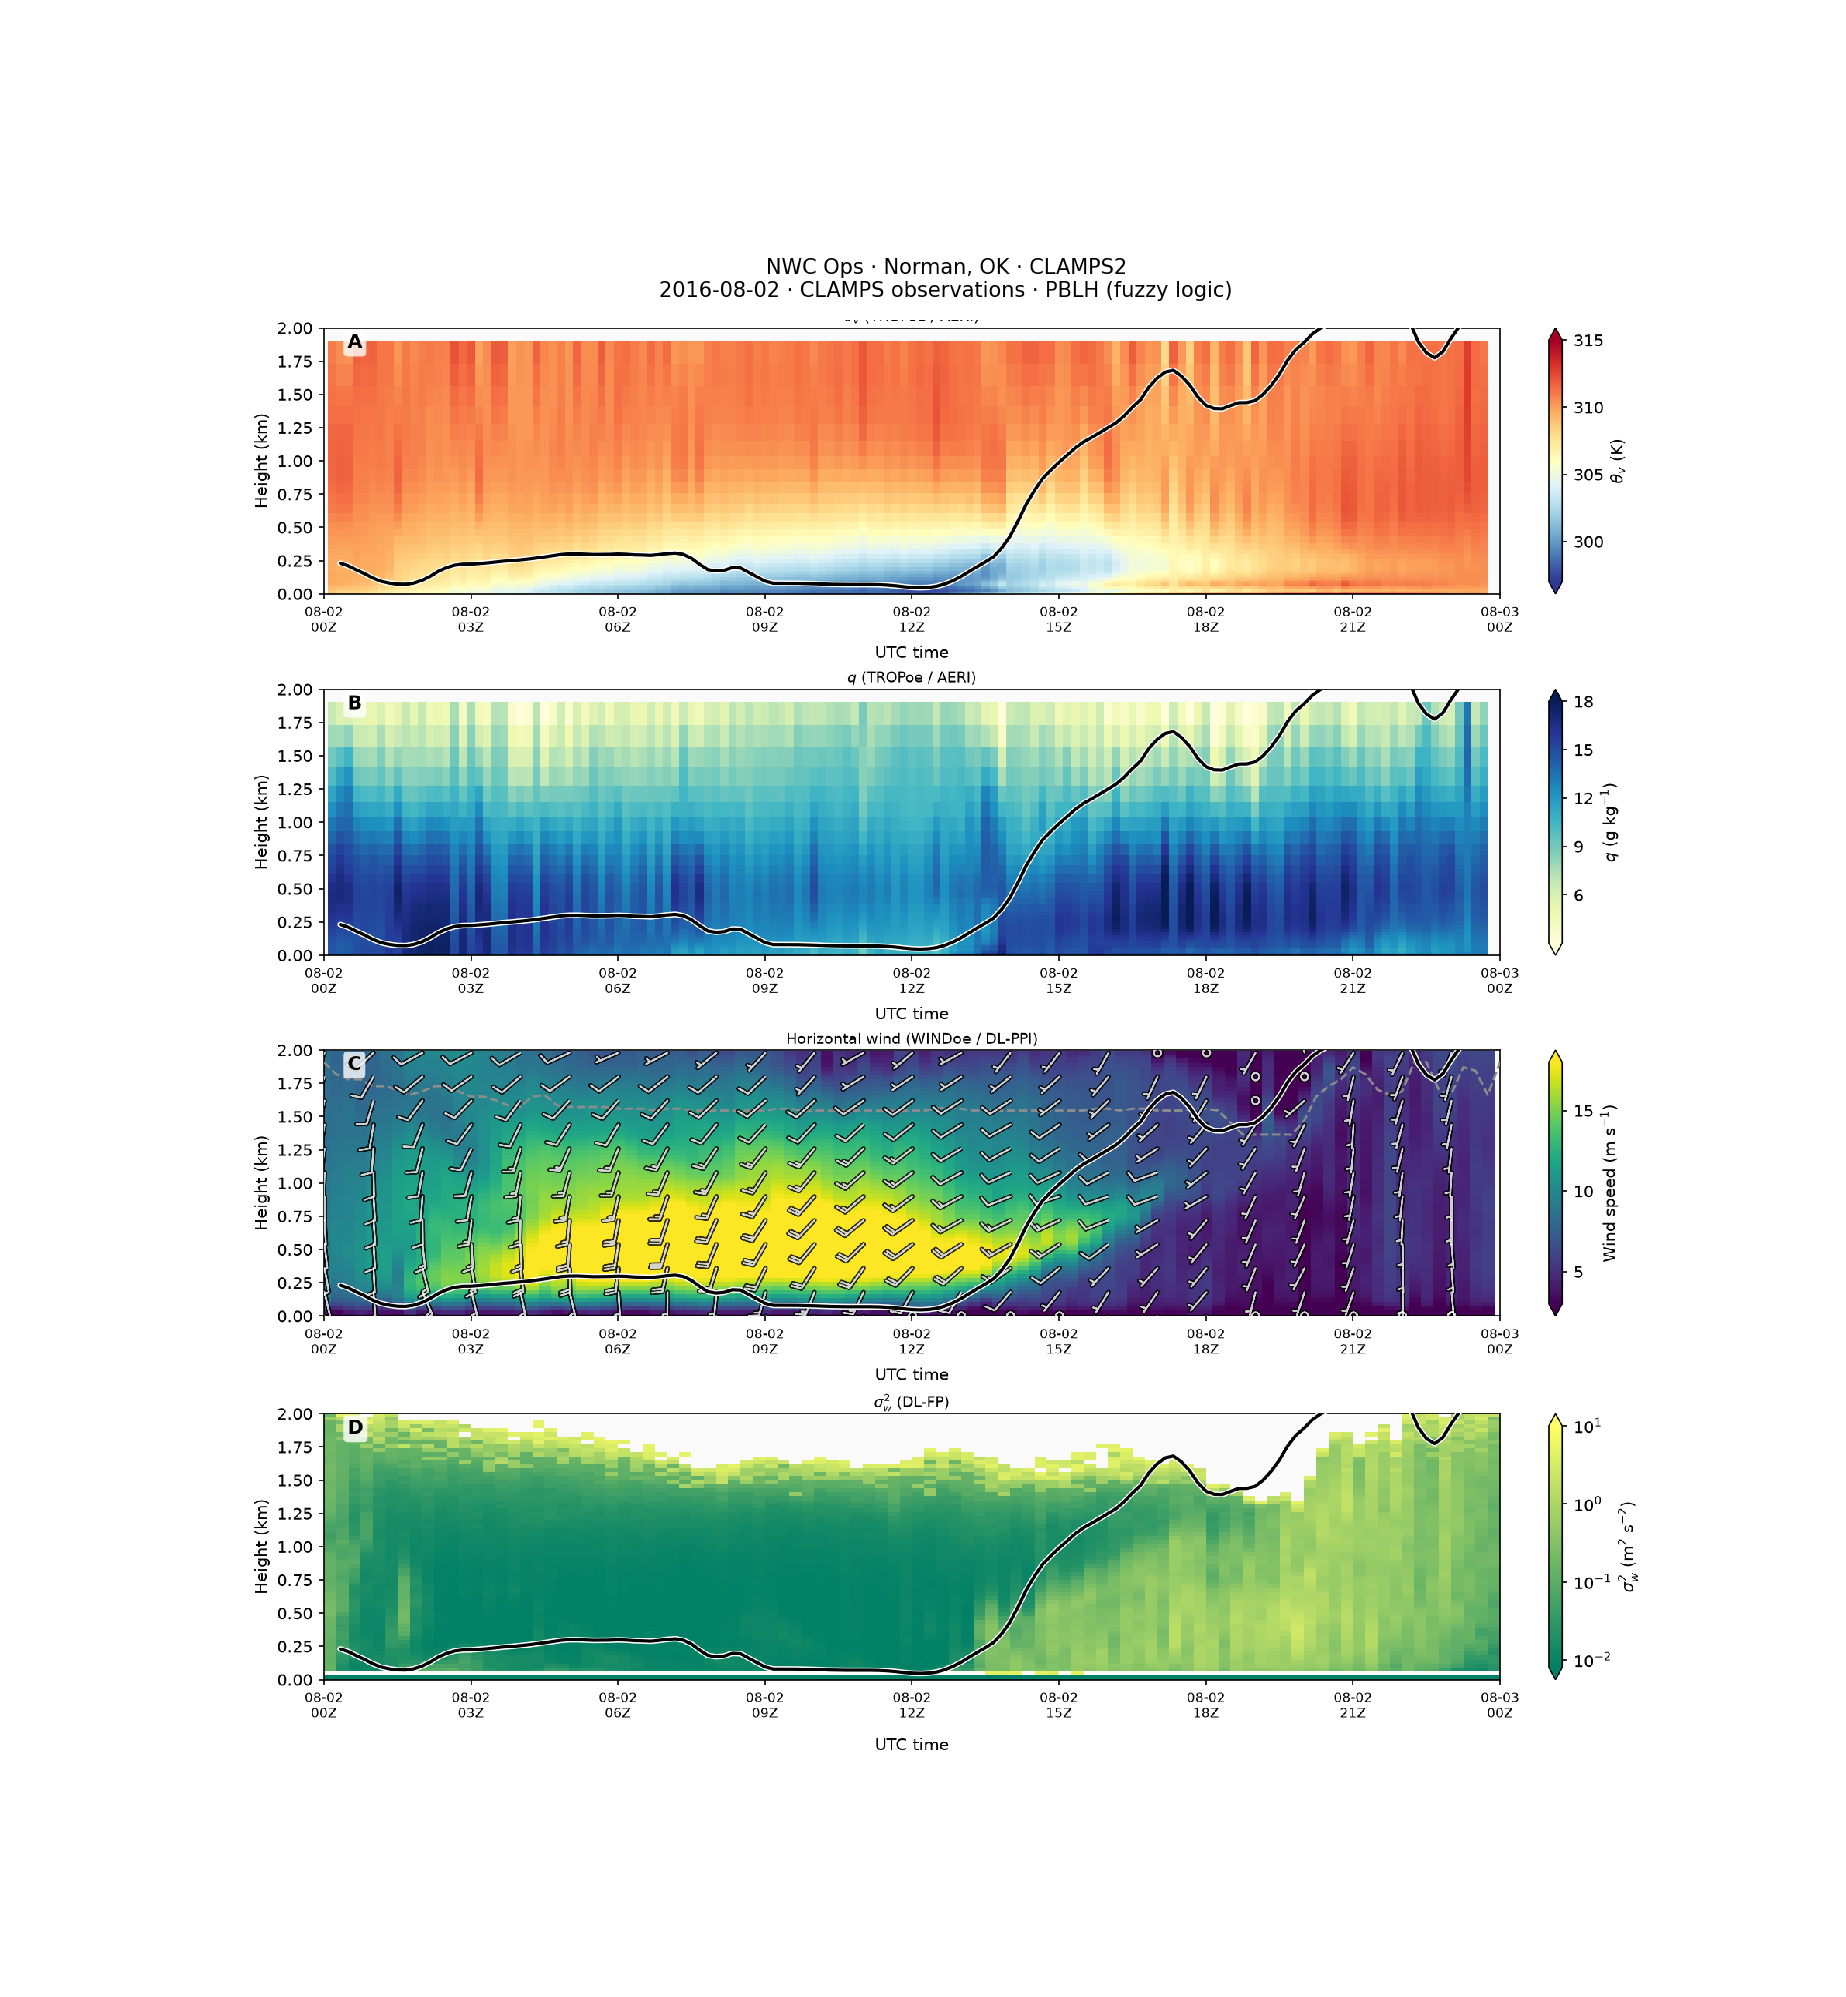
\includegraphics[width=\textwidth]{../../images/nllj_c2_instrument_template_4panel.png}
  \caption{Standard CLAMPS observations.}
  \label{fig:nllj_c2:nllj_c2_instrument_template_4panel}
\end{figure}
\subsection*{Case overview}
This case showcases a classic, strongly developed Nocturnal Low-Level Jet (NLLJ) observed by CLAMPS2 in Norman, Oklahoma. As the daytime convective mixing ceases early in the period, a sharp surface-based inversion forms, decoupling the residual layer from surface friction. This triggers a classic inertial oscillation, accelerating southerly winds within the lower kilometer of the atmosphere. Overnight, a distinct veering (clockwise turning) of the wind profile is evident both with height—shifting from southerly at the surface to south-westerly above the jet core in a response to warm air advection—and over time as the inertial wave evolves. The jet reaches its peak intensity during the overnight hours before rapidly mixing out after sunrise as the daytime convective boundary layer (CBL) develops

\subsection*{Highlights}
\begin{itemize}
  \item Thermal Structure \& Inversion (Standard CLAMPS Observations, Panel A): Following 03:00 UTC, the virtual potential temperature ($\theta_v$) shows the rapid development of a strong surface-based stable layer (indicated by the cooler blue/white shading near the surface). Convective heating begins around 12:00–13:00 UTC, driving a rapid rise in the fuzzy-logic Planetary Boundary Layer Height (PBLH) from \textasciitilde{}250 m up to 1.75 km by late afternoon. These thermodynamic variations are further detailed by the discrete profile snapshots in \hyperref[fig:nllj_c2:nllj_c2_aux_vertical_profiles_peak_jet]{Vertical profiles at peak jet}.
  \item Moisture Transport (Standard CLAMPS Observations, Panel B): Strong southerly advection maintains a deep layer of high specific humidity ($q \approx 12\text{ to } 15\text{ g kg}^{-1}$) below 1.0 km throughout the nocturnal period, providing the classic moisture-tongue setup typical of Great Plains high-impact weather environments.
  \item The Jet Core (Standard CLAMPS Observations, Panel C): The NLLJ becomes clearly defined by 03:00 UTC, with a core height centered between 250 m and 600 m. Peak horizontal wind speeds exceed $15\text{ m s}^{-1}$ between 04:00 UTC and 10:00 UTC. The wind barbs show remarkably steady southerly-to-southwesterly flow throughout the jet's lifespan. The physical mechanism of this acceleration is dynamically demonstrated at 600 m AGL by the clockwise ageostrophic wind loop in \hyperref[fig:nllj_c2:nllj_c2_aux_io_hodograph]{I/O hodograph}.
  \item Turbulence \& Mixing (Standard CLAMPS Observations, Panel D): The Doppler Lidar vertical velocity variance ($\sigma_w^2$) shows an exceptionally quiet nocturnal boundary layer beneath the jet core. However, right around 13:00 UTC, a stark explosion of turbulent kinetic energy tracks perfectly with the rising PBLH, marking the breakdown of the jet via solar heating and convective thermals. This transition is captured at high-frequency resolution in the un-averaged vertical velocity staring scan of \hyperref[fig:nllj_c2:nllj_c2_aux_raw_w_timeheight]{Raw vertical velocity time–height}.
\end{itemize}
\begin{figure}[htbp]
  \centering
  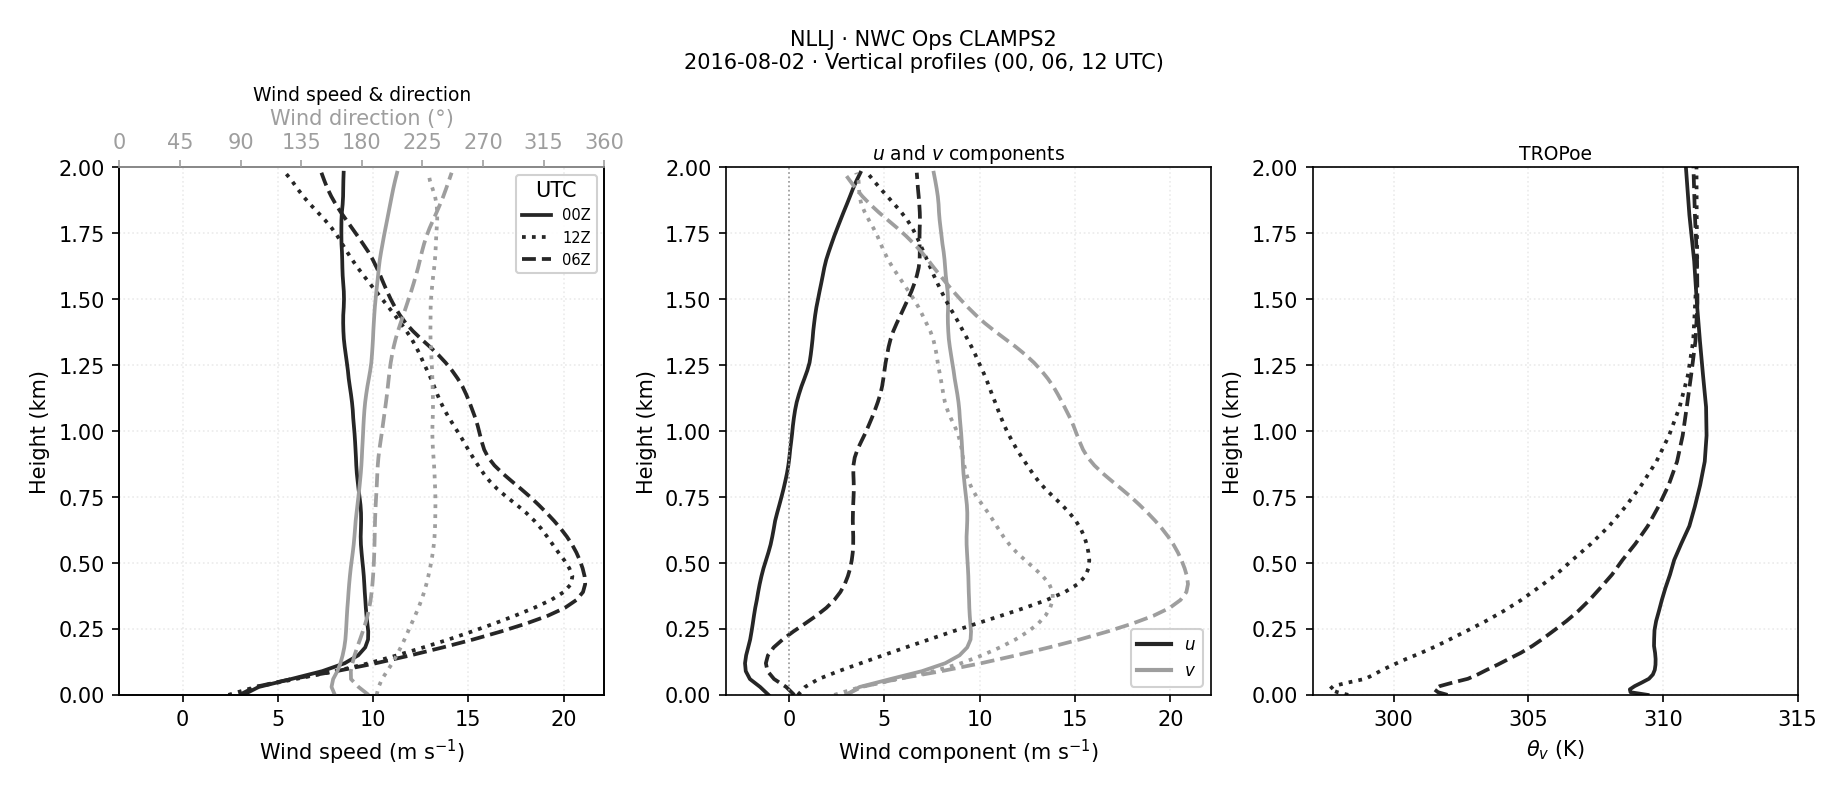
\includegraphics[width=0.92\textwidth]{../../images/nllj_c2_aux_vertical_profiles_peak_jet.png}
  \caption{Vertical profiles at peak jet.
  Line profiles of virtual potential temperature and specific humidity during peak NLLJ intensity, resolving the sharp surface inversion and jet-core thermodynamic structure.}
  \label{fig:nllj_c2:nllj_c2_aux_vertical_profiles_peak_jet}
\end{figure}
\begin{figure}[htbp]
  \centering
  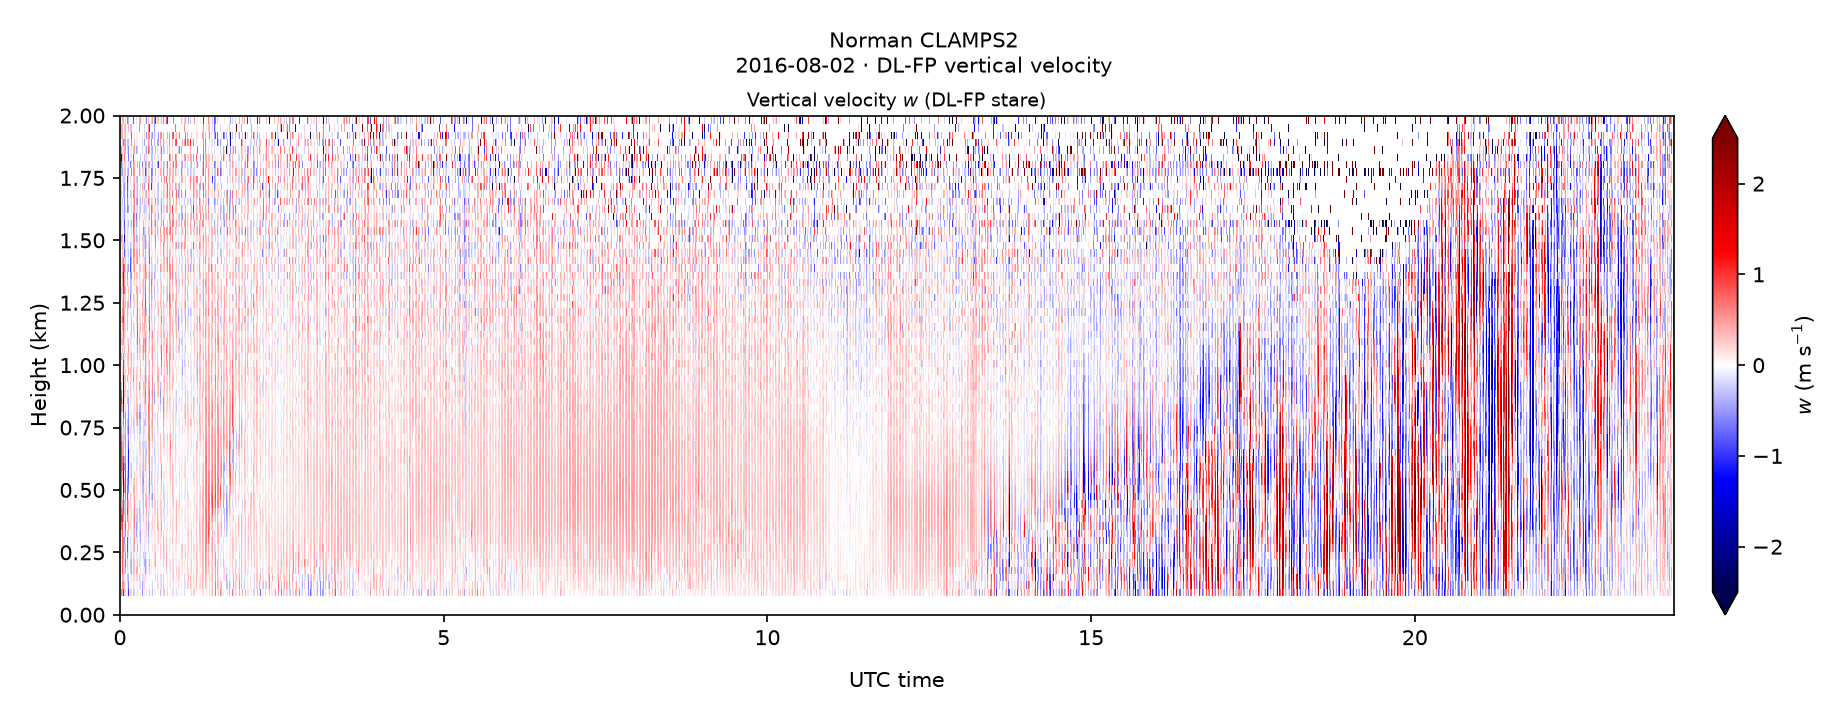
\includegraphics[width=0.92\textwidth]{../../images/nllj_c2_aux_raw_w_timeheight.png}
  \caption{Raw vertical velocity time–height.
  Unfiltered Doppler lidar vertical velocity ($w$) from zenith stares, capturing the abrupt onset of convective mixing as the nocturnal jet breaks down after sunrise.}
  \label{fig:nllj_c2:nllj_c2_aux_raw_w_timeheight}
\end{figure}
\begin{figure}[htbp]
  \centering
  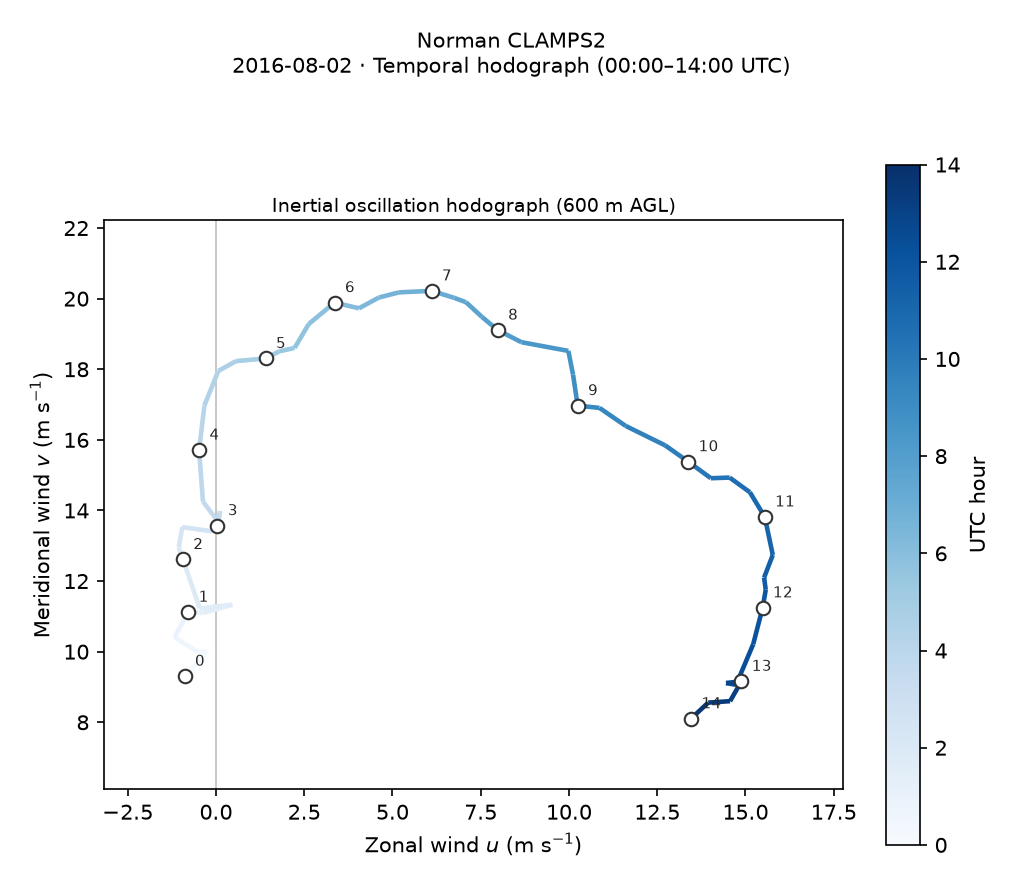
\includegraphics[width=0.92\textwidth]{../../images/nllj_c2_aux_io_hodograph.png}
  \caption{I/O hodograph.
  Inertial-oscillation hodograph at 600 m AGL showing the clockwise ageostrophic wind rotation that drives NLLJ acceleration overnight.}
  \label{fig:nllj_c2:nllj_c2_aux_io_hodograph}
\end{figure}
\section{Cold Pool}
\textit{CLAMPS2 $\cdot$ NWC Ops $\cdot$ Norman, OK $\cdot$ September 17, 2016 $\cdot$ convection, cold pool, outflow, boundaries}

\begin{figure}[htbp]
  \centering
  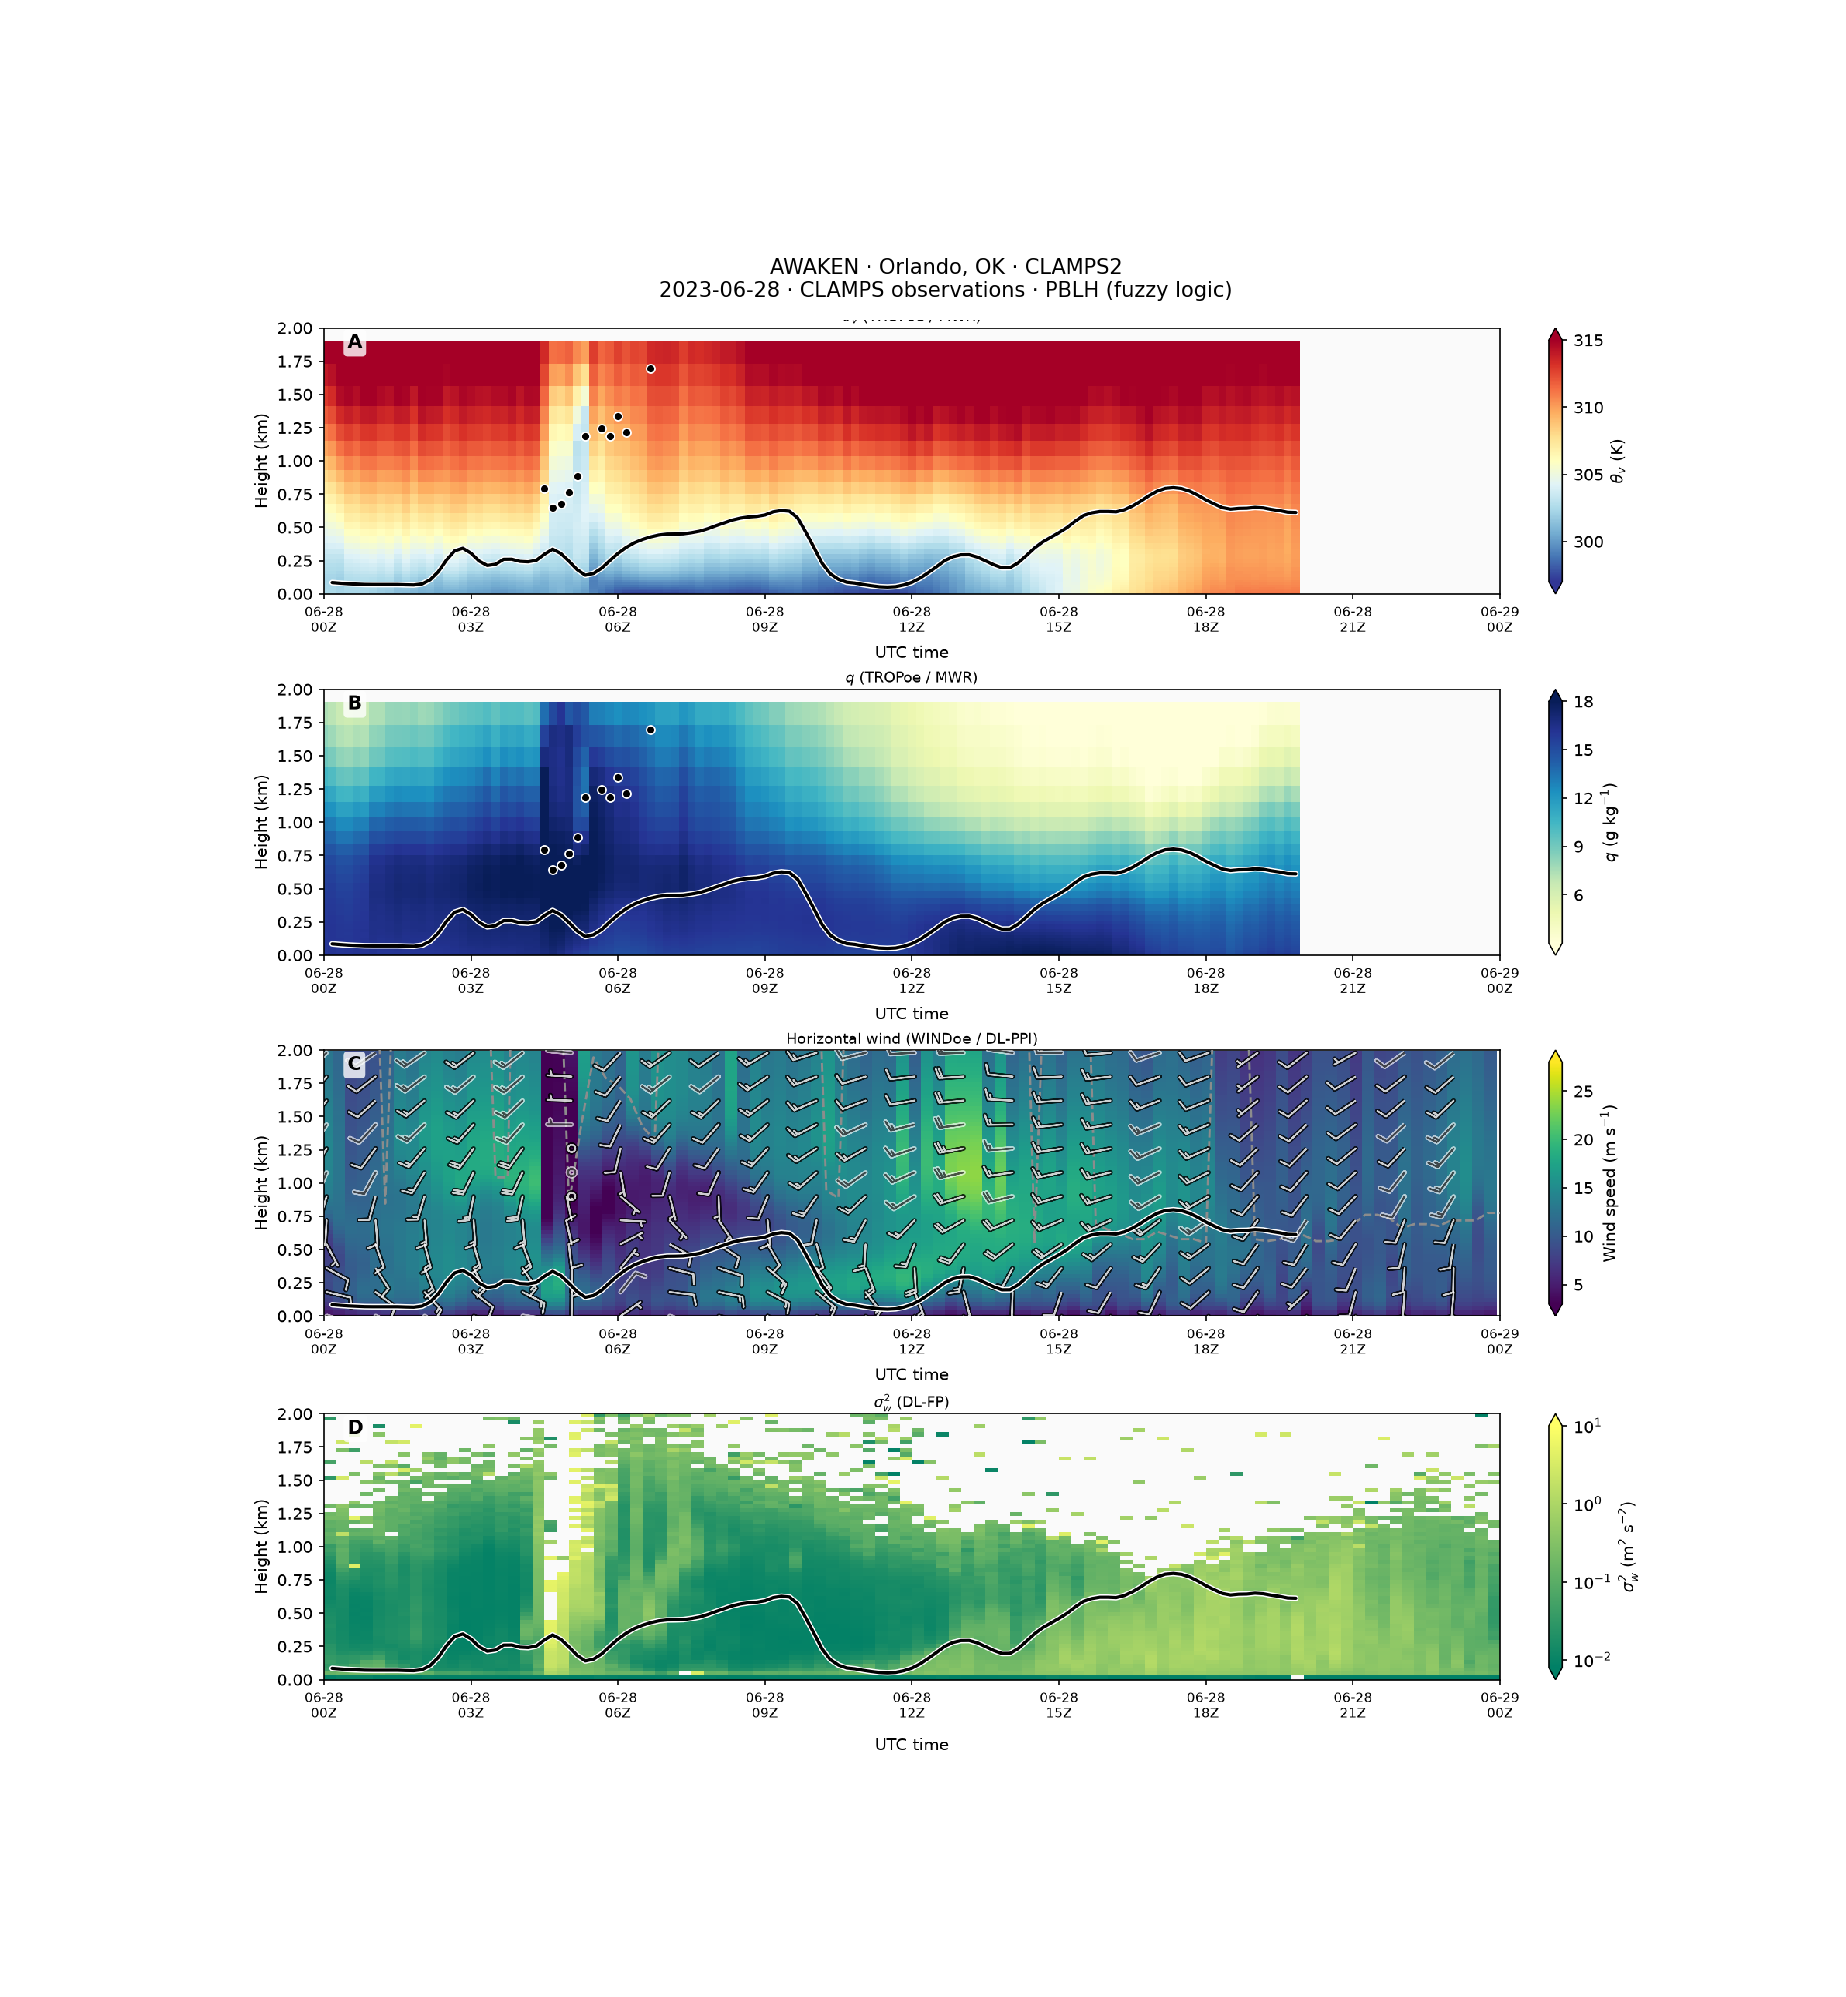
\includegraphics[width=\textwidth]{../../images/cold_pool_c2_instrument_template_4panel.png}
  \caption{Standard CLAMPS observations.}
  \label{fig:cold_pool_c2:cold_pool_c2_instrument_template_4panel}
\end{figure}
\subsection*{Case overview}
This case documents a convective cold-pool event observed by CLAMPS2 in Norman, Oklahoma during NWC Ops on 17 September 2016. The standard 4-panel view captures the full UTC day, while auxiliary figures focus on the evening transition when outflow-modified boundary-layer structure is most evident. A high-cadence (5 min) WINDoe retrieval from 18–00 UTC is used in the zoom panel to resolve wind evolution with finer temporal detail than the daily 15 min product. Surface context comes from the Norman Mesonet station (NRMN), and KTLX radar imagery provides regional convective context around 20 UTC.

\subsection*{Highlights}
\begin{itemize}
  \item Cold-pool thermodynamic signature (Panels A \& B): In \hyperref[fig:cold_pool_c2:cold_pool_c2_instrument_template_4panel]{Standard CLAMPS observations}, the virtual potential temperature ($\theta_v$) and specific humidity ($q$) fields track standard diurnal boundary layer growth up to 1.5 km before being severely modified by a convective outflow boundary at 22:00 UTC. The arrival of the cold pool violently drives temperatures down, locking in a shallow, highly stable surface layer beneath 500 m while drier environmental air remains suspended aloft.
  \item Kinematic reorganization (Panel C): The horizontal wind profile in panel C of \hyperref[fig:cold_pool_c2:cold_pool_c2_instrument_template_4panel]{Standard CLAMPS observations} captures a dramatic low-level flow adjustment as the density current arrives. This kinematic shift is captured at high-frequency resolution by the 5 min WINDoe wind speed retrieval in the lower panel of \hyperref[fig:cold_pool_c2:cold_pool_c2_aux_zoom_w_wspd_18_00utc]{Evening zoom: $w$ and wind speed (18–00 UTC)}, which details an instantaneous acceleration from a calm pre-frontal state ($< 4\text{ m s}^{-1}$) to an intense low-level surge exceeding $10\text{ m s}^{-1}$ behind the head.
  \item DL-FP vertical motion (Panel D and zoom): The Doppler Lidar vertical velocity variance ($\sigma_w^2$, panel D of \hyperref[fig:cold_pool_c2:cold_pool_c2_instrument_template_4panel]{Standard CLAMPS observations}) transitions from buoyant afternoon thermals to an intense burst of shear-generated turbulence at 22:00 UTC. The full-day stare mode in \hyperref[fig:cold_pool_c2:cold_pool_c2_aux_dlfp_w_timeheight]{DL-FP vertical velocity time–height} reveals that this boundary-layer collapse is triggered by a classic narrow, high-velocity updraft-downdraft couplet at the cold-pool head.
  \item Evening fine-scale structure (18–00 UTC zoom): The two-panel zoom in \hyperref[fig:cold_pool_c2:cold_pool_c2_aux_zoom_w_wspd_18_00utc]{Evening zoom: $w$ and wind speed (18–00 UTC)} couples high-resolution DL-FP $w$ with 5 min WINDoe wind profiles. This layout isolates the short-period gravity wave features and deep, localized downward subsidence (dark blue core hitting $-2\text{ m s}^{-1}$) as the density current sweeps across the platform.
  \item Surface verification (Mesonet): The independent surface constraints in \hyperref[fig:cold_pool_c2:cold_pool_c2_aux_surface_meteogram]{OK Mesonet surface meteogram (NRMN)} confirm the microphysical timing of the cold pool's arrival at 22:00 UTC. The meteogram logs a violent $10^\circ\text{C}$ temperature crash, a sharp $3\text{ hPa}$ hydrostatic pressure jump, an immediate wind shift from southeasterly to a northerly gust front peaking near $15\text{ m s}^{-1}$, and a heavy rainfall rate exceeding $20\text{ mm h}^{-1}$.
  \item Regional context (KTLX): The base reflectivity and radial velocity loops in \hyperref[fig:cold_pool_c2:cold_pool_c2_ktlx_20160917_2000]{KTLX radar reflectivity (20 UTC)} provide the synoptic catalyst for this event. At 20:07 UTC, radar imagery captures a severe convective cell with a high-reflectivity core centered just west of Norman near Minco and Tuttle, pushing a distinct, outrunning radial velocity discontinuity line (gust front) eastward directly toward the CLAMPS2 testing pad.
\end{itemize}
\begin{figure}[htbp]
  \centering
  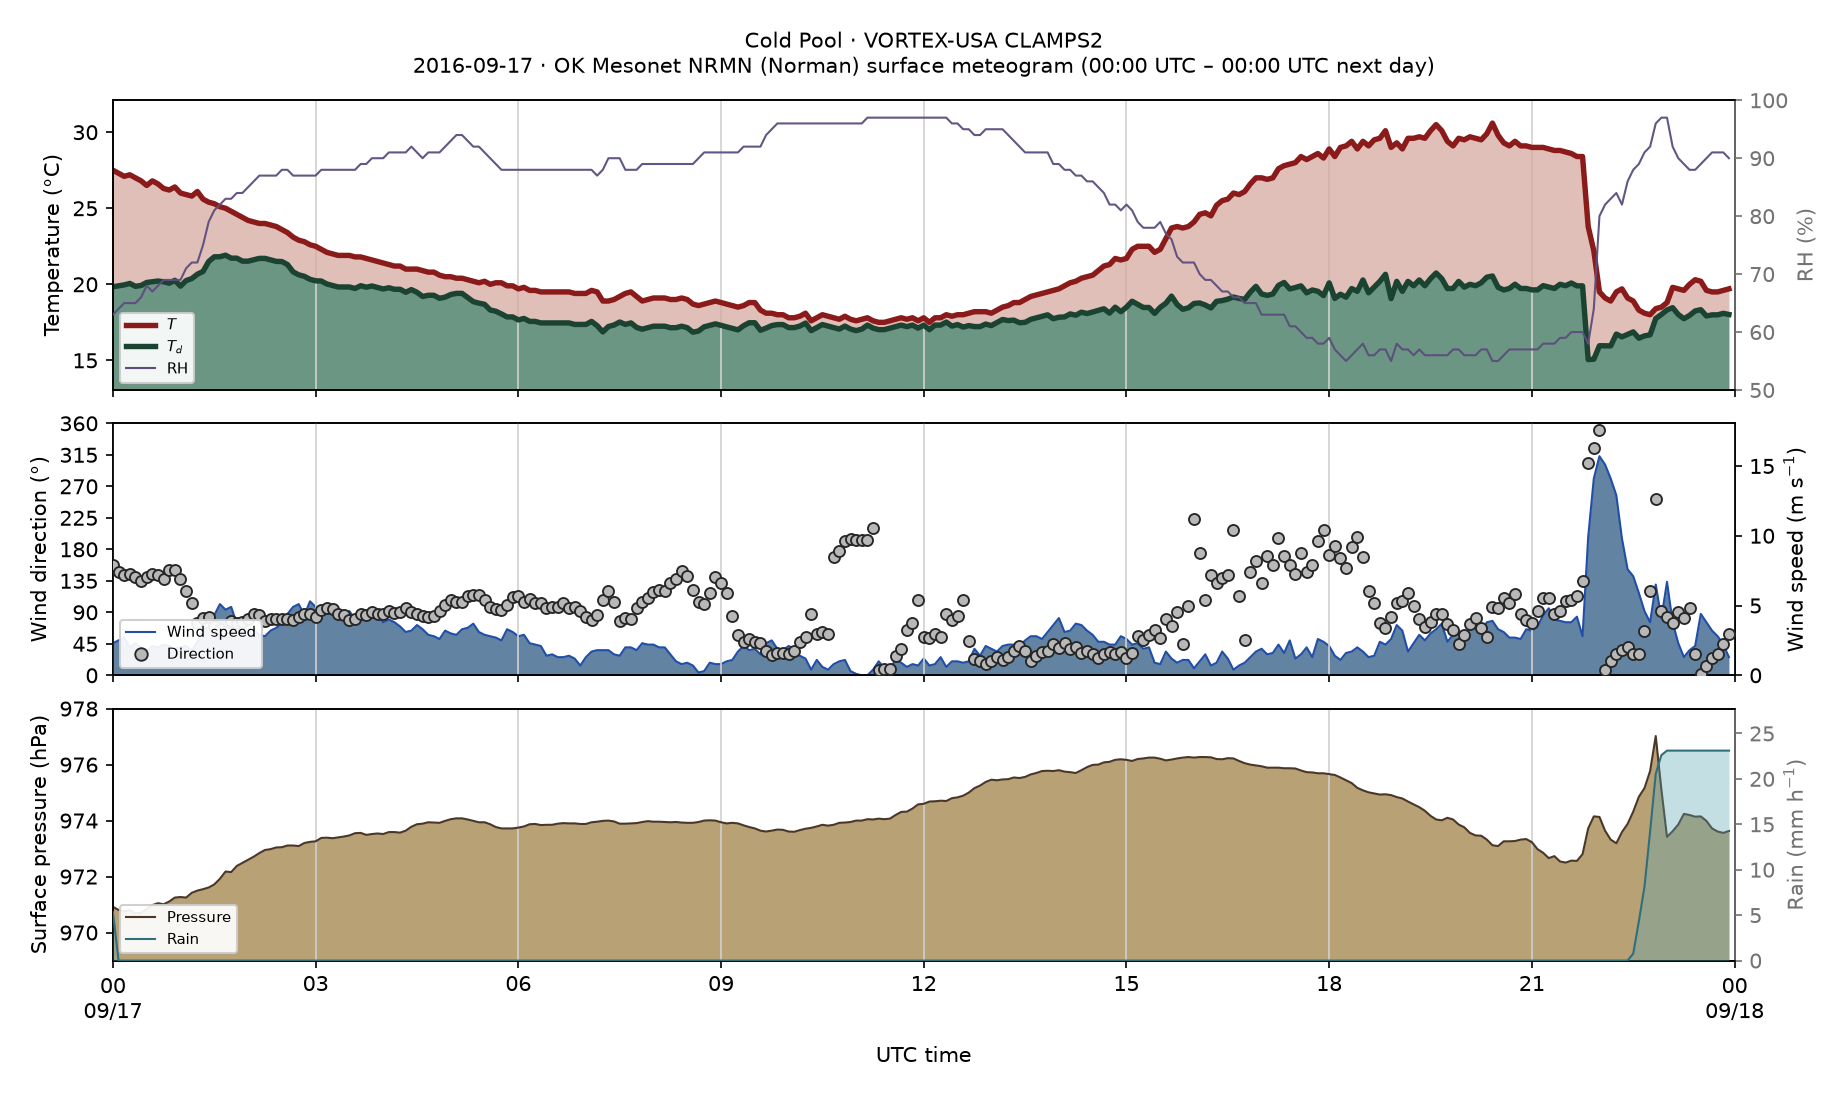
\includegraphics[width=0.92\textwidth]{../../images/cold_pool_c2_aux_surface_meteogram.png}
  \caption{OK Mesonet surface meteogram (NRMN).
  Oklahoma Mesonet NRMN meteogram verifying the 22:00 UTC cold-pool arrival with $10^\circ\mathrm{C}$ temperature crash, $3$ hPa pressure jump, northerly gust front, and heavy rainfall.}
  \label{fig:cold_pool_c2:cold_pool_c2_aux_surface_meteogram}
\end{figure}
\begin{figure}[htbp]
  \centering
  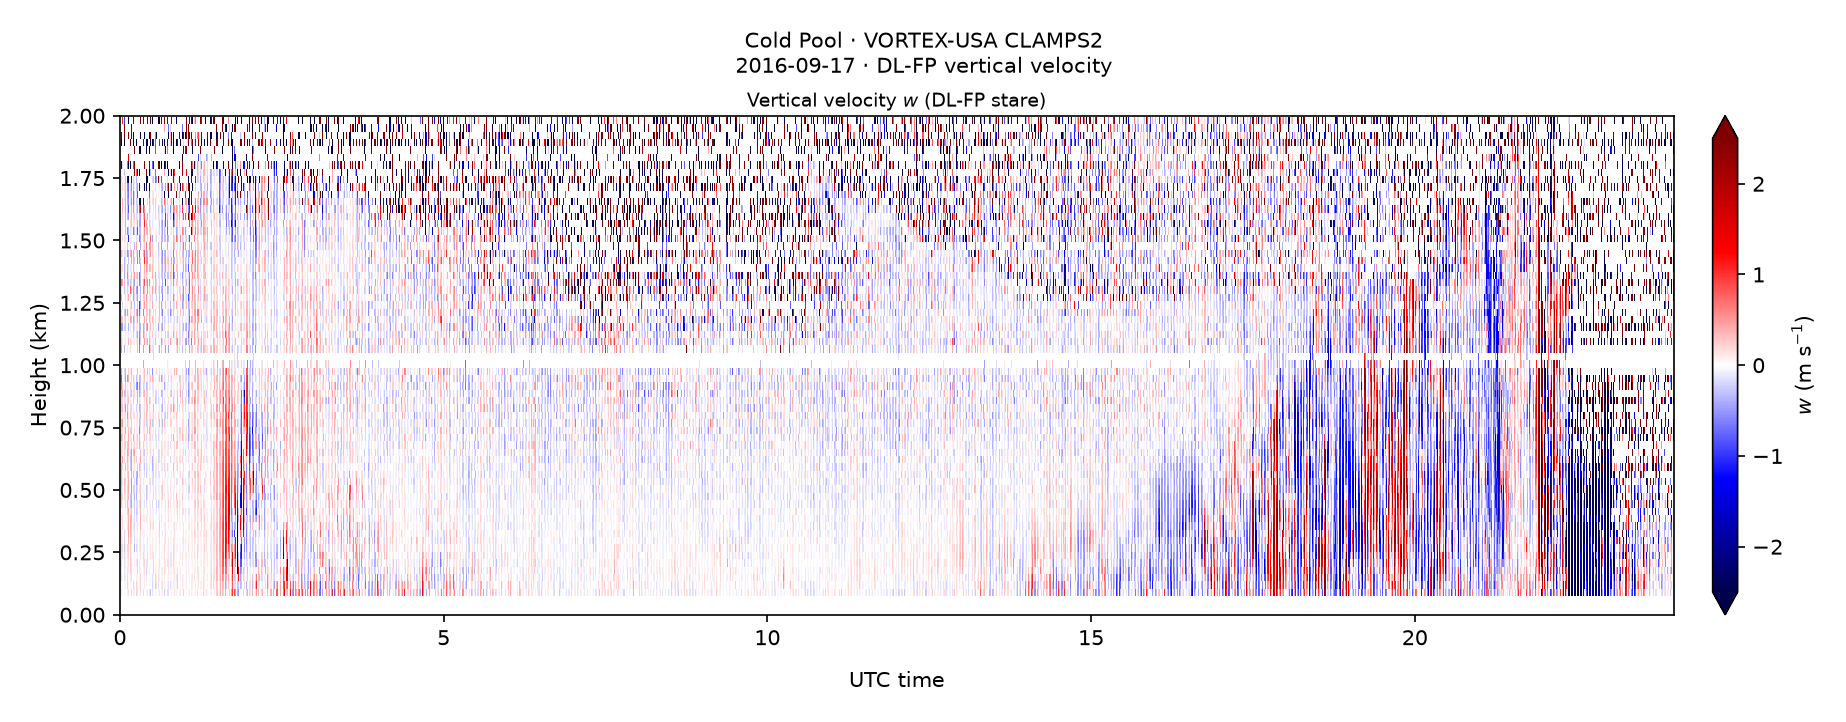
\includegraphics[width=0.92\textwidth]{../../images/cold_pool_c2_aux_dlfp_w_timeheight.png}
  \caption{DL-FP vertical velocity time–height.
  Full-day DL-FP vertical velocity stare resolving the narrow updraft–downdraft couplet at the cold-pool head and subsequent gravity-wave features.}
  \label{fig:cold_pool_c2:cold_pool_c2_aux_dlfp_w_timeheight}
\end{figure}
\begin{figure}[htbp]
  \centering
  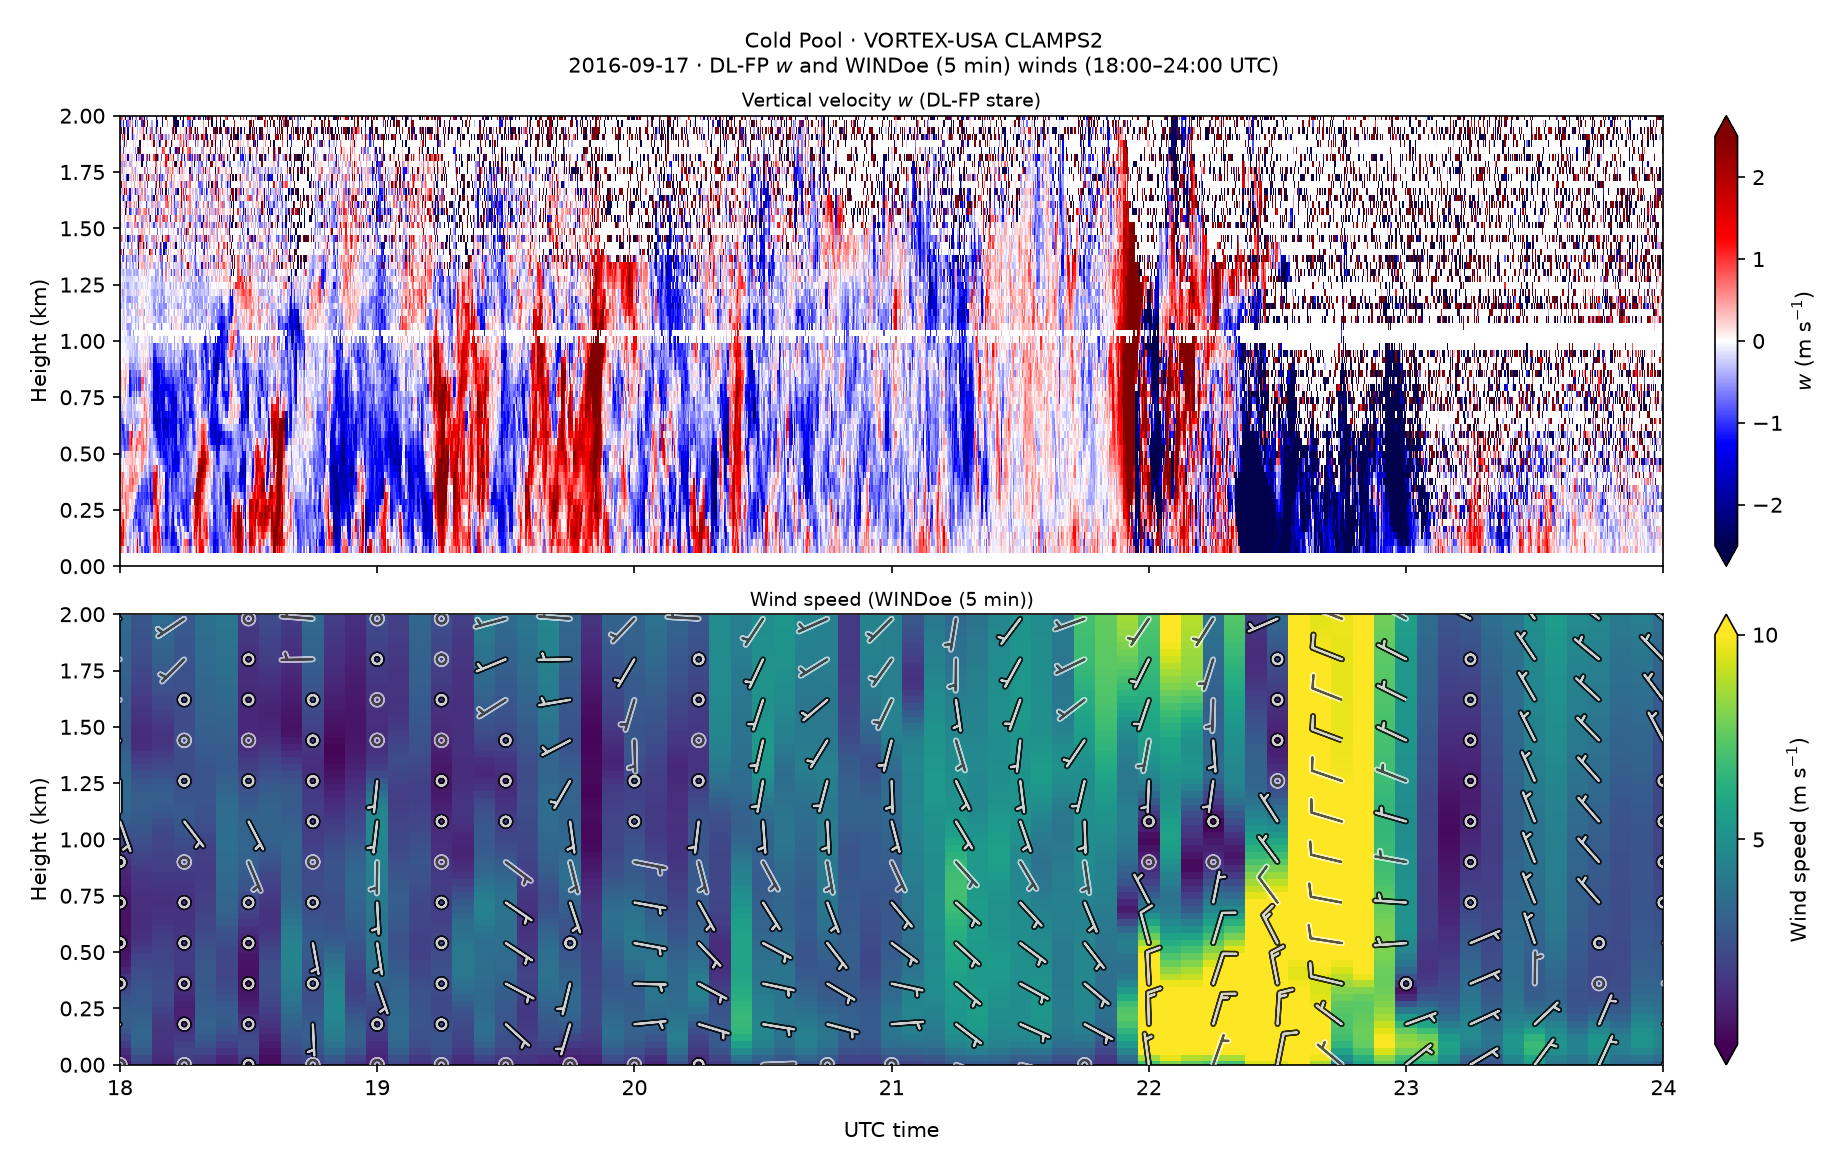
\includegraphics[width=0.92\textwidth]{../../images/cold_pool_c2_aux_zoom_w_wspd_18_00utc.png}
  \caption{Evening zoom: $w$ and wind speed (18–00 UTC).
  Evening zoom coupling high-resolution DL-FP $w$ (top) with 5 min WINDoe wind speed (bottom) during outflow passage; subsidence cores reach $-2\,\mathrm{m\,s^{-1}}$.}
  \label{fig:cold_pool_c2:cold_pool_c2_aux_zoom_w_wspd_18_00utc}
\end{figure}
\begin{figure}[htbp]
  \centering
  \includegraphics[width=0.92\textwidth]{_frames/cold_pool_c2_ktlx_20160917_2000.png}
  \caption{KTLX radar reflectivity (20 UTC).
  KTLX base reflectivity and radial velocity at 20 UTC showing the severe cell west of Norman and the outrunning gust-front discontinuity approaching the platform. First frame of animated loop; full animation available in the online gallery.}
  \label{fig:cold_pool_c2:cold_pool_c2_ktlx_20160917_2000}
\end{figure}
\section{Nocturnal Low-Level Jet}
\textit{CLAMPS1 $\cdot$ NWC Ops $\cdot$ Norman, OK $\cdot$ August 26, 2018 $\cdot$ boundary layer, nocturnal, wind}

\begin{figure}[htbp]
  \centering
  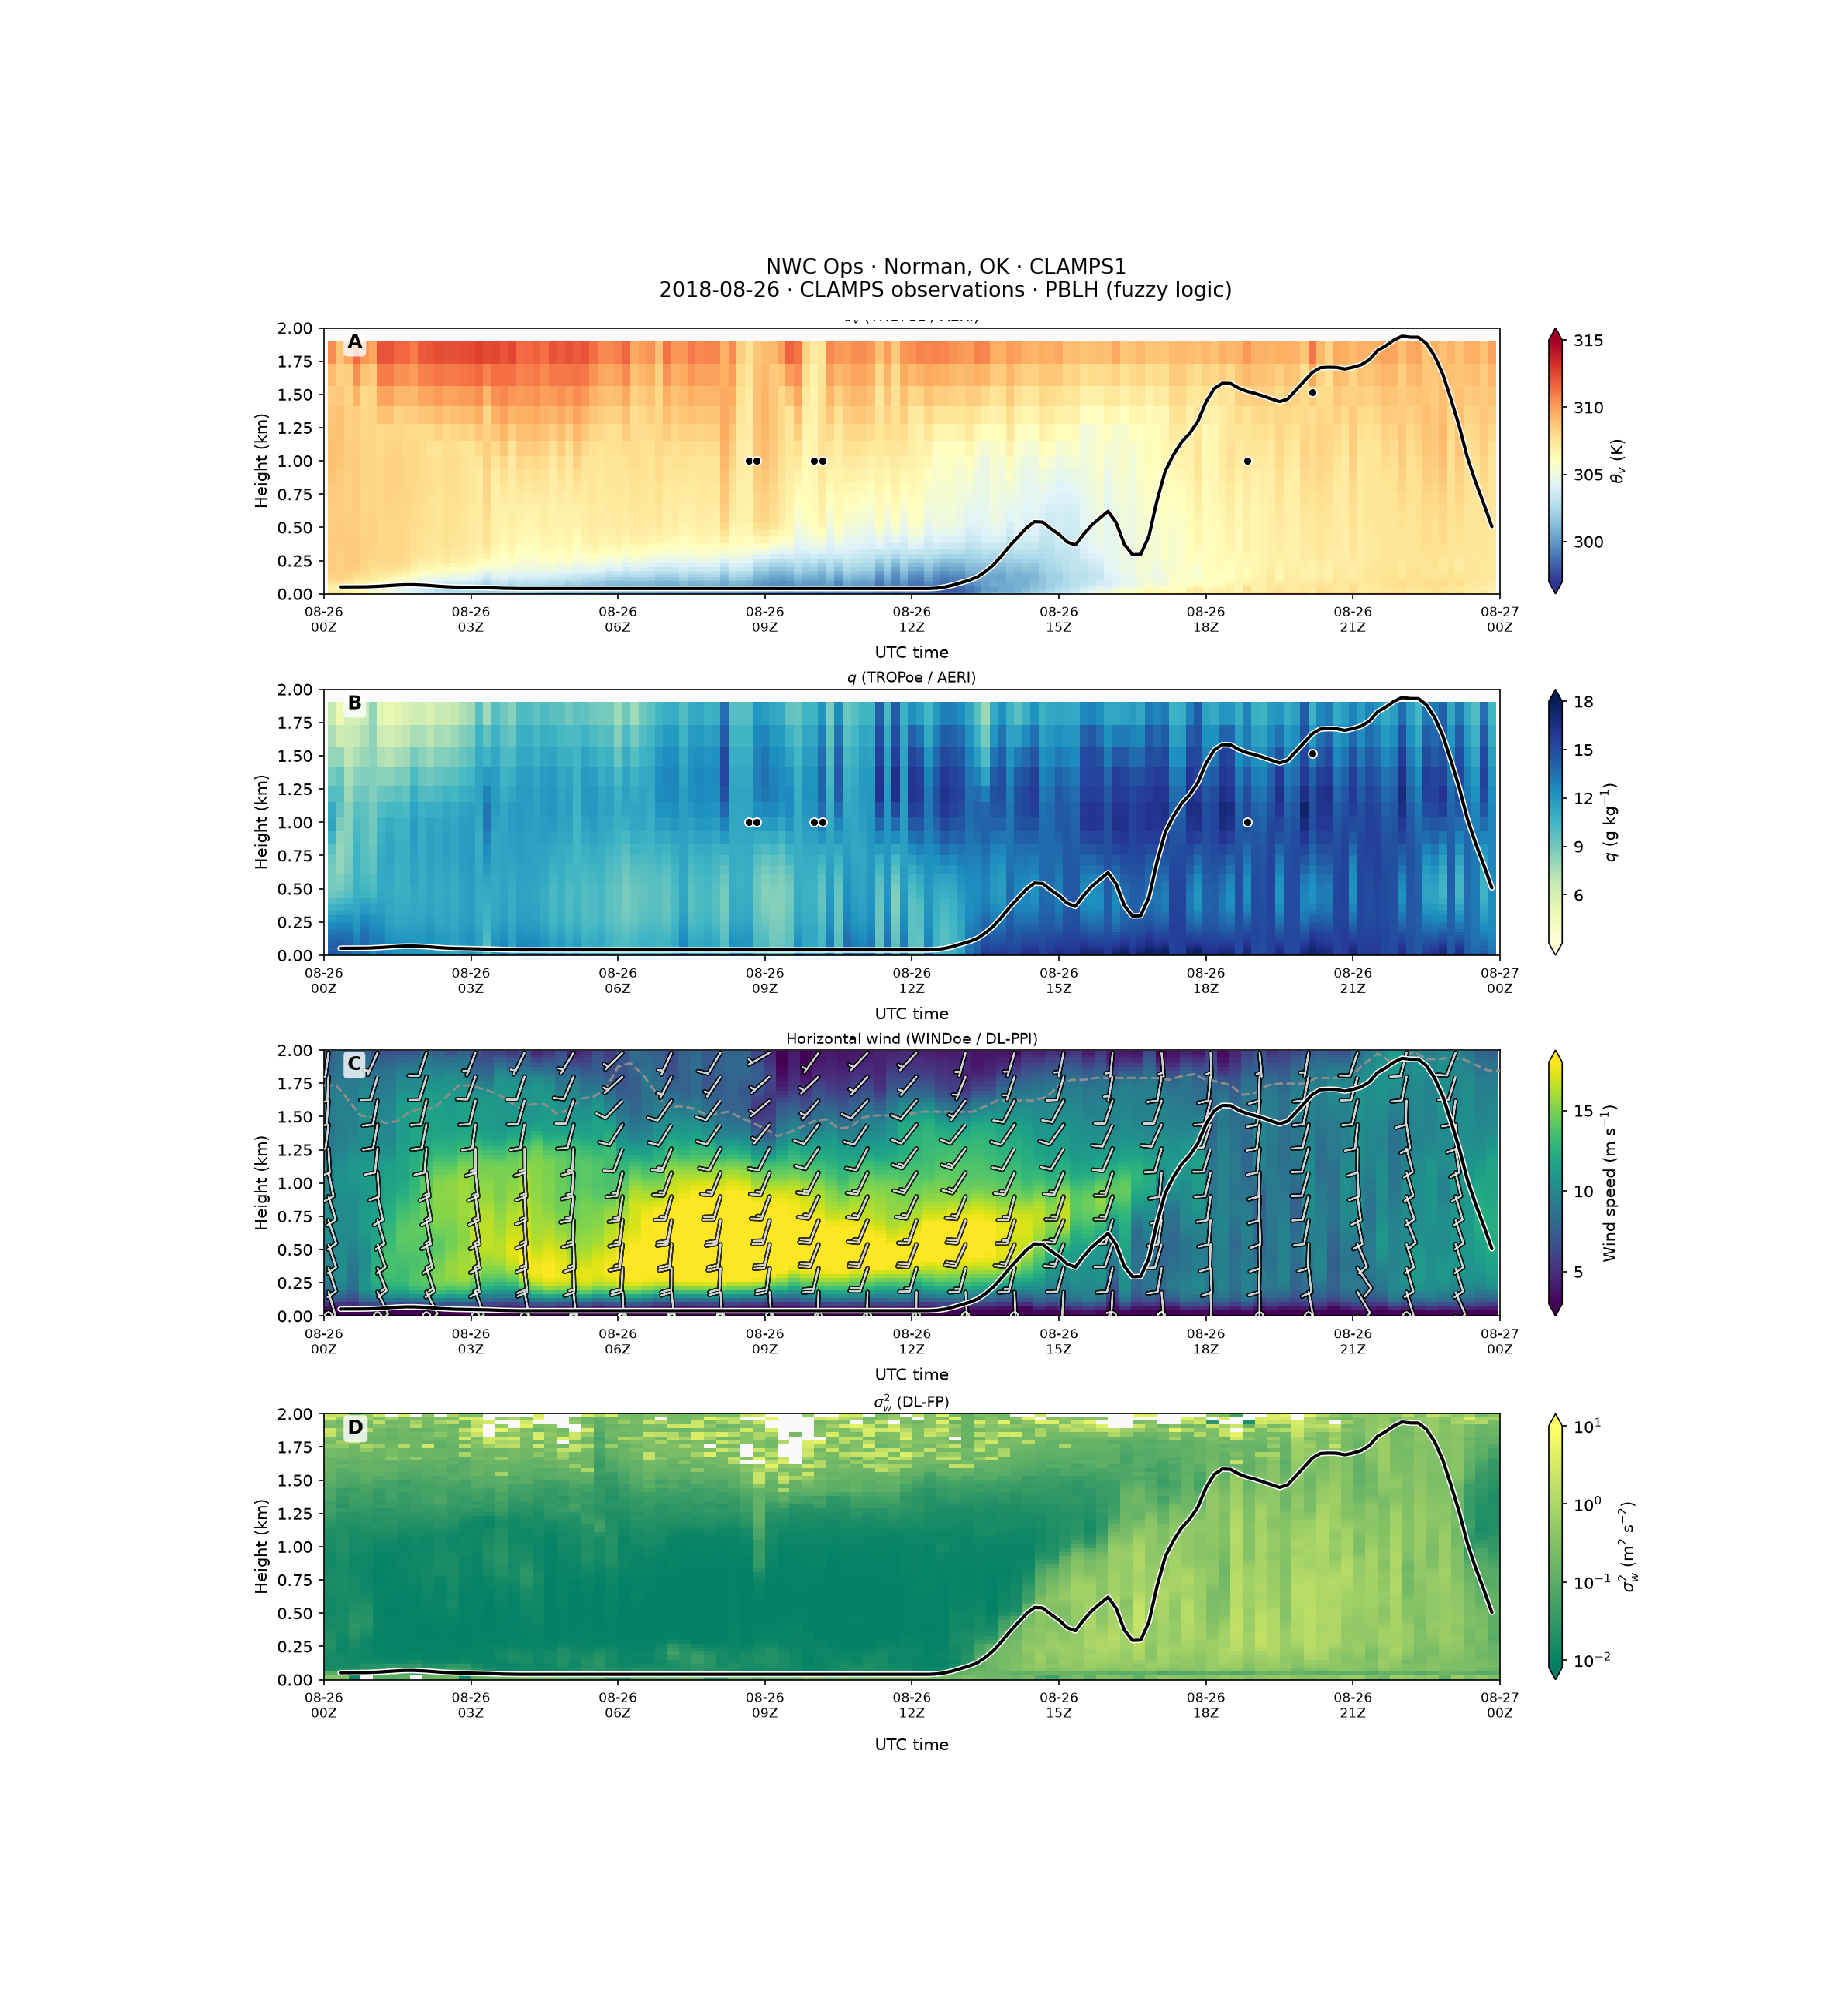
\includegraphics[width=\textwidth]{../../images/nllj_c1_instrument_template_4panel.png}
  \caption{Standard CLAMPS observations.}
  \label{fig:nllj_c1:nllj_c1_instrument_template_4panel}
\end{figure}
\subsection*{Case overview}
This case showcases a beautifully resolved, high-intensity Nocturnal Low-Level Jet (NLLJ) captured by the CLAMPS1 platform in Norman, Oklahoma. Following sunset, a rapid decoupling of the boundary layer isolates the residual layer from surface friction, instigating a classic inertial oscillation. This drives a significant acceleration of the southerly wind field just above a shallow, surface-based radiation inversion. Throughout the evening, strong veering (clockwise turning) of the wind profile is highly visible both with height and across time as the ageostrophic wind vector rotates. The jet maintains its integrity until approximately 12:00 UTC, after which solar heating triggers a rapid morning transition into a deep daytime convective boundary layer (CBL).

\subsection*{Highlights}
\begin{itemize}
  \item Thermal Structure \& Inversion (Panel A): A shallow, strong surface-based stable layer forms rapidly after 02:00 UTC, keeping the immediate surface cool ($\theta_v < 300\text{ K}$, shown in blue/white). The morning transition begins after 12:00 UTC, showing an interesting two-stage boundary layer growth: an initial shallow convective lift to \textasciitilde{}500 m between 14:00 and 16:00 UTC, followed by a rapid burst up to nearly 1.9 km by 22:00 UTC. The progressive erosion of this thermal structure is quantitatively tracked by the multi-hour line profiles in \hyperref[fig:nllj_c1:nllj_c1_aux_vertical_profiles_peak_jet]{Vertical profiles at peak jet}.
  \item Moisture Transport (Panel B): Steady low-level advection maintains a deep layer of high specific humidity ($q \approx 11\text{ to }14\text{ g kg}^{-1}$) capped entirely below 1.0 km during the nocturnal period. Once the CBL deepens past 16:00 UTC, this moisture is efficiently mixed through the full 2.0 km column, resulting in a drop in near-surface specific humidity.
  \item The Jet Core (Panel C): The NLLJ stabilizes by 04:00 UTC, with its core centered slightly higher than the 2016 case, sitting between 500 m and 750 m. Peak horizontal wind speeds exceed $15\text{ m s}^{-1}$ (bright yellow) continuously between 05:00 and 10:00 UTC. The wind barbs capture a classic inertial rotation: at 500 m, winds clock from south-southeast at 02:00 UTC, to purely southerly at 05:00 UTC, to south-southwesterly by 09:00 UTC. This ageostrophic wind vector rotation is modeled dynamically at 600 m AGL in \hyperref[fig:nllj_c1:nllj_c1_aux_io_hodograph]{I/O hodograph}.
  \item Turbulence \& Mixing (Panel D): The Doppler Lidar vertical velocity variance ($\sigma_w^2$) highlights an extraordinarily quiescent nocturnal environment beneath the jet, with variance plunging to near-baseline levels ($10^{-2}\text{ m}^2\text{ s}^{-2}$). The daytime turbulent decay of the jet is spectacular, with thermal updrafts and downdrafts completely dominating the column after 16:00 UTC, as visually resolved in the raw time-height scan of \hyperref[fig:nllj_c1:nllj_c1_aux_raw_w_timeheight]{Raw vertical velocity time–height}.
\end{itemize}
\begin{figure}[htbp]
  \centering
  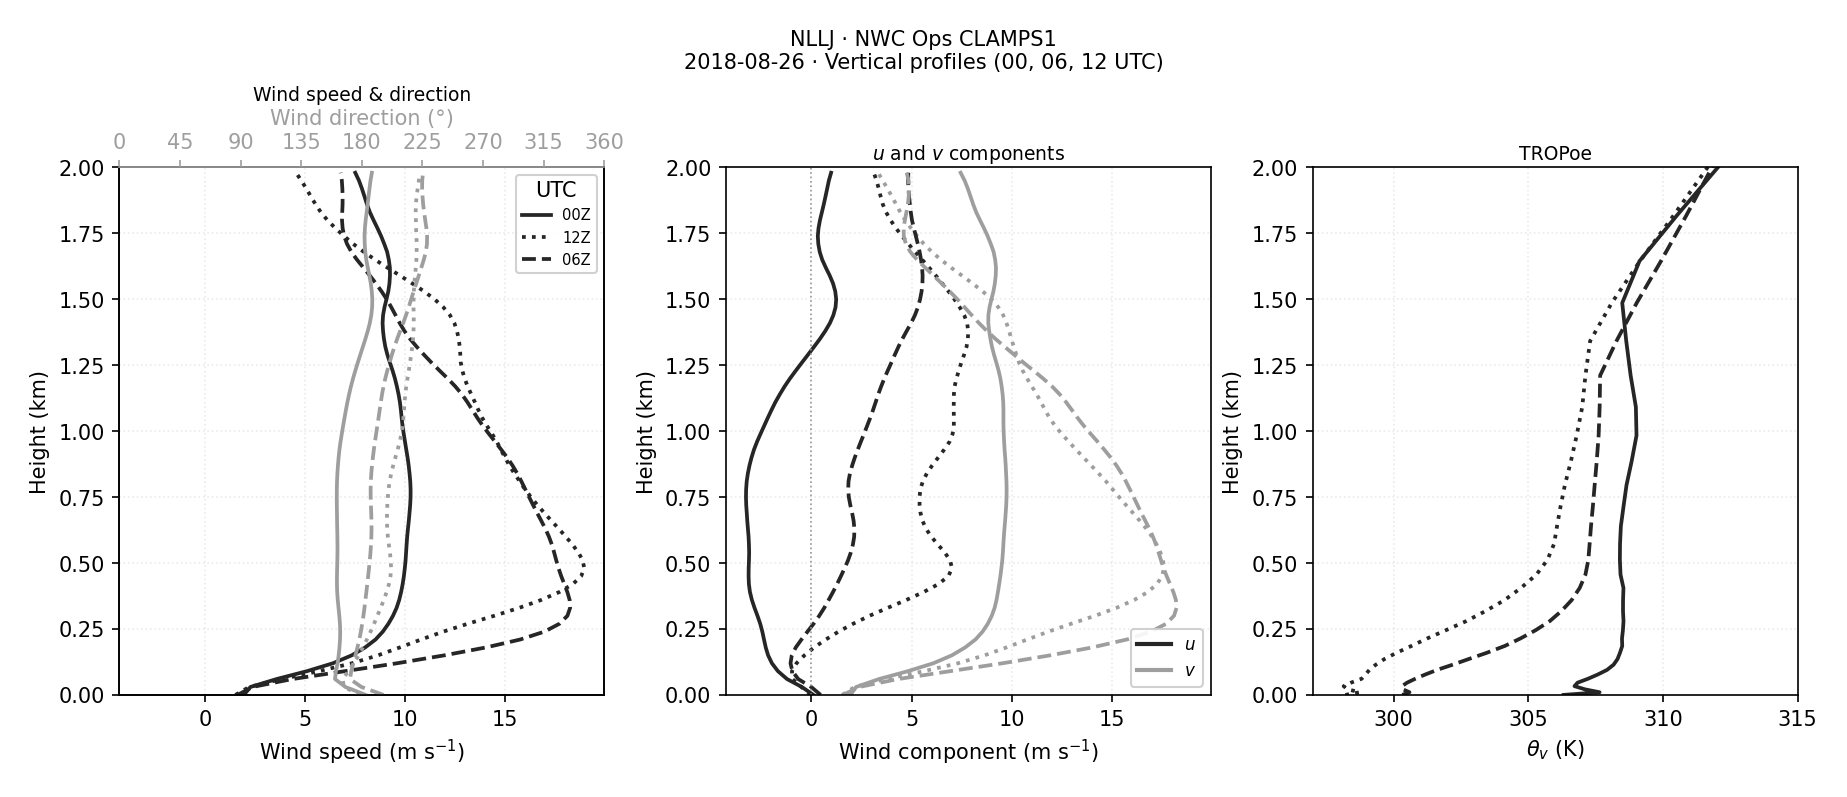
\includegraphics[width=0.92\textwidth]{../../images/nllj_c1_aux_vertical_profiles_peak_jet.png}
  \caption{Vertical profiles at peak jet.
  Multi-hour line profiles of $\theta_v$ and $q$ tracking the progressive erosion of the nocturnal inversion and two-stage morning boundary-layer growth.}
  \label{fig:nllj_c1:nllj_c1_aux_vertical_profiles_peak_jet}
\end{figure}
\begin{figure}[htbp]
  \centering
  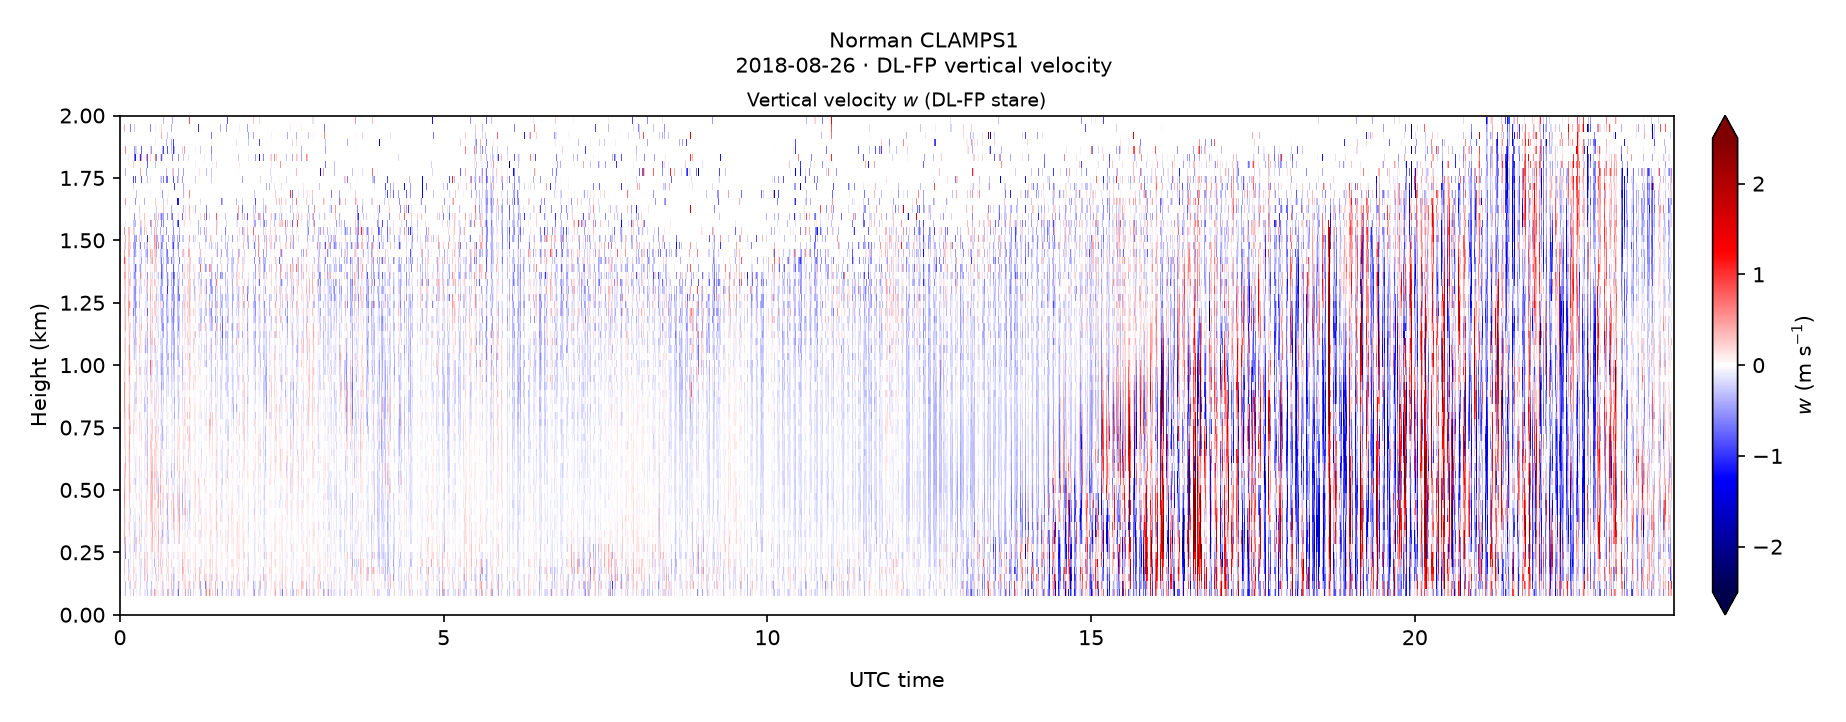
\includegraphics[width=0.92\textwidth]{../../images/nllj_c1_aux_raw_w_timeheight.png}
  \caption{Raw vertical velocity time–height.
  Raw DL-FP vertical velocity time–height scan resolving high-frequency turbulent structure during jet decay and deep convective mixing after 16:00 UTC.}
  \label{fig:nllj_c1:nllj_c1_aux_raw_w_timeheight}
\end{figure}
\begin{figure}[htbp]
  \centering
  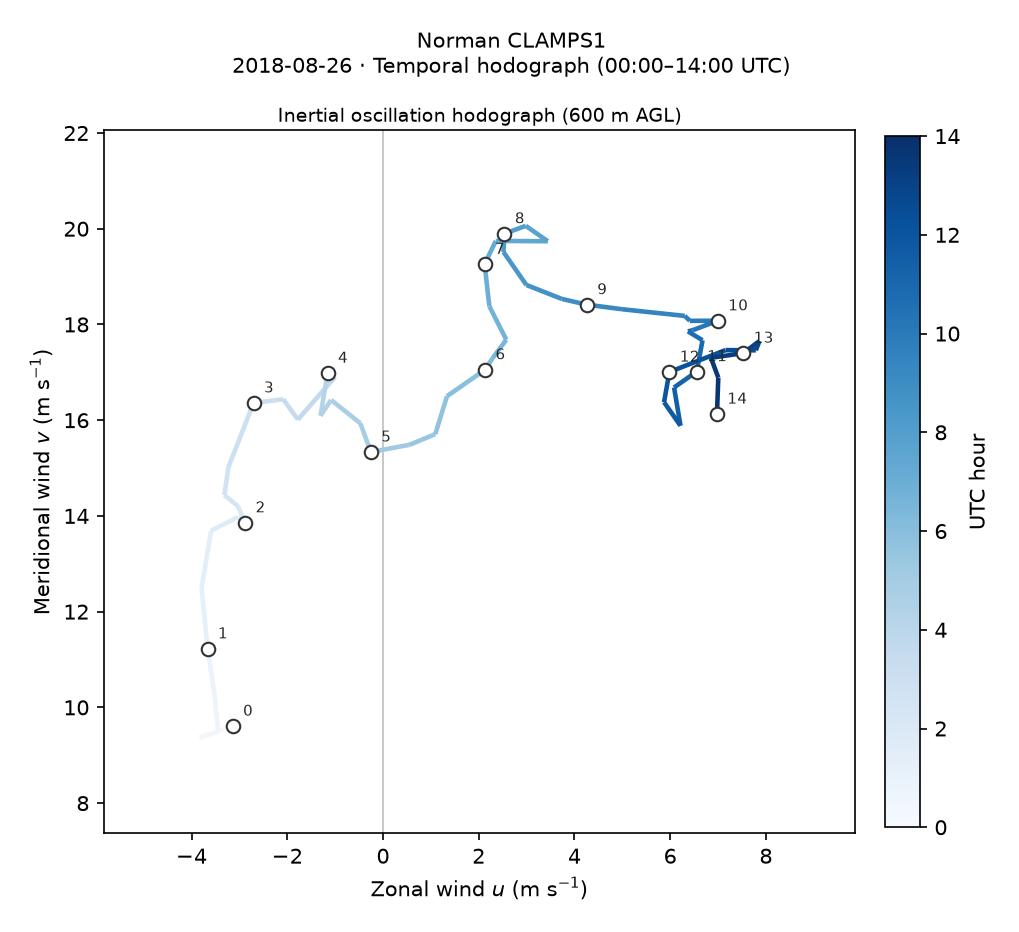
\includegraphics[width=0.92\textwidth]{../../images/nllj_c1_aux_io_hodograph.png}
  \caption{I/O hodograph.
  Hodograph at 600 m AGL modeling the inertial wind rotation from south-southeast through southerly to south-southwesterly flow within the jet core.}
  \label{fig:nllj_c1:nllj_c1_aux_io_hodograph}
\end{figure}
\section{Stable Boundary Layer — Degraded Lidar Quality}
\textit{CLAMPS1 $\cdot$ VORTEX-USA $\cdot$ Courtland, AL $\cdot$ January 25, 2019 $\cdot$ stable, limitations, winter}

\begin{figure}[htbp]
  \centering
  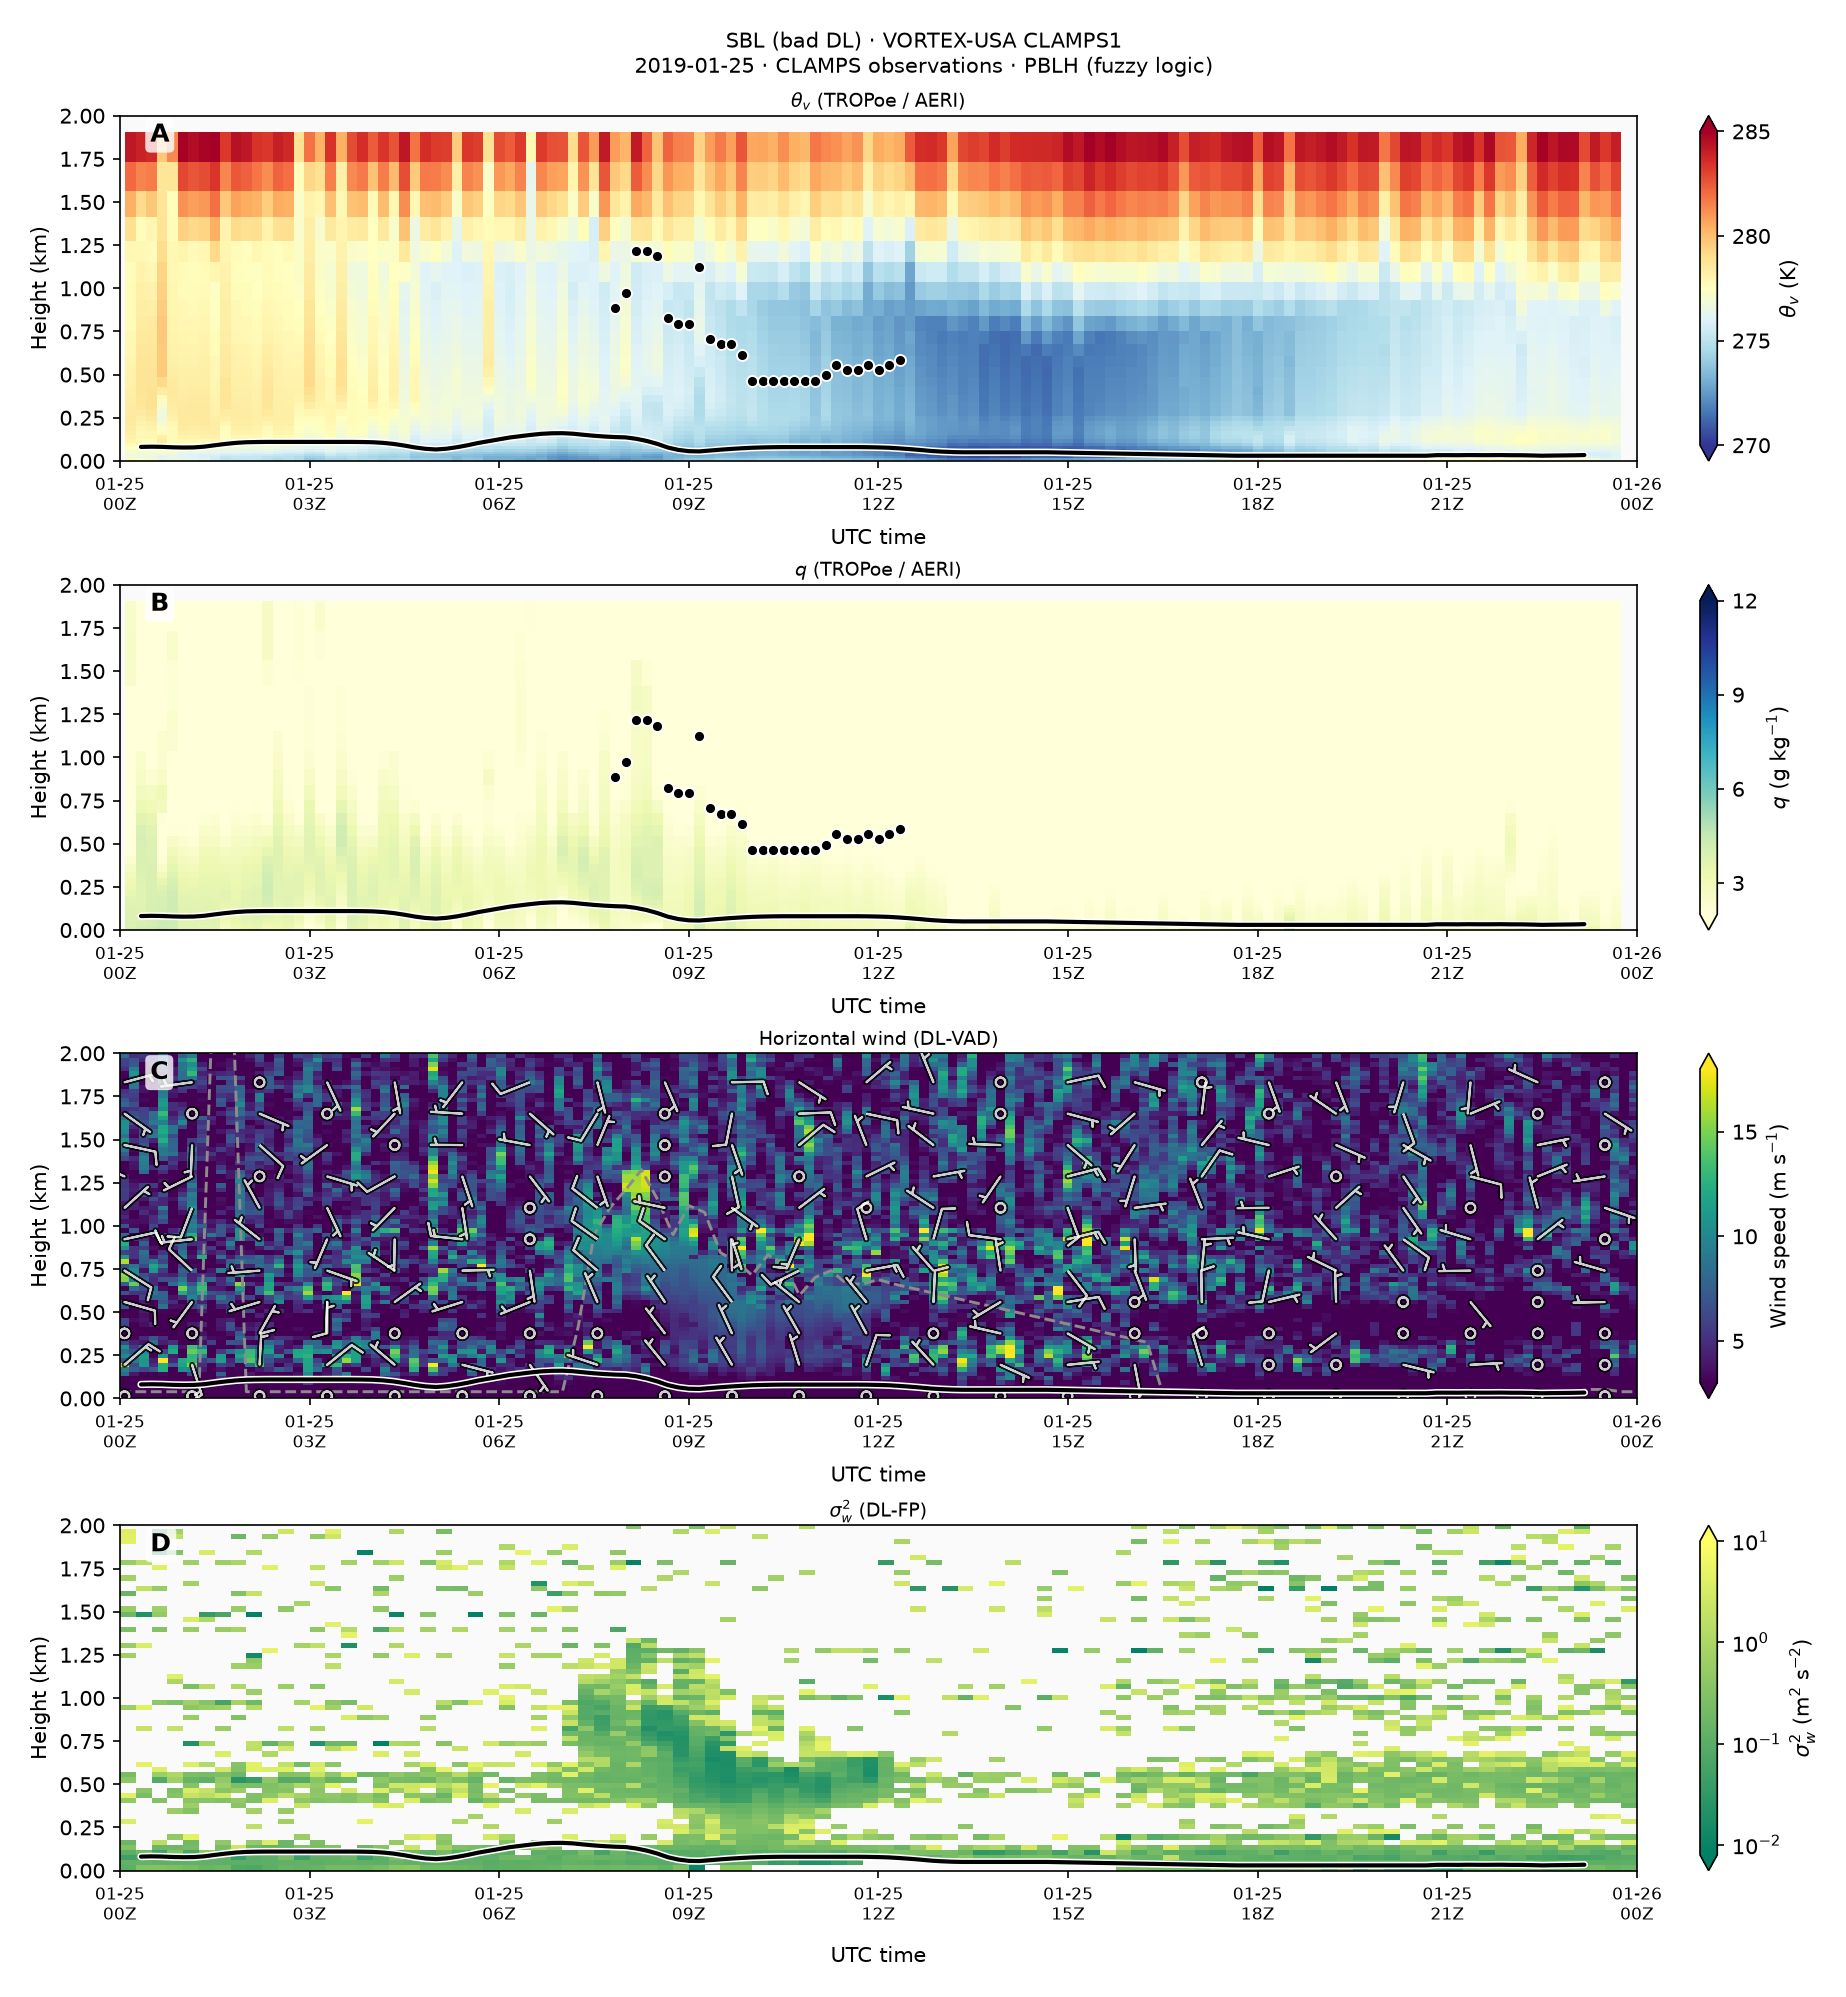
\includegraphics[width=\textwidth]{../../images/stable_bad_dl_c1_instrument_template_4panel.png}
  \caption{Standard CLAMPS observations.}
  \label{fig:stable_bad_dl_c1:stable_bad_dl_c1_instrument_template_4panel}
\end{figure}
\subsection*{Case overview}
This wintertime case illustrates a classic operational limitation of Doppler lidar systems within the CLAMPS platform. Following a cold or clean air mass passage, lidar observing can be limited under very low aerosol concentrations. Because Doppler lidars rely on atmospheric aerosols (such as dust, smoke, or pollution) to backscatter the transmitted laser pulse, a lack of particulate matter results in a low signal-to-noise ratio (SNR). Consequently, the lidar is unable to retrieve horizontal wind vectors or vertical velocity statistics across much of the column, despite the thermodynamic instruments continuing to capture the evolution of a cold, stable air mass.

\subsection*{Highlights}
\begin{itemize}
  \item Thermal Structure (Panel A): Unlike the summer cases, the virtual potential temperature ($\theta_v$) is extremely cold, hovering between 270 K and 280 K throughout the entire period. A persistent, shallow stable layer remains pinned beneath 150 m. Between 08:00 UTC and 14:00 UTC, a distinct elevated cooling event ($\theta_v < 272\text{ K}$, deep blue) descends from 1.25 km down to 0.5 km, marking a cold advection or frontal feature that the AERI/MWR thermodynamic retrievals successfully capture.
  \item Moisture Sublimation/Deficit (Panel B): Atmospheric moisture is exceptionally scarce, with specific humidity ($q$) flatlined near $1\text{ to }3\text{ g kg}^{-1}$ through the entire 2.0 km column. This extremely dry, cold continental air mass typically correlates with pristine, aerosol-poor air, independently verified by the surface weather logs in \hyperref[fig:stable_bad_dl_c1:stable_bad_dl_c1_aux_metar_meteogram]{METAR surface meteogram} which reveal an intensely clean post-frontal high-pressure system characterized by a building ridge (MSLP exceeding 1028 hPa) and unrestricted 10-mile visibility.
  \item Lidar Data Fragmentation \& Noise (Panel C): The horizontal wind plot (retrieved via DLVAD) shows a near-total failure of the retrieval algorithm. Outside of a small pocket around 07:00–10:00 UTC, the panel is dominated by random, unphysical speckle and chaotic wind barbs. This is a classic visual signature of the algorithm trying to process random atmospheric background noise because the actual laser backscatter signal has fallen below the instrument's detection threshold, as explicitly proven by the raw signal strength plunging below $-20\text{ dB}$ across the gray noise regions of \hyperref[fig:stable_bad_dl_c1:stable_bad_dl_c1_aux_dlfp_snr_timeheight]{DL-FP SNR time–height}.
  \item Vertical Velocity Variance Dropouts (Panel D): The $\sigma_w^2$ panel similarly reveals severe data fragmentation. While a brief plume of turbulent variance is resolved between 07:00 UTC and 11:00 UTC (coinciding with the shifting feature seen in the temperature profile), the rest of the 24-hour period is largely blank or speckled with unphysical noise. This total loss of vertical velocity tracking maps perfectly to \hyperref[fig:stable_bad_dl_c1:stable_bad_dl_c1_aux_dlfp_snr_timeheight]{DL-FP SNR time–height}, demonstrating that valid kinematic data collection only occurs when the localized elevated aerosol plume briefly hoists the Lidar SNR back above the detection floor.
\end{itemize}
\begin{figure}[htbp]
  \centering
  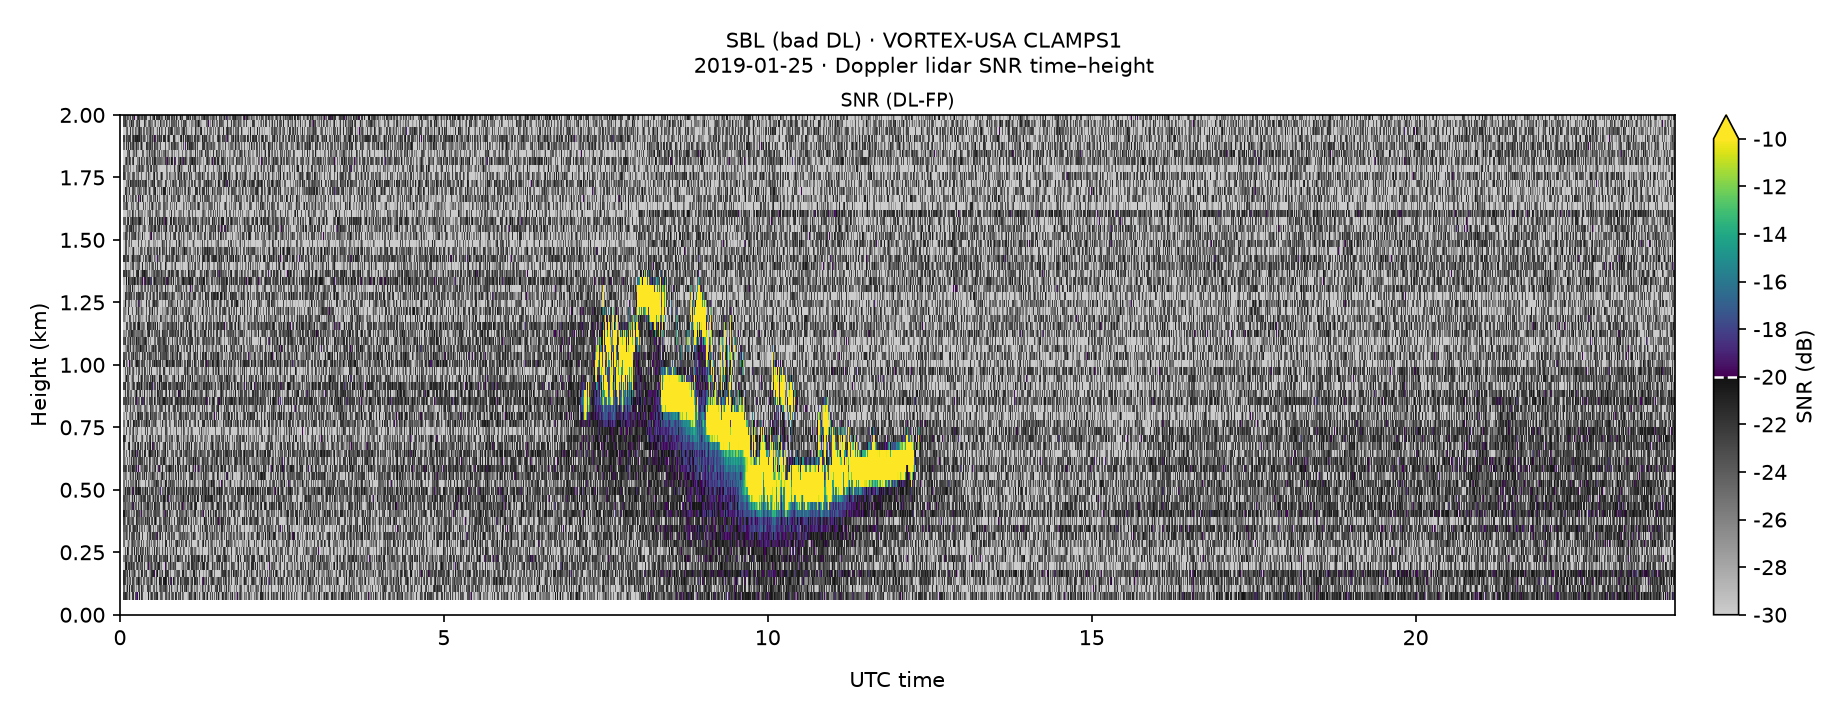
\includegraphics[width=0.92\textwidth]{../../images/stable_bad_dl_c1_aux_dlfp_snr_timeheight.png}
  \caption{DL-FP SNR time–height.
  DL-FP signal-to-noise ratio ($\mathrm{SNR}+1$) time–height. Gray regions below the detection threshold correspond to periods when kinematic retrievals fail in aerosol-poor air.}
  \label{fig:stable_bad_dl_c1:stable_bad_dl_c1_aux_dlfp_snr_timeheight}
\end{figure}
\begin{figure}[htbp]
  \centering
  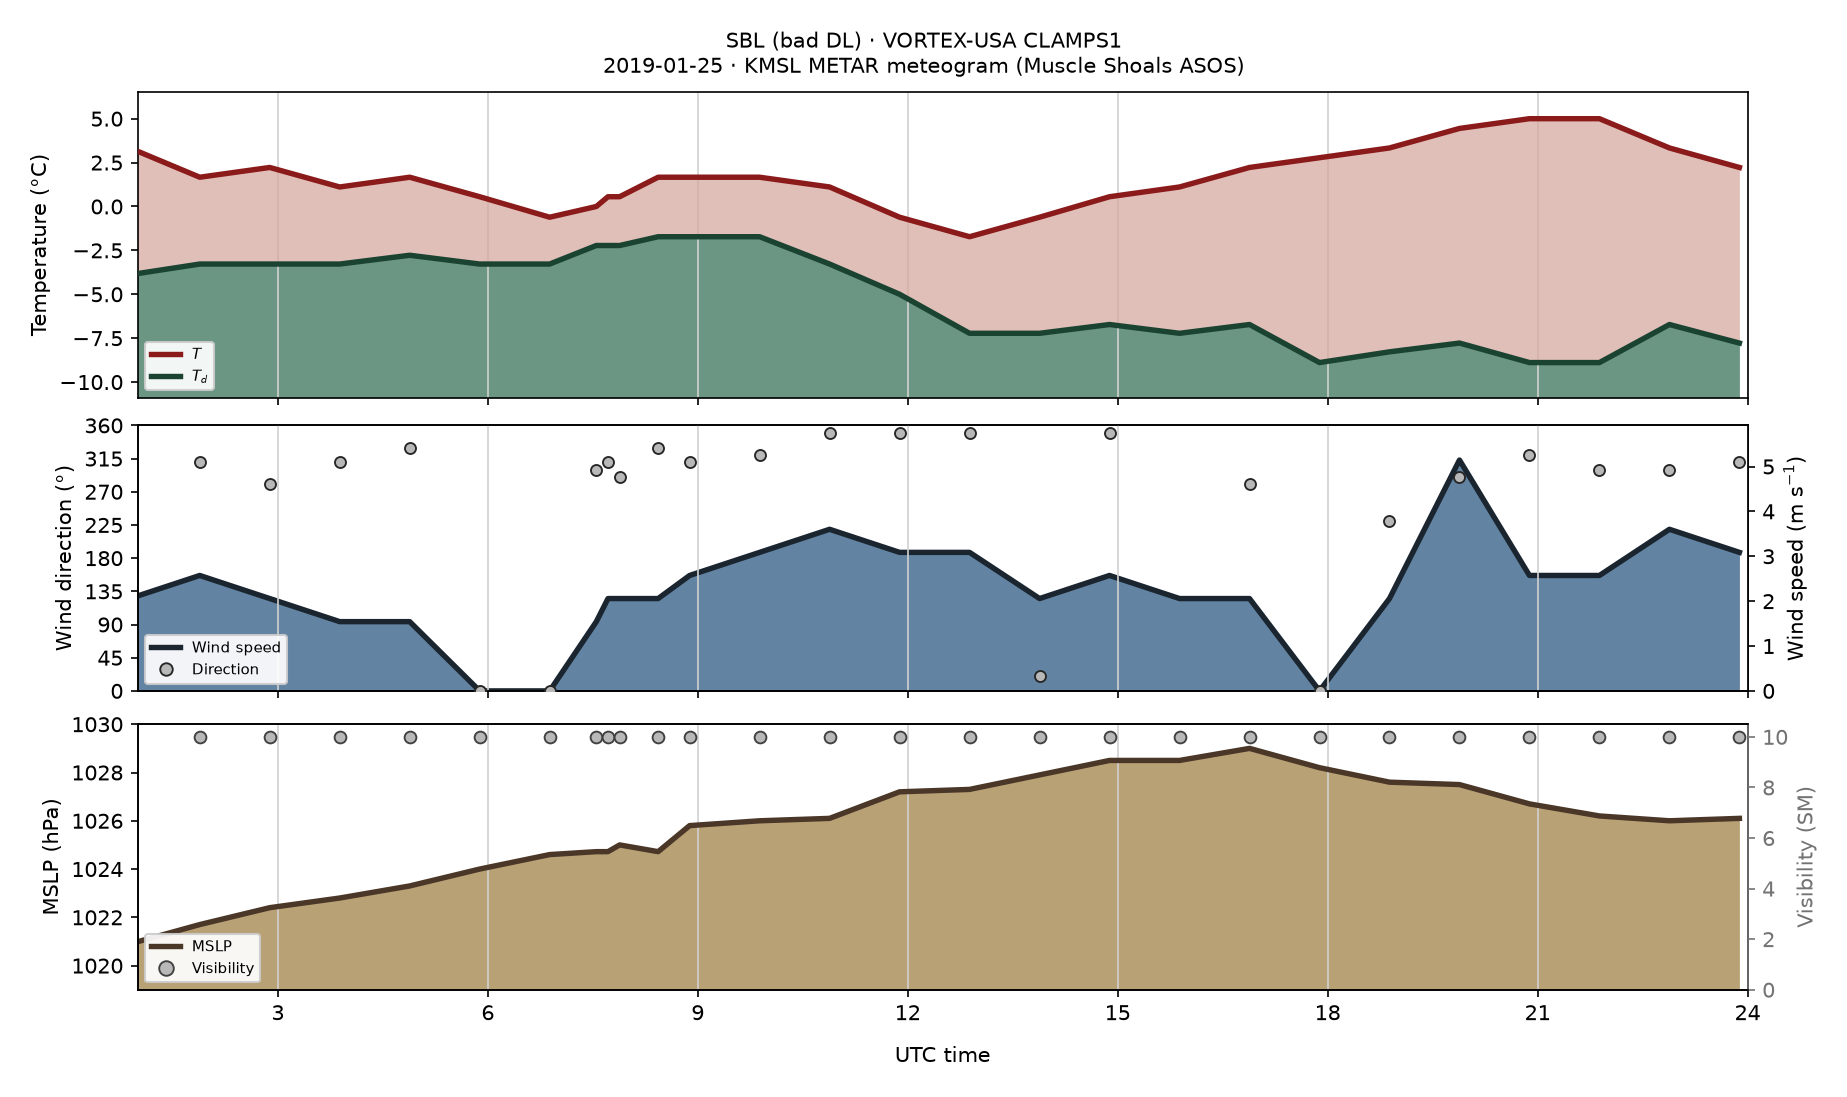
\includegraphics[width=0.92\textwidth]{../../images/stable_bad_dl_c1_aux_metar_meteogram.png}
  \caption{METAR surface meteogram.
  METAR surface observations documenting the intensely clean post-frontal high-pressure regime (MSLP $> 1028$ hPa) and unrestricted visibility characteristic of aerosol-depleted winter air masses.}
  \label{fig:stable_bad_dl_c1:stable_bad_dl_c1_aux_metar_meteogram}
\end{figure}
\section{Convection Initiation \& Gravity Waves}
\textit{CLAMPS1 $\cdot$ NWCRIL 2020 $\cdot$ Norman, OK $\cdot$ July 30, 2020 $\cdot$ convection, CI, gravity waves, boundaries, bore}

\begin{figure}[htbp]
  \centering
  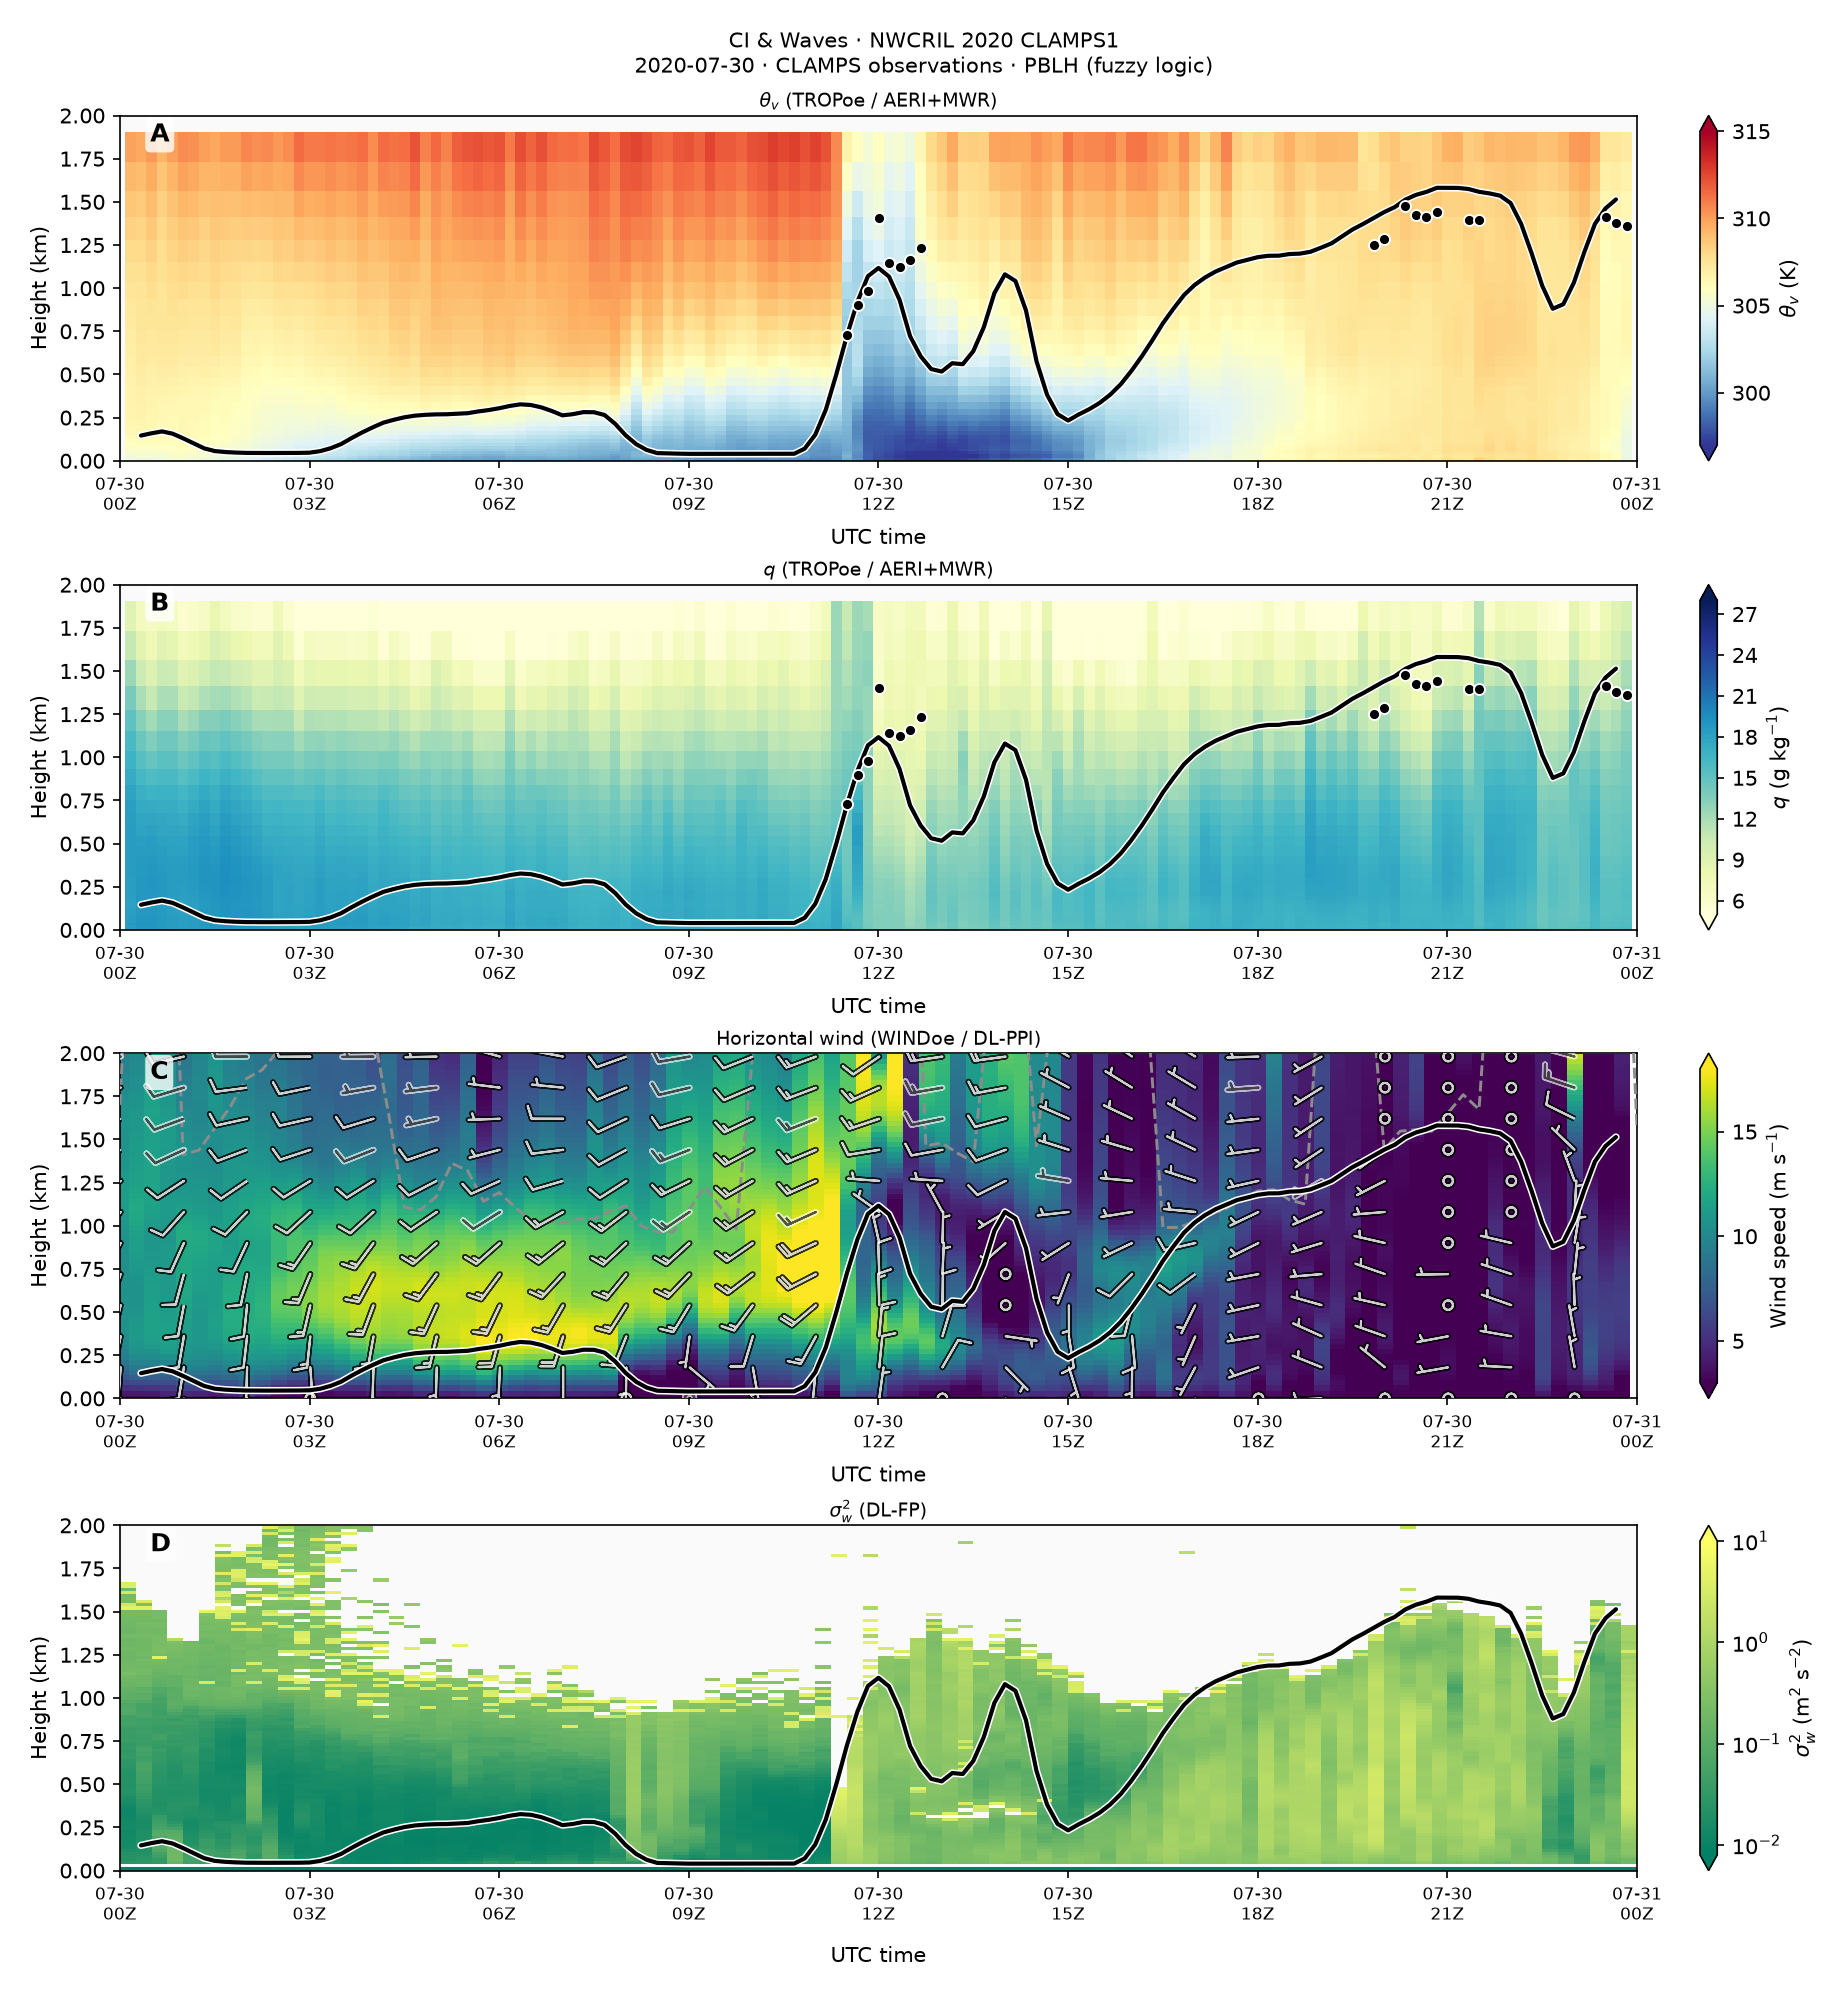
\includegraphics[width=\textwidth]{../../images/ci_c1_instrument_template_4panel.png}
  \caption{Standard CLAMPS observations.}
  \label{fig:ci_gravity_waves_c1:ci_c1_instrument_template_4panel}
\end{figure}
\subsection*{Case overview}
This case captures the complex interaction between a nocturnal low-level jet, wave dynamics, and subsequent convection initiation (CI). Prior to 11:00 UTC, a well-defined NLLJ dominates the lower kilometer. Around 11:00 UTC, an incoming mesoscale disturbance abruptly disrupts the jet. This interaction excites a classic atmospheric bore visible as massive, periodic vertical undulations in the thermodynamic and moisture fields between 11:00 and 16:00 UTC. The intense, localized vertical lifting supplied by these waves successfully hoists a deep layer of low-level moisture past the capping inversion, destabilizing the environment and triggering deep convection later in the period.

\subsection*{Highlights}
\begin{itemize}
  \item Dramatic Wave Undulations (Panel A): Between 11:00 UTC and 16:00 UTC, the virtual potential temperature ($\theta_v$) profiles in \hyperref[fig:ci_gravity_waves_c1:ci_c1_instrument_template_4panel]{Standard CLAMPS observations} reveal a spectacular undulating wave structure. The fuzzy-logic boundary layer height (PBLH) line oscillates violently, tracking a massive initial crest up to 1.1 km at 12:00 UTC, dropping into a trough at 13:00 UTC, and surging back to 1.1 km at 14:00 UTC. This periodic lifting and dropping is further resolved as a coherent gravity wave train with intense alternating updraft and downdraft cores exceeding $\pm 2\text{ m s}^{-1}$ in the high-frequency vertical velocity zoom of \hyperref[fig:ci_gravity_waves_c1:ci_c1_aux_dlfp_w_zoom_timeheight]{DL-FP vertical velocity zoom}.
  \item The Moisture Pump (Panel B): Prior to the wave's arrival, an incredibly rich reservoir of moisture ($q \approx 15\text{ to }18\text{ g kg}^{-1}$) is confined below 1.0 km in \hyperref[fig:ci_gravity_waves_c1:ci_c1_instrument_template_4panel]{Standard CLAMPS observations}. As the wave train passes, it acts as a mechanical pump, physically hoisting this deep moisture layer upward by more than 1 km during the wave crests. This substantial vertical displacement is critical for breaching the nocturnal capping inversion to initiate convection.
  \item Jet Termination, Wind Shift, \& Surface Signature (Panel C): A strong NLLJ with horizontal wind speeds exceeding $15\text{ m s}^{-1}$ is active from 02:00 to 11:00 UTC. Right at 11:20 UTC, the jet is abruptly sheared and terminated by the arriving boundary. The surface meteogram in \hyperref[fig:ci_gravity_waves_c1:ci_c1_aux_surface_meteogram]{Surface meteogram (CLAMPS1)} diagnoses this arrival as a true physical bore/density current, recording a violent 3 hPa surface pressure jump, an abrupt wind shift, and an instantaneous wind speed spike up to 10 m/s. The regional tracking of this outrunning convective boundary as it marches directly over the Norman platform is confirmed via the KTLX NEXRAD radar loop in \hyperref[fig:ci_gravity_waves_c1:ci_c1_20200730_88dloop]{NEXRAD 88D reflectivity loop}.
  \item Wave-Induced Turbulence \& Storm Growth (Panel D): The Doppler Lidar vertical velocity variance ($\sigma_w^2$) transitions from a stratified, quiet nocturnal regime to showing distinct bursts of enhanced turbulence that align perfectly with the wave crests. After 16:00 UTC, the widespread, intense variance throughout the entire 2.0 km column marks the realization of deep convective mixing and storm development following successful convection initiation.
\end{itemize}
\begin{figure}[htbp]
  \centering
  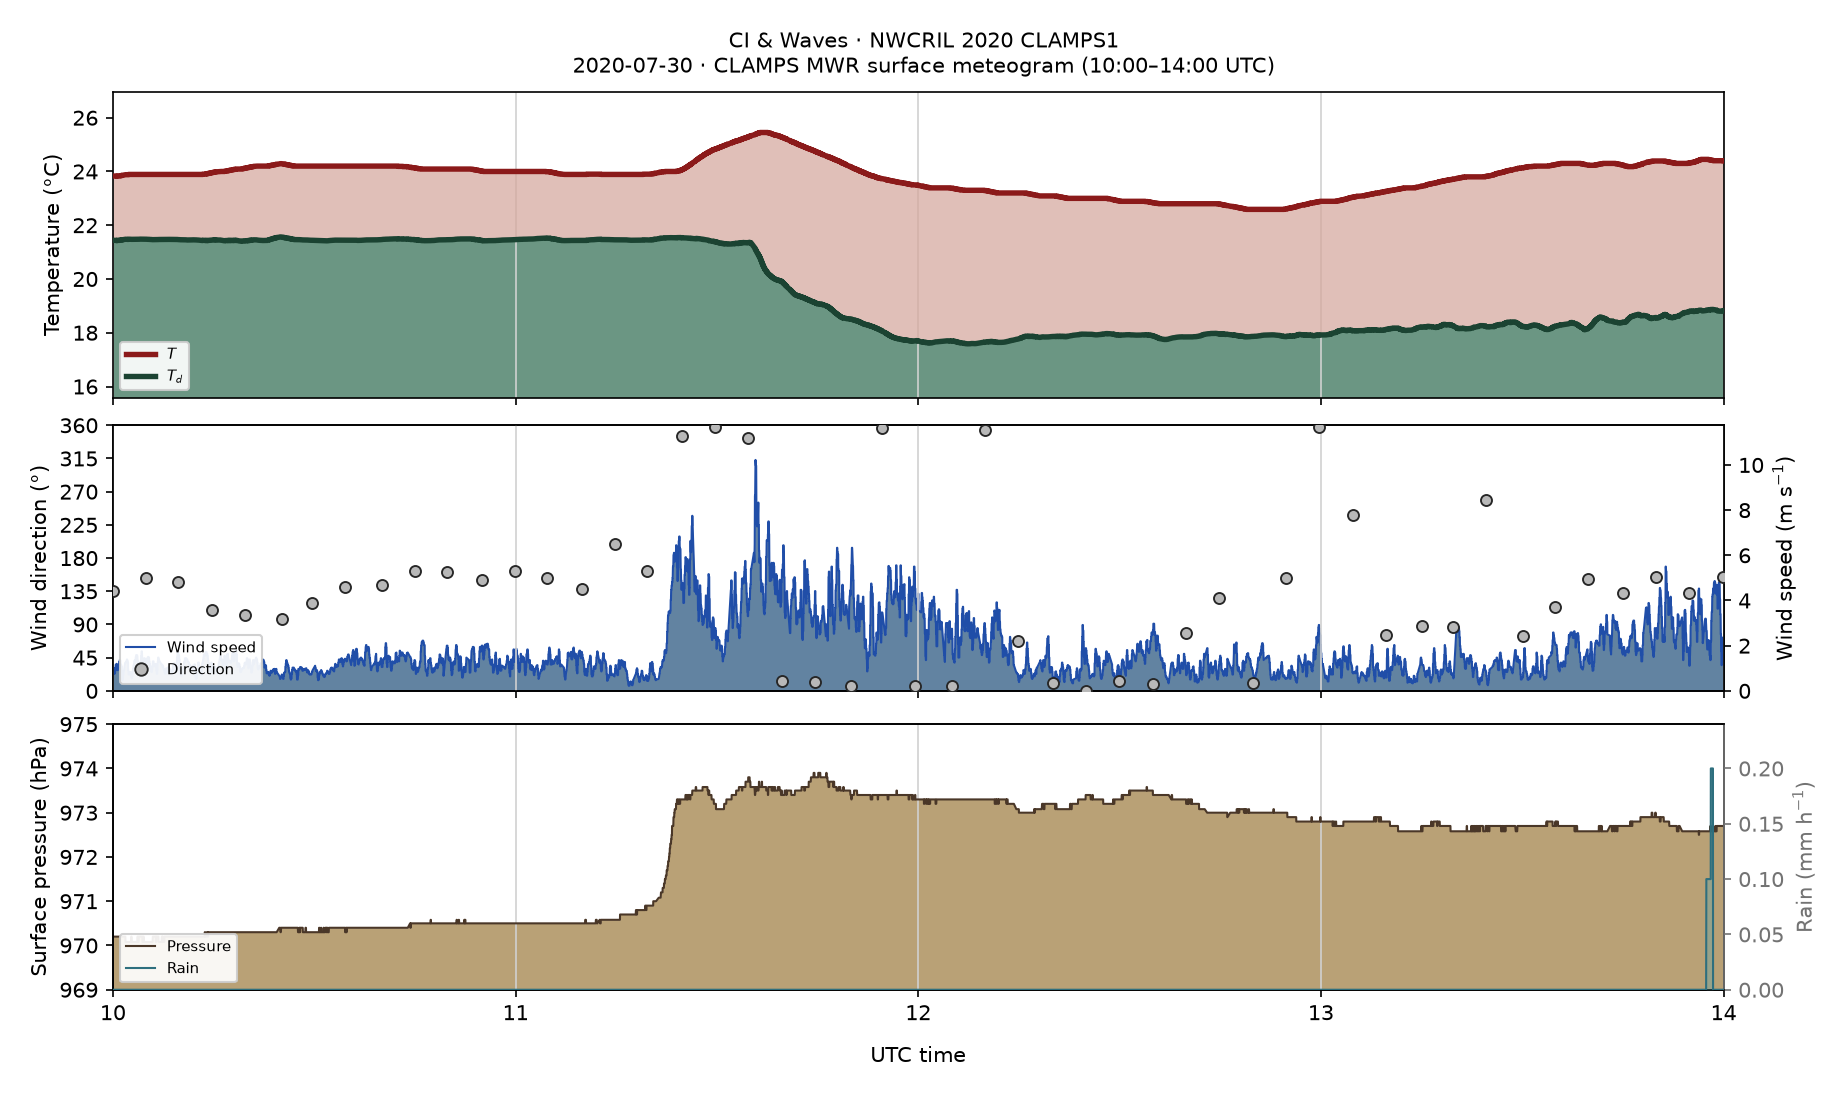
\includegraphics[width=0.92\textwidth]{../../images/ci_c1_aux_surface_meteogram.png}
  \caption{Surface meteogram (CLAMPS1).
  CLAMPS1 surface pressure, wind, temperature, and humidity time series diagnosing the bore arrival at 11:20 UTC via hydrostatic pressure jump, wind shift, and gust spike.}
  \label{fig:ci_gravity_waves_c1:ci_c1_aux_surface_meteogram}
\end{figure}
\begin{figure}[htbp]
  \centering
  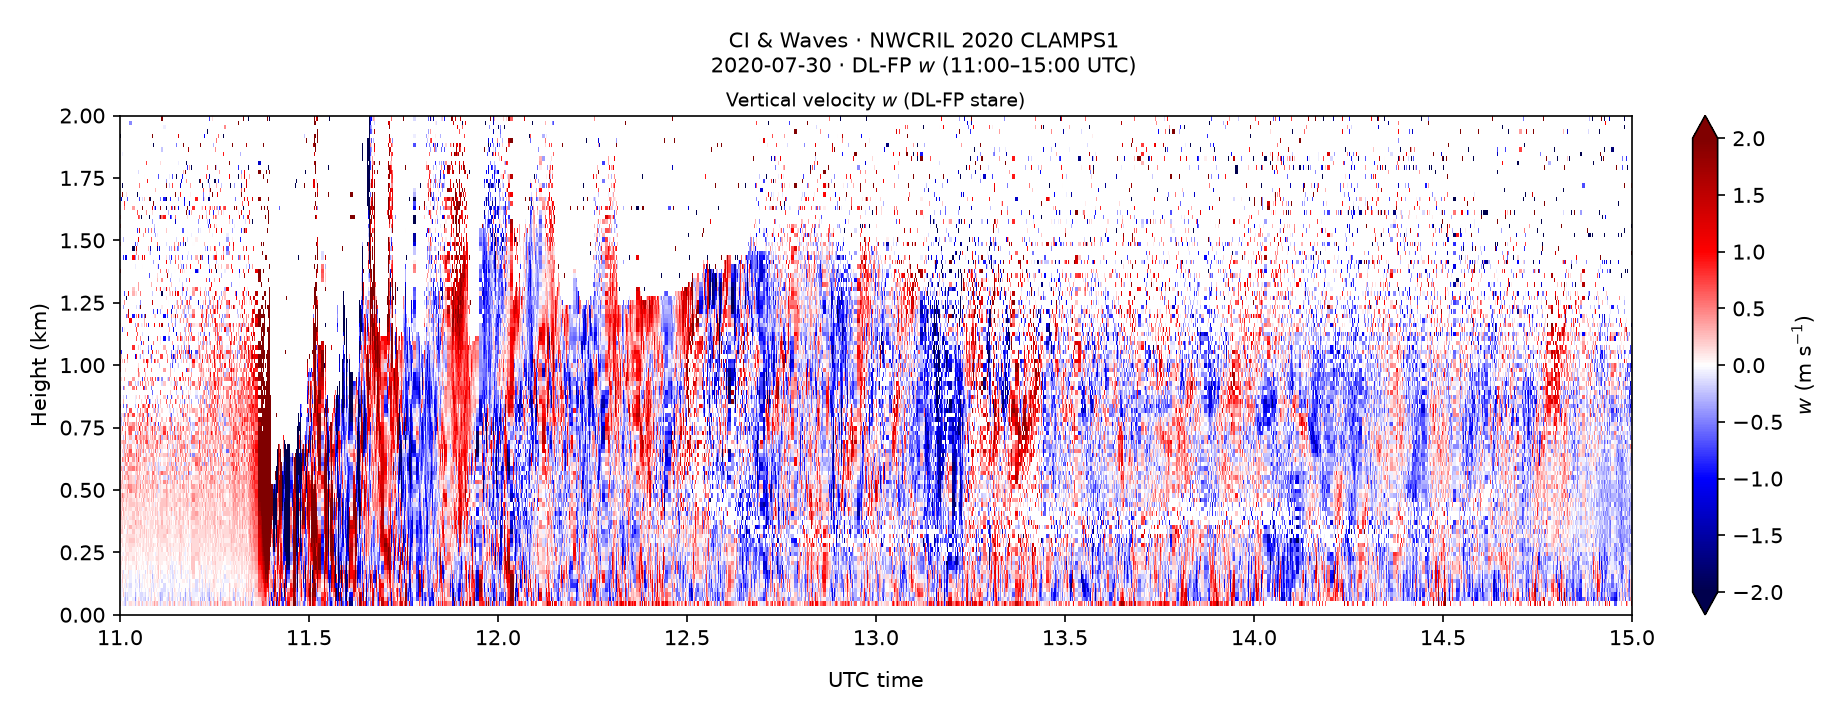
\includegraphics[width=0.92\textwidth]{../../images/ci_c1_aux_dlfp_w_zoom_timeheight.png}
  \caption{DL-FP vertical velocity zoom.
  High-resolution DL-FP vertical velocity during the 11:00–16:00 UTC gravity wave train, revealing coherent updraft and downdraft cores exceeding $\pm 2\,\mathrm{m\,s^{-1}}$.}
  \label{fig:ci_gravity_waves_c1:ci_c1_aux_dlfp_w_zoom_timeheight}
\end{figure}
\begin{figure}[htbp]
  \centering
  \includegraphics[width=0.92\textwidth]{_frames/ci_c1_20200730_88Dloop.png}
  \caption{NEXRAD 88D reflectivity loop.
  KTLX WSR-88D reflectivity loop tracking the convective outflow boundary marching eastward over the Norman platform. First frame of animated loop; full animation available in the online gallery.}
  \label{fig:ci_gravity_waves_c1:ci_c1_20200730_88dloop}
\end{figure}
\section{Diurnal Cycle}
\textit{CLAMPS2 $\cdot$ BLISSFUL $\cdot$ Washington, OK $\cdot$ July 6, 2021 $\cdot$ diurnal, boundary layer, CBL}

\begin{figure}[htbp]
  \centering
  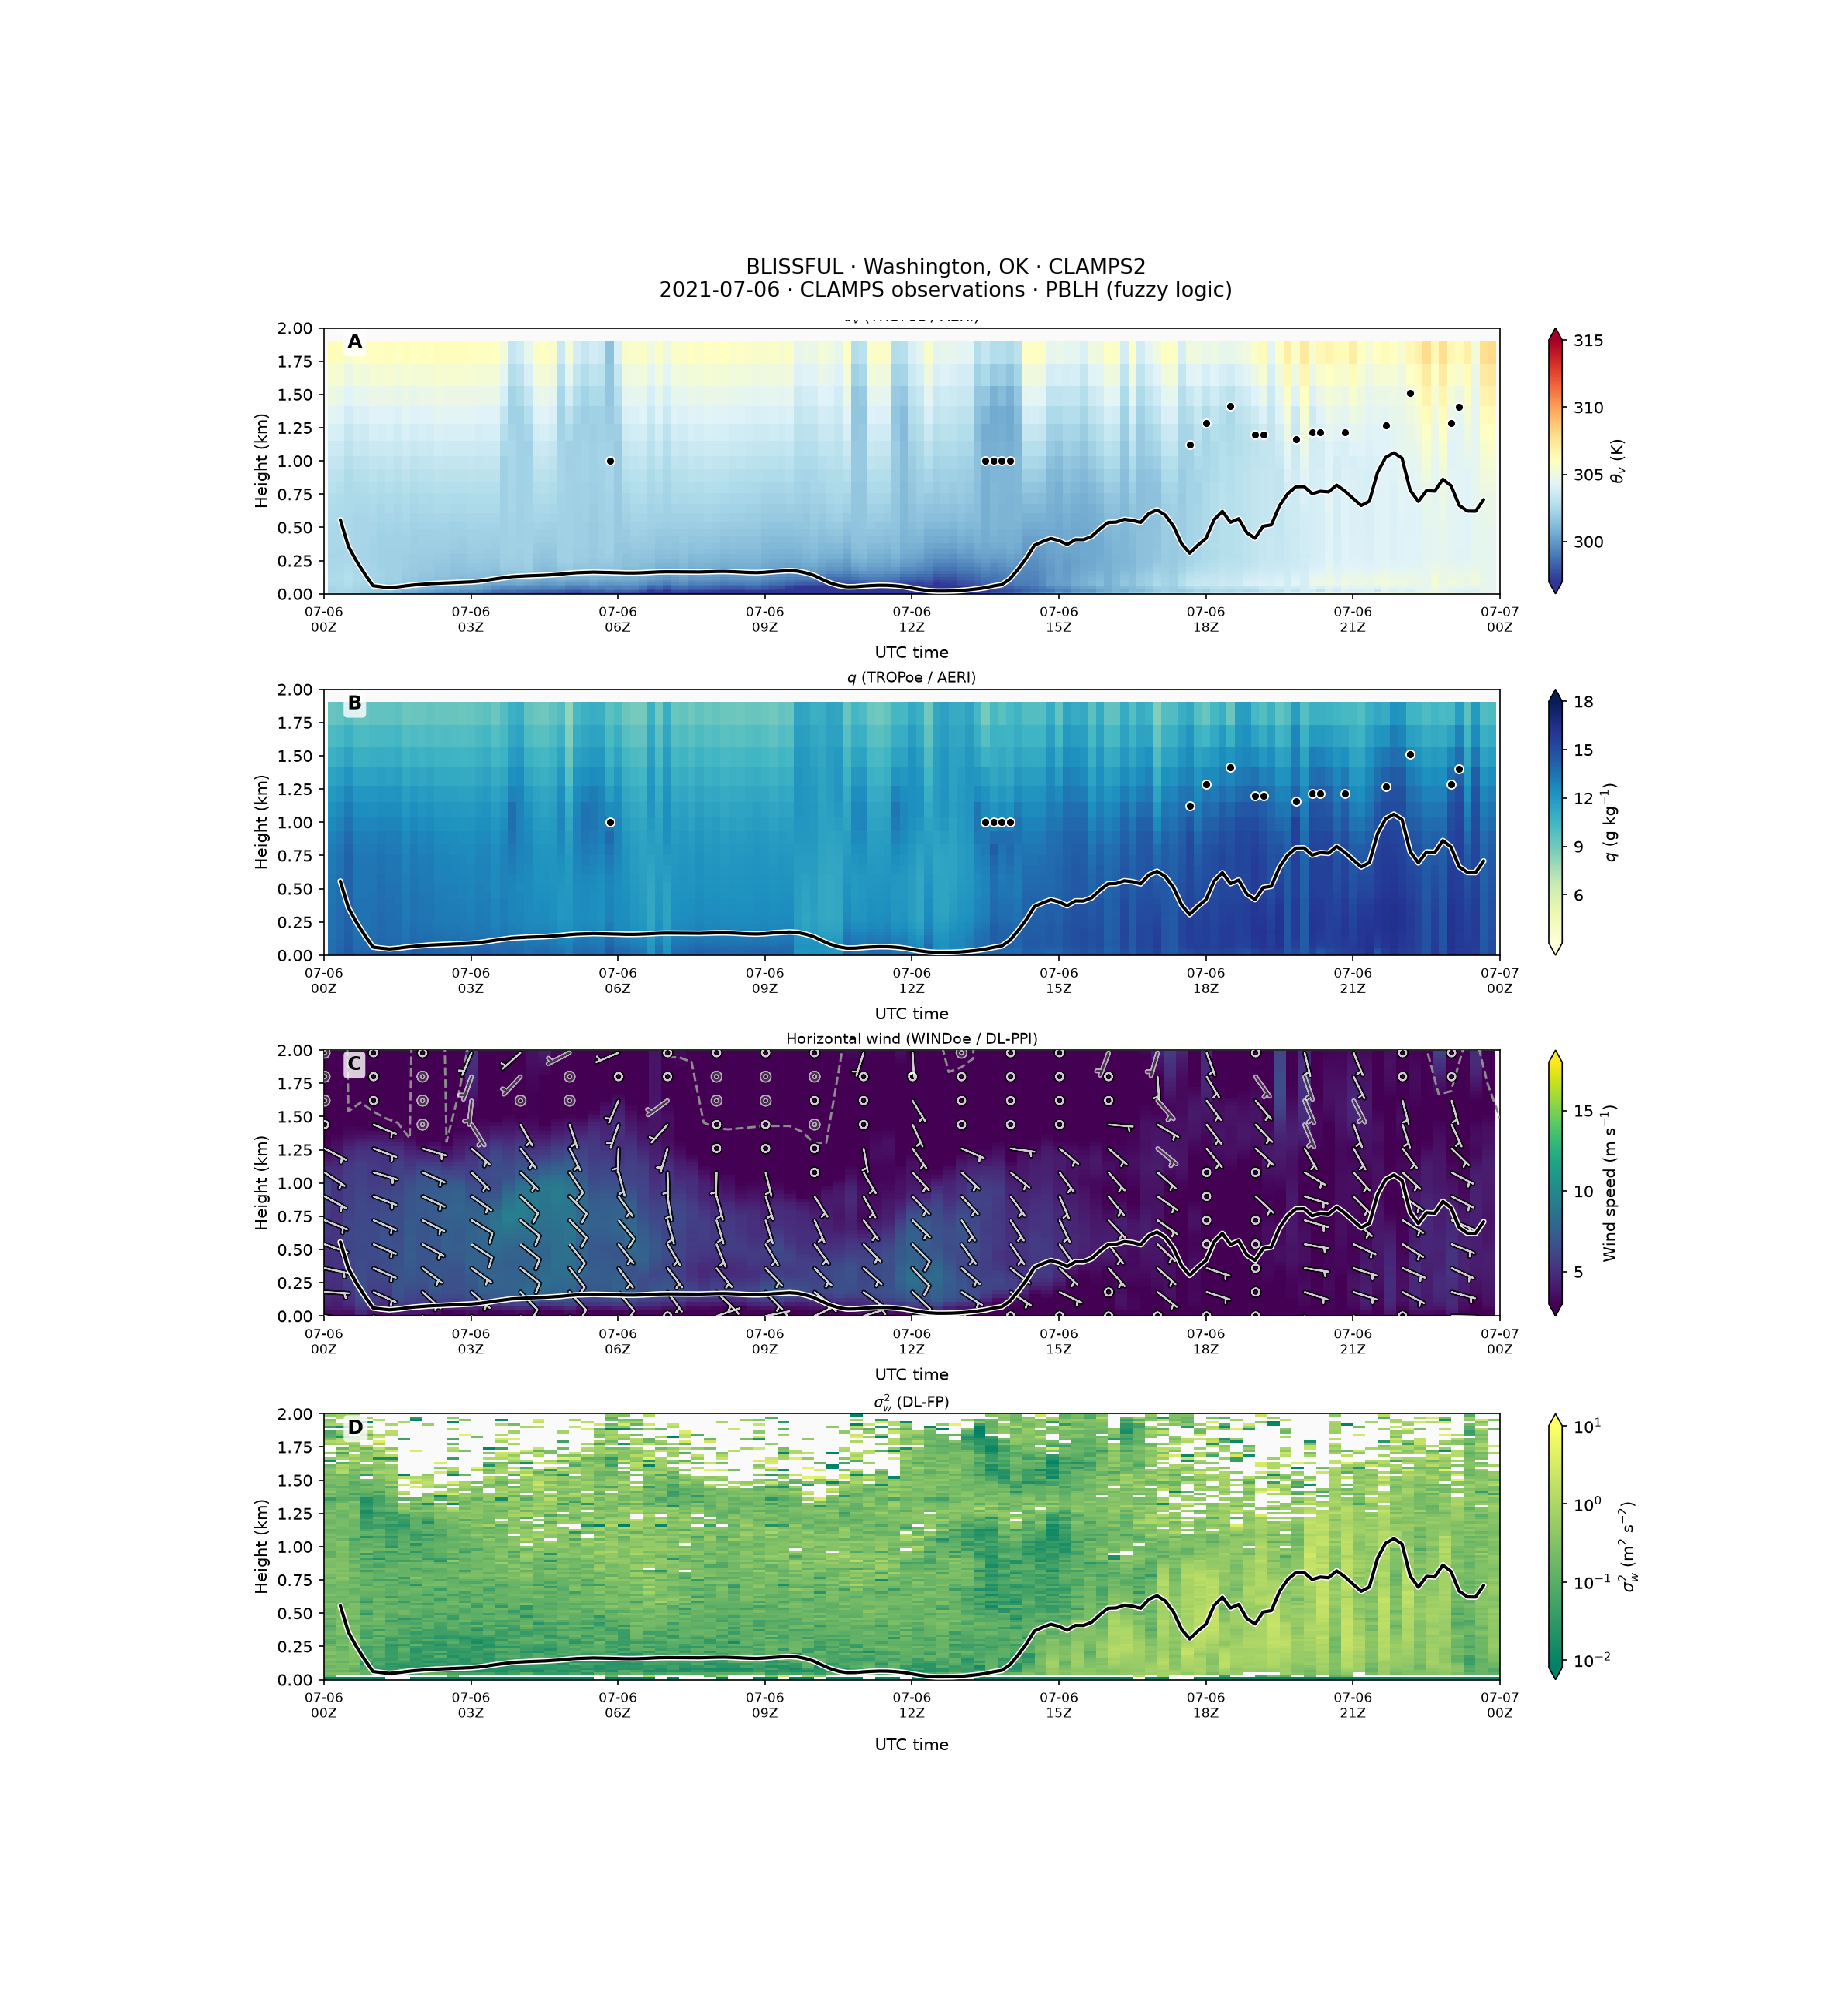
\includegraphics[width=\textwidth]{../../images/diurnal_c2_instrument_template_4panel.png}
  \caption{Standard CLAMPS observations.}
  \label{fig:diurnal_c2:diurnal_c2_instrument_template_4panel}
\end{figure}
\subsection*{Case overview}
This 30-hour case study captures a highly complex diurnal boundary layer cycle observed by CLAMPS2 during the BLISSFUL campaign, extending from 00:00 UTC on July 6 to 06:00 UTC on July 7, 2021. The standard afternoon convective boundary layer (CBL) growth is significantly disrupted during the evening transition by nearby convective activity. Rather than undergoing a clean, progressive stabilization at sunset (\textasciitilde{}01:00 UTC), the boundary layer interacts with an incoming convective outflow boundary at approximately 23:30 UTC. This mesoscale feature forces a deep vertical ascent that mechanically rejuvenates turbulent mixing right at sunset. The subsequent nocturnal period is characterized by a delayed shutdown of surface-based eddies and prominent, periodic gravity-wave-like undulations trapped within the residual layer.

\subsection*{Highlights}
\begin{itemize}
  \item Daytime Convection \& Cloud Cover (18:00–22:00 UTC) [Panel A \& B]: Strong solar insulation drives a deep mixed layer with virtual potential temperatures ($\theta_v$) reaching 310 to 312 K in panel A of \hyperref[fig:diurnal_c2:diurnal_c2_instrument_template_4panel]{Standard CLAMPS observations}. Automated retrieval algorithms flag a series of cloud bases between 1.25 km and 1.5 km (black scatter points), matching the fully expanded planetary boundary layer height (PBLH) tracking line.
  \item Convective Outflow \& Forced Ascent (\textasciitilde{}23:30 UTC): Right before sunset, a sharp mesoscale boundary impacts the site. This event is marked by a sudden structural shift in $\theta_v$ and moisture alongside an abrupt wind vector change in panel C of \hyperref[fig:diurnal_c2:diurnal_c2_instrument_template_4panel]{Standard CLAMPS observations}. The underlying surface-level response is captured in fine detail by the high-frequency time-series of \hyperref[fig:diurnal_c2:diurnal_c2_aux_surface_meteogram]{Surface meteogram}, which documents a sudden temperature drop, wind speed spike, and distinct hydrostatic pressure jump.
  \item Reinvigorated Mixing \& Delayed Sunset Shutdown (00:00–03:00 UTC): While solar forcing diminishes around 01:00 UTC, the boundary passage mechanically rejuvenates turbulent mixing. Panel D of \hyperref[fig:diurnal_c2:diurnal_c2_instrument_template_4panel]{Standard CLAMPS observations} shows that vertical velocity variance ($\sigma_w^2$) remains elevated deep into the evening—a multi-stage transition mapped out clearly in the annotated staring scan of \hyperref[fig:diurnal_c2:diurnal_c2_clamps2stare]{DL-FP vertical stare} as a post-boundary burst of mixing followed by a gradual decay of surface-based eddies extending past 03:00 UTC.
  \item Nocturnal Wave Features \& Intermittent Turbulence (01:00–06:00 UTC): Once the surface fully decouples, the stable nocturnal boundary layer locks in near the ground ($<250\text{ m}$). However, the upper boundary layer remains highly dynamic. Panel D of \hyperref[fig:diurnal_c2:diurnal_c2_instrument_template_4panel]{Standard CLAMPS observations} displays persistent bands of elevated variance aloft, which are mathematically identified as low-stability, shear-driven zones ($Ri_b < 0.25$) in the Bulk Richardson number cross-section of \hyperref[fig:diurnal_c2:diurnal_c2_aux_rib_timeheight]{Bulk Richardson number time–height}.
  \item Forced Updraft Core (\textasciitilde{}23:30 UTC): The immediate kinematic footprint of the outflow boundary's arrival is explicitly exposed in the raw vertical velocity scan of \hyperref[fig:diurnal_c2:diurnal_c2_clamps2stare]{DL-FP vertical stare} as a narrow, highly intense column of deep vertical ascent with upward velocities exceeding 1 to 2 $\text{m s}^{-1}$ (dark red vertical strip).
  \item Trapped Residual Layer Waves (00:00–06:00 UTC): Above the shallow nocturnal surface layer ($<250$ m), the continuous, long-period wave train annotated in \hyperref[fig:diurnal_c2:diurnal_c2_clamps2stare]{DL-FP vertical stare} beautifully captures trapped gravity waves rippling through the stable residual layer column.
  \item Thermodynamic Retrieval Validation: Co-located radiosonde comparisons in \hyperref[fig:diurnal_c2:diurnal_c2_aux_skewt_overlay]{Skew-T overlay (radiosonde comparison)} at 20:24 and 22:20 UTC verify the high accuracy of the TROPoe profiles throughout the lower boundary layer (1000 to 700 hPa), capturing the deeply mixed, dry-adiabatic afternoon structure and demonstrating the smooth vertical filtering characteristic of ground-based remote sensing instruments.
\end{itemize}
\begin{figure}[htbp]
  \centering
  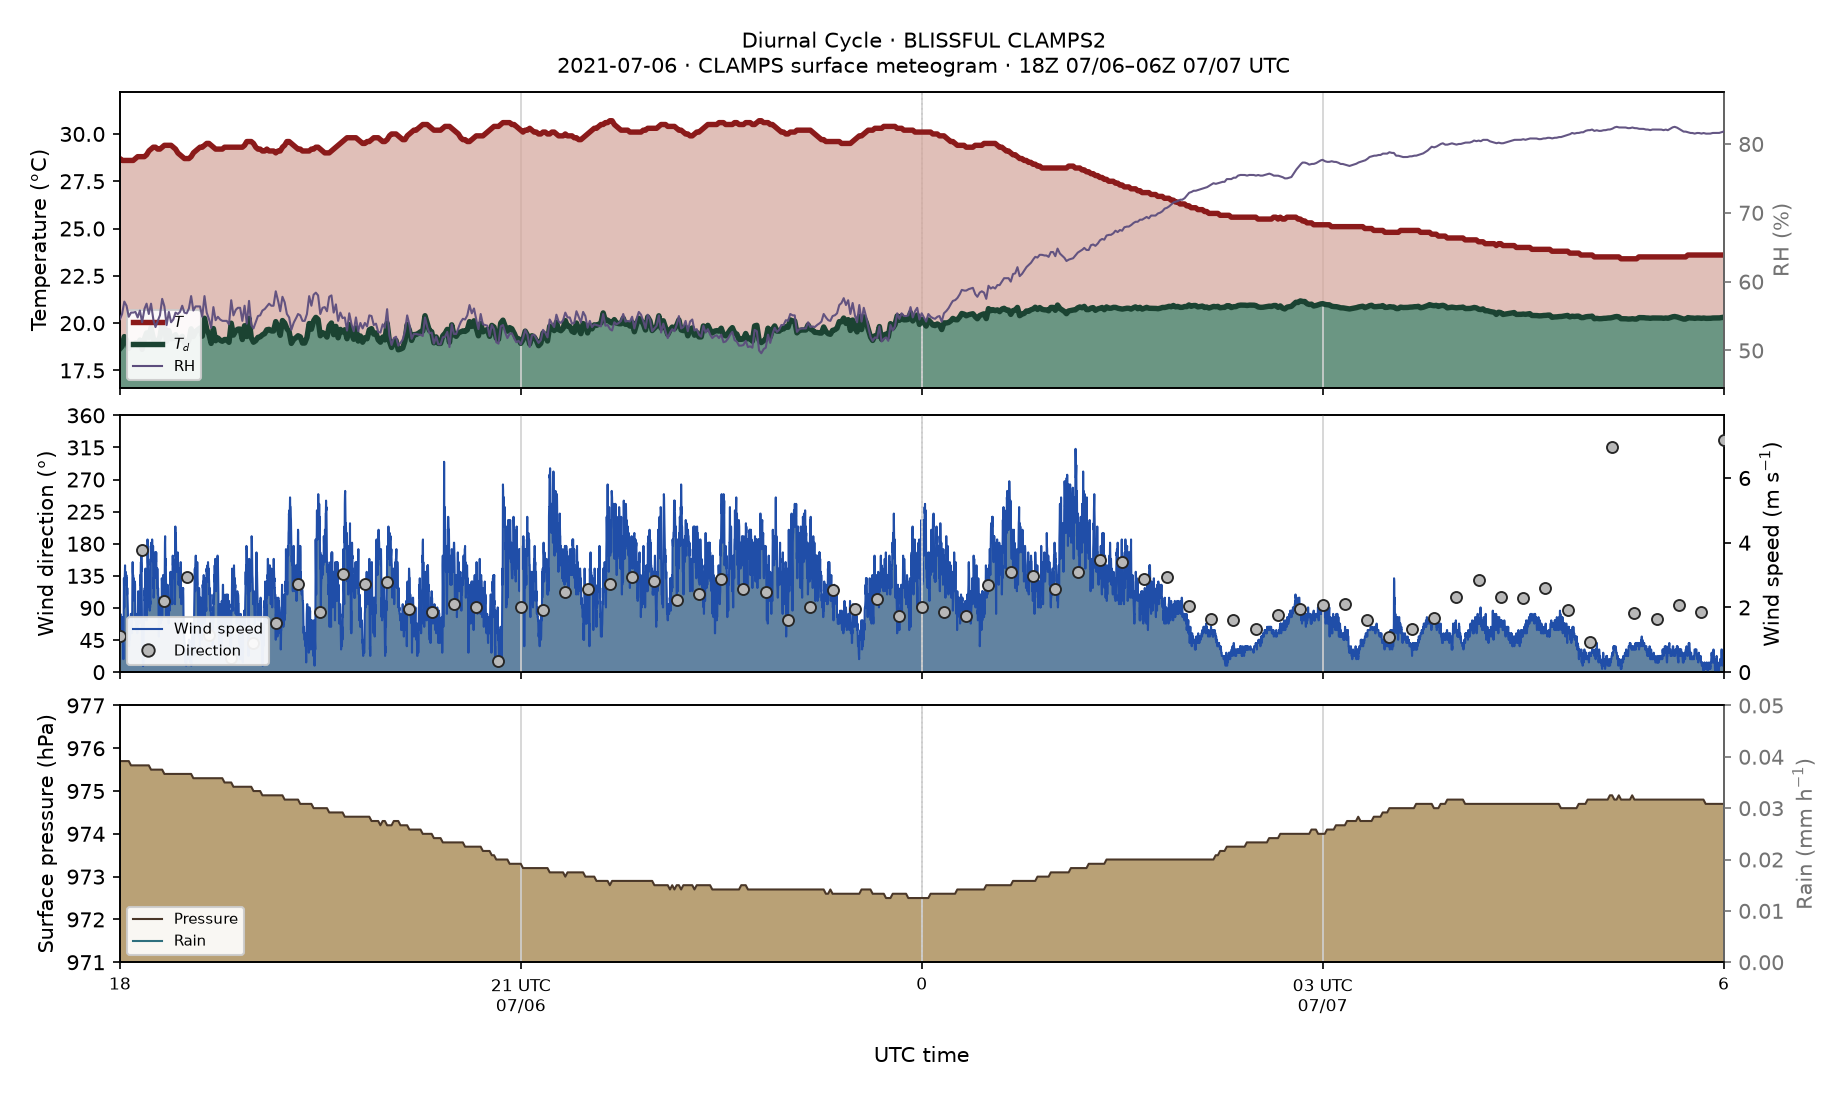
\includegraphics[width=0.92\textwidth]{../../images/diurnal_c2_aux_surface_meteogram.png}
  \caption{Surface meteogram.
  High-cadence surface meteogram capturing the convective outflow pressure jump, temperature drop, and wind spike at $\sim$23:30 UTC.}
  \label{fig:diurnal_c2:diurnal_c2_aux_surface_meteogram}
\end{figure}
\begin{figure}[htbp]
  \centering
  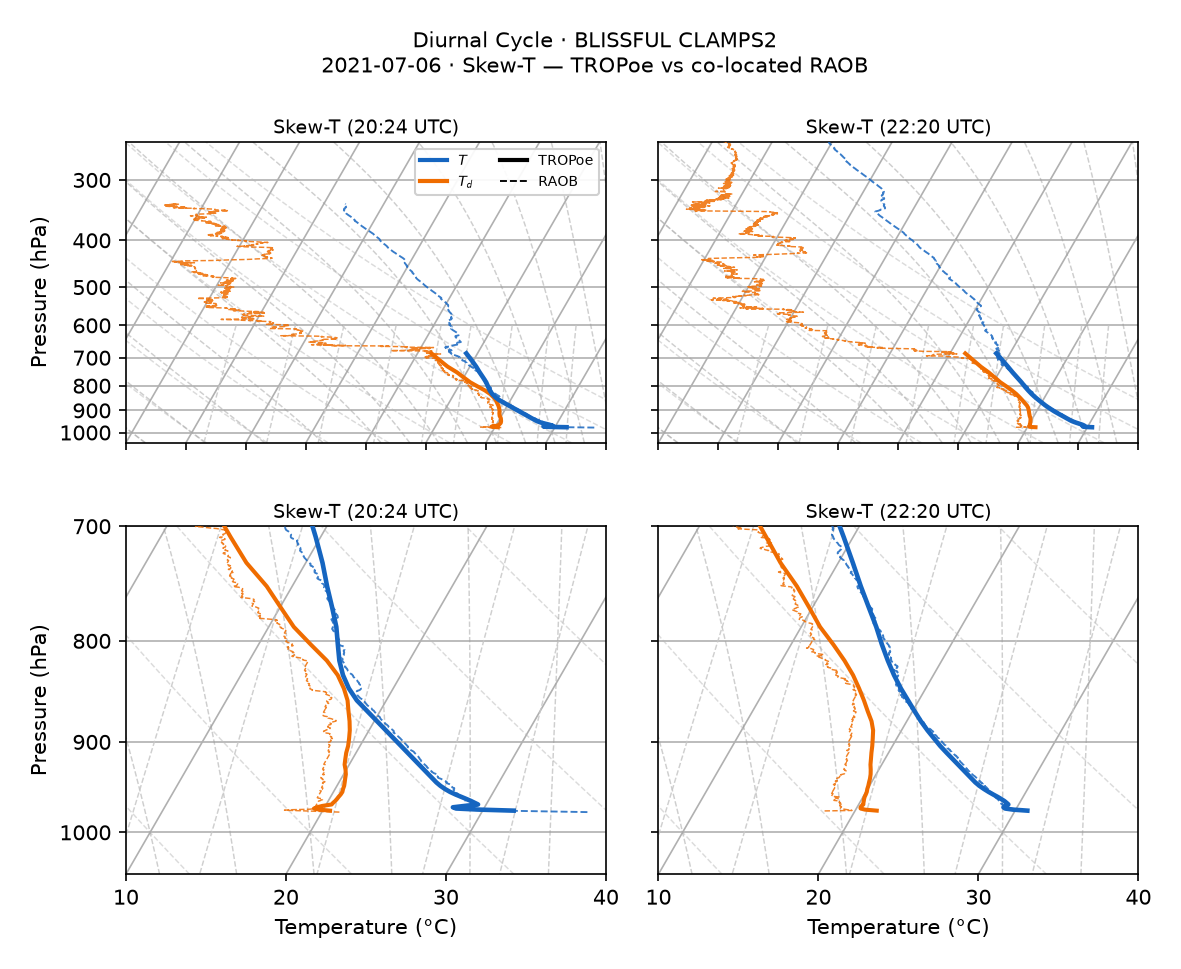
\includegraphics[width=0.92\textwidth]{../../images/diurnal_c2_aux_skewt_overlay.png}
  \caption{Skew-T overlay (radiosonde comparison).
  TROPoe thermodynamic profiles compared with co-located radiosonde soundings at 20:24 and 22:20 UTC, validating retrieval accuracy through the afternoon mixed layer.}
  \label{fig:diurnal_c2:diurnal_c2_aux_skewt_overlay}
\end{figure}
\begin{figure}[htbp]
  \centering
  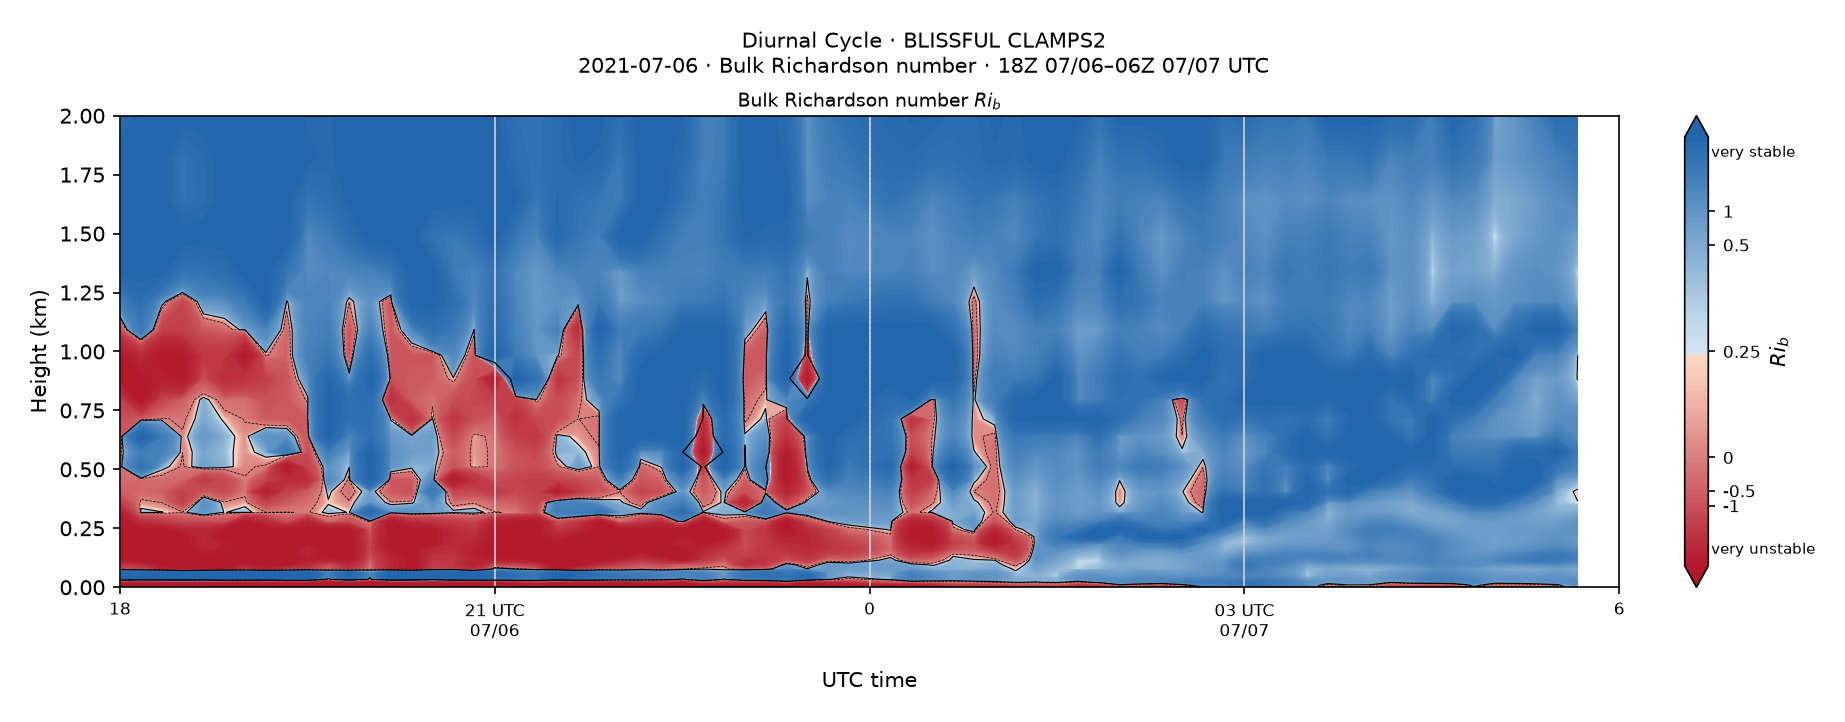
\includegraphics[width=0.92\textwidth]{../../images/diurnal_c2_aux_rib_timeheight.png}
  \caption{Bulk Richardson number time–height.
  Bulk Richardson number $Ri_b$ time–height cross-section identifying shear-driven unstable layers ($Ri_b < 0.25$) aloft during the nocturnal period.}
  \label{fig:diurnal_c2:diurnal_c2_aux_rib_timeheight}
\end{figure}
\begin{figure}[htbp]
  \centering
  \includegraphics[width=0.92\textwidth]{../../images/diurnal_c2_CLAMPS2stare.png}
  \caption{DL-FP vertical stare.
  Annotated DL-FP vertical stare showing the post-boundary updraft core, delayed surface-eddy decay, and trapped residual-layer gravity waves.}
  \label{fig:diurnal_c2:diurnal_c2_clamps2stare}
\end{figure}
\section{Sea Breeze}
\textit{CLAMPS1 \& CLAMPS2 $\cdot$ TRACER $\cdot$ Greater Houston, TX $\cdot$ July 17, 2022 $\cdot$ sea breeze, coastal, boundaries, limitations}

\begin{figure}[htbp]
  \centering
  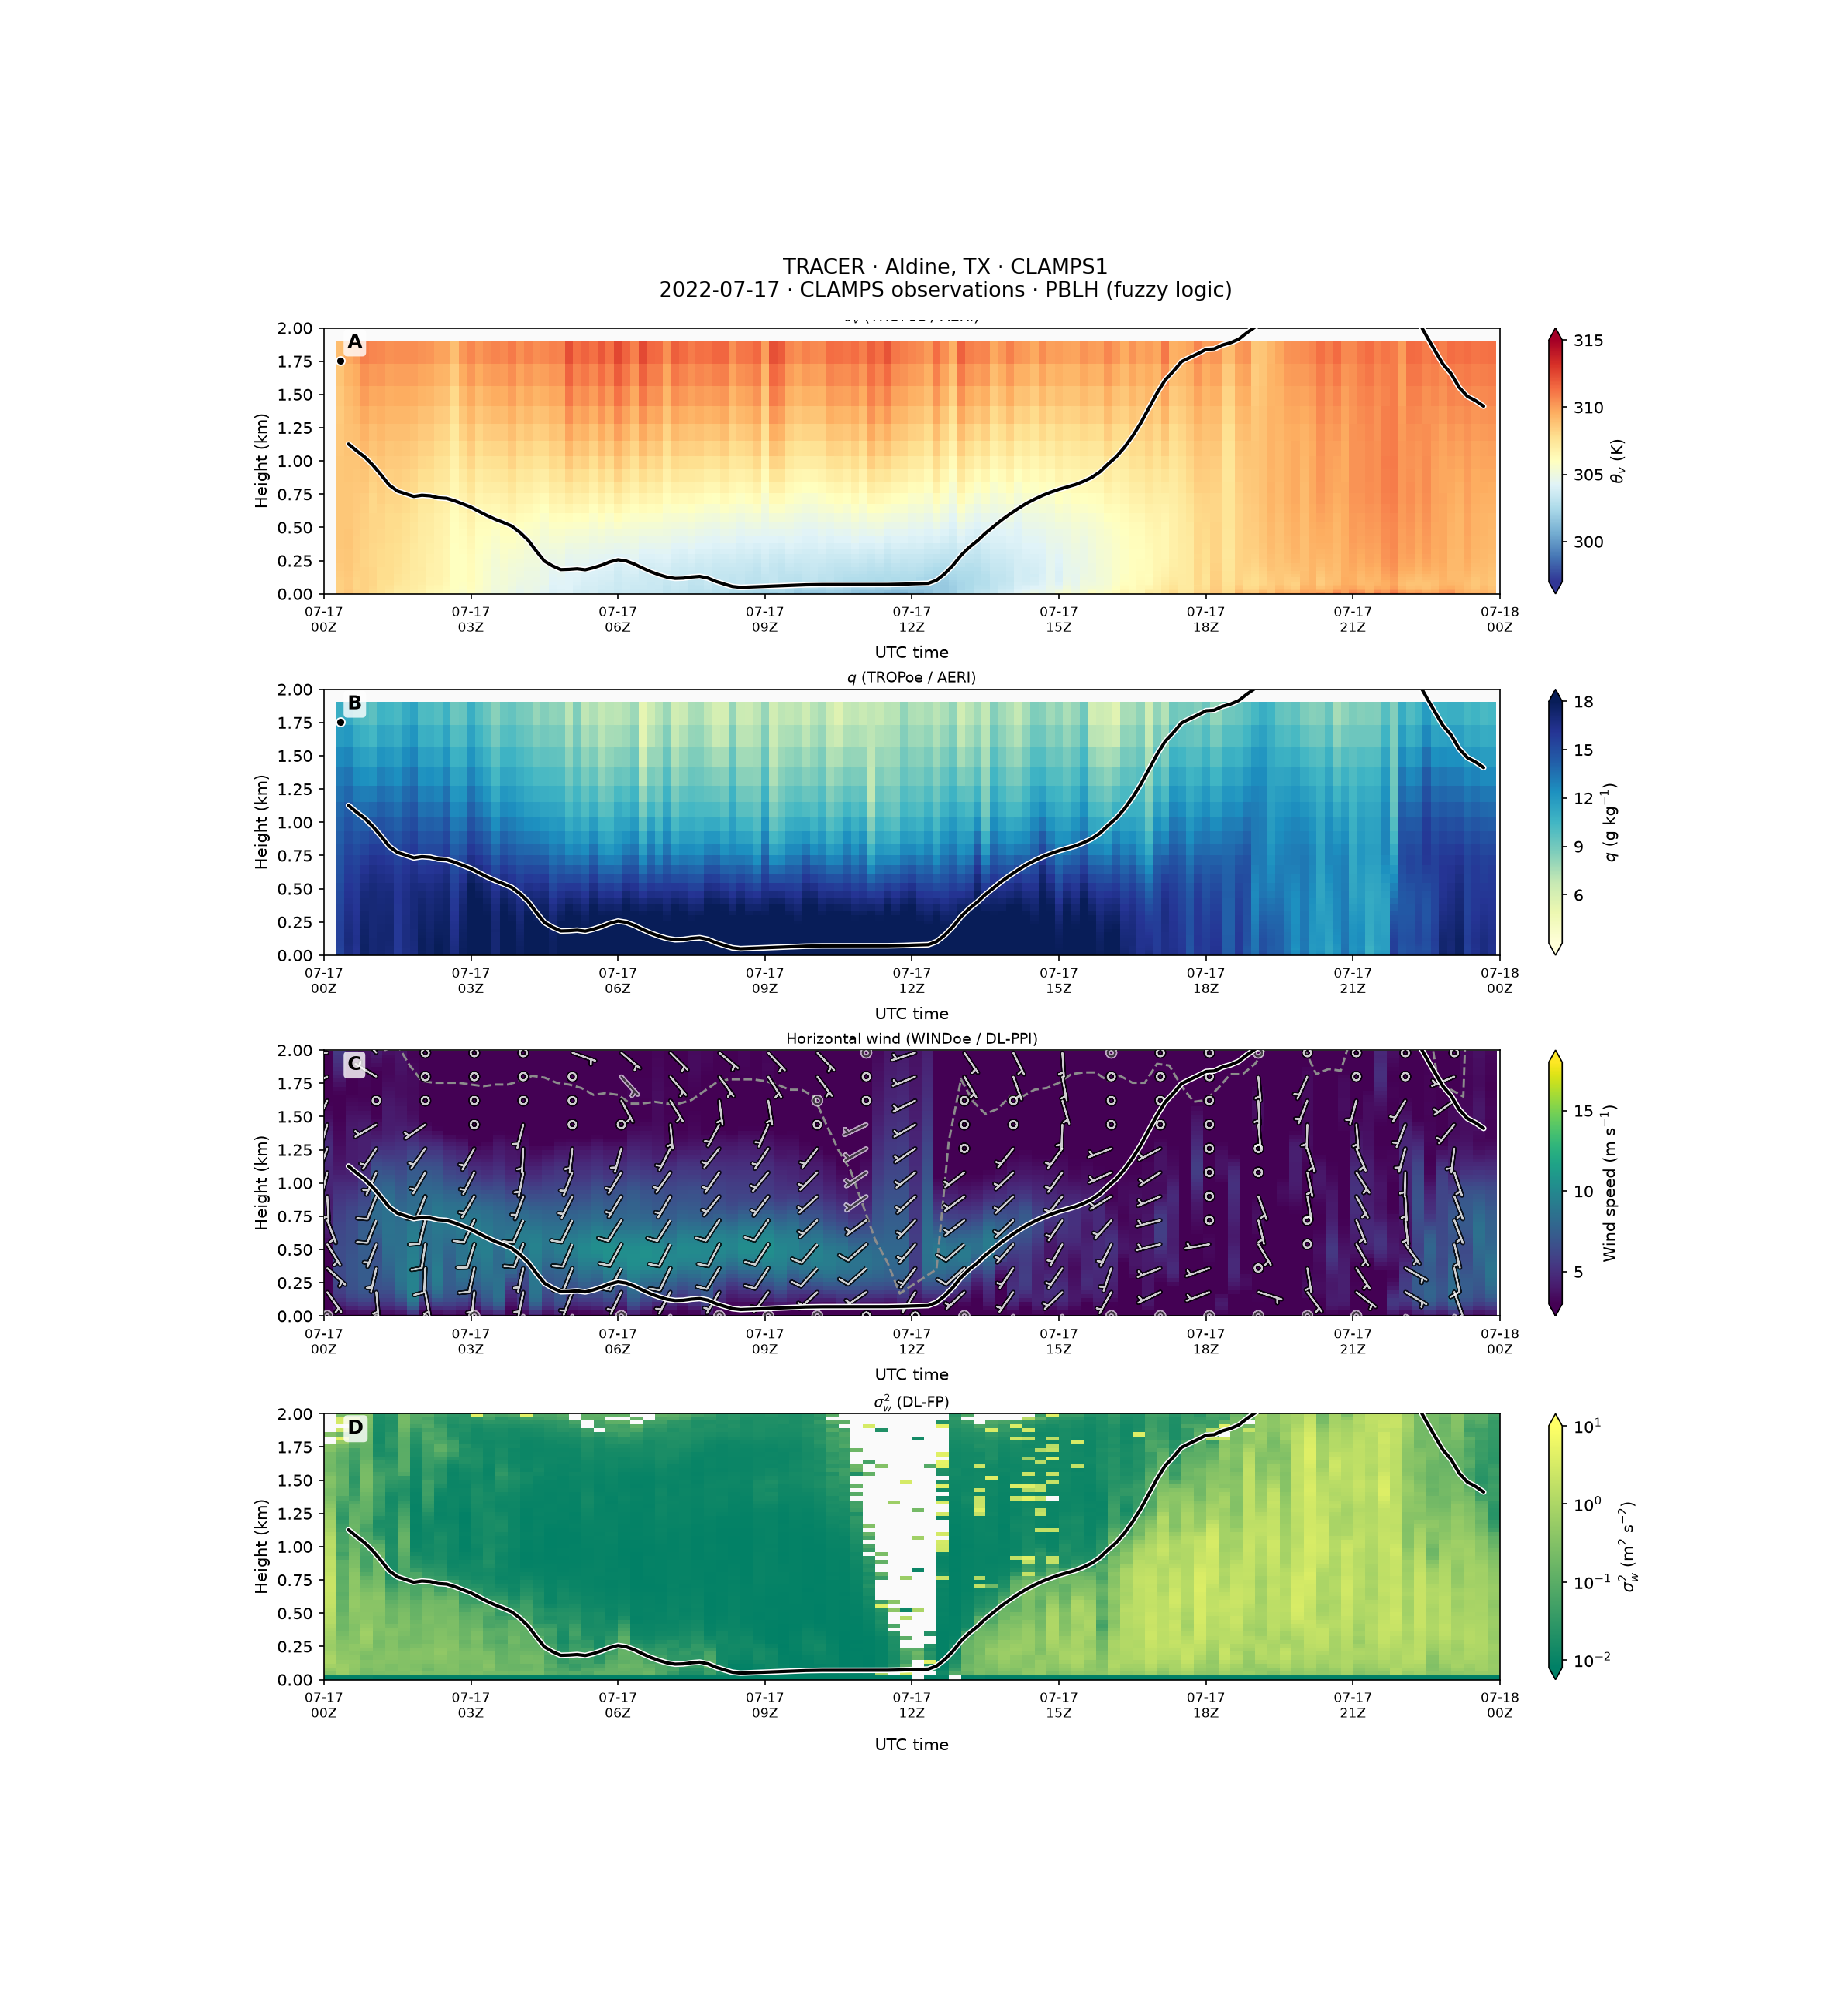
\includegraphics[width=\textwidth]{../../images/sea_breeze_c1_instrument_template_4panel.png}
  \caption{CLAMPS1 — Aldine, TX (inland).}
  \label{fig:sea_breeze:sea_breeze_c1_instrument_template_4panel}
\end{figure}
\begin{figure}[htbp]
  \centering
  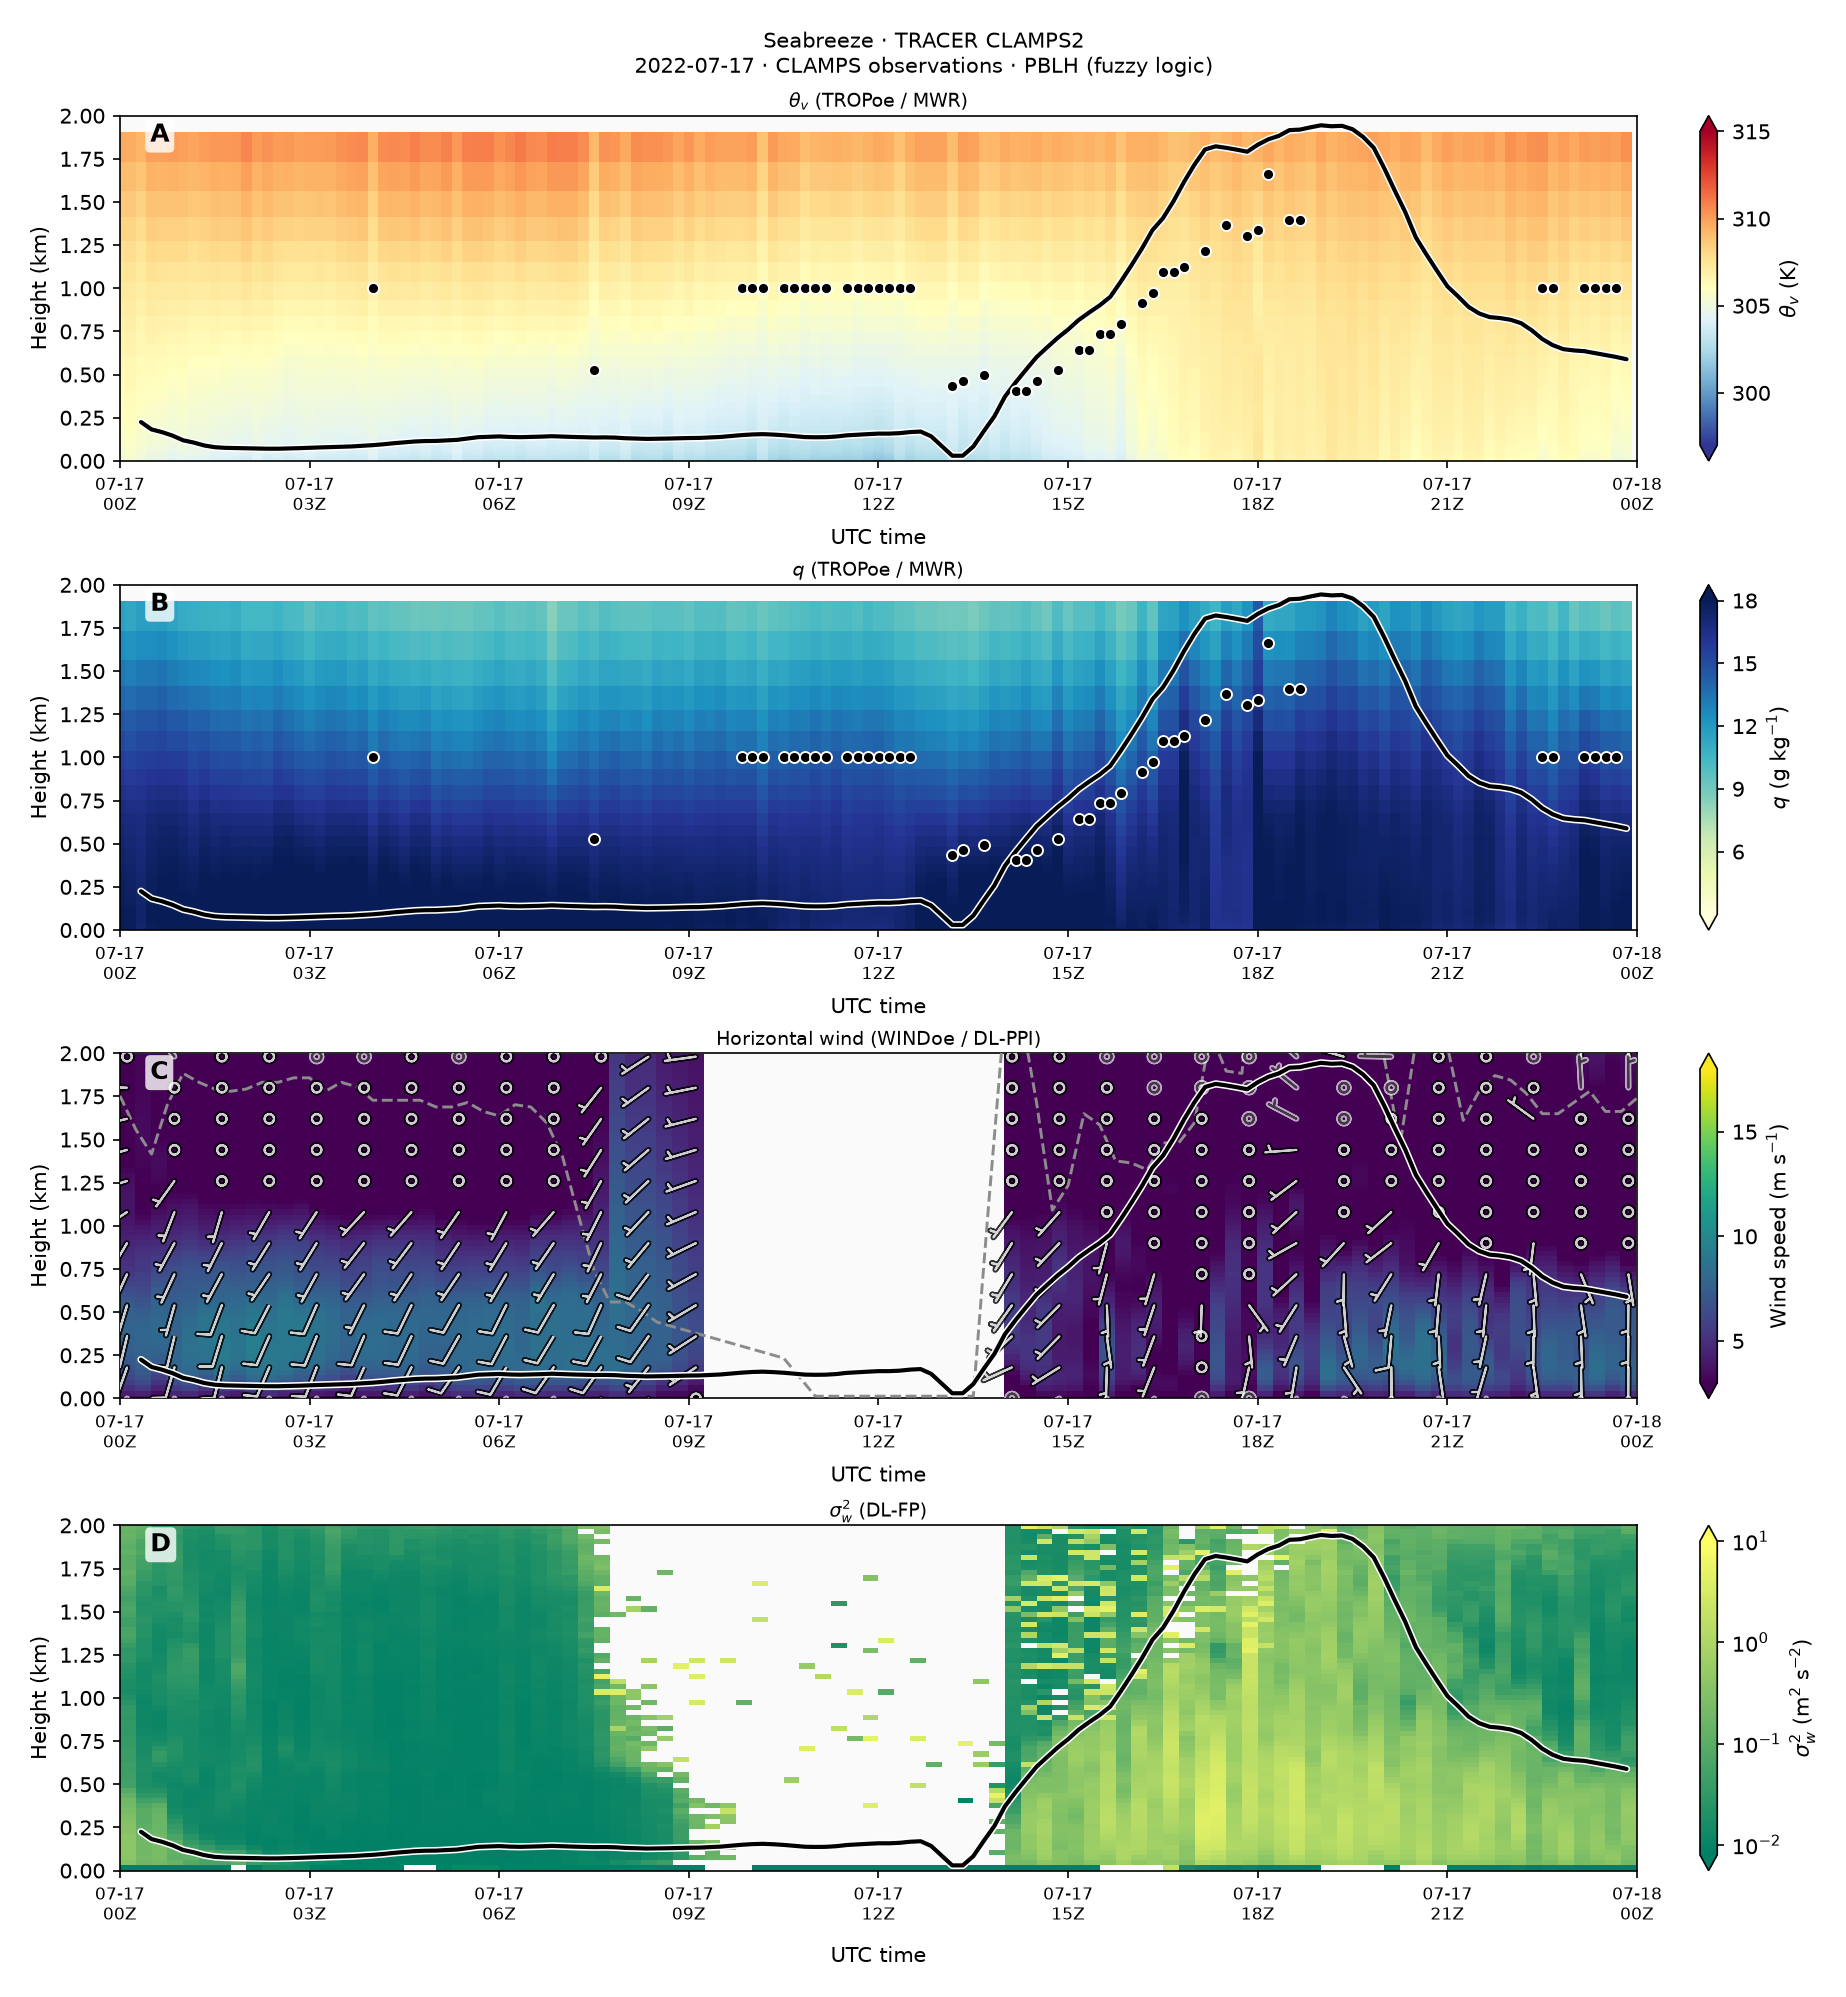
\includegraphics[width=\textwidth]{../../images/sea_breeze_c2_instrument_template_4panel.png}
  \caption{CLAMPS2 — La Marque, TX (coastal).}
  \label{fig:sea_breeze:sea_breeze_c2_instrument_template_4panel}
\end{figure}
\subsection*{Case overview}
This case highlights the simultaneous observation of a classic Gulf Coast sea breeze event by two co-deployed CLAMPS platforms during the TRACER campaign in the greater Houston, Texas area. CLAMPS2 was positioned near the coast (south of Houston toward Galveston), while CLAMPS1 was deployed further inland (north of Houston in Aldine). Together, these datasets capture the landward progression of rich marine air and the deep convective boundary layer (CBL) growth. Crucially, this case documents a common tropical coastal testing limitation: severe overnight lidar signal dropouts caused by dew condensing onto the lidar lens scanner window as high-moisture air cools to its dewpoint.

\subsection*{Highlights}
\begin{itemize}
  \item Thermal Environment \& Spatial Context (Panels A): As seen in the regional satellite view of \hyperref[fig:sea_breeze:sea_breeze_goes16_houston_seabreeze]{GOES-16 Houston area (17–24 UTC)}, CLAMPS2 is deployed near the immediate coastline while CLAMPS1 sits well inland. Consequently, CLAMPS2 exhibits a significantly tempered thermal profile overnight and early in the day due to marine proximity in panel A of \hyperref[fig:sea_breeze:sea_breeze_c2_instrument_template_4panel]{CLAMPS2 — La Marque, TX (coastal)}. In contrast, CLAMPS1 displays a more pronounced diurnal temperature swing in panel A of \hyperref[fig:sea_breeze:sea_breeze_c1_instrument_template_4panel]{CLAMPS1 — Aldine, TX (inland)}, with warmer afternoon virtual potential temperatures ($\theta_v \approx 312\text{ K}$) and a deeper convective boundary layer reaching nearly 2.0 km by 18:00 UTC.
  \item Moisture Profiles (Panels B): Both sites exhibit a remarkably wet boundary layer, but the marine source is distinct at the coast. Panel B of \hyperref[fig:sea_breeze:sea_breeze_c2_instrument_template_4panel]{CLAMPS2 — La Marque, TX (coastal)} shows that CLAMPS2 sustains an ultra-rich moisture column ($q \approx 15\text{ to }18\text{ g kg}^{-1}$) extending up to 1.5 km during the overnight hours. At CLAMPS1, panel B of \hyperref[fig:sea_breeze:sea_breeze_c1_instrument_template_4panel]{CLAMPS1 — Aldine, TX (inland)} captures a more suppressed and shallower moisture layer ($<1.0\text{ km}$) before daytime convective mixing distributes it upward.
  \item Lidar Lens Condensation Analysis (Panels C \& D): The most striking feature of this multi-station comparison is the timing and duration of the data dropouts (white gapping in $\sigma_w^2$ and blank/purple blocks in the wind profiles) across both \hyperref[fig:sea_breeze:sea_breeze_c1_instrument_template_4panel]{CLAMPS1 — Aldine, TX (inland)} and \hyperref[fig:sea_breeze:sea_breeze_c2_instrument_template_4panel]{CLAMPS2 — La Marque, TX (coastal)}. This instrumental limitation is explicitly quantified by overlaying surface relative humidity against lowest-gate lidar signal strength in \hyperref[fig:sea_breeze:sea_breeze_aux_seabreeze_rh_snr]{Surface RH \& DL-FP SNR (04–15 UTC)}.
  \item CLAMPS2 Coastal Dropout Window: Situated close to the Gulf moisture source, the coastal air mass reaches near-saturation rapidly. As detailed by the blue curves in \hyperref[fig:sea_breeze:sea_breeze_aux_seabreeze_rh_snr]{Surface RH \& DL-FP SNR (04–15 UTC)}, when surface RH climbs past 85\% at 07:30 UTC, the lowest-gate DL-FP SNR instantly collapses below $-25\text{ dB}$. This triggers a massive, prolonged lens condensation event lasting nearly 6.5 hours (from \textasciitilde{}07:30 UTC to 14:00 UTC in panel D of \hyperref[fig:sea_breeze:sea_breeze_c2_instrument_template_4panel]{CLAMPS2 — La Marque, TX (coastal)}), completely attenuating the lidar beam until solar heating evaporates the dew off the window.
  \item CLAMPS1 Inland Dropout Window: Farther inland at Aldine, lower ambient relative humidity delays saturation. As shown by the red curves in \hyperref[fig:sea_breeze:sea_breeze_aux_seabreeze_rh_snr]{Surface RH \& DL-FP SNR (04–15 UTC)}, the surface RH does not max out until \textasciitilde{}11:00 UTC, leading to a heavily mitigated lens condensation window that lasts only about 2 hours (from \textasciitilde{}10:30 UTC to 12:30 UTC in panel D of \hyperref[fig:sea_breeze:sea_breeze_c1_instrument_template_4panel]{CLAMPS1 — Aldine, TX (inland)}) before a rapid post-sunrise recovery occurs.
  \item Sea Breeze Frontal Arrival Timing: The inland progression of the sea breeze density current is beautifully mapped by the multi-parameter surface time series in \hyperref[fig:sea_breeze:sea_breeze_aux_seabreeze_arrival_meteogram]{Sea breeze arrival timing (17–22:30 UTC)}. The marine front impacts the coastal CLAMPS2 site first around 17:50 UTC (blue shaded column), marked by an immediate temperature drop, a sharp dewpoint surge up to $23^\circ\text{C}$, a wind shift to steady southerlies, and a sudden jump in surface RH. This exact cold-frontal signature is tracked marching inland, striking the CLAMPS1 site nearly four hours later at 21:35 UTC (red shaded column) with a dramatic $4^\circ\text{C}$ dewpoint surge and wind vector alignment.
  \item The Complementary Benefit: While the Doppler Lidars are blinded by dew during the overnight hours, the passive AERI and MWR thermodynamic retrieval profiles (Panels A and B of \hyperref[fig:sea_breeze:sea_breeze_c1_instrument_template_4panel]{CLAMPS1 — Aldine, TX (inland)} and \hyperref[fig:sea_breeze:sea_breeze_c2_instrument_template_4panel]{CLAMPS2 — La Marque, TX (coastal)}) remain entirely unbothered, demonstrating the massive operational resilience of a multi-instrument remote sensing suite in saturated environments.
\end{itemize}
\begin{figure}[htbp]
  \centering
  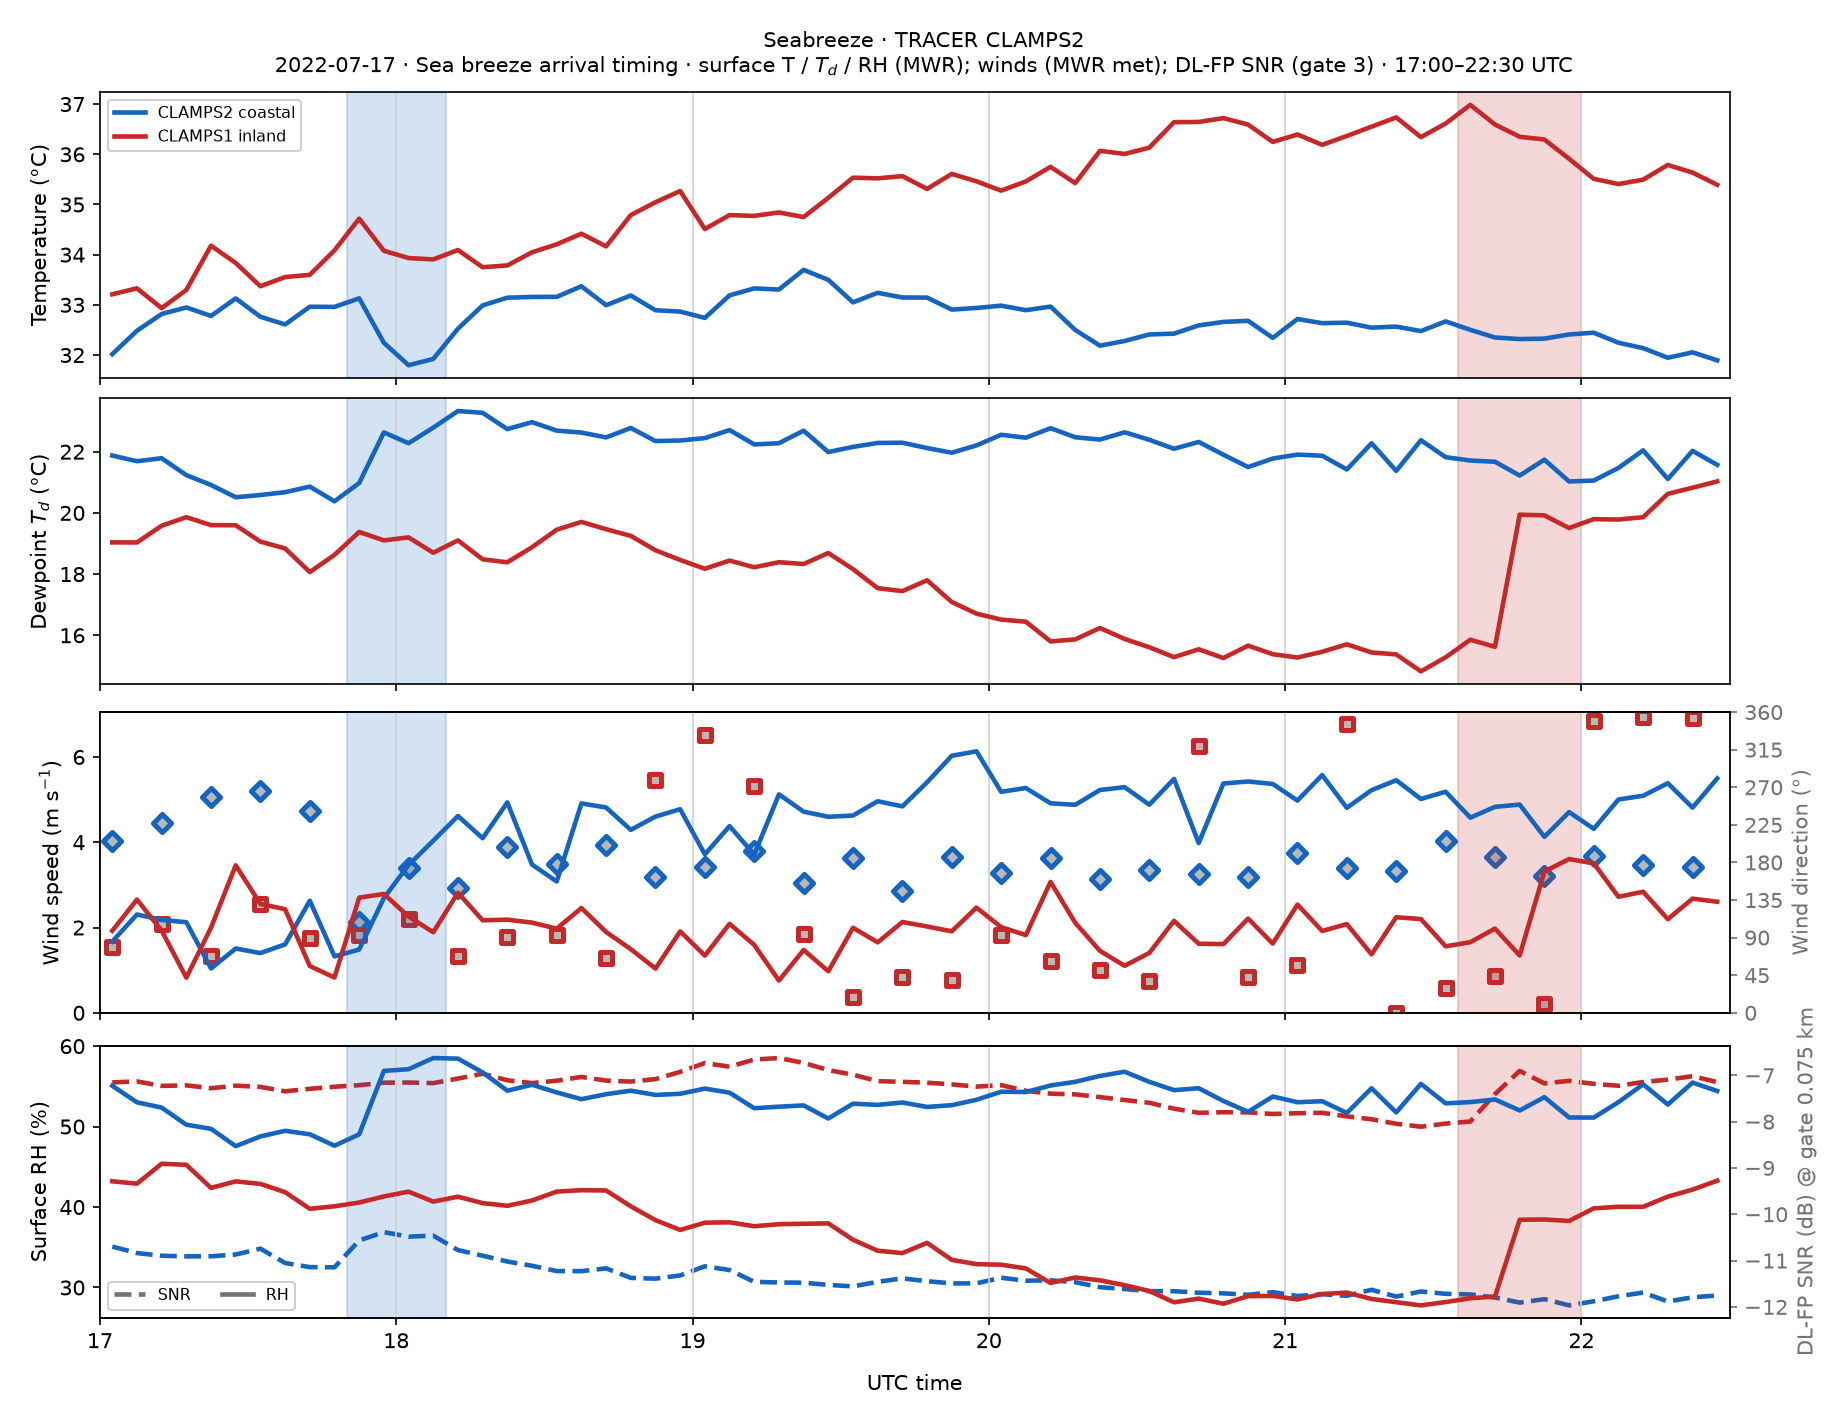
\includegraphics[width=0.92\textwidth]{../../images/sea_breeze_aux_seabreeze_arrival_meteogram.png}
  \caption{Sea breeze arrival timing (17–22:30 UTC).
  Multi-station surface comparison mapping sea-breeze frontal arrival at coastal CLAMPS2 ($\sim$17:50 UTC) and inland CLAMPS1 ($\sim$21:35 UTC) via temperature, dewpoint, wind, and RH signatures.}
  \label{fig:sea_breeze:sea_breeze_aux_seabreeze_arrival_meteogram}
\end{figure}
\begin{figure}[htbp]
  \centering
  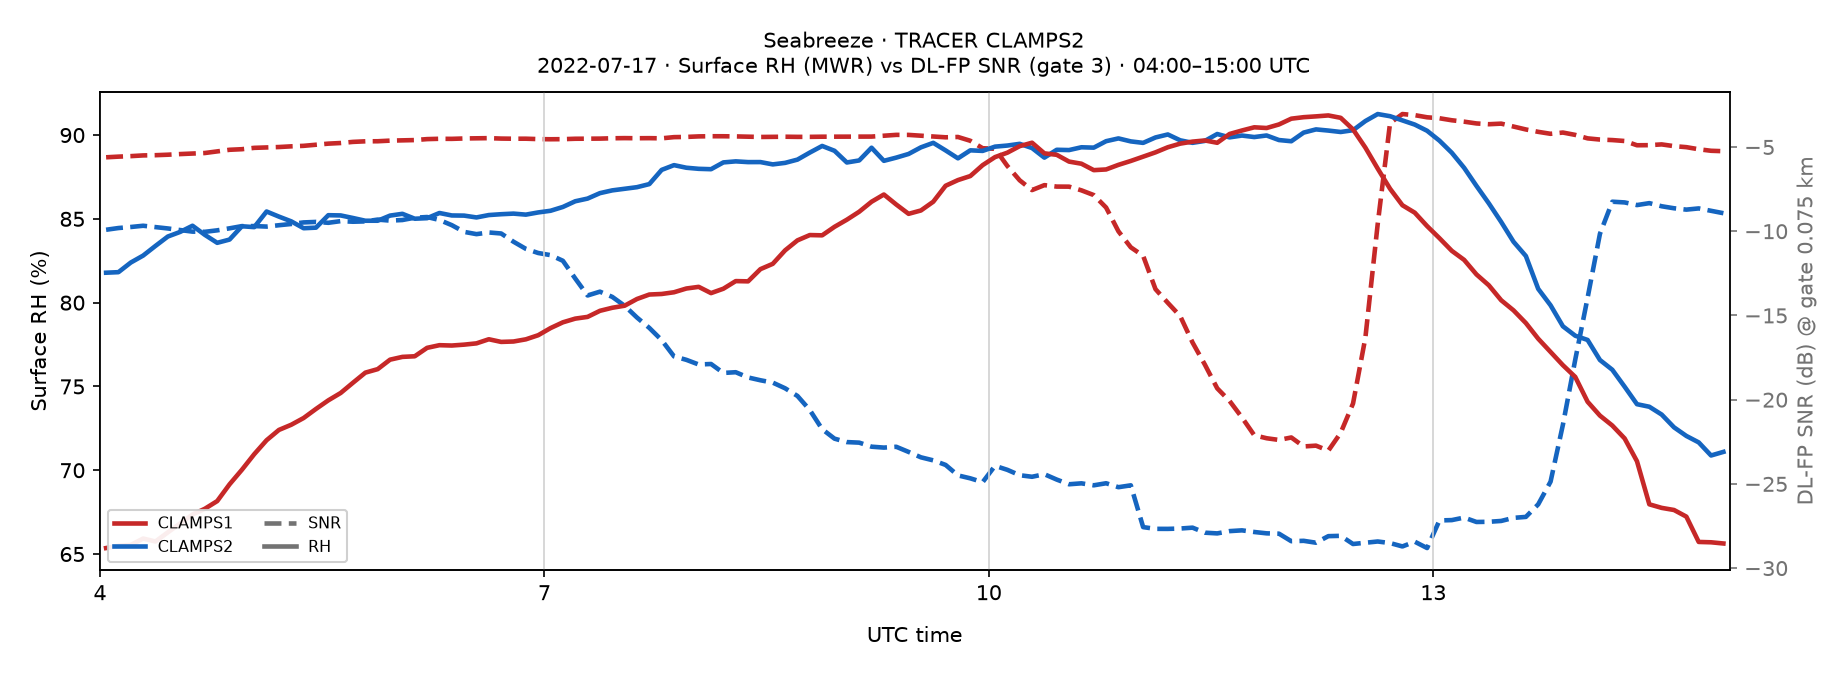
\includegraphics[width=0.92\textwidth]{../../images/sea_breeze_aux_seabreeze_rh_snr.png}
  \caption{Surface RH \& DL-FP SNR (04–15 UTC).
  Surface relative humidity overlaid on lowest-gate DL-FP SNR for CLAMPS2 (coastal) and CLAMPS1 (inland), quantifying lens-condensation dropout windows driven by overnight saturation.}
  \label{fig:sea_breeze:sea_breeze_aux_seabreeze_rh_snr}
\end{figure}
\begin{figure}[htbp]
  \centering
  \includegraphics[width=0.92\textwidth]{_frames/sea_breeze_goes16_houston_seabreeze.png}
  \caption{GOES-16 Houston area (17–24 UTC).
  GOES-16 visible imagery (17–24 UTC) showing the sea-breeze front advancing inland across the greater Houston area. First frame of animated loop; full animation available in the online gallery.}
  \label{fig:sea_breeze:sea_breeze_goes16_houston_seabreeze}
\end{figure}
\section{Deep Convective Boundary Layer}
\textit{CLAMPS1 $\cdot$ TRACER $\cdot$ Aldine, TX $\cdot$ July 20, 2022 $\cdot$ boundary layer, retrieval quality, CBL, coastal, limitations}

\begin{figure}[htbp]
  \centering
  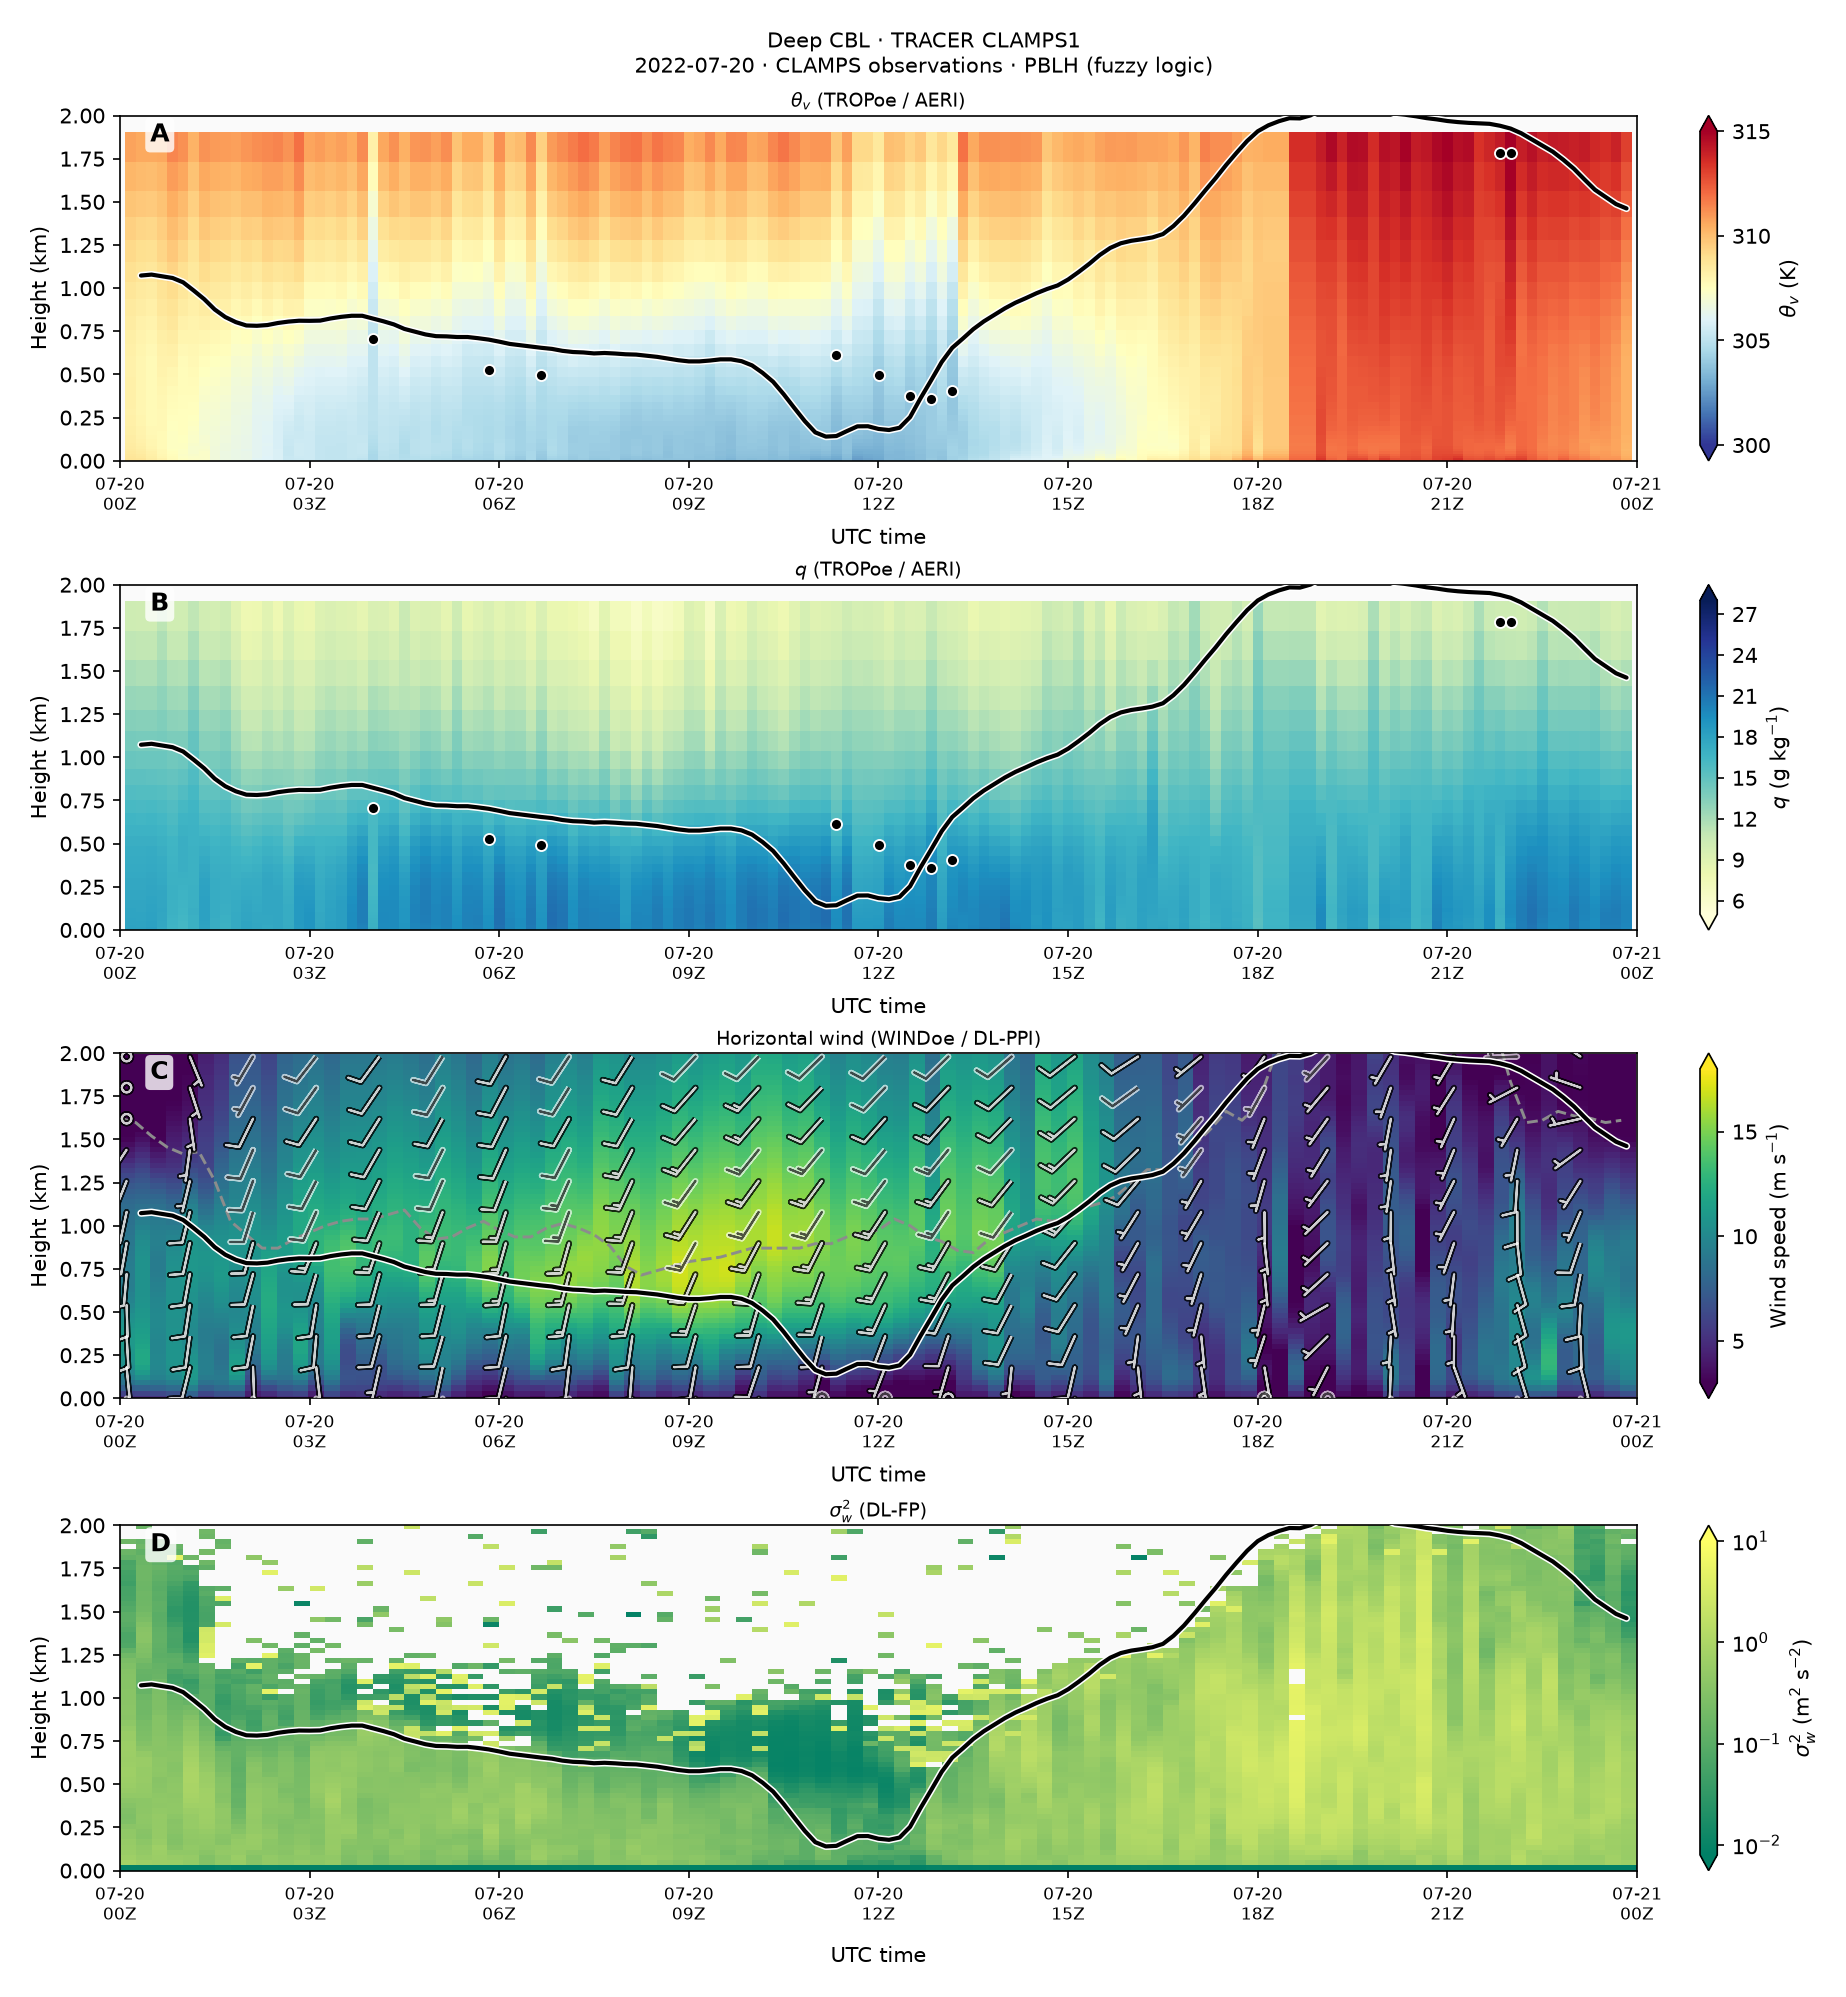
\includegraphics[width=\textwidth]{../../images/deep_cbl_c1_instrument_template_4panel.png}
  \caption{Standard CLAMPS observations.}
  \label{fig:deep_cbl_c1:deep_cbl_c1_instrument_template_4panel}
\end{figure}
\subsection*{Case overview}
This case showcases rapid growth of a deep, well-mixed convective boundary layer (CBL) over the Houston area during TRACER, but it is also an important cautionary example of thermodynamic retrieval behavior in an extremely moist Gulf Coast environment. Houston’s boundary layer often carries so much water vapor that continuum absorption contributes non-trivial radiance in the infrared window band. The legacy LBLRTM forward model used in TROPoe at the time could not faithfully reproduce that continuum signal. The optimal-estimation solver still tries to minimize observation–model misfit, and in this regime it can respond with unphysical adjustments—most commonly injecting excess moisture aloft and lowering temperature—to force a better radiance fit. The companion 18 and 19 UTC profile figure is included specifically to illustrate this issue: retrieval quality metrics and profile shape are much worse around 18 UTC, then improve by 19 UTC as daytime mixing modestly reduces low-level moisture and stabilizes the solution.

\subsection*{Highlights}
\begin{itemize}
  \item Thermodynamic retrieval instability (Panels A \& B; 18 UTC): In the early afternoon, when boundary-layer moisture is especially extreme, TROPoe can produce suspicious upper-level moistening and cooling that are not supported by the broader thermodynamic context in \hyperref[fig:deep_cbl_c1:deep_cbl_c1_instrument_template_4panel]{Standard CLAMPS observations}. The standalone profile cut in \hyperref[fig:deep_cbl_c1:deep_cbl_c1_aux_tropoe_t_q_profiles_18_19]{TROPoe $\theta_v$ and $q$ profiles at 18 and 19 UTC} quantifies this failure at 18:00 UTC (solid black lines); a large residual mean square absolute (RMSA = 8.97) and high residual mean square ratio (RMSR = 9.00) reveal that the forward model is mathematically struggling to match observed window-region radiances even after forcing these unphysical thermodynamic vertical structures.
  \item Improved stability after mixing (19 UTC profiles): By 19:00 UTC, the retrieval metrics in \hyperref[fig:deep_cbl_c1:deep_cbl_c1_aux_tropoe_t_q_profiles_18_19]{TROPoe $\theta_v$ and $q$ profiles at 18 and 19 UTC} stabilize drastically (dashed lines), with RMSA collapsing to 0.68 and RMSR dropping to 0.67. This indicates that continued daytime turbulent boundary layer mixing successfully scoured out the most extreme low-level stagnant moisture, reducing the infrared continuum-dominated misfit enough for the physical forward model solver to converge into a representative solution.
  \item Deep CBL growth despite retrieval challenges (Panel A): Even with early-period thermodynamic artifacts, \hyperref[fig:deep_cbl_c1:deep_cbl_c1_instrument_template_4panel]{Standard CLAMPS observations} still captures the macro-scale diurnal transition. Virtual potential temperature ($\theta_v$) shows strong afternoon warming and deep vertical uniformization. This progressive boundary layer growth is captured as a step-wise erosion of the morning capping inversion in \hyperref[fig:deep_cbl_c1:deep_cbl_c1_aux_mixed_layer_profiles]{Mixed-layer vertical profiles}, with the fuzzy-logic PBLH line tracking the mixed layer cleanly up to the 2.0 km display ceiling by 18:00 UTC.
  \item Moisture redistribution and surface background (Panel B): Specific humidity ($q$) reflects an ultra-moist coastal boundary layer. To properly contextualize these profiles, the 24-hour surface records in \hyperref[fig:deep_cbl_c1:deep_cbl_c1_aux_surface_meteogram]{Surface meteogram (full day)} and the high-resolution subset in \hyperref[fig:deep_cbl_c1:deep_cbl_c1_aux_surface_meteogram_17_20]{Surface meteogram (17–20 UTC)} show surface temperatures hovering near $36^\circ\text{C}$ with relative humidity values remaining remarkably high ($35\%\text{ to }40\%$) despite peak afternoon solar heating, confirming the intense local moisture reservoir that initiated the early-afternoon retrieval artifacts.
  \item Afternoon momentum and turbulence (Panels C \& D): Horizontal winds in panel C of \hyperref[fig:deep_cbl_c1:deep_cbl_c1_instrument_template_4panel]{Standard CLAMPS observations} become relatively uniform with height through the deep mixed layer during peak CBL growth, dropping below $5\text{ m s}^{-1}$ as convective mixing dominates. Concurrently, the vertical velocity variance ($\sigma_w^2$, panel D) increases sharply after the morning transition, providing clear statistical evidence of vigorous buoyant updrafts and downdrafts overturning the destabilized column.
\end{itemize}
\begin{figure}[htbp]
  \centering
  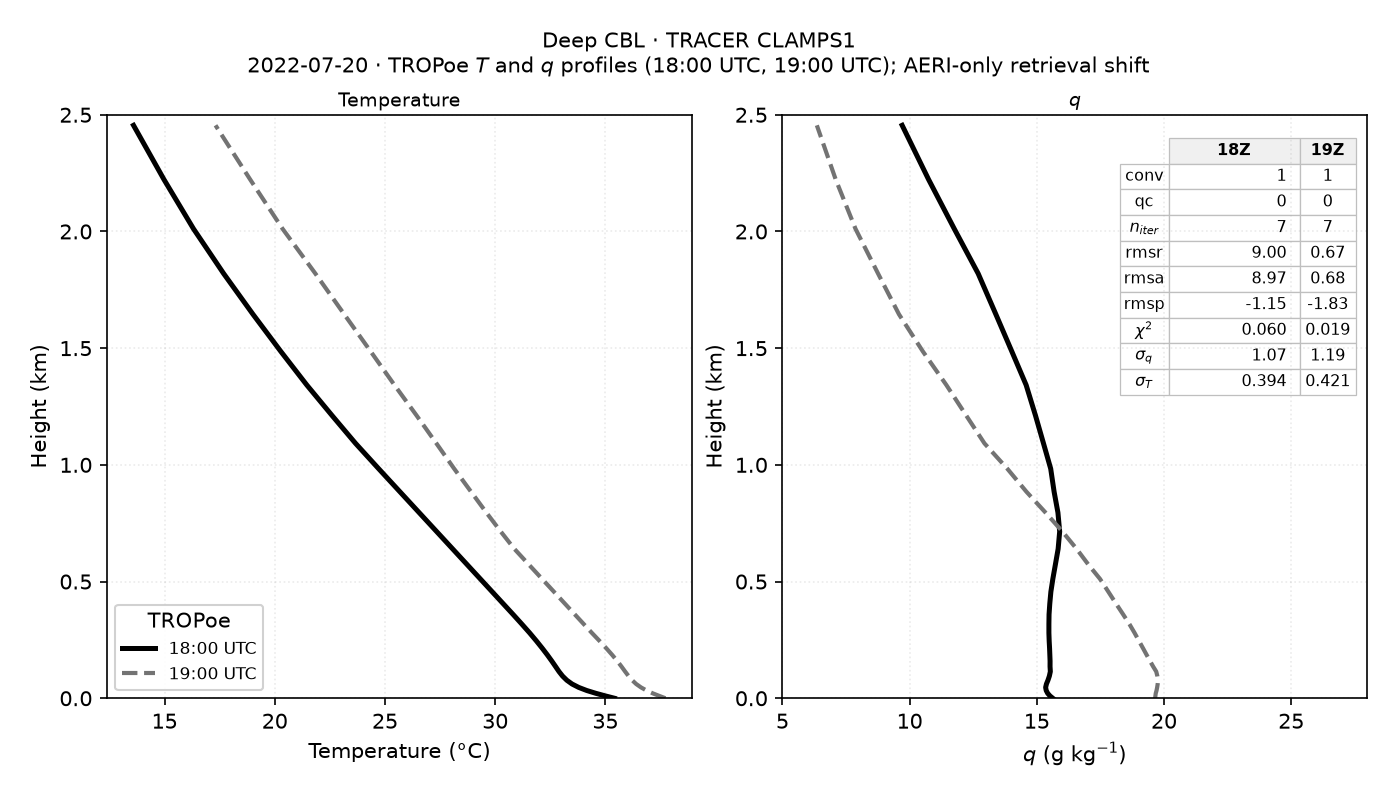
\includegraphics[width=0.92\textwidth]{../../images/deep_cbl_c1_aux_tropoe_t_q_profiles_18_19.png}
  \caption{TROPoe $\theta_v$ and $q$ profiles at 18 and 19 UTC.
  Standalone TROPoe $\theta_v$ and $q$ profiles at 18:00 and 19:00 UTC with retrieval quality metrics (RMSA, RMSR), illustrating early-afternoon infrared-continuum artifacts in the Houston marine environment.}
  \label{fig:deep_cbl_c1:deep_cbl_c1_aux_tropoe_t_q_profiles_18_19}
\end{figure}
\begin{figure}[htbp]
  \centering
  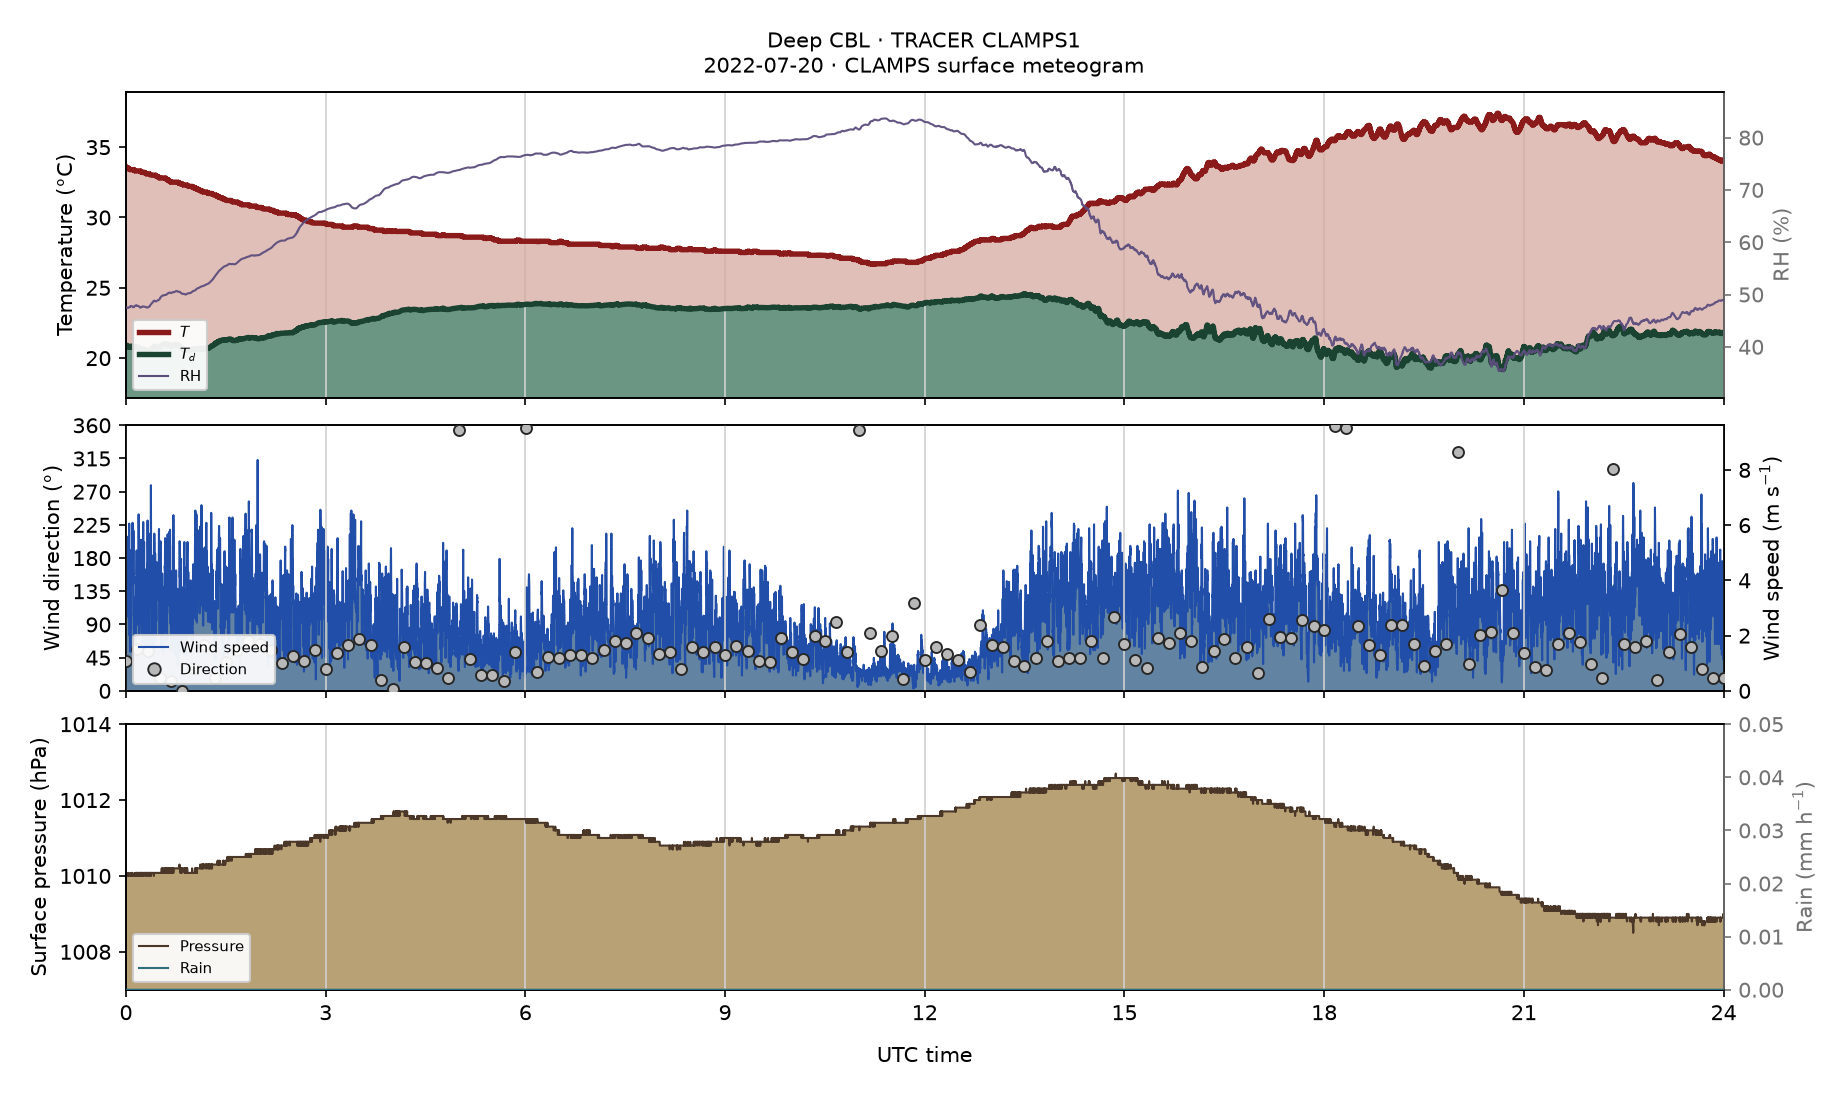
\includegraphics[width=0.92\textwidth]{../../images/deep_cbl_c1_aux_surface_meteogram.png}
  \caption{Surface meteogram (full day).
  24-hour surface temperature, humidity, and pressure providing regional context for the ultra-moist Gulf Coast boundary layer during TRACER.}
  \label{fig:deep_cbl_c1:deep_cbl_c1_aux_surface_meteogram}
\end{figure}
\begin{figure}[htbp]
  \centering
  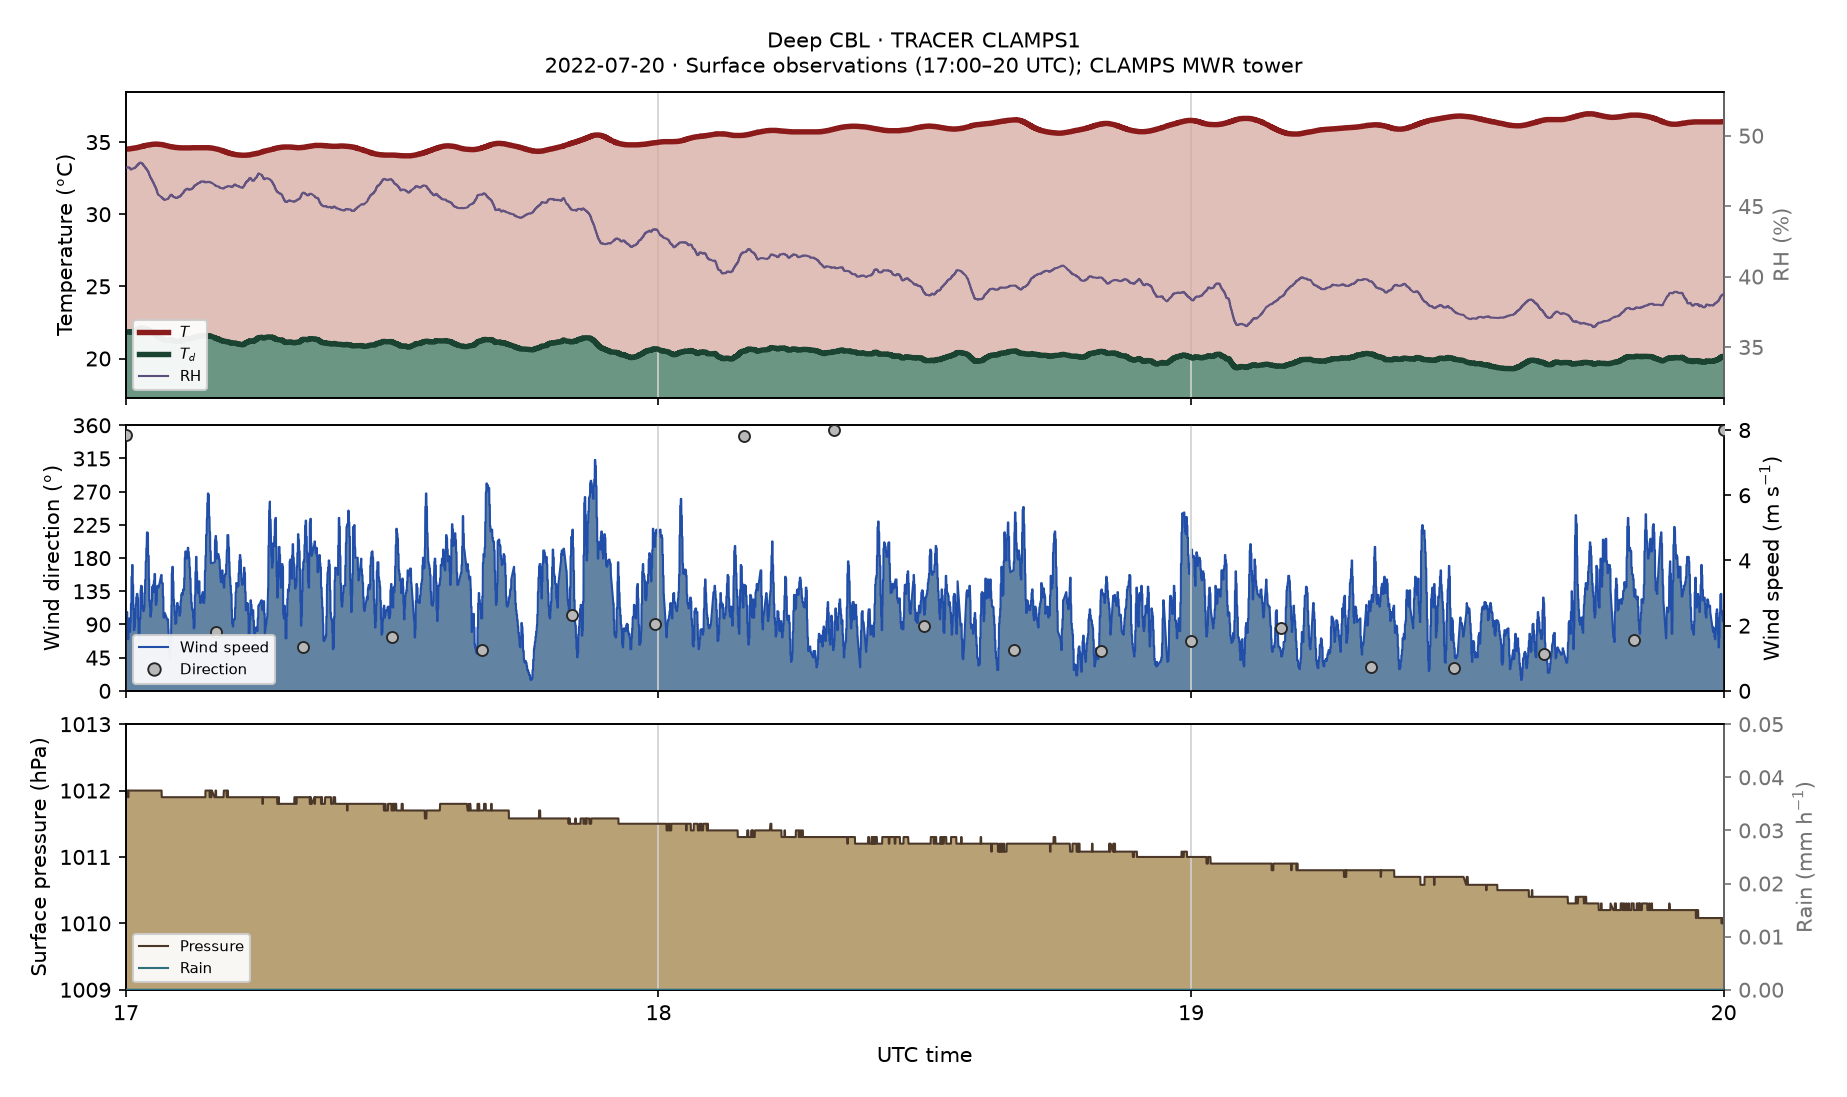
\includegraphics[width=0.92\textwidth]{../../images/deep_cbl_c1_aux_surface_meteogram_17_20.png}
  \caption{Surface meteogram (17–20 UTC).
  Afternoon surface meteogram subset showing peak temperatures near $36^\circ\mathrm{C}$ with persistently high relative humidity despite intense solar heating.}
  \label{fig:deep_cbl_c1:deep_cbl_c1_aux_surface_meteogram_17_20}
\end{figure}
\begin{figure}[htbp]
  \centering
  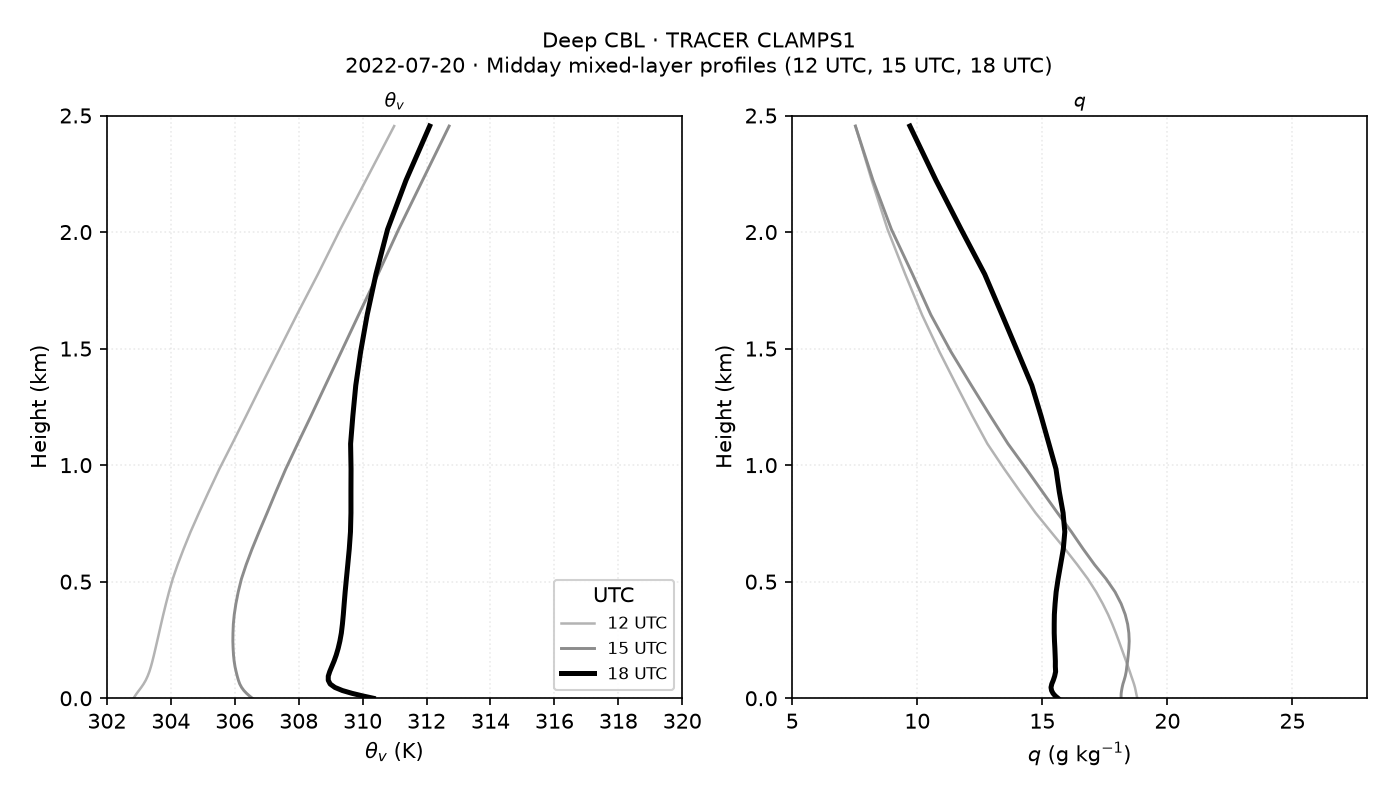
\includegraphics[width=0.92\textwidth]{../../images/deep_cbl_c1_aux_mixed_layer_profiles.png}
  \caption{Mixed-layer vertical profiles.
  Step-wise midday $\theta_v$ and $q$ profiles documenting progressive erosion of the morning capping inversion as the convective boundary layer deepens.}
  \label{fig:deep_cbl_c1:deep_cbl_c1_aux_mixed_layer_profiles}
\end{figure}
\section{Stable Boundary Layer — Good Lidar Quality}
\textit{CLAMPS2 $\cdot$ NWC Ops $\cdot$ Norman, OK $\cdot$ December 2, 2022 $\cdot$ stable, boundary layer, winter}

\begin{figure}[htbp]
  \centering
  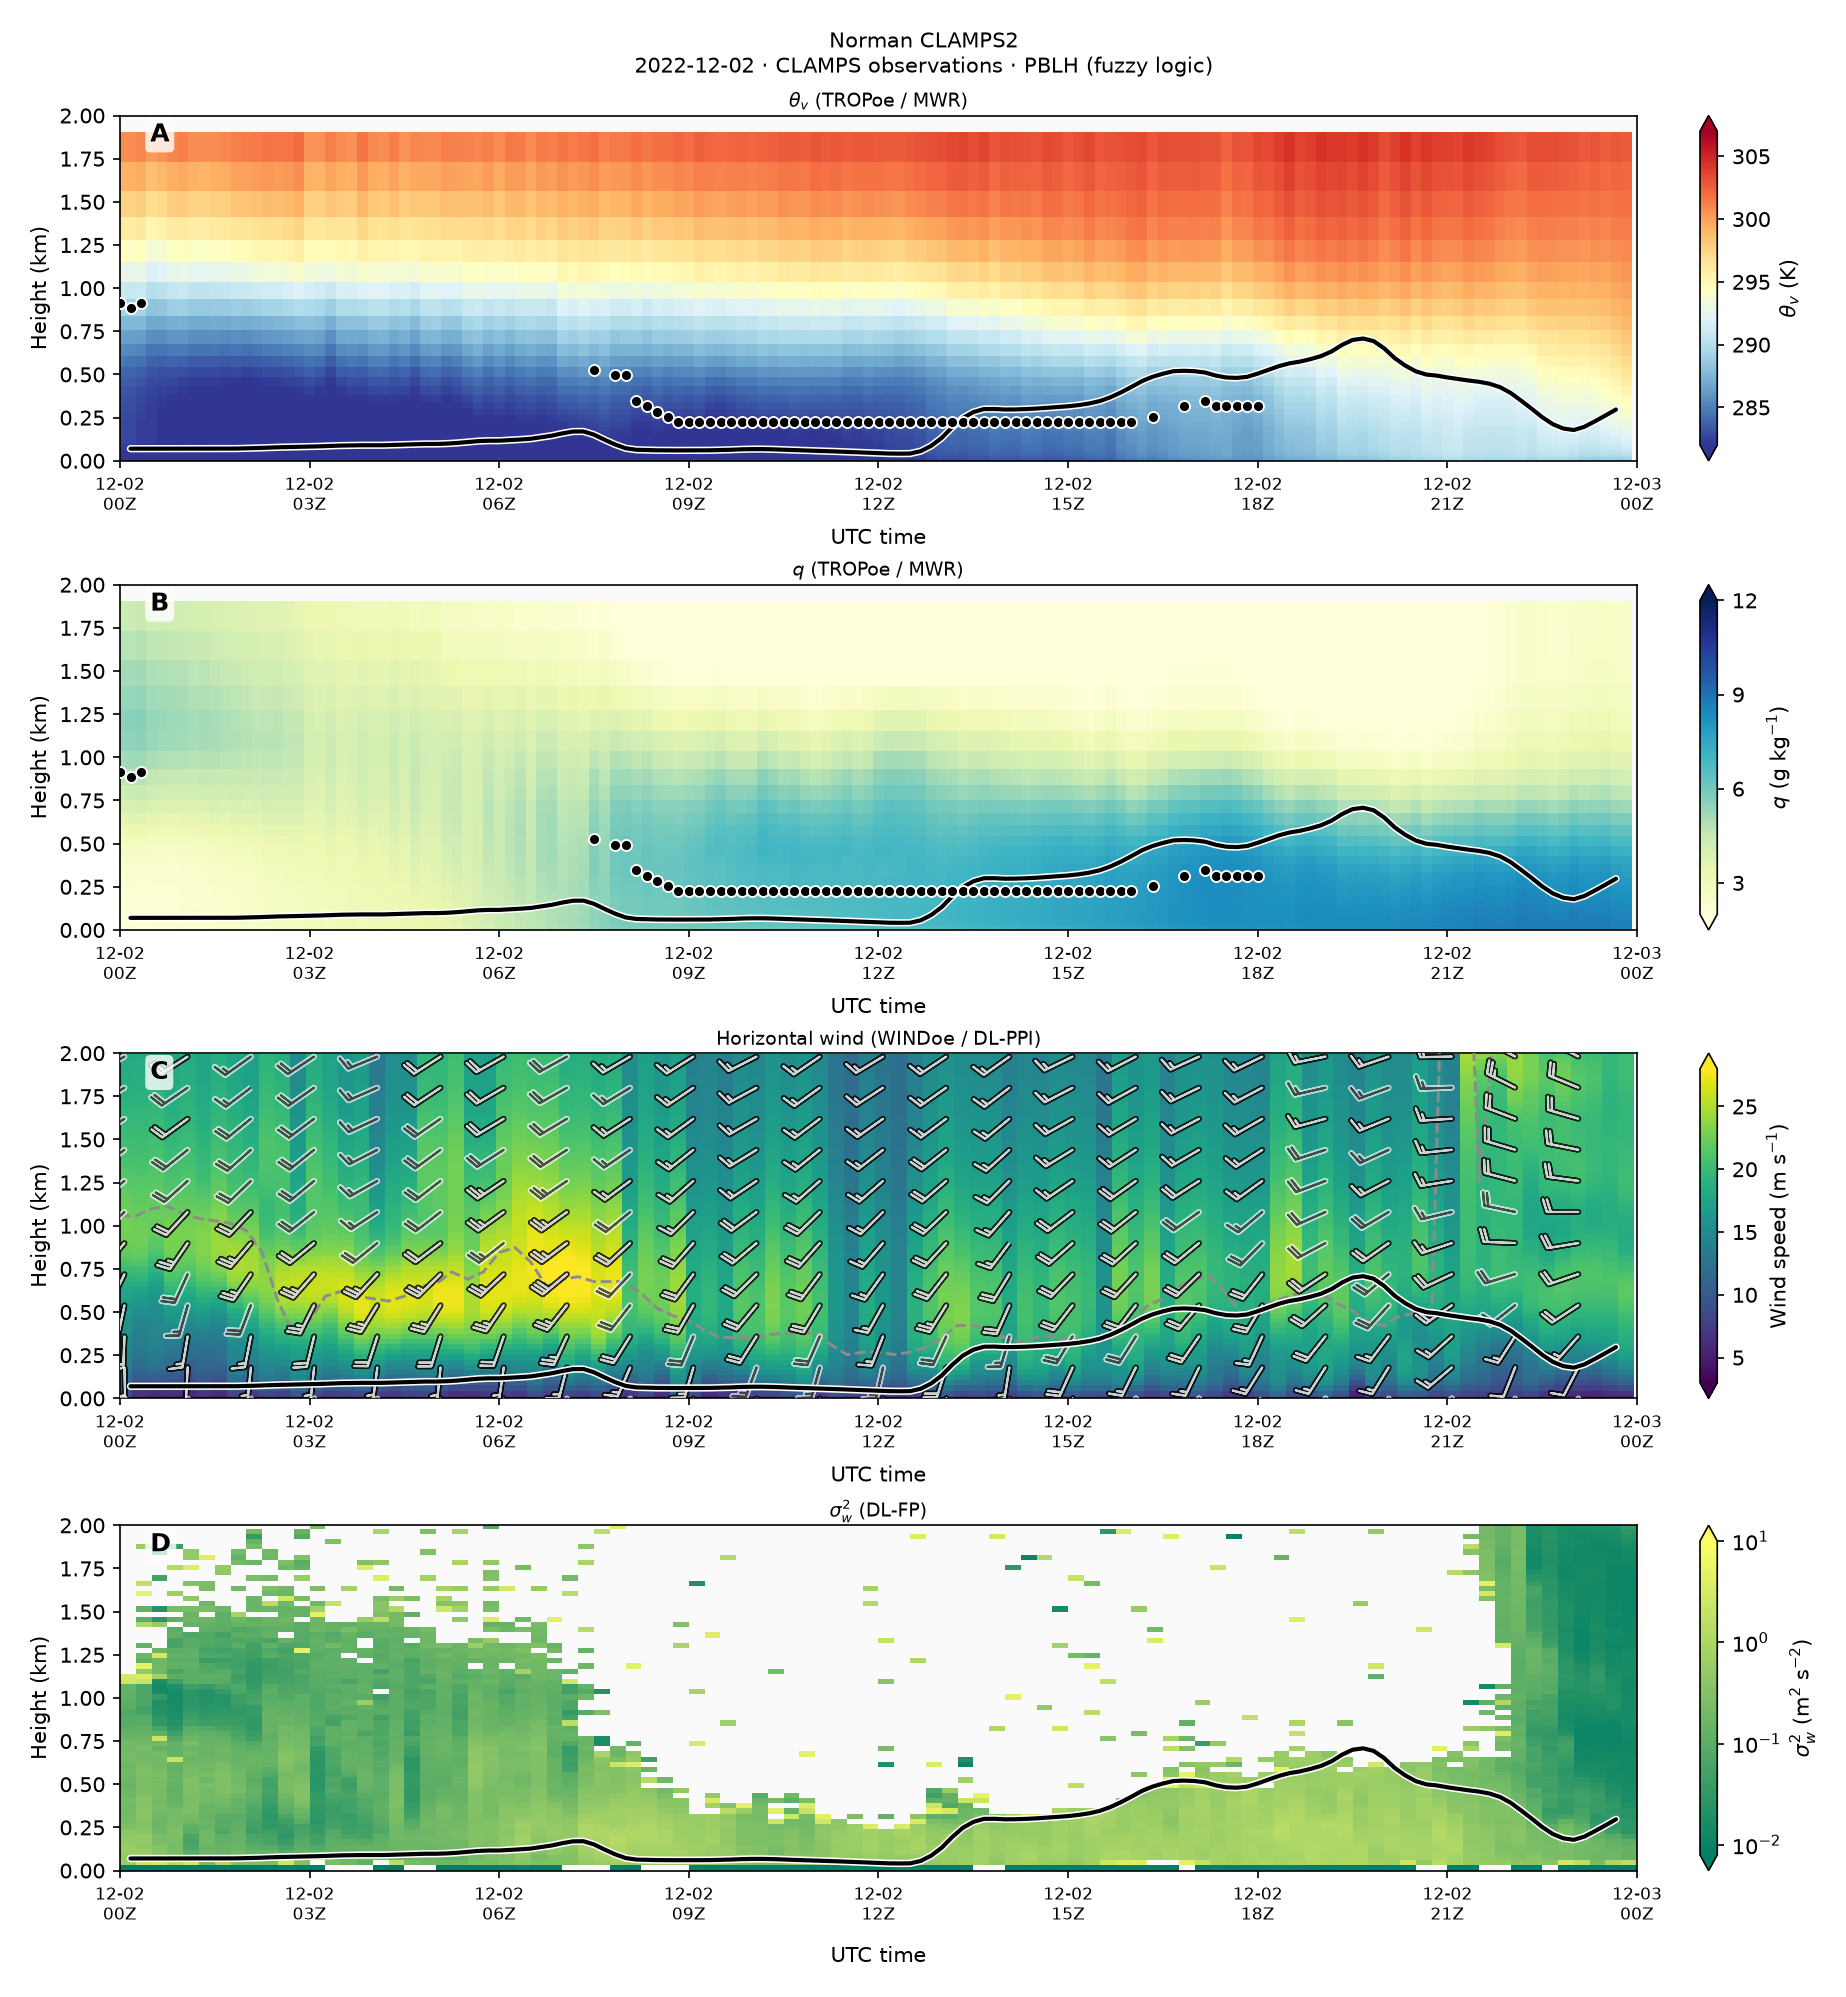
\includegraphics[width=\textwidth]{../../images/stable_good_dl_c2_instrument_template_4panel.png}
  \caption{Standard CLAMPS observations.}
  \label{fig:stable_good_dl_c2:stable_good_dl_c2_instrument_template_4panel}
\end{figure}
\subsection*{Case overview}
This winter case provides a textbook example of a strongly stratified stable boundary layer (SBL) under high-shear conditions. Unlike summer cases where intense solar insulation rapidly erodes nocturnal structures, the weak wintertime sun is unable to break the robust low-level thermal inversion, allowing stable stratification to dominate the entire diurnal cycle. Crucially, this case demonstrates good Doppler lidar data quality. The instrument successfully maintains a high signal-to-noise ratio throughout the deep column, beautifully capturing an intense, low-level synoptic wind maximum exceeding $25\text{ m s}^{-1}$ and the shear-driven turbulence it generates.

\subsection*{Highlights}
\begin{itemize}
  \item Persistent Thermal Inversion (Panel A): Near-surface virtual potential temperature ($\theta_v$) remains locked in a cold state ($< 285\text{ K}$, deep blue shading) throughout the first half of the period in \hyperref[fig:stable_good_dl_c2:stable_good_dl_c2_instrument_template_4panel]{Standard CLAMPS observations}. The fuzzy-logic boundary layer height (PBLH) line remains heavily suppressed below 250 m for the first 13 hours. Even during peak daylight hours (15:00 to 21:00 UTC), there is no true convective breakout; the inversion merely modifies slightly, rising to a shallow \textasciitilde{}500 m.
  \item Dry Continental Air Mass \& Synoptic Evolution (Panel B): Consistent with a cold post-frontal winter air mass, the specific humidity ($q$) in \hyperref[fig:stable_good_dl_c2:stable_good_dl_c2_instrument_template_4panel]{Standard CLAMPS observations} begins exceptionally low, flatlining between $3\text{ to }5\text{ g kg}^{-1}$ through the column. This background state matches the surface patterns tracked in \hyperref[fig:stable_good_dl_c2:stable_good_dl_c2_aux_surface_meteogram]{Surface meteogram}, which records sub-zero dewpoints ($T_d \approx -8^\circ\text{C}$) and a steadily falling meteogram pressure curve ($977.5\text{ to }967.5\text{ hPa}$), marking a strong synoptic-scale draw that drives warm, moist advection into the region later in the day.
  \item High-Velocity Wind Maximum (Panel C): In stark contrast to aerosol-depleted failure cases, the horizontal wind field in \hyperref[fig:stable_good_dl_c2:stable_good_dl_c2_instrument_template_4panel]{Standard CLAMPS observations} is exceptionally clean and complete. A powerful low-level wind maximum is observed between 00:00 UTC and 08:00 UTC, with wind speeds peaking above $25\text{ m s}^{-1}$ (bright yellow core) between 500 m and 1.0 km. The wind barbs capture strong westerly winds aloft shifting to north-westerly over time, a signature of the intense pressure gradient force mapped at the surface by the falling barometer.
  \item Shear-Driven Turbulence \& Stability Demarcation (Panel D): The vertical velocity variance ($\sigma_w^2$) beautifully maps the fluid dynamics of the column in \hyperref[fig:stable_good_dl_c2:stable_good_dl_c2_instrument_template_4panel]{Standard CLAMPS observations}. Between 00:00 and 07:00 UTC, the intense vertical wind shear underneath the jet core mechanically generates a deep layer of turbulence ($1\text{ to }2\text{ m}^2\text{ s}^{-2}$). This mechanical engine is directly corroborated by \hyperref[fig:stable_good_dl_c2:stable_good_dl_c2_aux_rib_timeheight]{Bulk Richardson number time–height}, where a large lower-tropospheric block plunges below the critical threshold ($Ri_b < 0.25$, red contours). Once the core wind speed diminishes and $Ri_b$ transitions to strongly stable conditions (blue shading aloft), the mechanical engine shuts off, and the column plunges into a quiet, non-turbulent laminar state.
\end{itemize}
\begin{figure}[htbp]
  \centering
  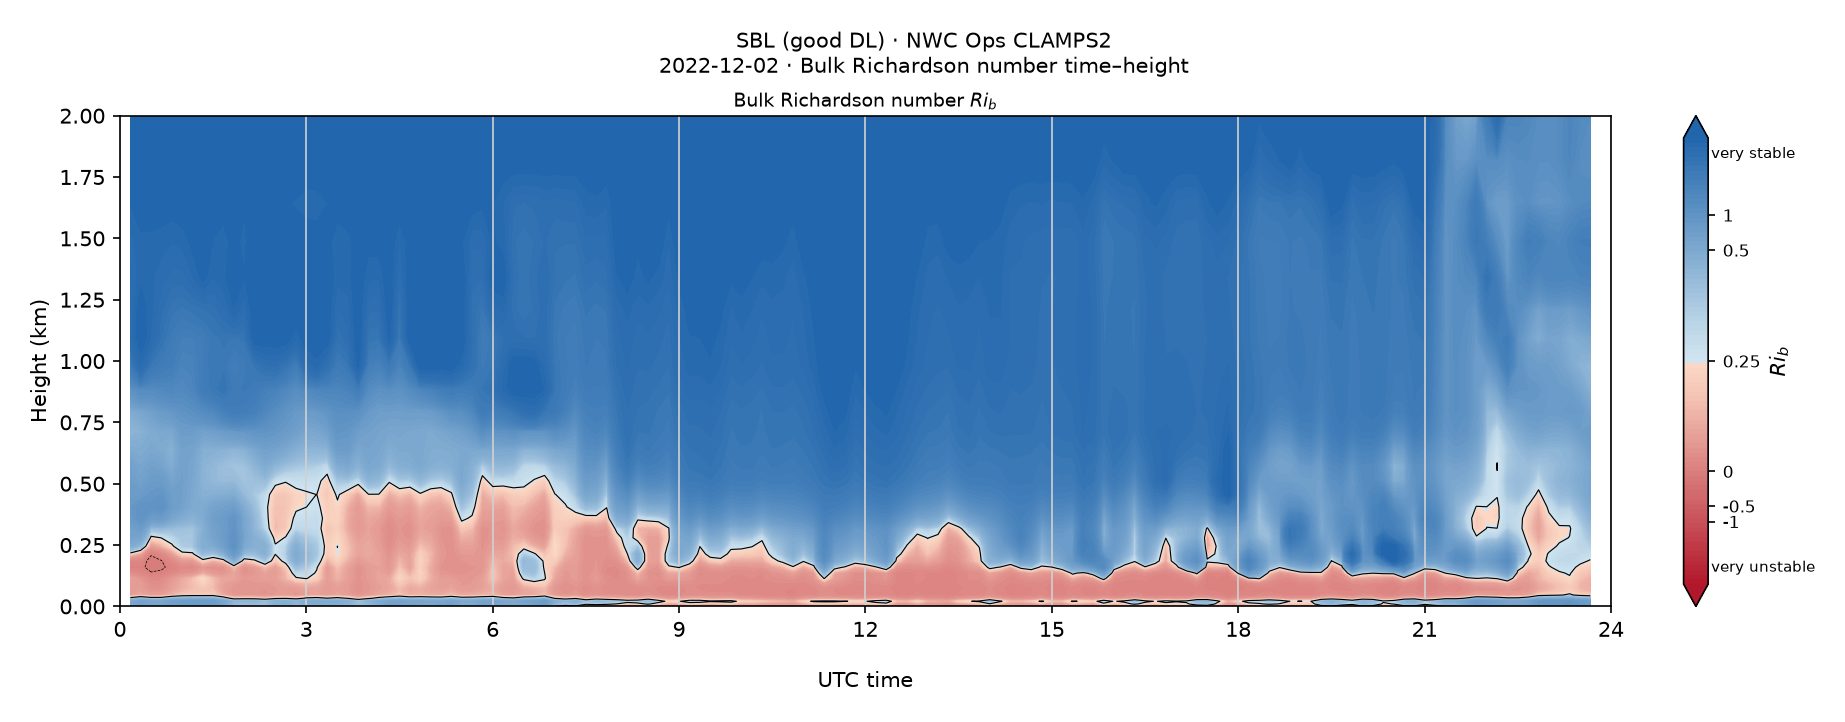
\includegraphics[width=0.92\textwidth]{../../images/stable_good_dl_c2_aux_rib_timeheight.png}
  \caption{Bulk Richardson number time–height.
  Bulk Richardson number $Ri_b$ mapping mechanically generated turbulence ($Ri_b < 0.25$) beneath the nocturnal low-level jet and the transition to laminar flow aloft.}
  \label{fig:stable_good_dl_c2:stable_good_dl_c2_aux_rib_timeheight}
\end{figure}
\begin{figure}[htbp]
  \centering
  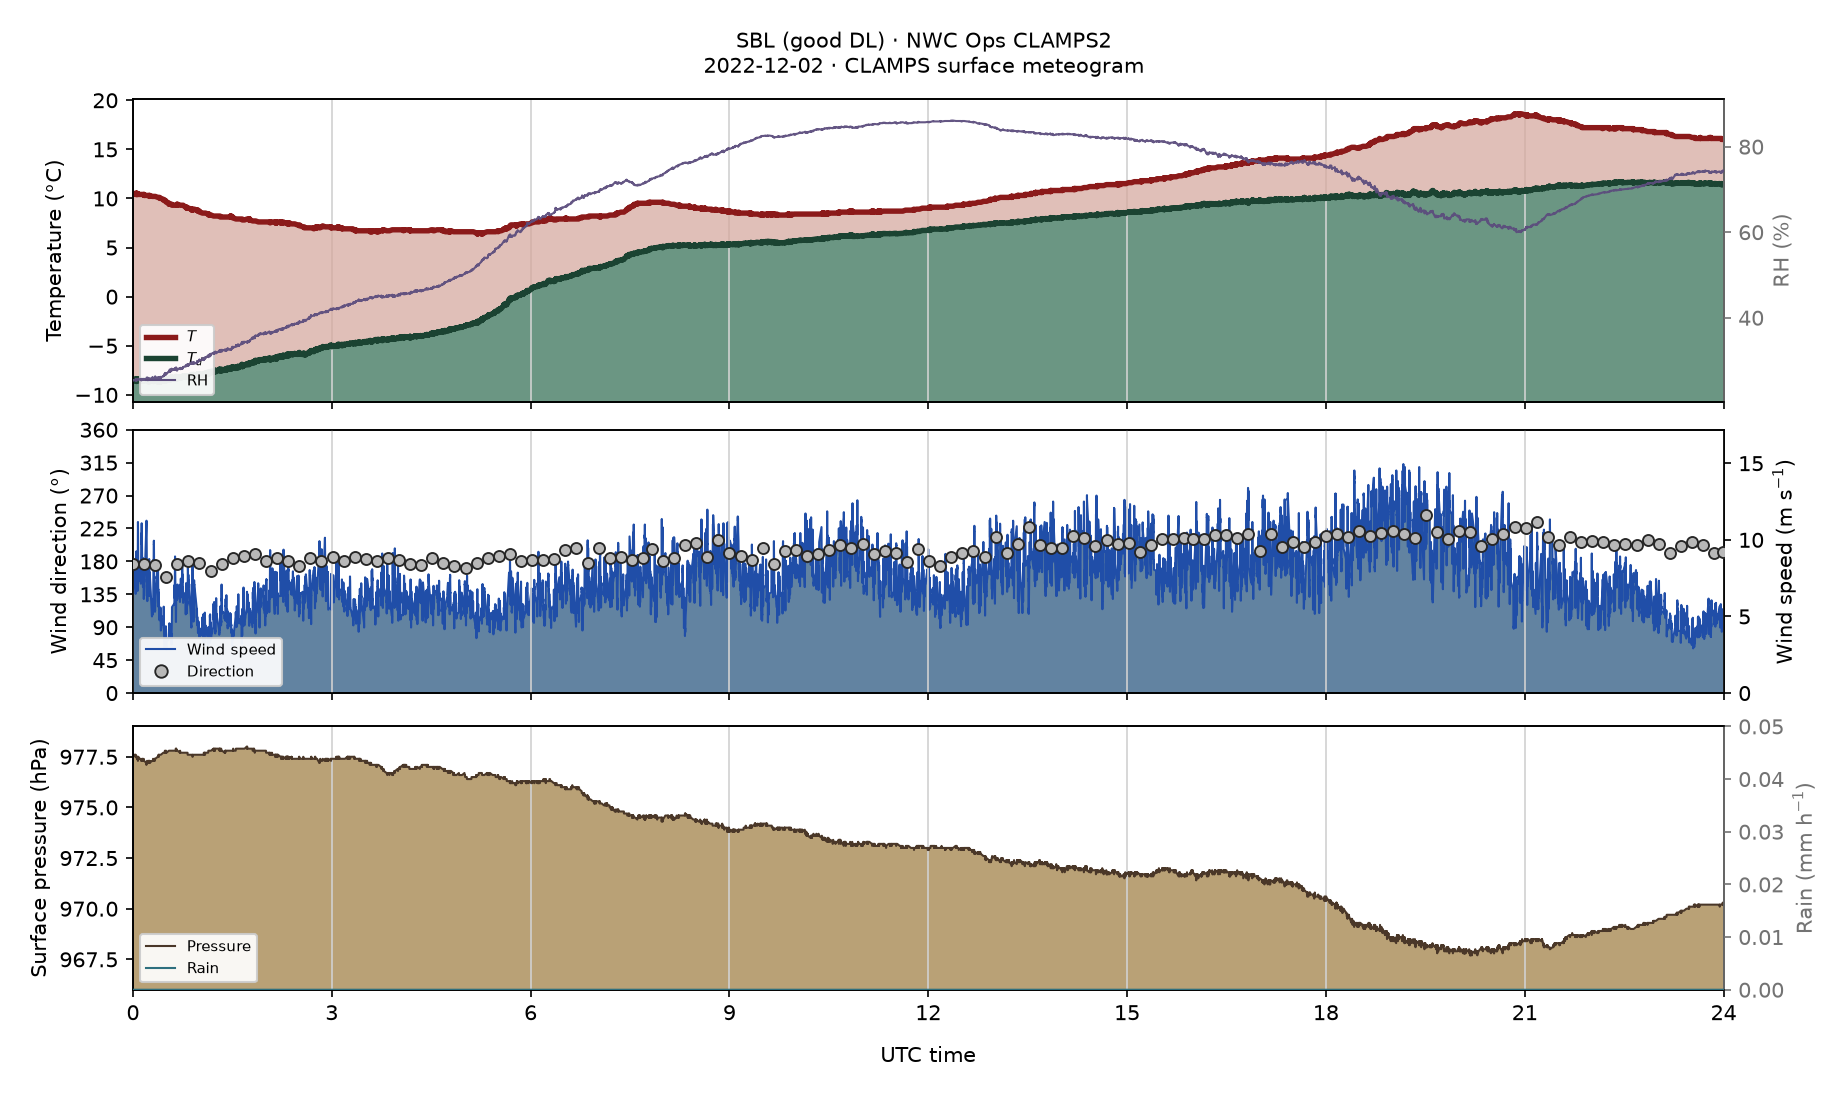
\includegraphics[width=0.92\textwidth]{../../images/stable_good_dl_c2_aux_surface_meteogram.png}
  \caption{Surface meteogram.
  Norman surface observations documenting sub-zero dewpoints, falling pressure, and the synoptic draw that sustains the high-velocity wind maximum.}
  \label{fig:stable_good_dl_c2:stable_good_dl_c2_aux_surface_meteogram}
\end{figure}
\section{Convection Initiation}
\textit{CLAMPS2 $\cdot$ AWAKEN $\cdot$ Orlando, OK $\cdot$ July 3, 2023 $\cdot$ convection, CI, CBL}

\begin{figure}[htbp]
  \centering
  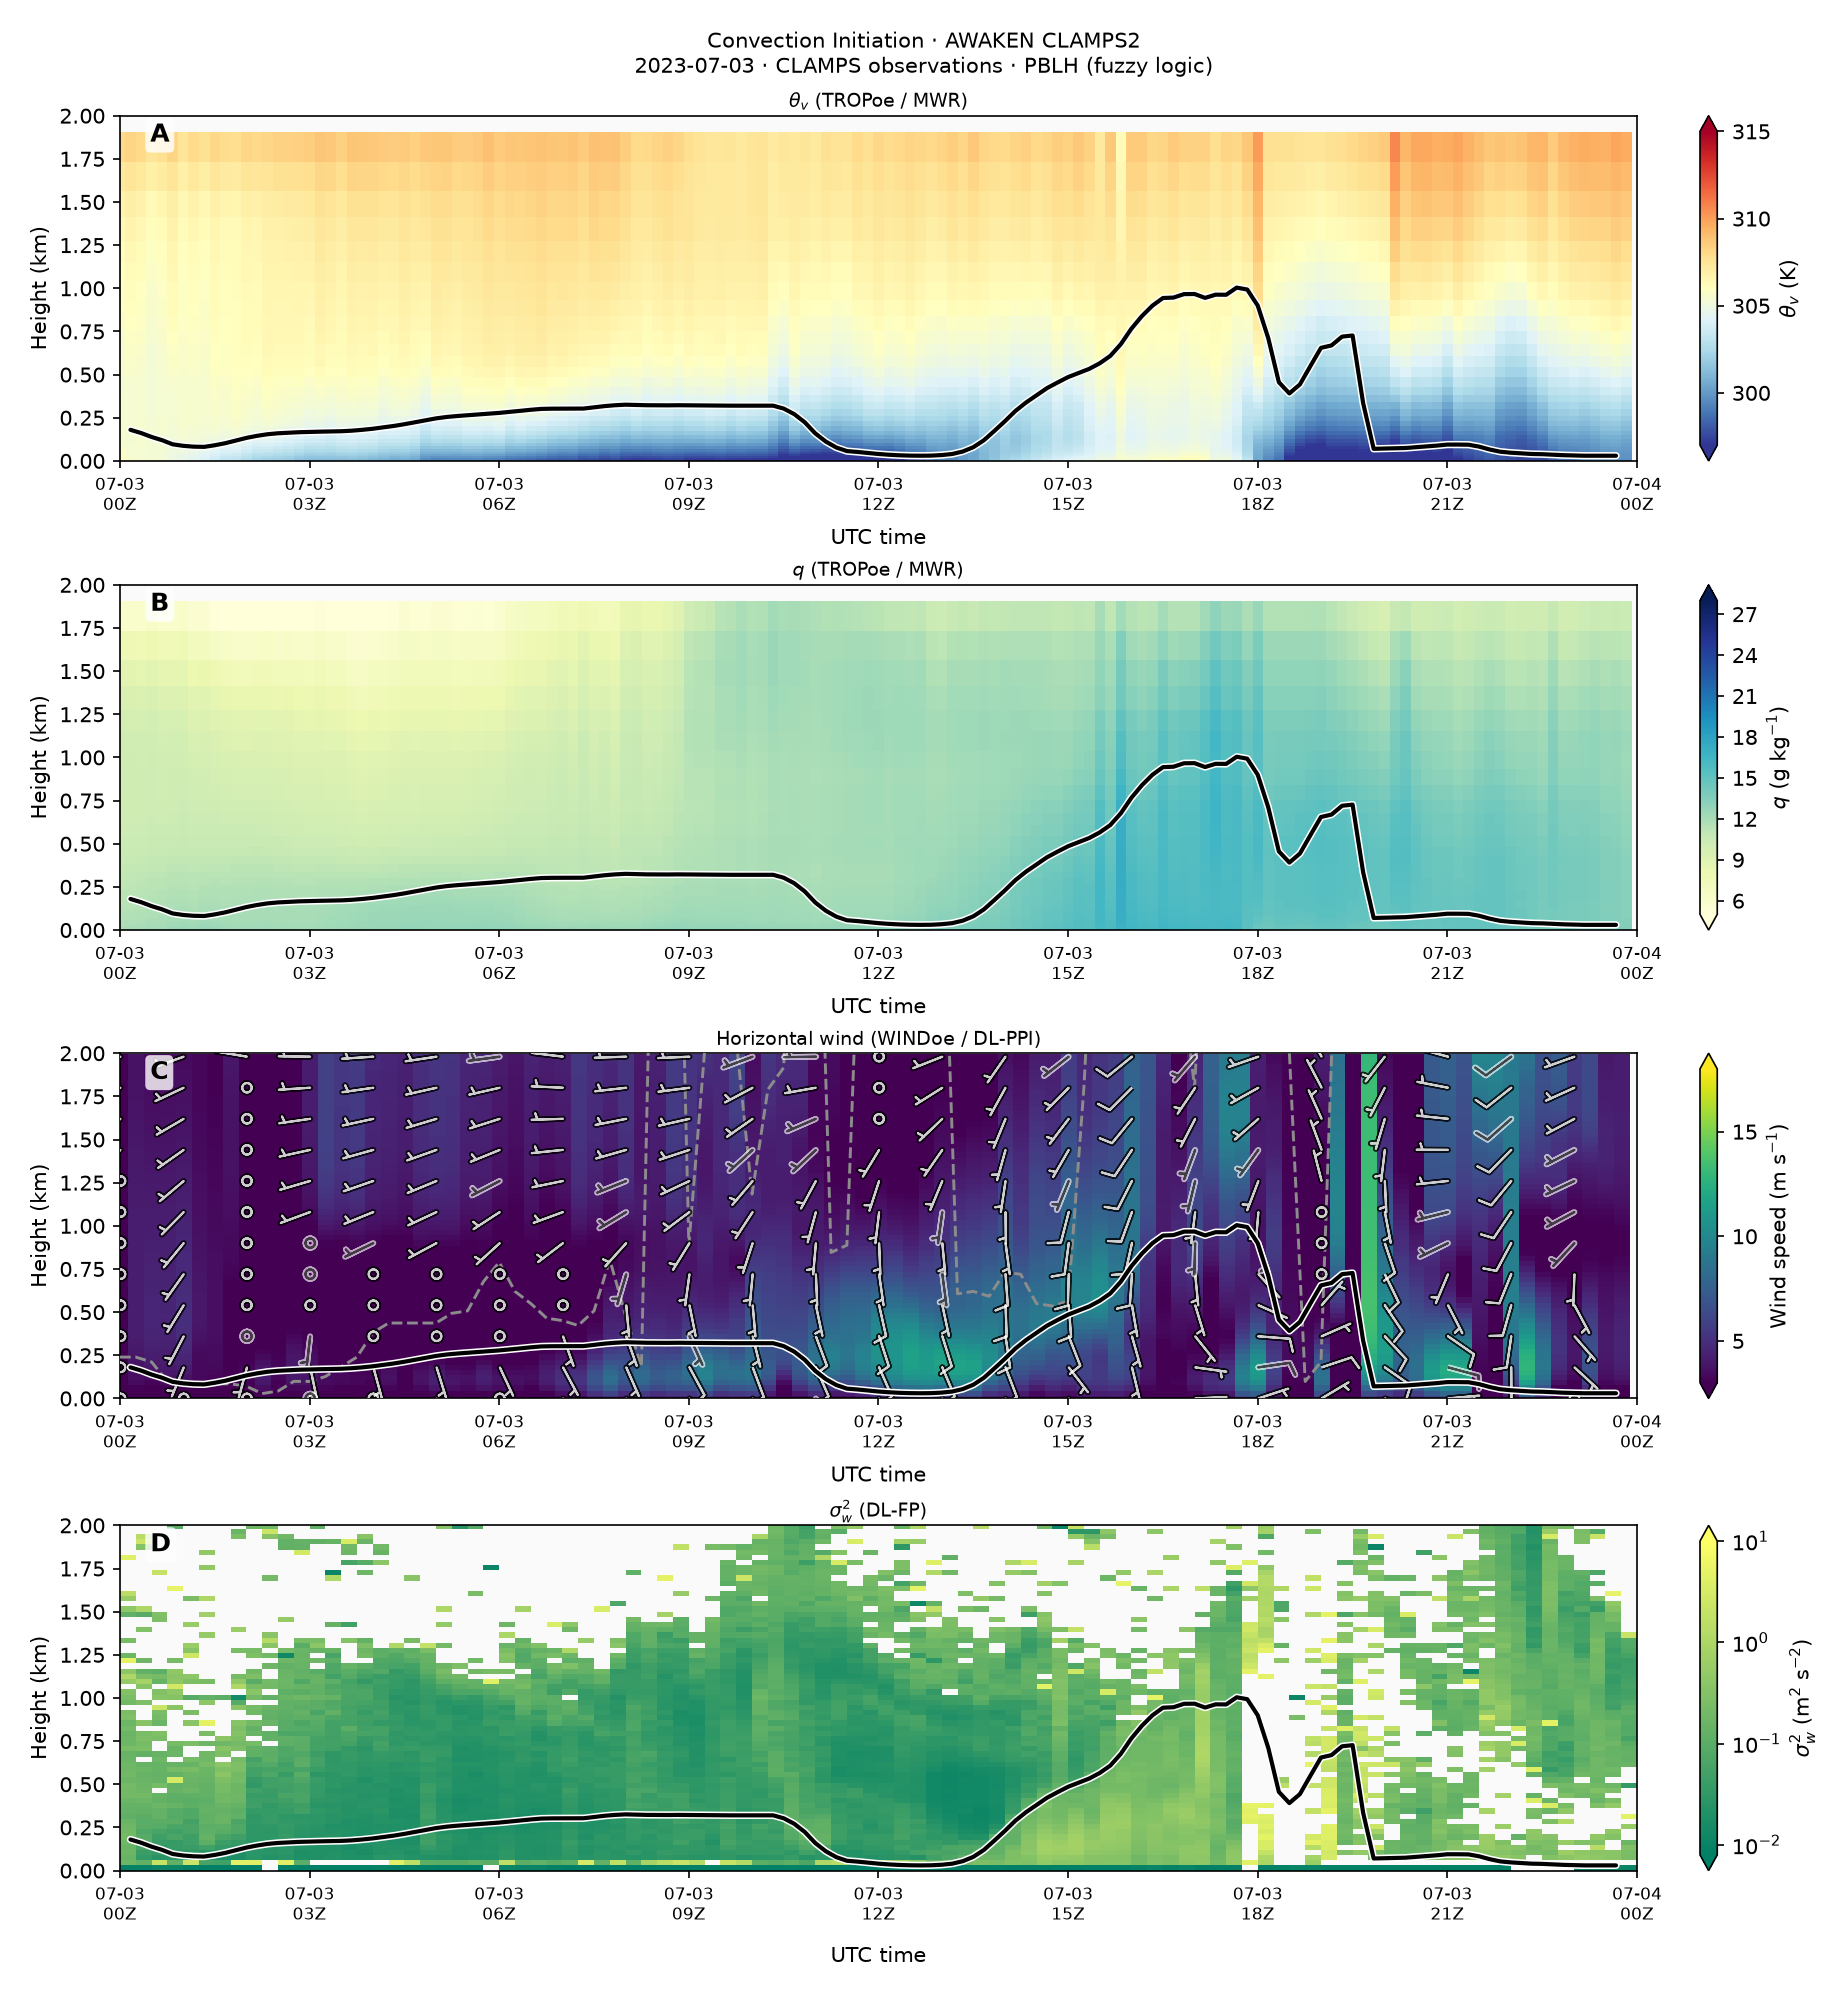
\includegraphics[width=\textwidth]{../../images/ci_c2_instrument_template_4panel.png}
  \caption{Standard CLAMPS observations.}
  \label{fig:ci_c2:ci_c2_instrument_template_4panel}
\end{figure}
\subsection*{Case overview}
This case from the AWAKEN campaign captures a pristine example of daytime convective boundary layer (CBL) growth, local convection initiation (CI), and a subsequent thunderstorm overpass. The first half of the period exhibits steady solar heating and well-behaved CBL growth that peaks near 1.0 km. Between 17:30 and 18:00 UTC, deep convection initiates and overruns the site. The storm's impact on the CLAMPS2 platform is clear, characterized by heavy precipitation that completely attenuates the Doppler lidar beam, kinematic shifting from convective downdrafts, and the arrival of a deep, surface-stabilizing convective cold pool.

\subsection*{Highlights}
\begin{itemize}
  \item CBL Growth \& Deep Post-Storm Cooling (Panel A): Steady solar insolation drives classic daytime boundary layer growth after 12:00 UTC, with the fuzzy-logic PBLH lifting cleanly to 1.0 km by 17:00 UTC in \hyperref[fig:ci_c2:ci_c2_instrument_template_4panel]{Standard CLAMPS observations}. At 18:00 UTC, the boundary layer is violently disrupted by the storm. Following a brief wave-like oscillation, a massive convective cold pool floods the lower atmosphere after 19:30 UTC, dropping virtual potential temperatures ($\theta_v$) below $300\text{ K}$ (deep blue shading) and completely pinning the PBL to the surface.
  \item Moisture Mixing \& Saturated Wake (Panel B): Ambient boundary layer moisture ($q \approx 12\text{ to }14\text{ g kg}^{-1}$) is efficiently mixed vertically through the 1.0 km column during afternoon destabilization in panel B of \hyperref[fig:ci_c2:ci_c2_instrument_template_4panel]{Standard CLAMPS observations}. The storm's arrival at 18:00 UTC introduces a sharp, fractured discontinuity in the water vapor field, followed by a deeply saturated, cool air mass that remains trapped under the cold pool inversion for the rest of the period.
  \item Convective Downbursts \& Outflow Shifting (Panel C): Moderate southerly and southwesterly flow characterizes the pristine daytime CBL. Right at 18:00 UTC, the wind field undergoes an intense disruption marked by a vertical column of accelerated wind speeds exceeding $15\text{ m s}^{-1}$ (bright yellow/green shading) and highly chaotic wind barbs, tracking the passage of a powerful convective downdraft and gust front. This arrival is dynamically validated at the surface by \hyperref[fig:ci_c2:ci_c2_aux_surface_meteogram]{Surface meteogram (precipitation)}, which records an instantaneous temperature crash from $31^\circ\text{C}$ down to $20^\circ\text{C}$, a sharp wind shift to the northwest, and an aggressive $6\text{ hPa}$ hydrostatic pressure jump (from 972 to 978 hPa).
  \item Precipitation Attenuation \& Signal Dropout (Panel D): The vertical velocity variance ($\sigma_w^2$) in panel D of \hyperref[fig:ci_c2:ci_c2_instrument_template_4panel]{Standard CLAMPS observations} beautifully highlights active thermal updrafts and downdrafts ($1\text{ to }10\text{ m}^2\text{ s}^{-2}$) expanding upward with the PBLH template. At exactly 18:00 UTC and again at 19:30 UTC, massive vertical white gaps obliterate the data stream across the entire 2.0 km column. This is the classic visual signature of heavy rainfall over the platform—corroborating the torrential core rain rate exceeding $110\text{ mm h}^{-1}$ logged in \hyperref[fig:ci_c2:ci_c2_aux_surface_meteogram]{Surface meteogram (precipitation)}—which completely attenuates the Doppler lidar's laser pulse and blocks data collection.
\end{itemize}
\begin{figure}[htbp]
  \centering
  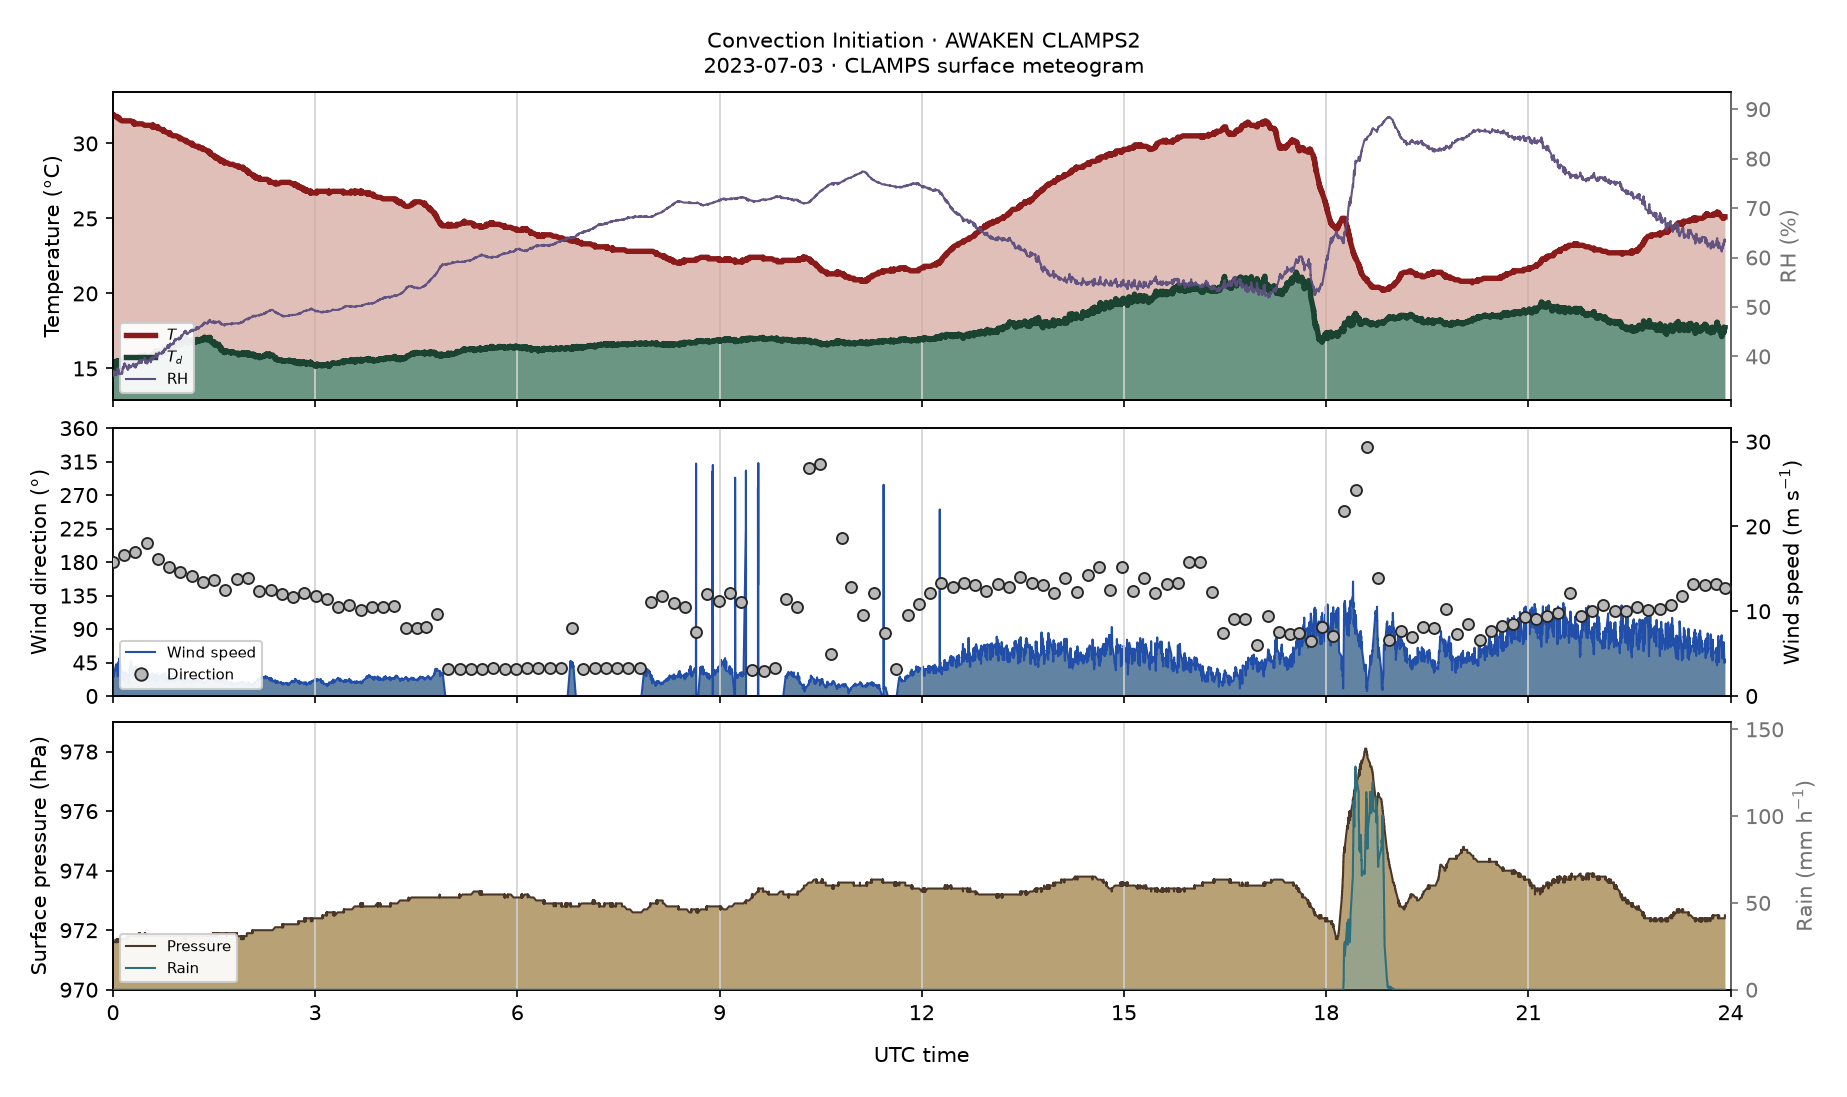
\includegraphics[width=0.92\textwidth]{../../images/ci_c2_aux_surface_meteogram.png}
  \caption{Surface meteogram (precipitation).
  Surface temperature, pressure, wind, and precipitation rate documenting storm arrival at 18:00 UTC, including core rain rates exceeding $110\,\mathrm{mm\,h^{-1}}$.}
  \label{fig:ci_c2:ci_c2_aux_surface_meteogram}
\end{figure}
\section{Gravity Waves}
\textit{CLAMPS2 $\cdot$ AWAKEN $\cdot$ Orlando, OK $\cdot$ August 5, 2023 $\cdot$ gravity waves, bore, boundaries, stable}

\begin{figure}[htbp]
  \centering
  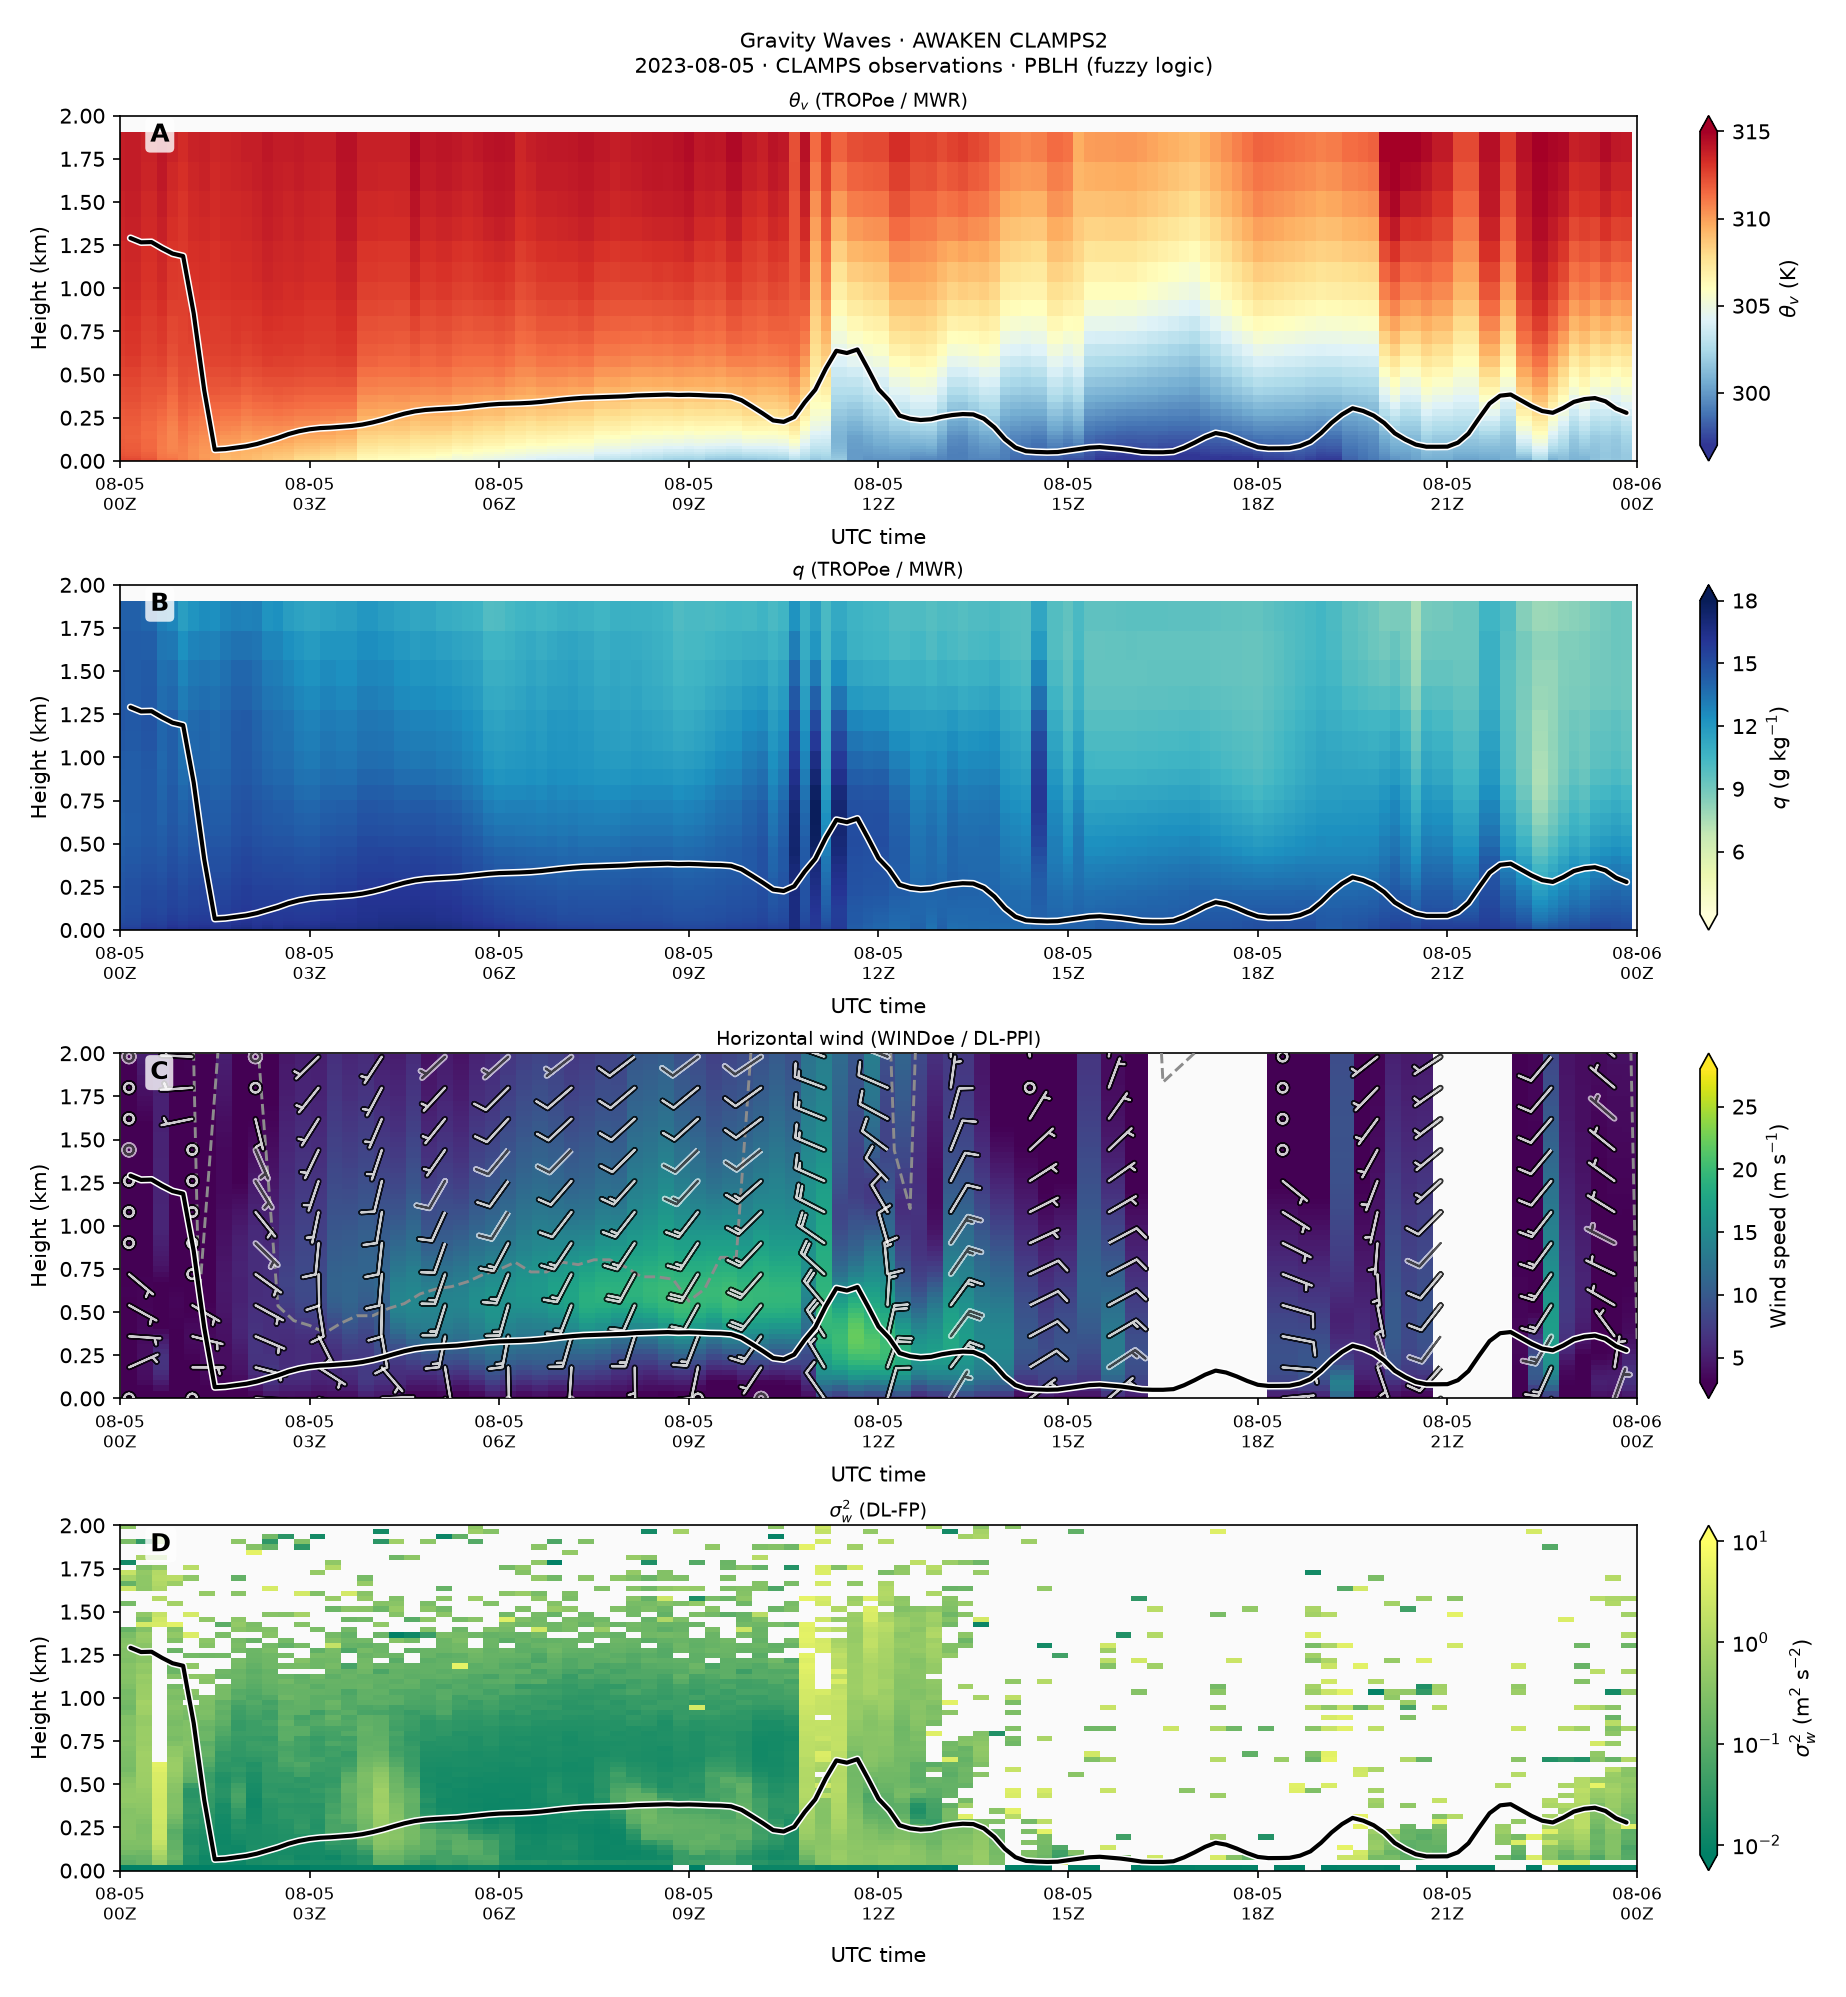
\includegraphics[width=\textwidth]{../../images/gravity_waves_c2_instrument_template_4panel.png}
  \caption{Standard CLAMPS observations.}
  \label{fig:gravity_waves_c2:gravity_waves_c2_instrument_template_4panel}
\end{figure}
\subsection*{Case overview}
This case from the AWAKEN campaign shows wave-driven boundary layer dynamics captured by the CLAMPS2 platform. The early part of the period features a steady, decoupling nocturnal boundary layer and a modest low-level jet. The highlight of the case occurs between 10:00 UTC and 20:00 UTC, when the atmosphere supports the generation and propagation of highly coherent wave features. This includes a sharp, solitary bore-like lifting event near 11:00 UTC, followed by an extended period of deep, long-period wave undulations that heavily modulate the thermal and moisture structure of the lower 1.25 km of the atmosphere.

\subsection*{Highlights}
\begin{itemize}
  \item Bore Passage \& Deep Undulations (Panel A): Prior to 10:00 UTC, a shallow stable layer is confined below 250 m. At 11:00 UTC, a classic atmospheric bore or solitary wave sharply lifts this stable layer, causing the fuzzy-logic planetary boundary layer height (PBLH) to surge up to \textasciitilde{}0.65 km before dropping back down. Following 14:00 UTC, a massive, long-period gravity wave train takes over, characterized by dramatic cooling ($\theta_v < 300\text{ K}$, blue shading) that stretches up to 1.25 km and undergoes deep, periodic vertical oscillations before flattening out after 20:00 UTC.
  \item Moisture Boundary Coherence (Panel B): The specific humidity ($q$) field acts as a highly passive tracer that maps the wave features perfectly. The sharp vertical spike at 11:00 UTC matches the initial bore crest. During the afternoon gravity wave event (14:00–19:00 UTC), a distinct dry air mass ($q \approx 6\text{ to }8\text{ g kg}^{-1}$, light green) is advected near the surface, with its upper boundary oscillating in perfect lockstep with the thermal wave crests and troughs aloft.
  \item Kinematic Reorganization \& Wind Maximum (Panel C): A nocturnal low-level jet with south-southwesterly winds peaking near $15\text{ m s}^{-1}$ is observed around 0.5 km between 06:00 UTC and 10:00 UTC. The arrival of the wave features completely disrupts this regime. Post-13:00 UTC, the wind profile undergoes a severe directional shift, transitioning to strong northeasterly/easterly flow aloft ($>15\text{ m s}^{-1}$) that rides over the undulating near-surface stable layer.
  \item Wave-Phased Turbulence Bursts (Panel D): The Doppler Lidar vertical velocity variance ($\sigma_w^2$) highlights how these laminar wave features interact with atmospheric shear. A distinct, localized burst of enhanced turbulence marks the nose of the initial bore at 11:00 UTC. Throughout the afternoon wave train, turbulence remains largely suppressed within the core of the cold pool, but exhibits intermittent, periodic enhancements aloft that align with the shear zones generated by the passing wave tilts.
\end{itemize}
\begin{figure}[htbp]
  \centering
  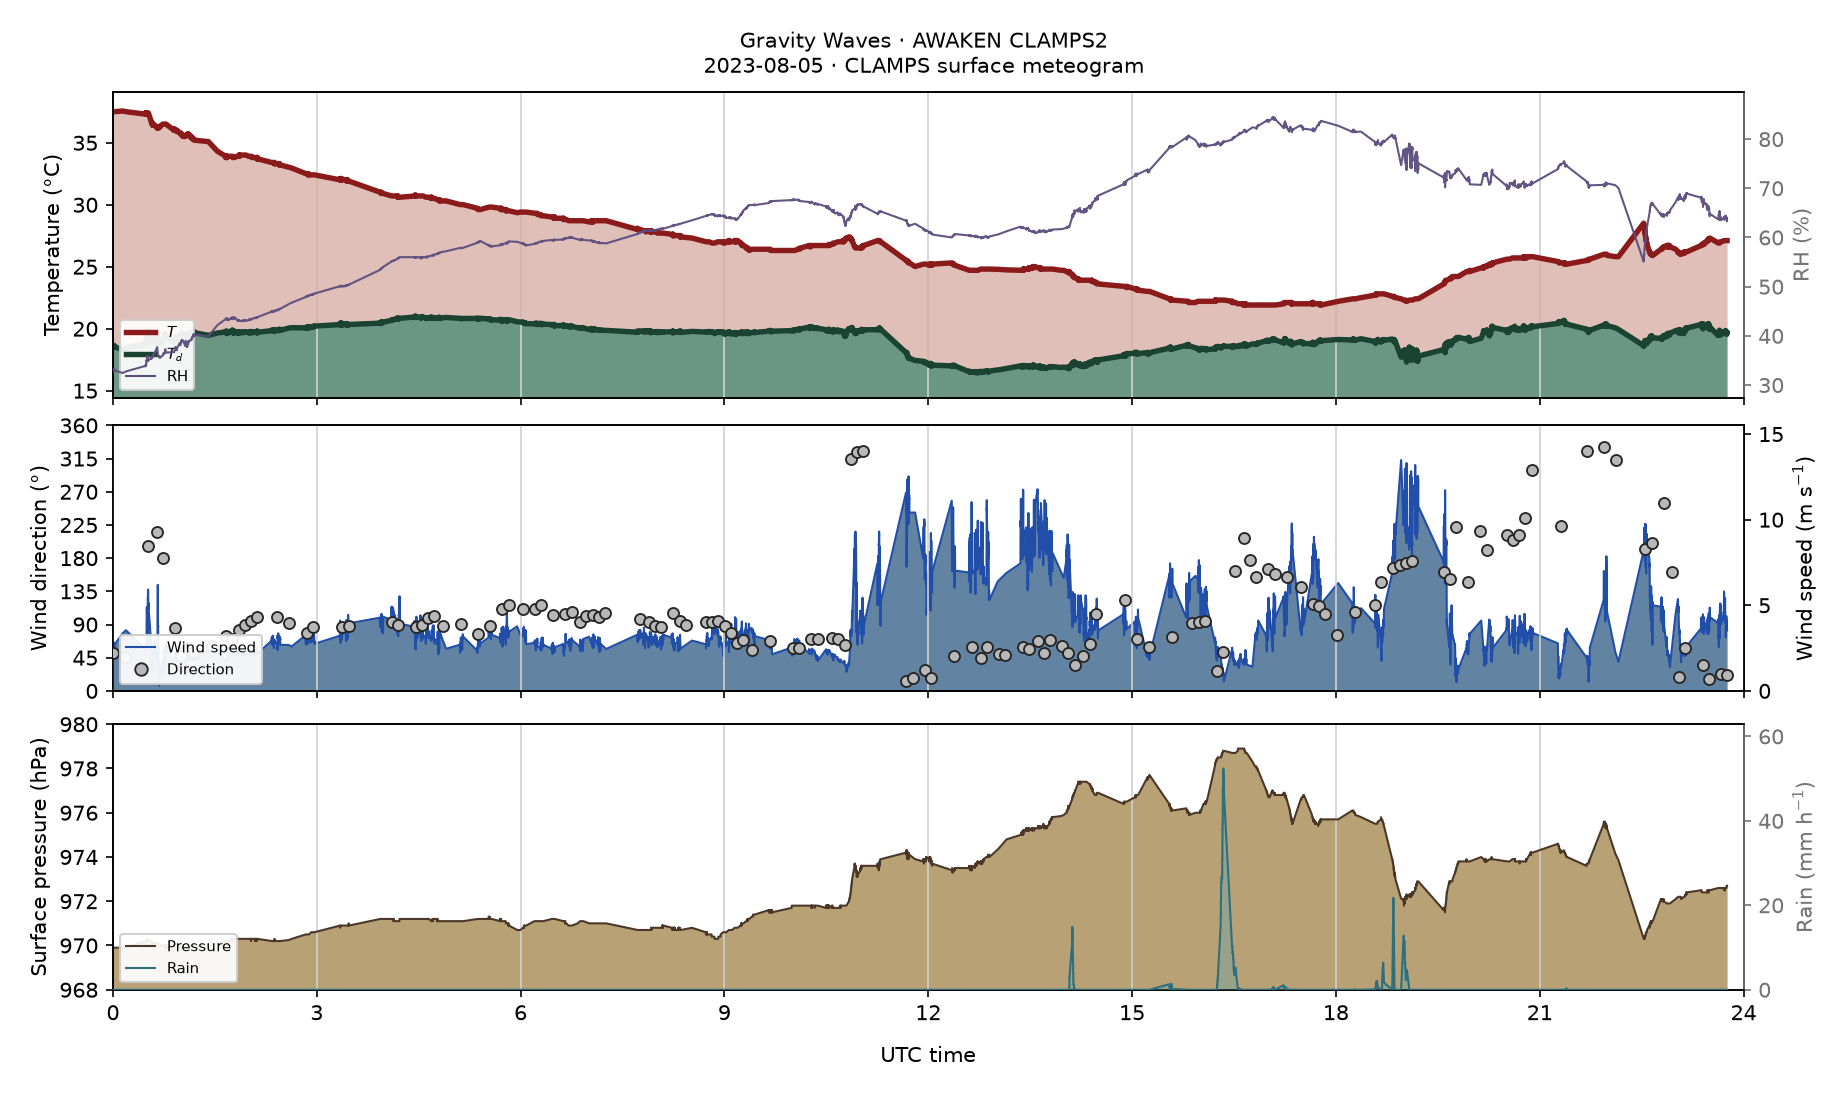
\includegraphics[width=0.92\textwidth]{../../images/gravity_waves_c2_aux_surface_meteogram.png}
  \caption{Surface meteogram (full day).
  Full-period surface meteogram providing thermodynamic and kinematic context for the nocturnal jet, bore passage, and afternoon wave train.}
  \label{fig:gravity_waves_c2:gravity_waves_c2_aux_surface_meteogram}
\end{figure}
\begin{figure}[htbp]
  \centering
  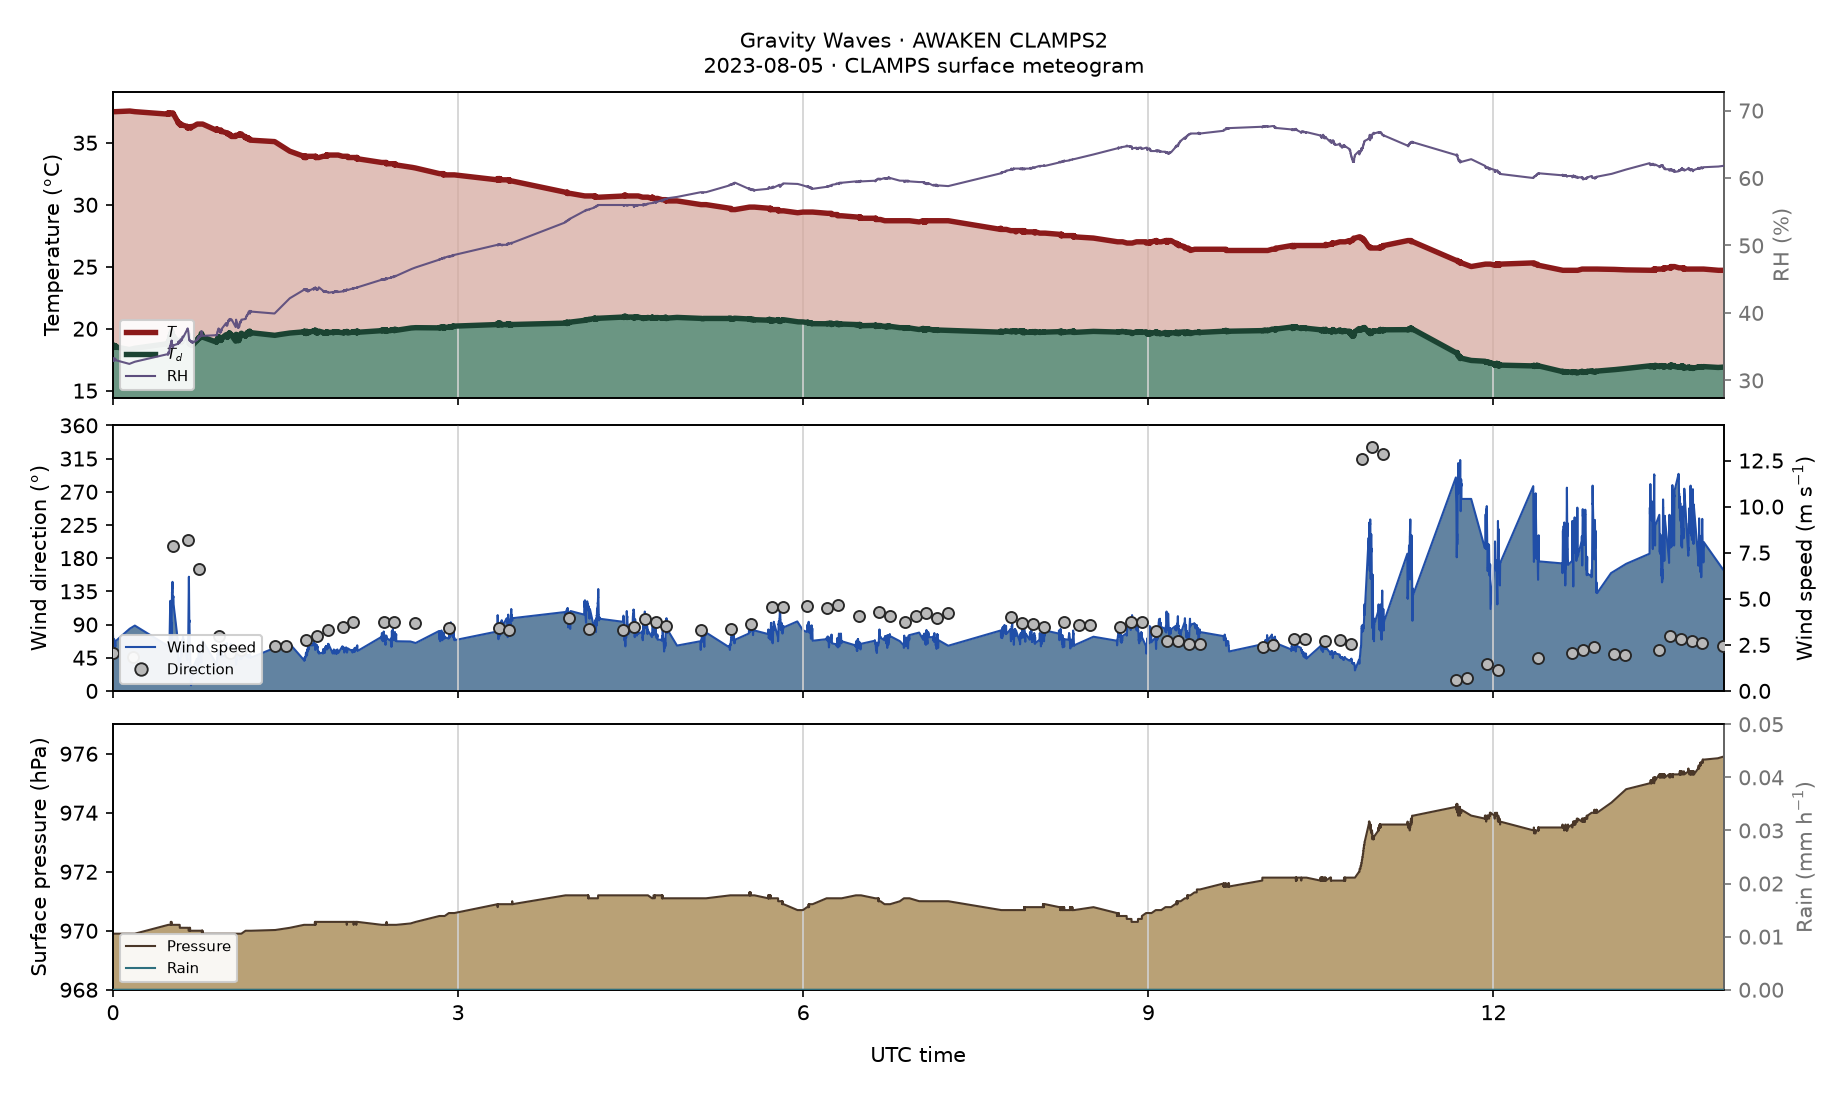
\includegraphics[width=0.92\textwidth]{../../images/gravity_waves_c2_aux_surface_meteogram_0_14.png}
  \caption{Surface meteogram (00–14 UTC).
  Morning subset (00–14 UTC) highlighting surface conditions during the solitary bore event near 11 UTC.}
  \label{fig:gravity_waves_c2:gravity_waves_c2_aux_surface_meteogram_0_14}
\end{figure}
\begin{figure}[htbp]
  \centering
  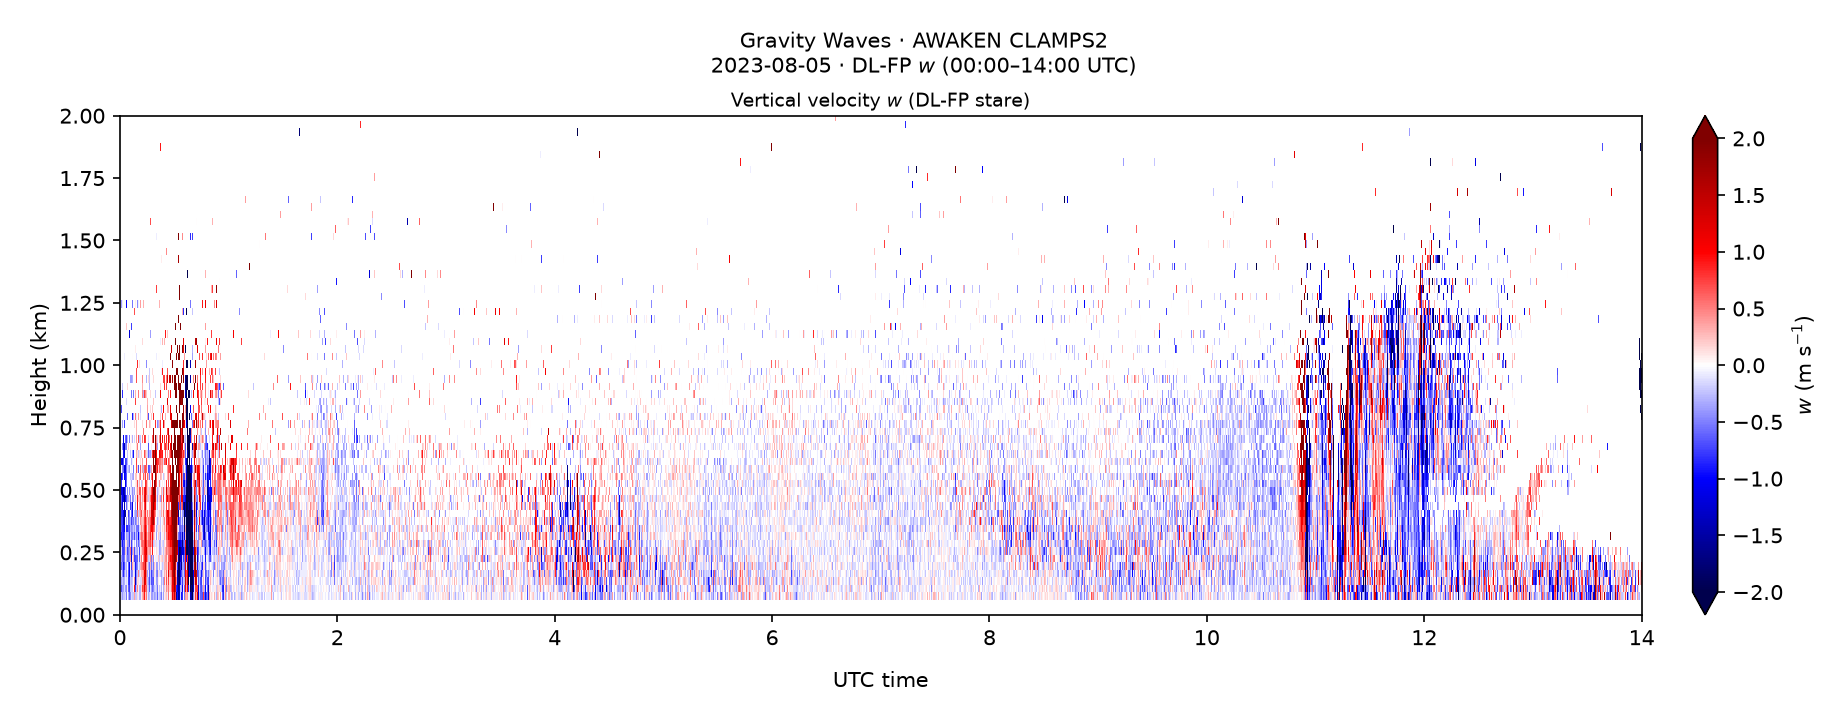
\includegraphics[width=0.92\textwidth]{../../images/gravity_waves_c2_aux_dlfp_w_timeheight.png}
  \caption{DL-FP vertical velocity (00–14 UTC).
  DL-FP vertical velocity (00–14 UTC) resolving laminar wave structures and the localized turbulent burst at the bore nose.}
  \label{fig:gravity_waves_c2:gravity_waves_c2_aux_dlfp_w_timeheight}
\end{figure}
\begin{figure}[htbp]
  \centering
  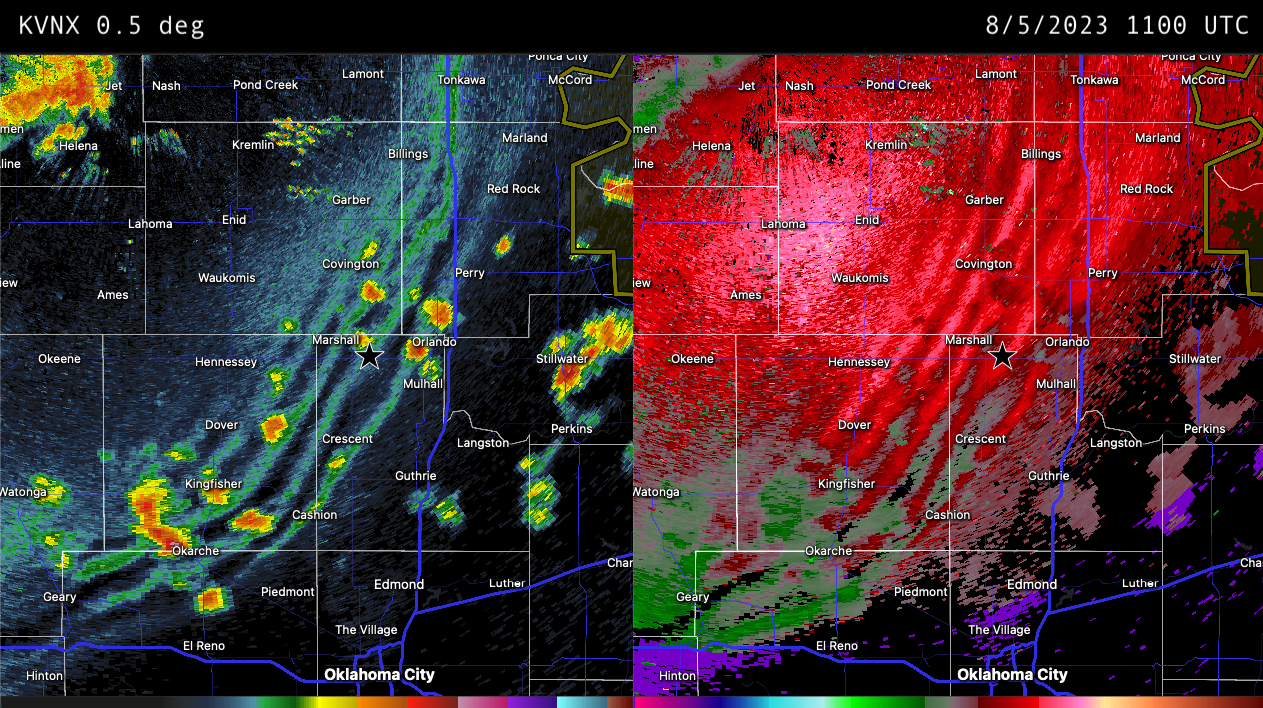
\includegraphics[width=0.92\textwidth]{../../images/gravity_waves_c2_88d_20230805_1100.png}
  \caption{NEXRAD 88D reflectivity (11 UTC).
  KTLX 88D reflectivity at 11 UTC showing regional convective and mesoscale structure associated with the wave-generating environment.}
  \label{fig:gravity_waves_c2:gravity_waves_c2_88d_20230805_1100}
\end{figure}
\section{Mature CBL}
\textit{CLAMPS2 $\cdot$ AWAKEN $\cdot$ Orlando, OK $\cdot$ August 25, 2023 $\cdot$ CBL, mature CBL}

\begin{figure}[htbp]
  \centering
  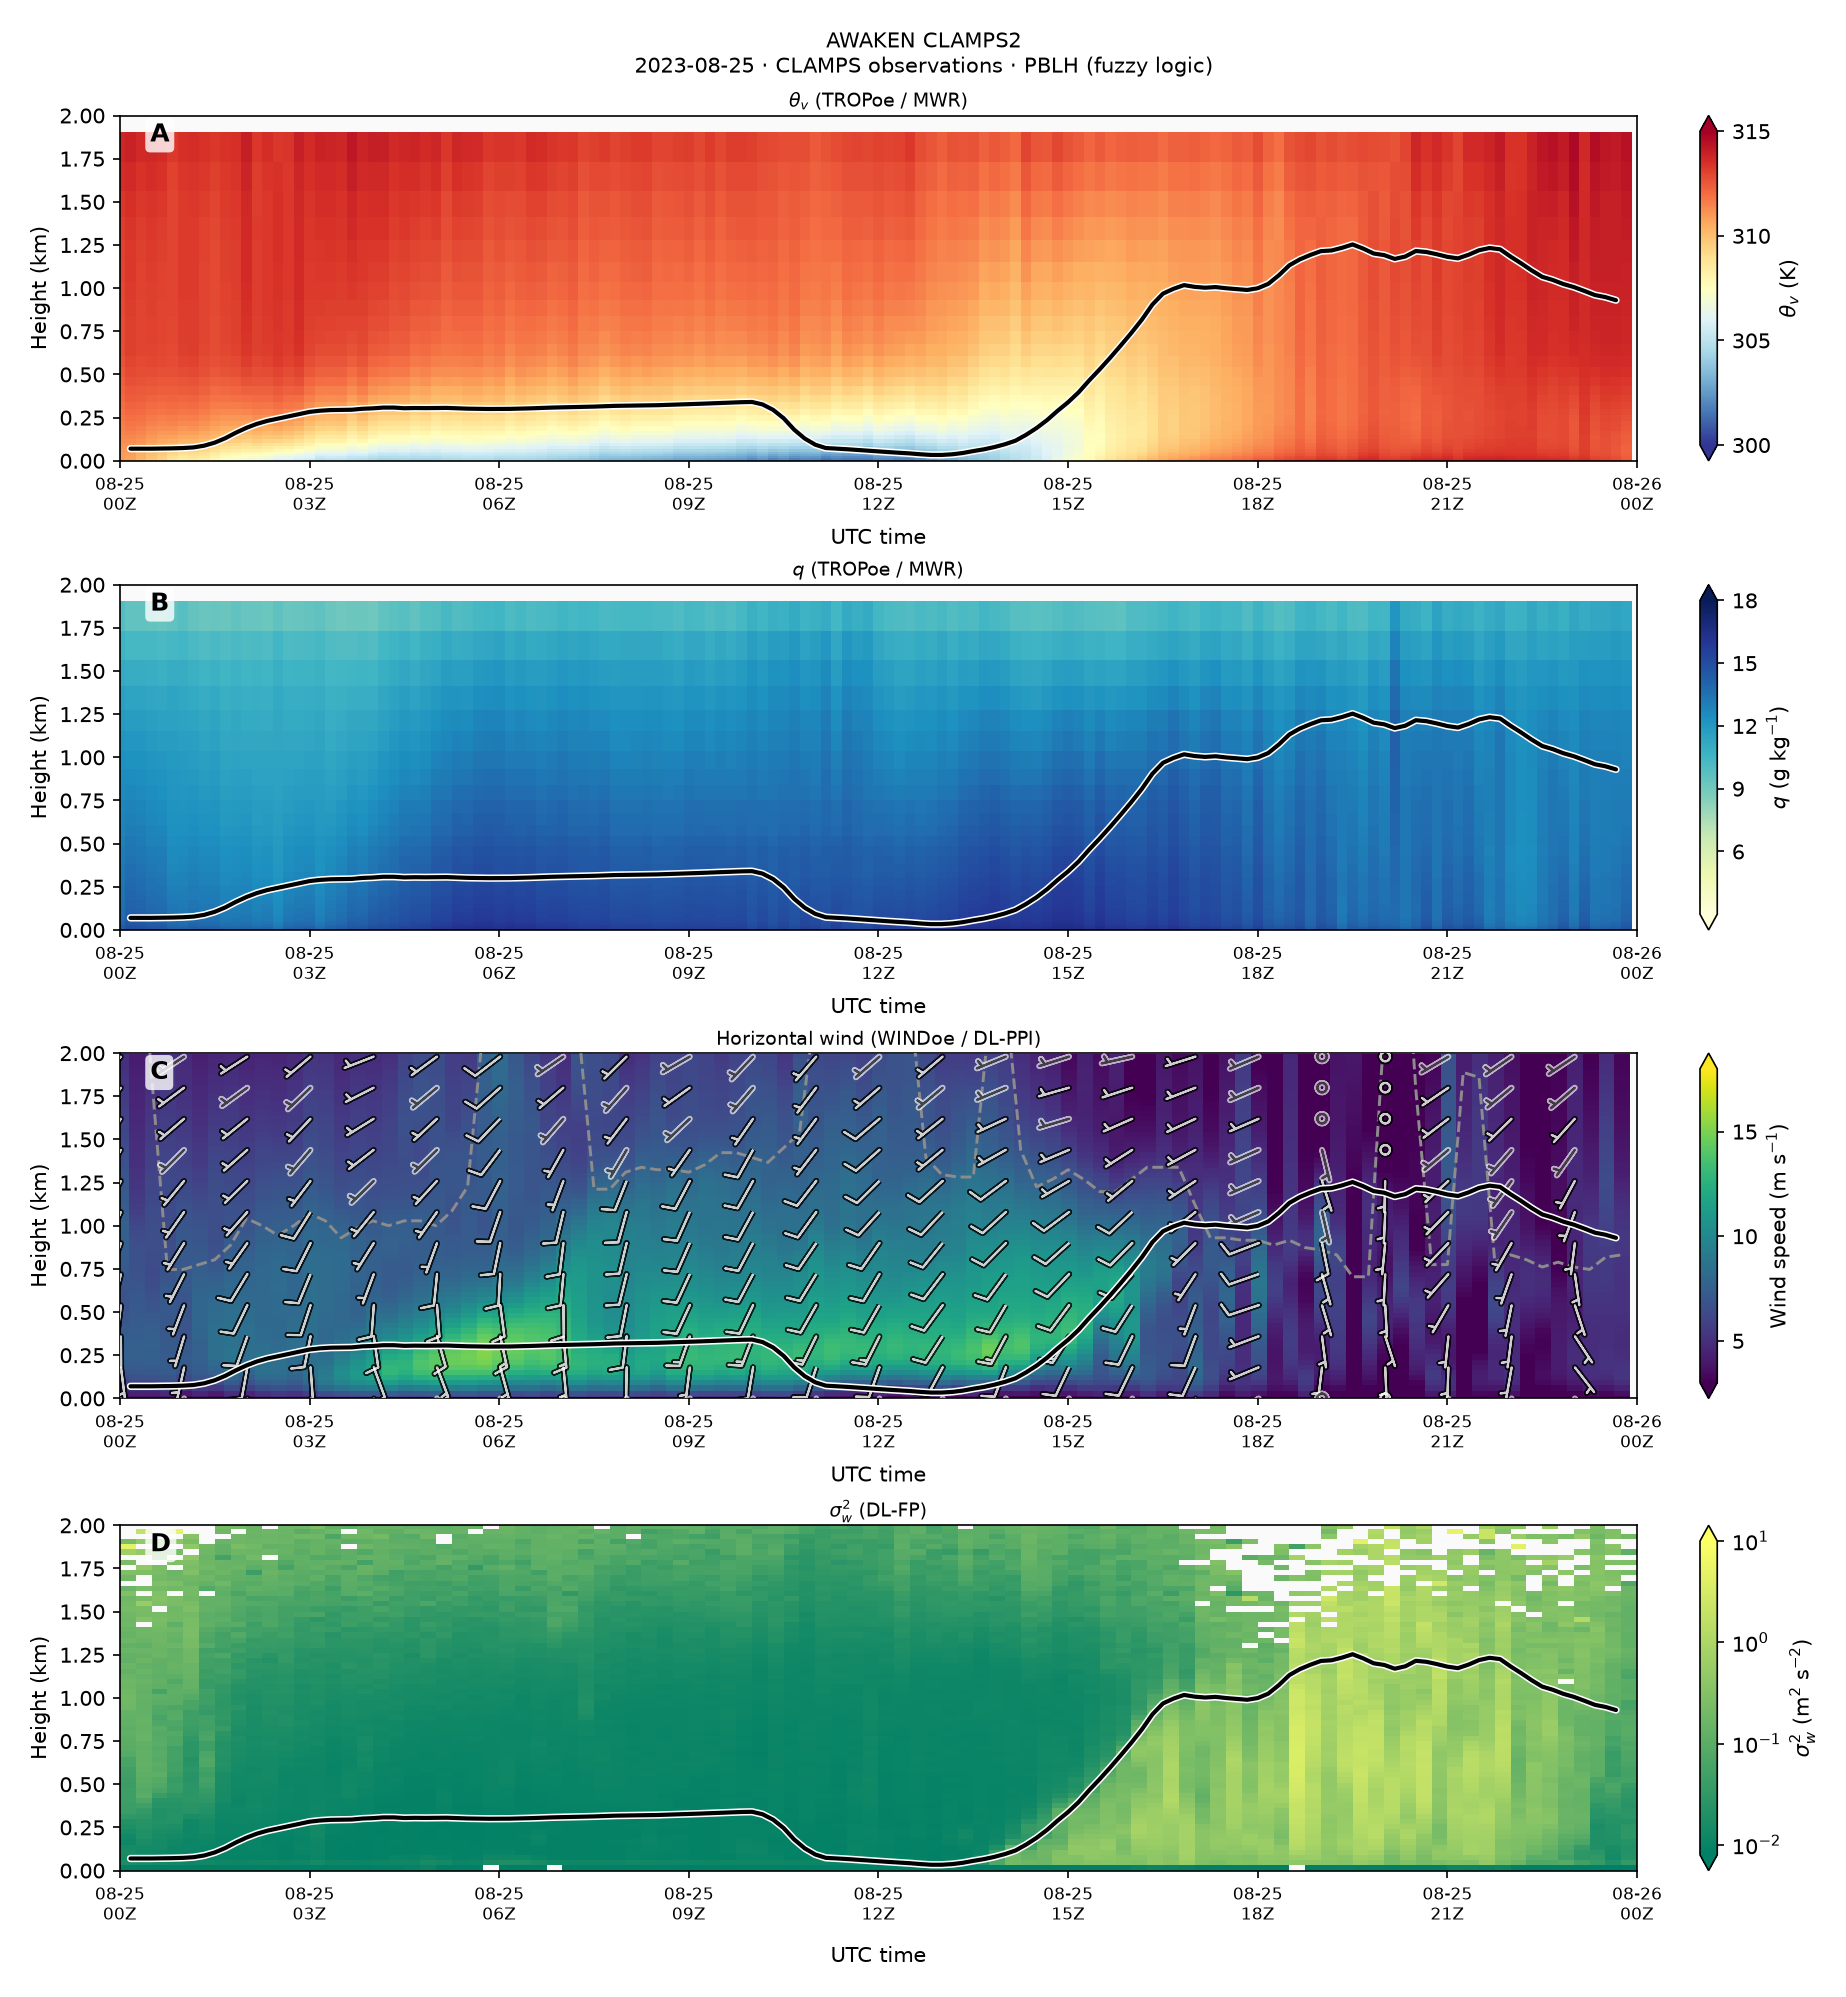
\includegraphics[width=\textwidth]{../../images/deep_cbl_c2_instrument_template_4panel.png}
  \caption{Standard CLAMPS observations.}
  \label{fig:deep_cbl_c2:deep_cbl_c2_instrument_template_4panel}
\end{figure}
\subsection*{Case overview}
This case study details the pristine, undisturbed lifecycle of a daytime Convective Boundary Layer (CBL) captured by the CLAMPS2 platform in northern Oklahoma. Following a highly stratified nocturnal regime, intense solar insulation rapidly erodes the morning inversion after 13:00 UTC. Driven by vigorous heating (e.g., surface buoyancy fluxes), the boundary layer grows steadily throughout the afternoon, with the planetary boundary layer height (PBLH) peaking between 1.0 km and 1.25 km. This environment serves as a textbook testbed for boundary layer similarity theory, showcasing a perfectly uniform dry-adiabatic mixed layer, coherent convective thermals, and vertical velocity variance profiles that precisely match empirical convective scaling laws.

\subsection*{Highlights}
\begin{itemize}
  \item Progressive Thermal Mixing (Panel A): The virtual potential temperature ($\theta_v$) profiles in panel A of \hyperref[fig:deep_cbl_c2:deep_cbl_c2_instrument_template_4panel]{Standard CLAMPS observations} display a clean transition from a shallow nocturnal stable layer to a deeply mixed convective column. By 18:00 UTC, sustained solar heating establishes a uniform mixed layer with temperatures exceeding 312 K. The automated PBLH line tracks a steady daytime expansion, stabilizing near 1.2 km through the late afternoon.
  \item Convective Momentum Drag (Panel C): In the afternoon (16:00 to 22:00 UTC), vigorous convective overturning efficiently mixes momentum vertically, causing horizontal wind speeds within the CBL to plunge below 5 m s$^{-1}$ (deep purple shading) in panel C of \hyperref[fig:deep_cbl_c2:deep_cbl_c2_instrument_template_4panel]{Standard CLAMPS observations}, leaving a calm, buoyancy-dominated environment.
  \item Convective Breakout Initiation: Prior to 14:00 UTC, vertical motions in the un-averaged vertical velocity staring scan of \hyperref[fig:deep_cbl_c2:deep_cbl_c2_aux_raw_w_timeheight]{Vertical velocity $w$ (DL-FP, 12–00 UTC)} are flat and laminar. As solar heating kicks in, narrow, surface-rooted updraft cores (red plumes) begin punching upward through the dissolving morning inversion layer.
  \item Textbook Convective Thermals: During peak heating, the column resolves a pristine display of alternating updraft (red) and downdraft (blue) structures in \hyperref[fig:deep_cbl_c2:deep_cbl_c2_aux_raw_w_timeheight]{Vertical velocity $w$ (DL-FP, 12–00 UTC)}. Core vertical velocities within the primary updraft plumes reach intense speeds of +2 to +3 m s$^{-1}$ between 19:00 UTC and 20:00 UTC.
  \item Visual PBL Top Verification: Notice how the vibrant red and blue plumes in \hyperref[fig:deep_cbl_c2:deep_cbl_c2_aux_raw_w_timeheight]{Vertical velocity $w$ (DL-FP, 12–00 UTC)} abruptly terminate at an altitude of exactly 1.2 km, turning into weak, unorganized motion aloft. This provides a direct, non-parameterized visual confirmation of the capping inversion base, aligning flawlessly with the automated fuzzy-logic line tracker in the master panels of \hyperref[fig:deep_cbl_c2:deep_cbl_c2_instrument_template_4panel]{Standard CLAMPS observations}.
  \item Surface Thermodynamic Forcing: Grounding the upper-air profiles, the surface observations in \hyperref[fig:deep_cbl_c2:deep_cbl_c2_aux_surface_meteogram]{Surface meteogram} capture the local weather trailing this deep mixing event. The top panel shows ambient surface temperatures climbing to a blistering 38.2$^{\circ}$C between 18:00 and 22:00 UTC, while the relative humidity (RH) plunges to 23\%, validating the intense sensible heat engine powering the midday thermal plumes.
  \item Mixed-Layer Growth Quantification: The midday 3-hour step-wise line plot in \hyperref[fig:deep_cbl_c2:deep_cbl_c2_aux_mixed_layer_profiles]{Midday $\theta_v$ and $q$ snapshots (15, 18, 21 UTC)} cleanly quantifies the growth of the mixed layer. By 18:00 UTC (solid black line) and 21:00 UTC (dashed line), the potential temperature and moisture profiles transform into perfectly vertical, homogeneous blocks from the surface up to the entrainment zone, verifying optimal boundary layer mixing efficiency.
  \item Peak-Heating Similarity Proof: A 1D snapshot profile at 18:30 UTC in \hyperref[fig:deep_cbl_c2:deep_cbl_c2_aux_sigma_w2_over_u_profile]{$\sigma_w^2 / w^{*2}$ and temperature snapshot (18:30 UTC)} mathematically anchors this case to classic fluid dynamics theory. When normalized by the convective velocity scale ($w^* = 1.32\text{ m s}^{-1}$), the empirical vertical velocity variance profile ($\sigma_w^2 / w^{*2}$) hits a maximum value of 0.44 at a physical height of 0.44 km. Evaluating this against the 1.2 km boundary layer ceiling yields a normalized height of maximum turbulent intensity: $\frac{z}{z_i} \approx 0.37$. Because empirical boundary layer scaling curves state that pure buoyant plumes maximize their vertical variance between a normalized height of 0.33 and 0.40, this profile serves as definitive proof that the CLAMPS2 platform can successfully map ideal boundary layer similarity mechanics.
\end{itemize}
\begin{figure}[htbp]
  \centering
  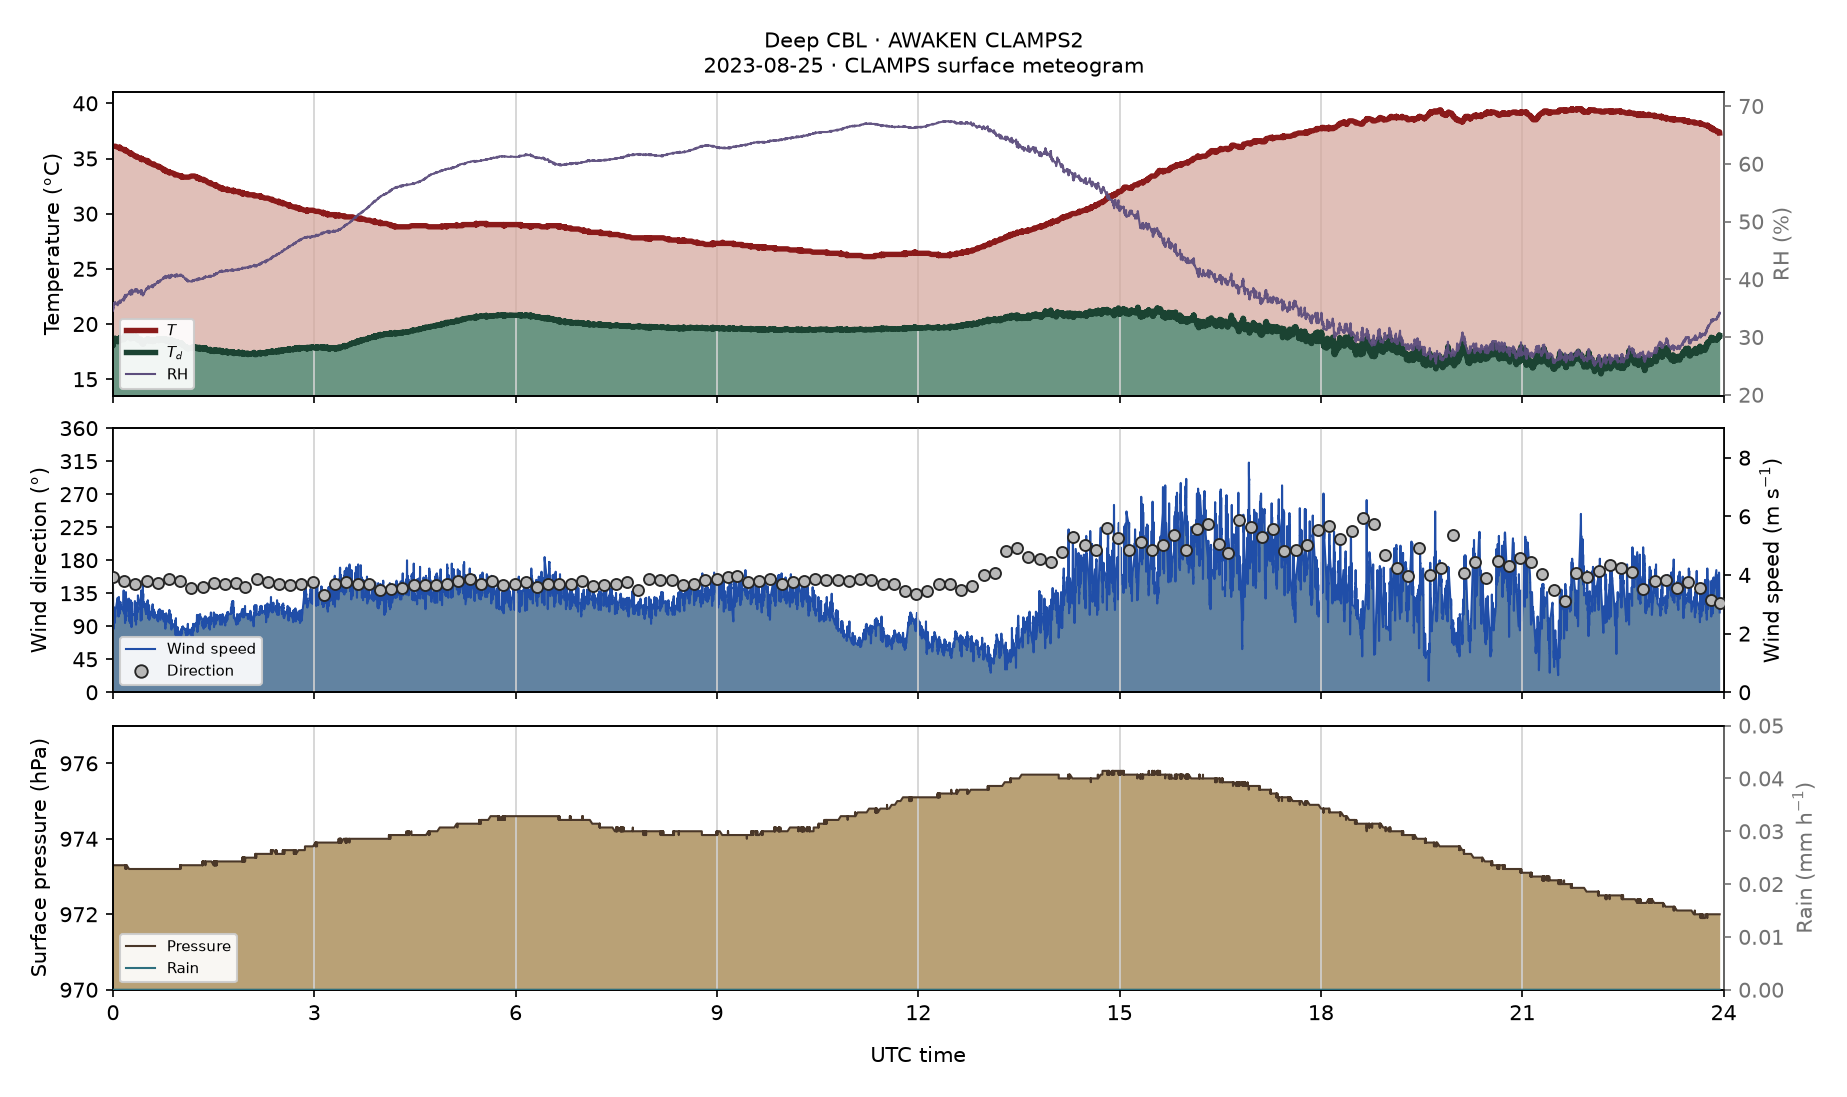
\includegraphics[width=0.92\textwidth]{../../images/deep_cbl_c2_aux_surface_meteogram.png}
  \caption{Surface meteogram.
  Surface temperature and relative humidity time series grounding the afternoon sensible-heating engine (peak $38.2^\circ\mathrm{C}$, RH $\rightarrow 23\%$) that drives convective thermals.}
  \label{fig:deep_cbl_c2:deep_cbl_c2_aux_surface_meteogram}
\end{figure}
\begin{figure}[htbp]
  \centering
  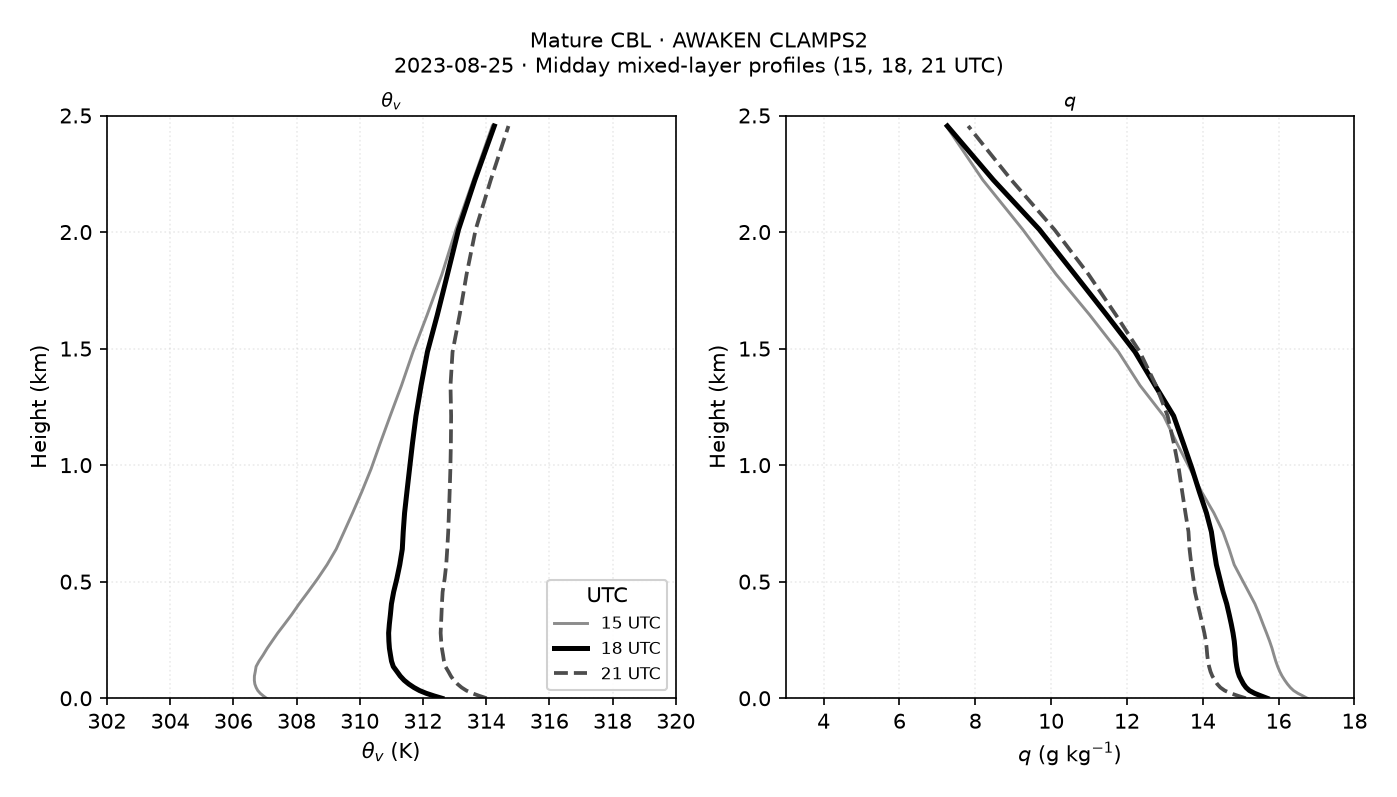
\includegraphics[width=0.92\textwidth]{../../images/deep_cbl_c2_aux_mixed_layer_profiles.png}
  \caption{Midday $\theta_v$ and $q$ snapshots (15, 18, 21 UTC).
  Midday $\theta_v$ and $q$ profile snapshots at 15, 18, and 21 UTC quantifying step-wise homogenization of the mixed layer.}
  \label{fig:deep_cbl_c2:deep_cbl_c2_aux_mixed_layer_profiles}
\end{figure}
\begin{figure}[htbp]
  \centering
  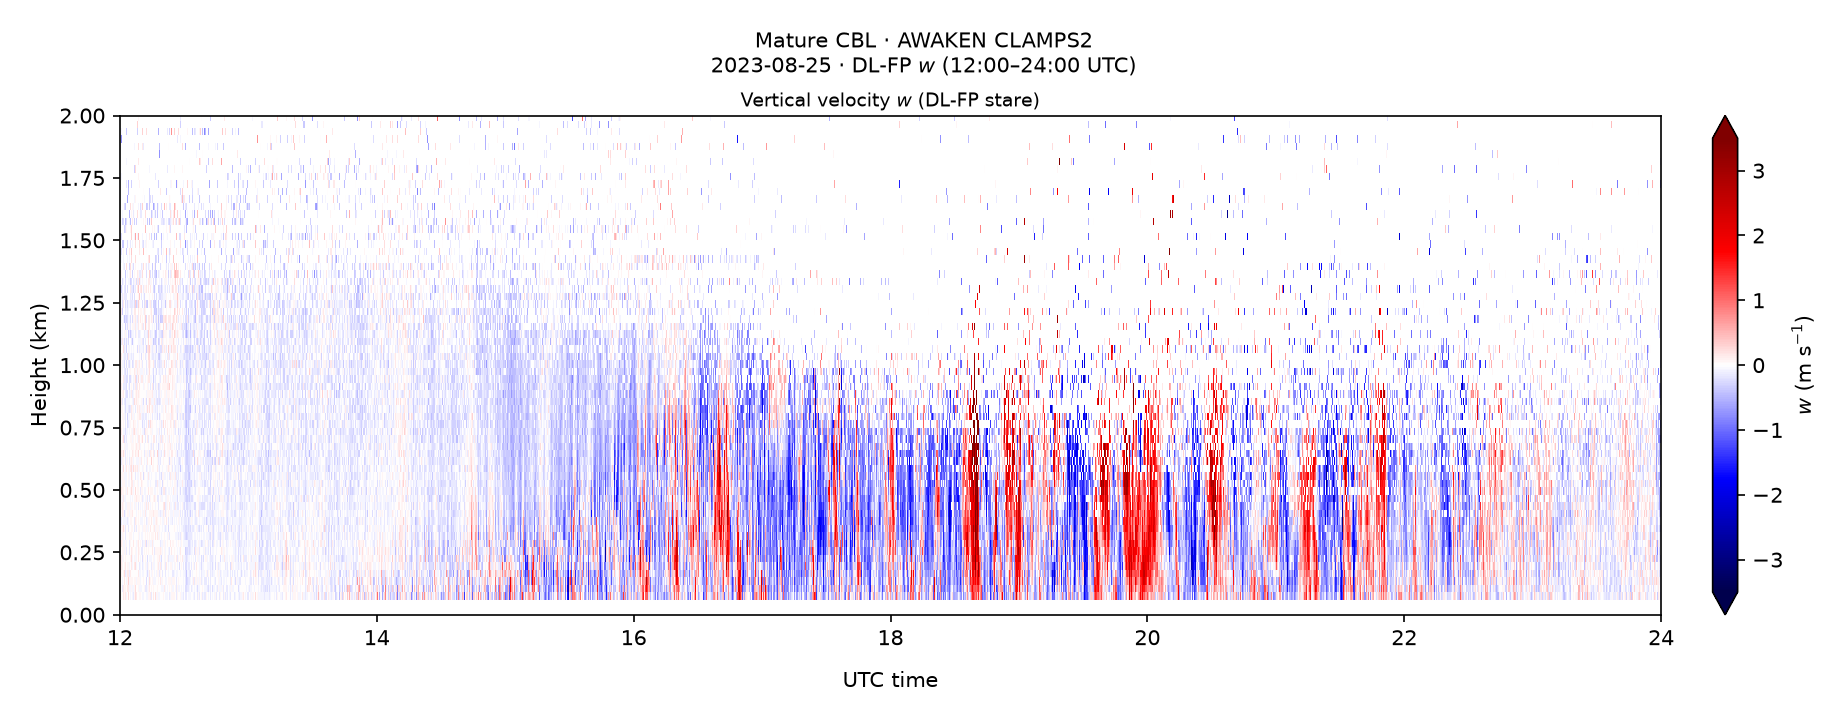
\includegraphics[width=0.92\textwidth]{../../images/deep_cbl_c2_aux_raw_w_timeheight.png}
  \caption{Vertical velocity $w$ (DL-FP, 12–00 UTC).
  Un-averaged DL-FP $w$ stare showing convective updraft and downdraft plumes that terminate abruptly at the $\sim$1.2 km capping inversion.}
  \label{fig:deep_cbl_c2:deep_cbl_c2_aux_raw_w_timeheight}
\end{figure}
\begin{figure}[htbp]
  \centering
  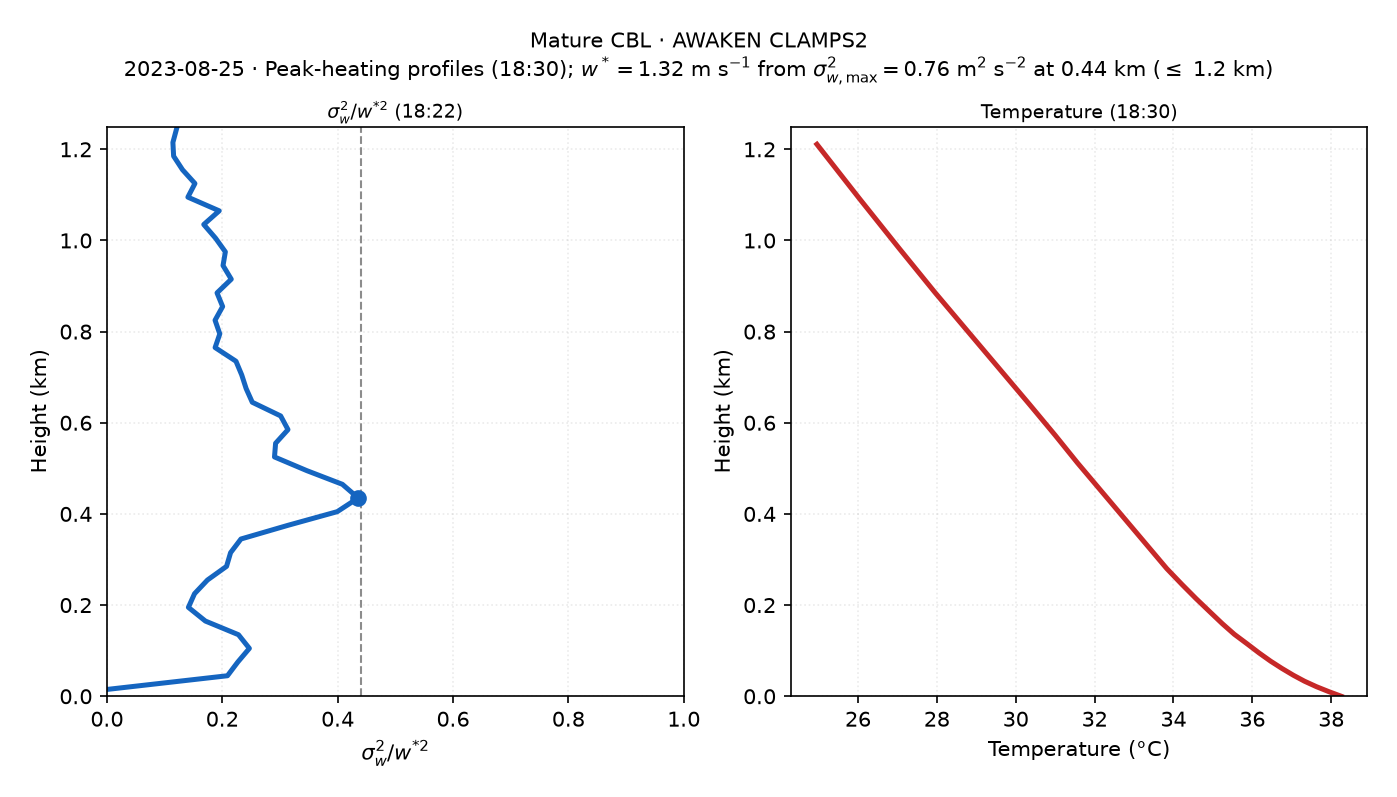
\includegraphics[width=0.92\textwidth]{../../images/deep_cbl_c2_aux_sigma_w2_over_U_profile.png}
  \caption{$\sigma_w^2 / w^{*2}$ and temperature snapshot (18:30 UTC).
  18:30 UTC profile snapshot comparing empirical $\sigma_w^2 / w^{*2}$ (maximum $\approx 0.44$ at $z/z_i \approx 0.37$) against convective similarity-theory expectations.}
  \label{fig:deep_cbl_c2:deep_cbl_c2_aux_sigma_w2_over_u_profile}
\end{figure}
\section{Land–Atmosphere Interaction}
\textit{CLAMPS1 $\cdot$ AWAKEN $\cdot$ Covington, OK $\cdot$ September 1, 2023 $\cdot$ land–atmosphere interaction, CBL}

\begin{figure}[htbp]
  \centering
  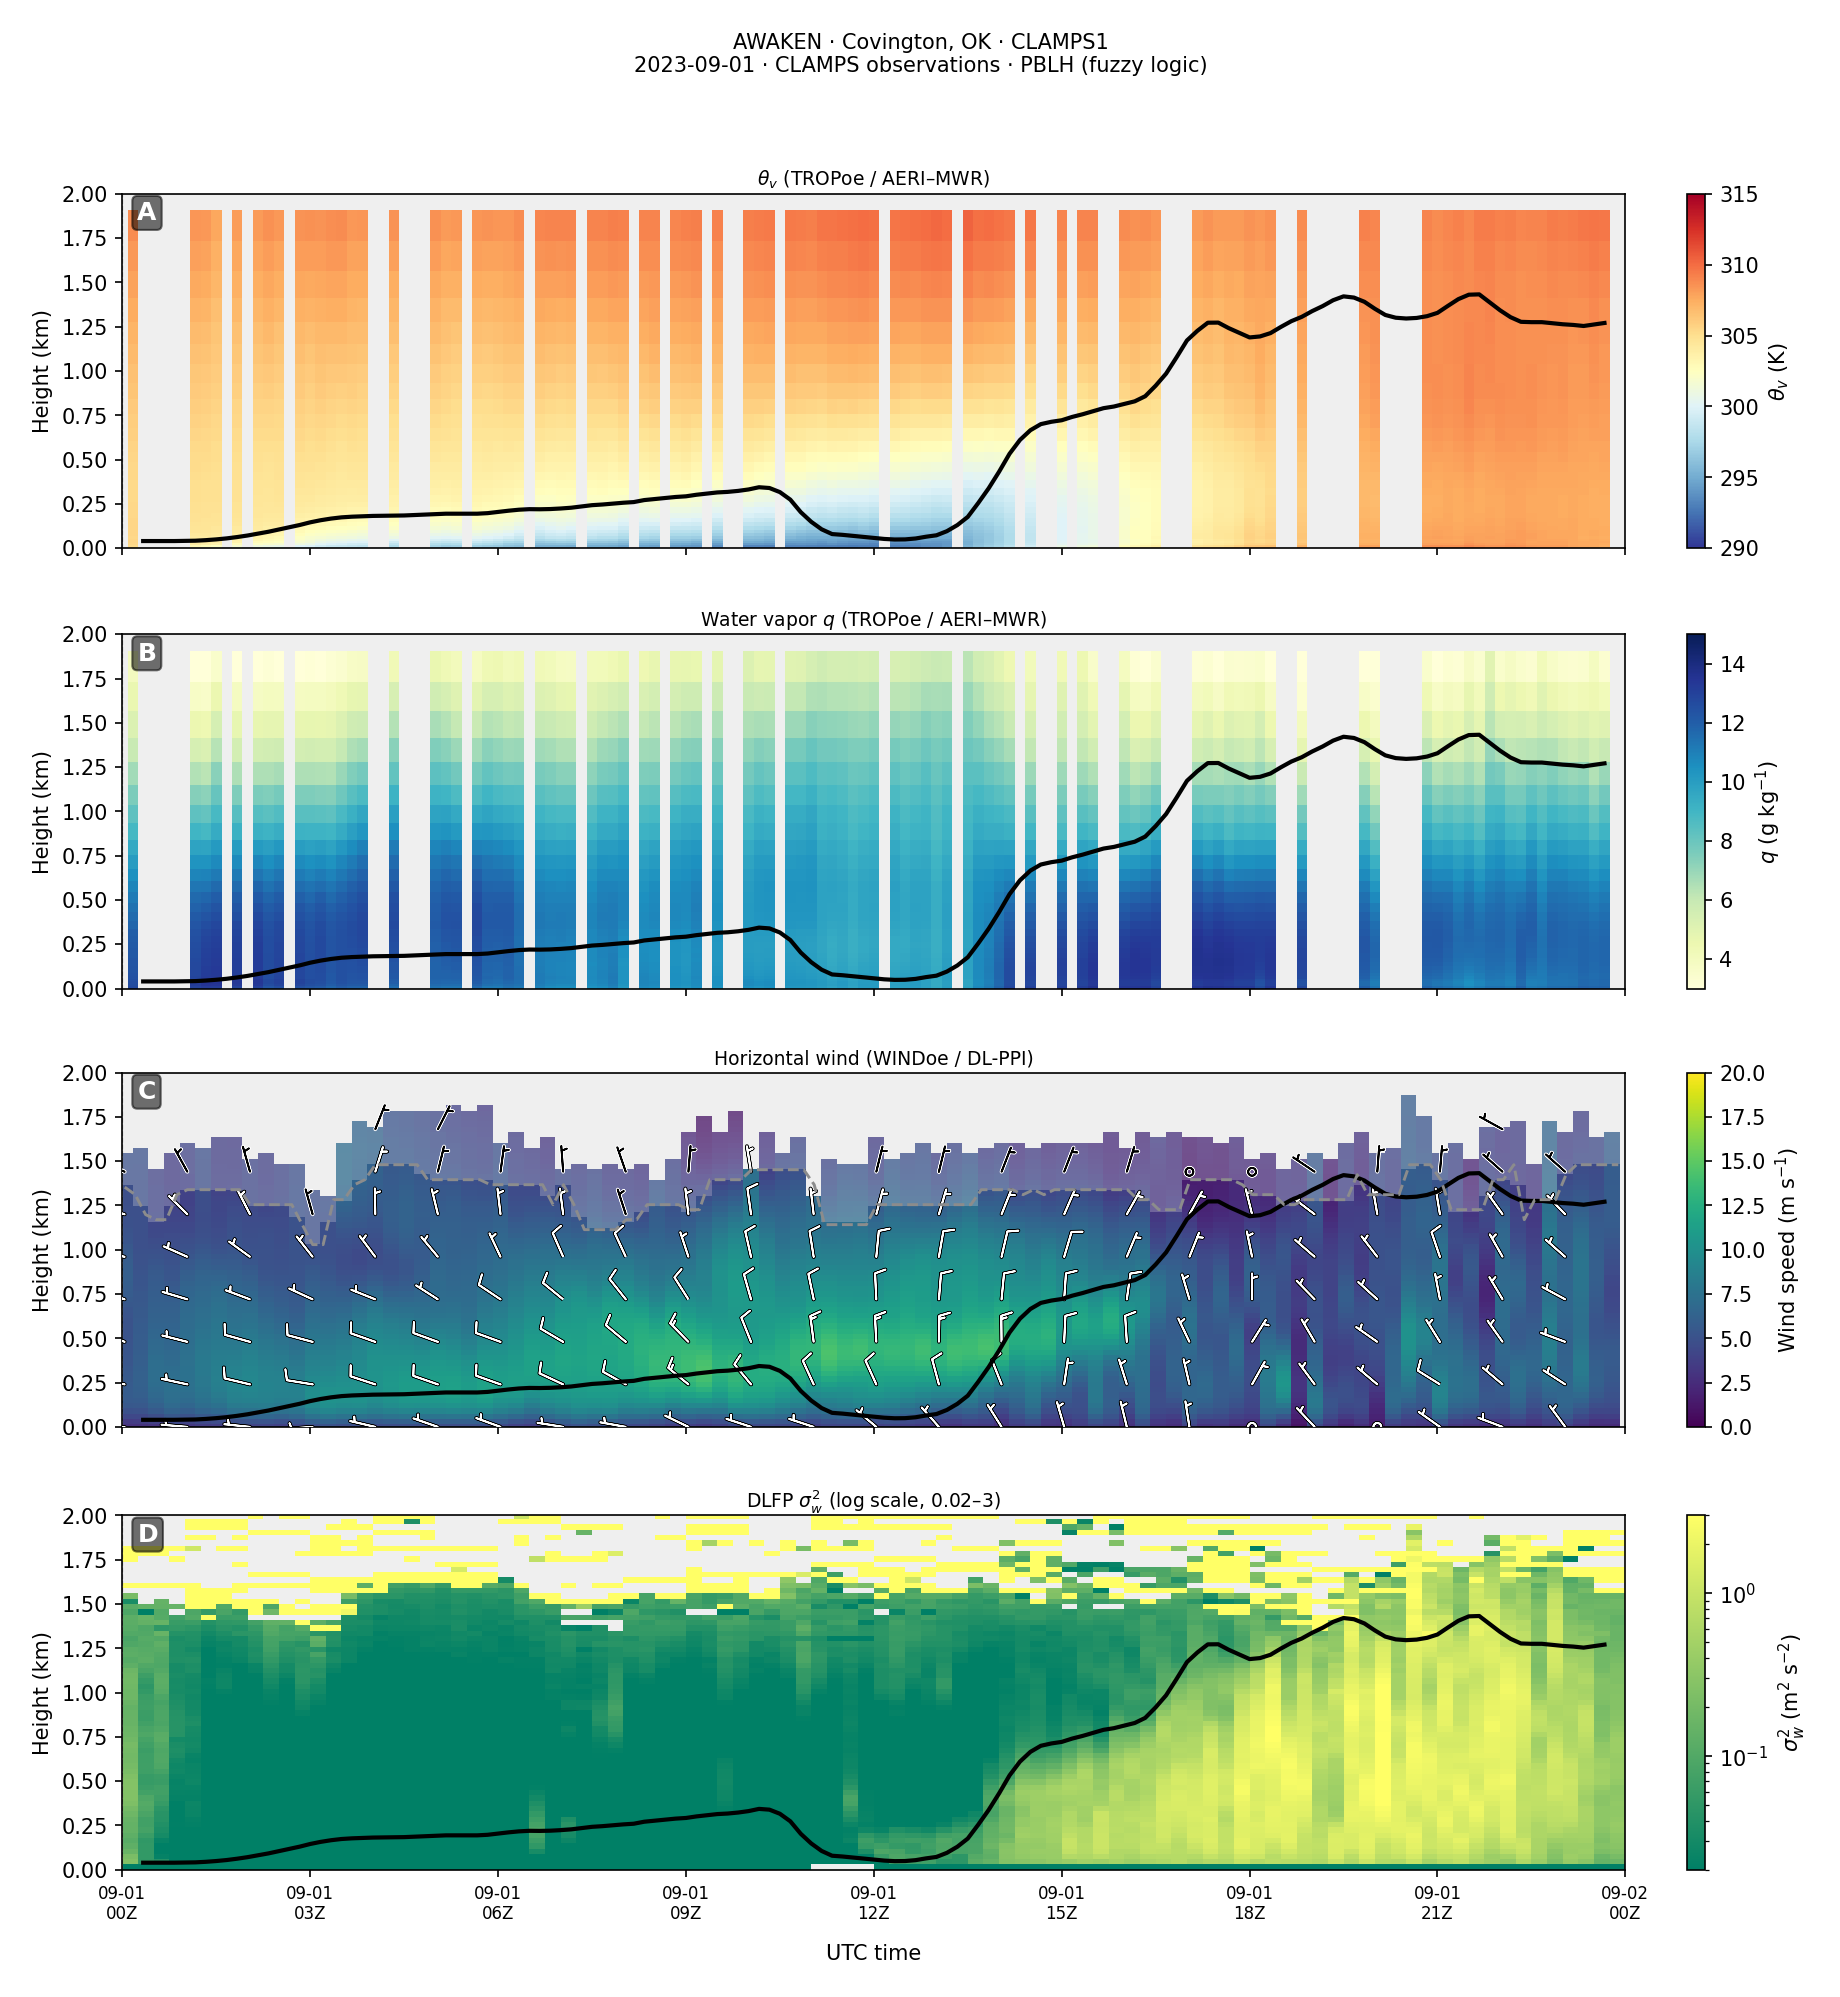
\includegraphics[width=\textwidth]{../../images/la_interaction_c1_instrument_template_4panel.png}
  \caption{Standard CLAMPS observations.}
  \label{fig:la_interaction_c1:la_interaction_c1_instrument_template_4panel}
\end{figure}
\subsection*{Case overview}
This case provides a comprehensive dataset for exploring land-atmosphere (L-A) interactions, demonstrating how surface energy partition controls the thermodynamic state and diurnal growth of the planetary boundary layer. CLAMPS1 did not operate a surface flux tower for this deployment; land-surface turbulent fluxes ($H$, $LE$), Obukhov length ($L$), and surface thermodynamics used in the coupling diagnostics come from the ARM Southern Great Plains Site A1 (S4) Energy Balance Bowen-Ratio system (ECOR, sgpecorsfS4.b1) at the AWAKEN supersite near Covington, Oklahoma, within the CLAMPS1 observation footprint. The first half of the period features a strongly stratified, stable nocturnal boundary layer. Following sunrise (\textasciitilde{}12:00 UTC), a rapid accumulation of surface sensible heat flux drives a violent flip in local stability regimes. This thermodynamic forcing triggers a clean, rapid expansion of the convective boundary layer (CBL), with the boundary layer height ($z_i$) climbing from near-surface levels to over 1.25 km in less than six hours.

\subsection*{Highlights}
\begin{itemize}
  \item Thermal Evolution \& Rapid Morning Erosion (Panel A): A strong surface-based stable layer is highly evident overnight in panel A of \hyperref[fig:la_interaction_c1:la_interaction_c1_instrument_template_4panel]{Standard CLAMPS observations}, featuring cold virtual potential temperatures ($\theta_v < 300\text{ K}$, deep blue shading) pinned below 250 m. Solar heating completely obliterates this inversion after 13:00 UTC, leading to a vertically uniform mixed layer ($\theta_v \approx 310\text{ K}$) that supports a steadily climbing fuzzy-logic PBLH peaking near 1.4 km at 21:00 UTC.
  \item Moisture Mixing, Dilution, \& LCL Divergence (Panel B): High specific humidity ($q \approx 11\text{ to }13\text{ g kg}^{-1}$) remains trapped in the shallow nocturnal layer before 12:00 UTC in panel B of \hyperref[fig:la_interaction_c1:la_interaction_c1_instrument_template_4panel]{Standard CLAMPS observations}. The diagnostic timeline in \hyperref[fig:la_interaction_c1:la_interaction_c1_aux_lcl_pblh_timeseries]{Surface LCL vs CLAMPS $z_i$} shows that this trapped low-level moisture causes the surface Lifting Condensation Level (LCL, blue line) to plunge overnight, nearly coupling with the shallow stable boundary layer ($z_i$, black line) around 10:00 UTC. In the afternoon, as the CBL deepens, dry air entrainment aloft drives an immense moisture deficit, causing the surface LCL to skyrocket past 2.0 km, leaving the 1.4 km boundary layer completely clear of land-coupled convective clouds.
  \item Surface Energy Partitioning \& Stability Overturning: The fundamental land-surface driver behind this rapid growth is detailed by the dual-panel flux metrics in \hyperref[fig:la_interaction_c1:la_interaction_c1_la_coupling_pblh_cumh_stability]{Cumulative surface fluxes vs $z_i$ and stability regimes}, which combine CLAMPS fuzzy-logic $z_i$ with ARM Site A1 (S4) ECOR cumulative fluxes. Panel A reveals an environment heavily dominated by sensible heat forcing, where accumulated sensible heat flux ($\int |H|dt$, red line) dramatically outpaces accumulated latent heat flux ($\int |LE|dt$, blue line). This lopsided partitioning forces a violent, instantaneous morning flip in the Obukhov stability parameter ($-h/L$, Panel B) from a highly stratified nocturnal stable regime ($<-10$, blue shading) straight into a heavily buoyancy-driven convective regime ($>10$, red shading) immediately following 13:00 UTC.
  \item Decoupled Low-Level Flow \& Turbulence Feedback (Panels C \& D): The kinematic profiles in panel C of \hyperref[fig:la_interaction_c1:la_interaction_c1_instrument_template_4panel]{Standard CLAMPS observations} capture a modest southerly nocturnal wind maximum ($10\text{ to }12\text{ m s}^{-1}$) around 0.5 km between 06:00 and 10:00 UTC. As the stability parameter flips, the explosive onset of the L-A feedback loop is mapped by the Doppler Lidar vertical velocity variance ($\sigma_w^2$, panel D). At 13:30 UTC, a sudden vertical plume of high variance ($1\text{ to }10\text{ m}^2\text{ s}^{-2}$, bright yellow/green shading) erupts, signaling intense vertical mixing that efficiently uniformizes horizontal momentum and slows down lower column wind speeds to $<5\text{ m s}^{-1}$.
\end{itemize}
\begin{figure}[htbp]
  \centering
  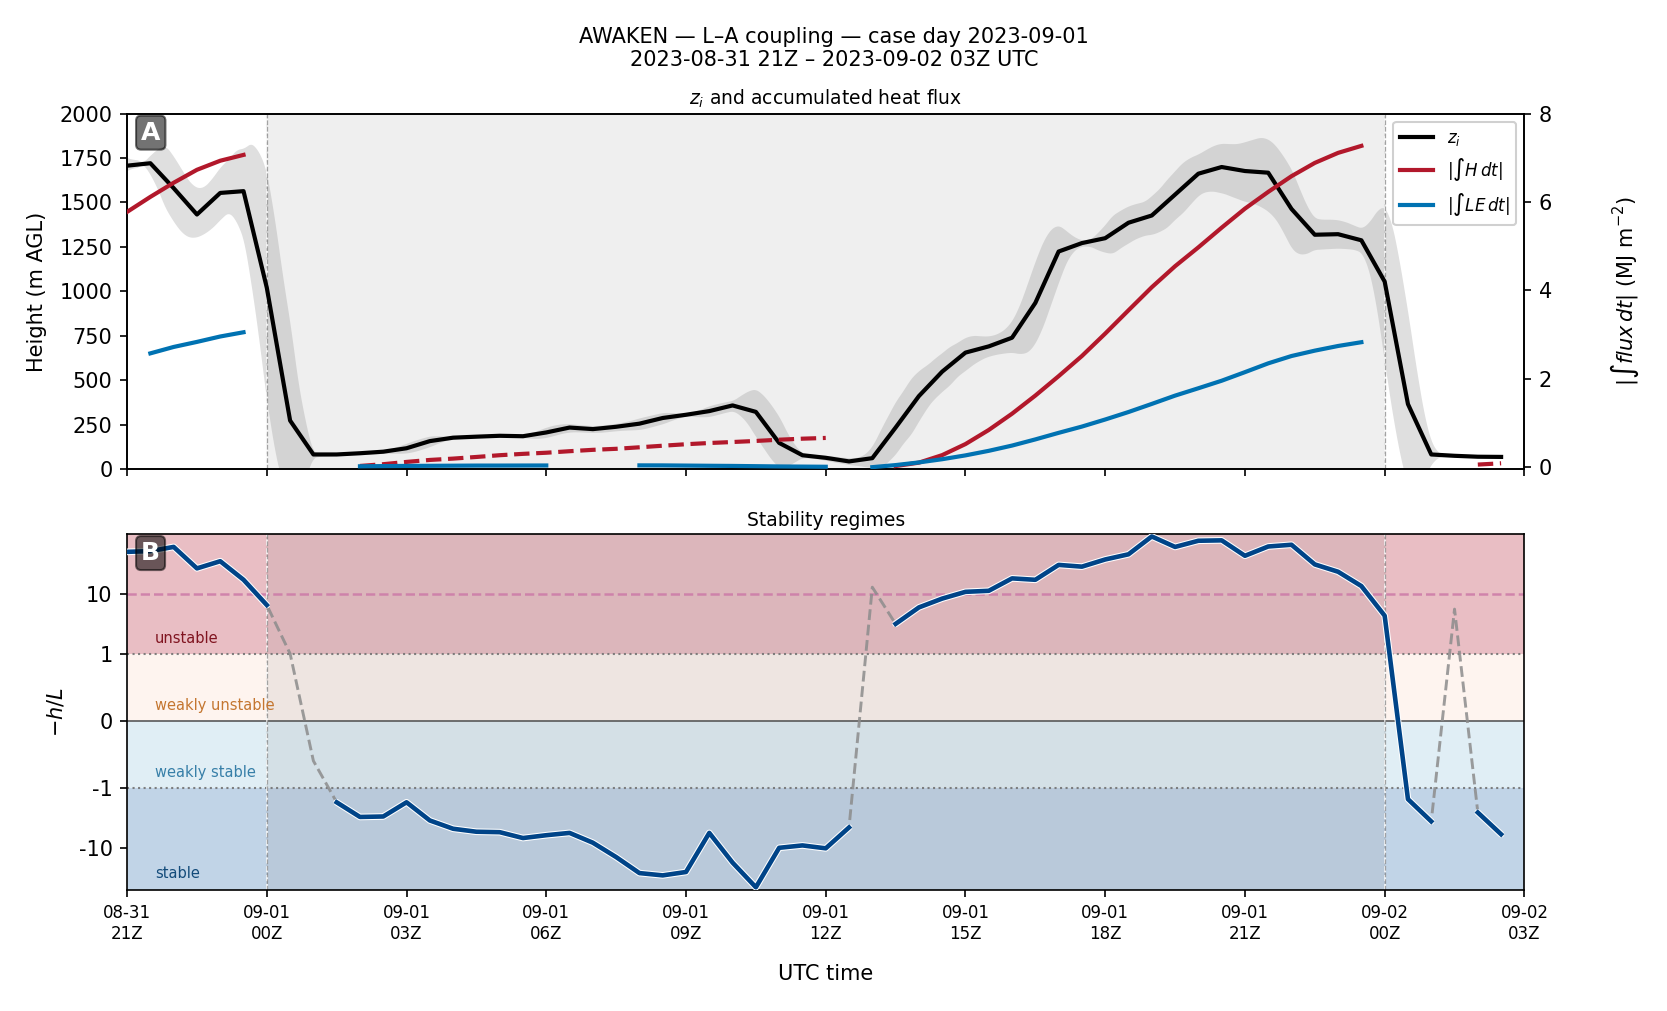
\includegraphics[width=0.92\textwidth]{../../images/la_interaction_c1_la_coupling_pblh_cumH_stability.png}
  \caption{Cumulative surface fluxes vs $z_i$ and stability regimes.
  Cumulative surface sensible ($\int |H|\,dt$) and latent ($\int |LE|\,dt$) heat fluxes from the ARM Southern Great Plains Site A1 (S4) Energy Balance Bowen-Ratio system (ECOR, sgpecorsfS4.b1) at the AWAKEN supersite near Covington, Oklahoma, shown alongside Obukhov stability ($-h/L$) regimes that drive the morning transition from stable to convective conditions.}
  \label{fig:la_interaction_c1:la_interaction_c1_la_coupling_pblh_cumh_stability}
\end{figure}
\begin{figure}[htbp]
  \centering
  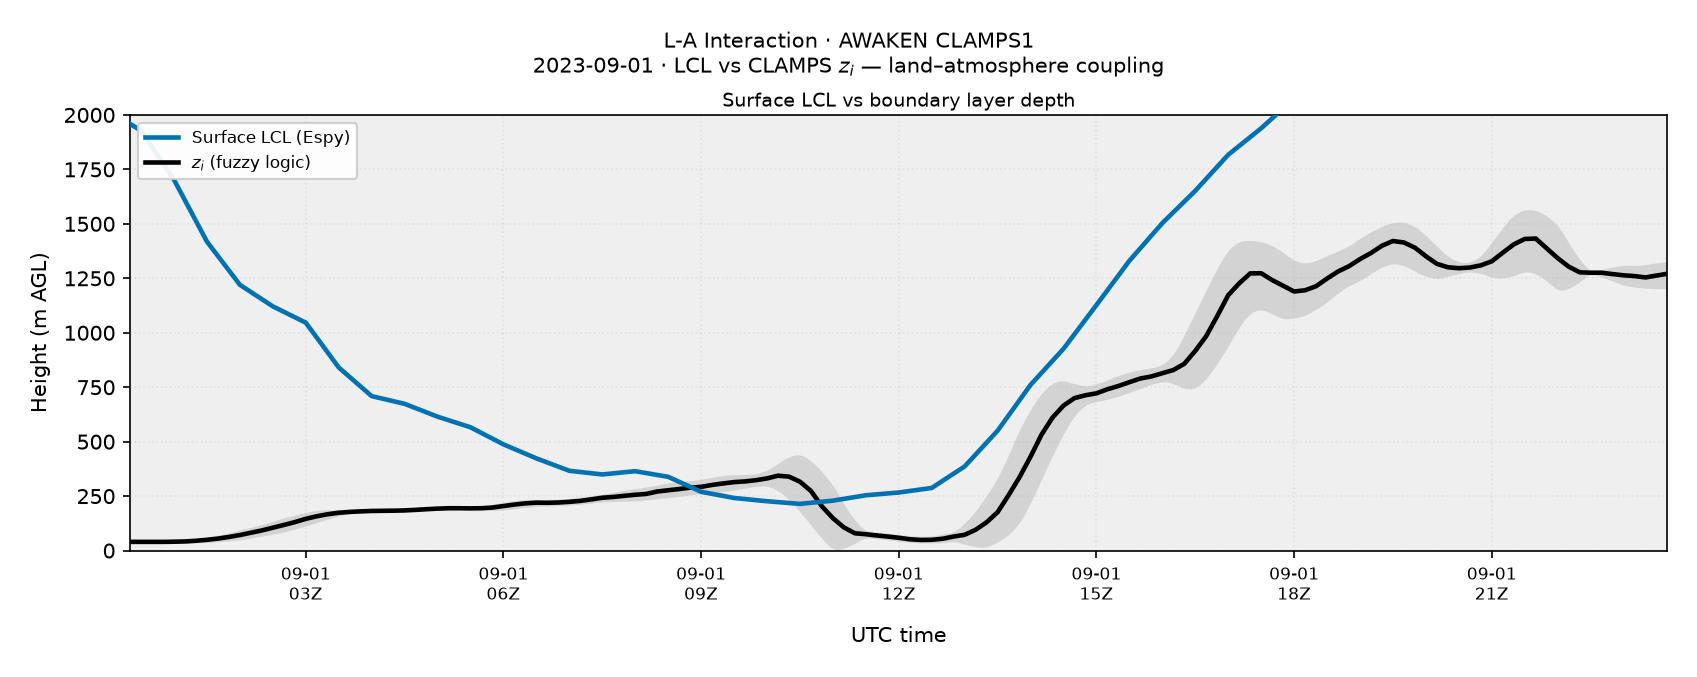
\includegraphics[width=0.92\textwidth]{../../images/la_interaction_c1_aux_lcl_pblh_timeseries.png}
  \caption{Surface LCL vs CLAMPS $z_i$.
  Surface lifting condensation level computed from ARM Site A1 (S4) ECOR air temperature and dewpoint (Espy approximation), compared with CLAMPS fuzzy-logic $z_i$, showing overnight LCL–$z_i$ coupling and afternoon divergence as dry entrainment deepens the CBL.}
  \label{fig:la_interaction_c1:la_interaction_c1_aux_lcl_pblh_timeseries}
\end{figure}
\section{Sharp Gradients}
\textit{CLAMPS2 $\cdot$ NWC Ops $\cdot$ Norman, OK $\cdot$ March 14, 2026 $\cdot$ fronts, gradients, boundaries, stable}

\begin{figure}[htbp]
  \centering
  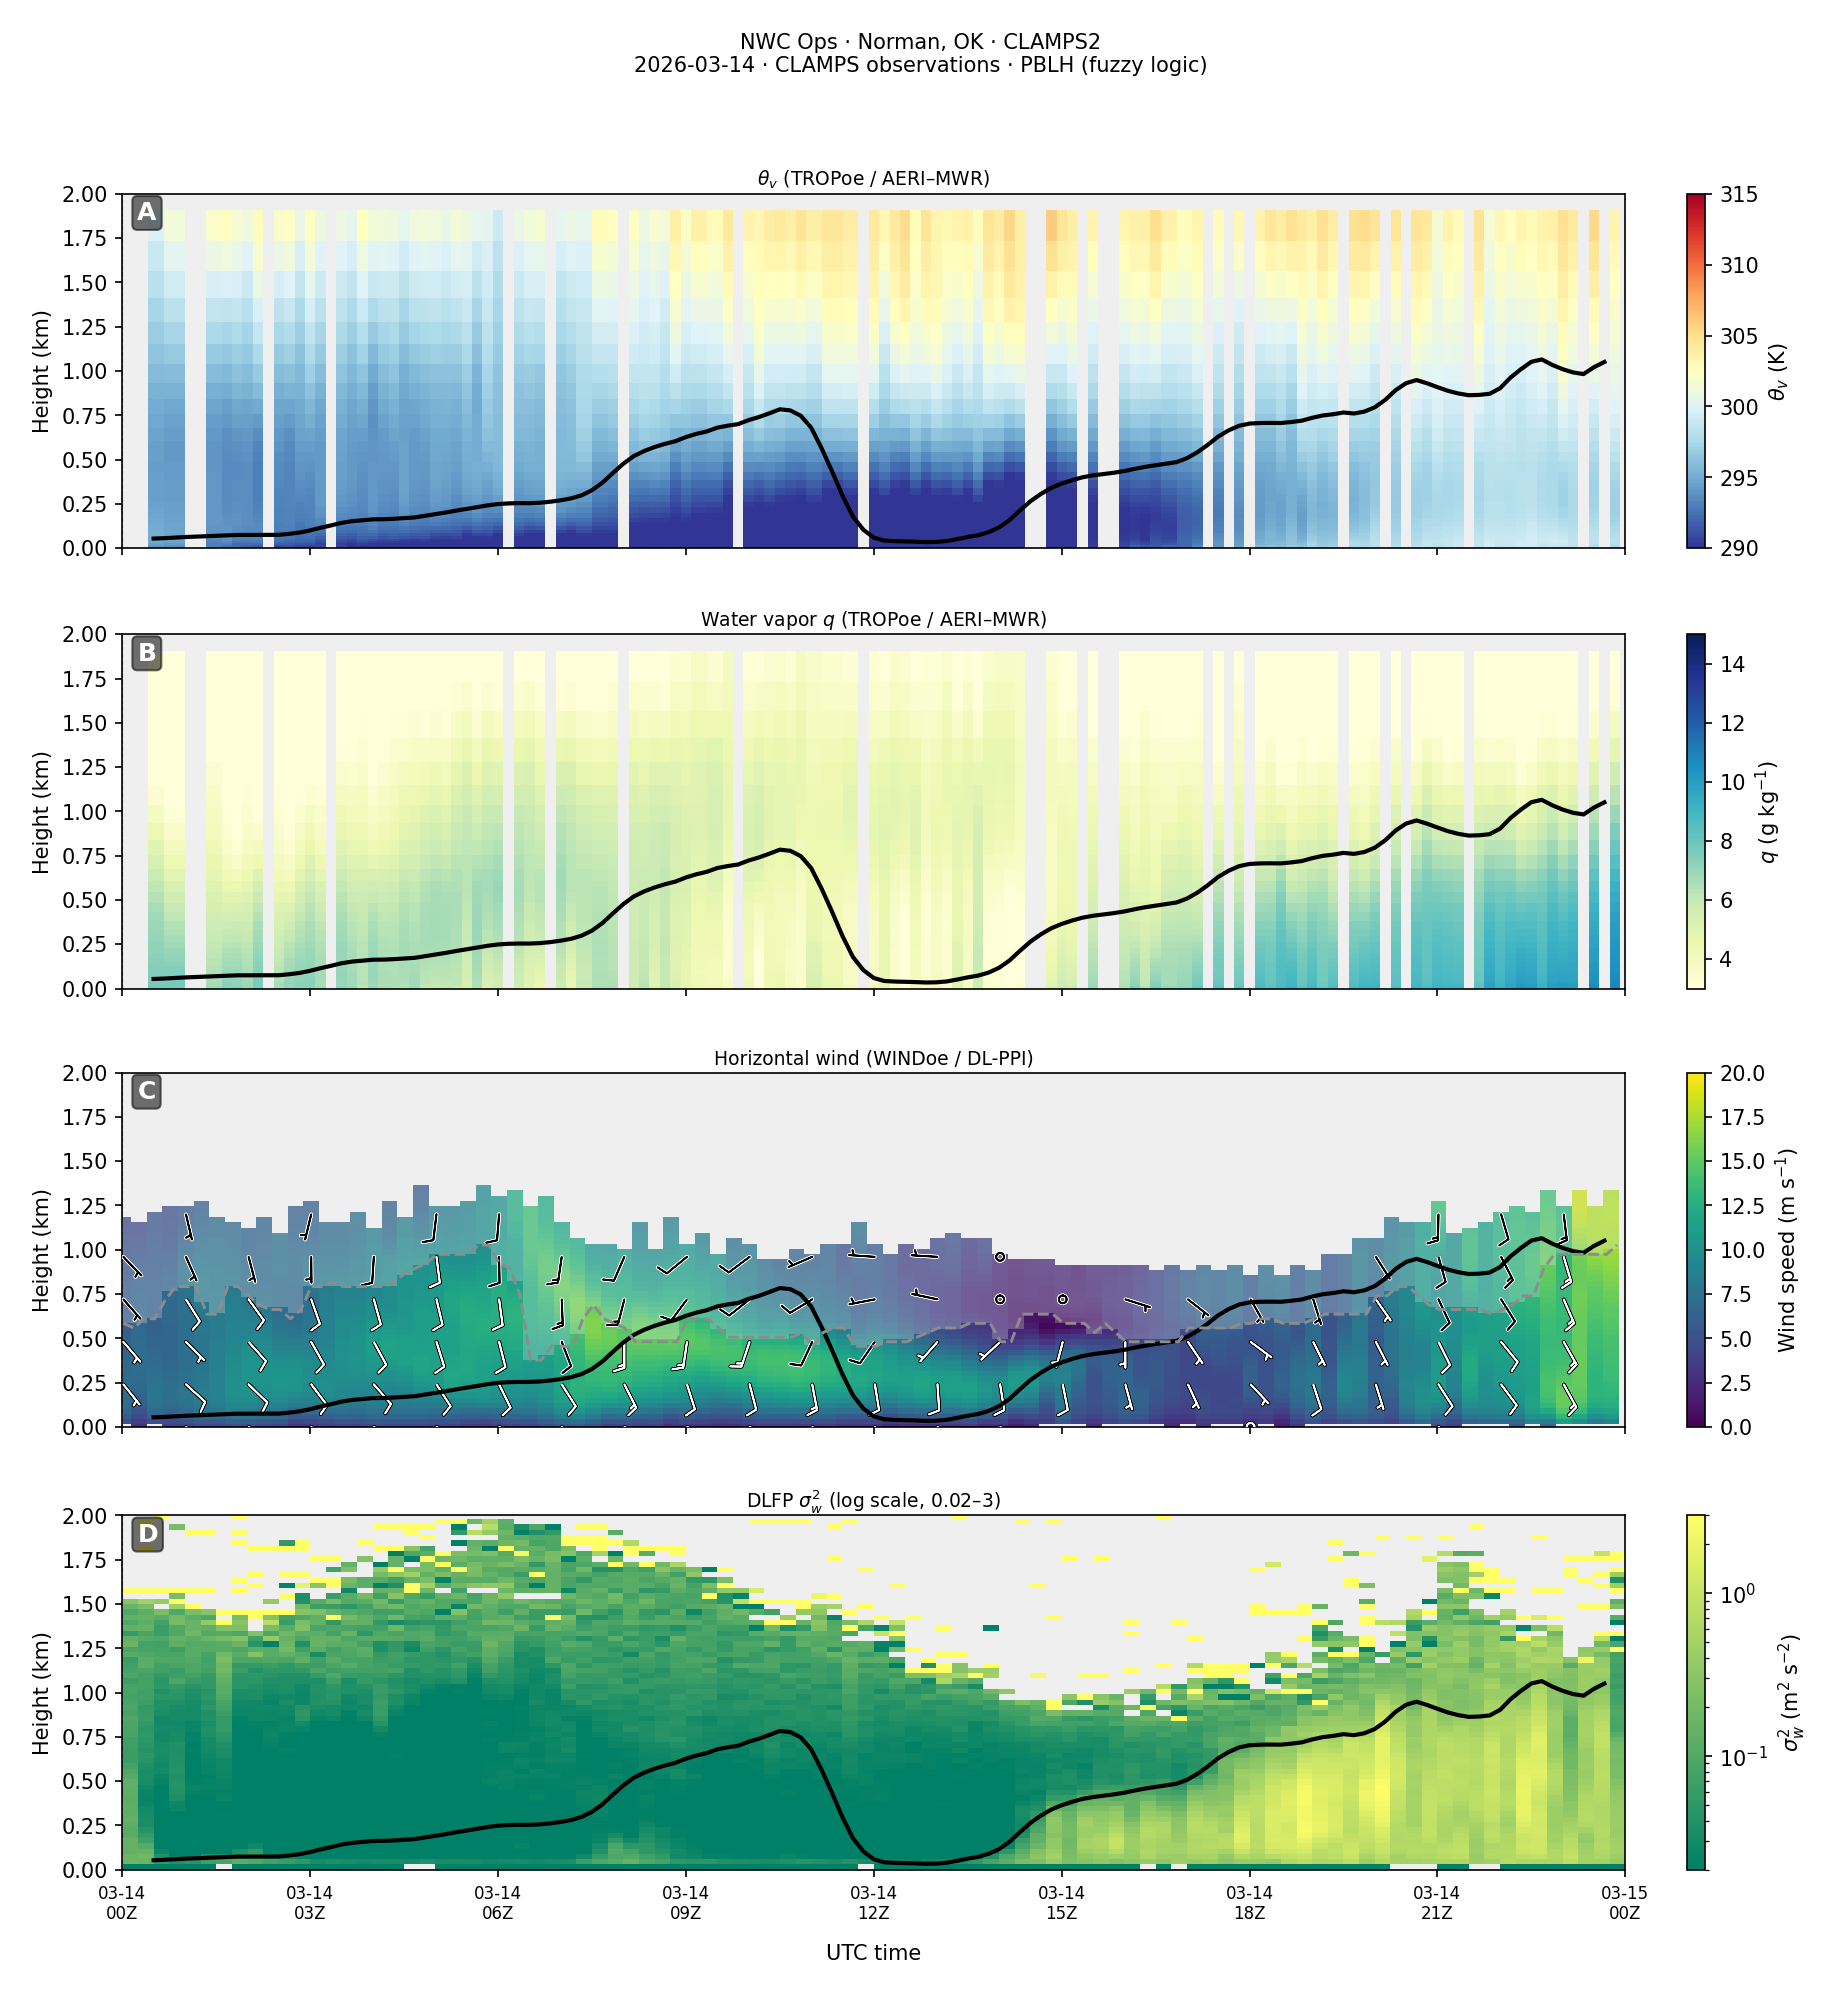
\includegraphics[width=\textwidth]{../../images/sharp_grad_c2_instrument_template_4panel.png}
  \caption{Standard CLAMPS observations.}
  \label{fig:sharp_grad_c2:sharp_grad_c2_instrument_template_4panel}
\end{figure}
\subsection*{Case overview}
This case study showcases the unique capability of the CLAMPS2 platform to capture the high-frequency evolution of sharp vertical ($\frac{\partial}{\partial z}$) and temporal ($\frac{\partial}{\partial t}$) gradients within a non-idealized stable boundary layer. Over a 24-hour window, a descending low-level wind maximum introduces vertical shear, triggering local dynamic instabilities that rapidly reshape lower-tropospheric features. By providing continuous, co-located thermodynamic and kinematic profiles, CLAMPS2 tracks how these gradients evolve in real time. The dataset exposes turbulent asymmetry where mechanically generated eddies continuously alter and weaken the vertical gradient of a passive scalar (moisture), while the vertical gradient of an active scalar (temperature) remains stratified due to surface radiative cooling. Later in the period, the platform records a rapid regime transition as horizontal advection again reorganizes the column's moisture profiles.

\subsection*{Highlights}
\begin{itemize}
  \item Descending jet and shear compression (Panel C): A core of high-momentum wind ($12\text{ to }15\text{ m s}^{-1}$) slopes downward over time in panel C of \hyperref[fig:sharp_grad_c2:sharp_grad_c2_instrument_template_4panel]{Standard CLAMPS observations}, compressing the vertical wind-shear gradient ($\frac{\partial U}{\partial z}$) directly against the stagnant surface air layer.
  \item Dynamic instability and mechanical turbulence ($Ri_b$ cross-section; Panel D): Between 04:00 and 08:00 UTC, as vertical wind shear intensifies, localized pockets within the lower kilometer drop below the critical threshold ($Ri_b < 0.25$, red contours) in \hyperref[fig:sharp_grad_c2:sharp_grad_c2_aux_rib_timeheight]{Bulk Richardson number $Ri_b$ (00–12 UTC)}, generating the nocturnal burst of vertical velocity variance ($\sigma_w^2$) resolved in panel D of \hyperref[fig:sharp_grad_c2:sharp_grad_c2_instrument_template_4panel]{Standard CLAMPS observations}.
  \item Moisture-gradient reversal (layer time series; $q$ time–height): Prior to 06:00 UTC, a standard moisture gradient is tracked in \hyperref[fig:sharp_grad_c2:sharp_grad_c2_aux_q_zi_timeseries]{Low- and mid-level $q$ vs $z_i$ (00–00 UTC)} with high moisture near the surface ($0\text{ to }250\text{ m}$, solid blue line) and drier air aloft ($750\text{ to }1000\text{ m}$, dot-dashed orange line). As shear-driven eddies peak, the two layers completely cross over time: near-surface $q$ drops from $7\text{ to }3.5\text{ g kg}^{-1}$ while the upper layer moistens. In the zoomed spatial domain of \hyperref[fig:sharp_grad_c2:sharp_grad_c2_aux_q_wind_timeheight]{$q$ time–height with wind barbs (03–18 UTC)}, wind-barb overlays resolve a sloped channel of low-level drying tied directly to this turbulent mixing window.
  \item Scalar asymmetry at 12:00 UTC (profile snapshots): One-dimensional profiles in \hyperref[fig:sharp_grad_c2:sharp_grad_c2_aux_scalar_asymmetry_profiles]{Scalar asymmetry — $\theta_v$ and $q$ (06, 09, 12, 18 UTC)} provide direct evidence that active and passive scalar gradients evolve along decoupled pathways under stable stratification. At 12:00 UTC (solid black line), virtual potential temperature ($\theta_v$) exhibits massive resistance to mechanical mixing—the surface thermal gradient ($\frac{\partial \theta_v}{\partial z}$) remains intensely sharp because buoyancy and continuous radiative cooling suppress vertical displacements. Conversely, the specific-humidity gradient is entirely hollowed out and inverted near the ground, where the passive scalar $q$ is easily redistributed into an isolated reservoir ($q \approx 5\text{ g kg}^{-1}$) trapped near $0.75\text{ km}$.
  \item Afternoon advection-dominated recovery ($q$ vs $z_i$ time series; Panel C): Following sunrise, CLAMPS2 documents a rapid transition from a shear-dominated regime to an advection-dominated regime. Standard boundary-layer theory predicts that as solar heating expands the planetary boundary layer height $z_i$ (dashed black line in \hyperref[fig:sharp_grad_c2:sharp_grad_c2_aux_q_zi_timeseries]{Low- and mid-level $q$ vs $z_i$ (00–00 UTC)}), entrainment of dry free-tropospheric air should dilute column moisture. Instead, low- and mid-level moisture surge upward in tandem after 14:00 UTC, with surface specific humidity climbing past $10\text{ g kg}^{-1}$. Panel C of \hyperref[fig:sharp_grad_c2:sharp_grad_c2_instrument_template_4panel]{Standard CLAMPS observations} confirms the underlying physical mechanism: the lowest $500\text{ m}$ reorganizes into a highly efficient southerly conveyor belt, loading the boundary layer with Gulf moisture faster than convective entrainment can dry it.
\end{itemize}
\begin{figure}[htbp]
  \centering
  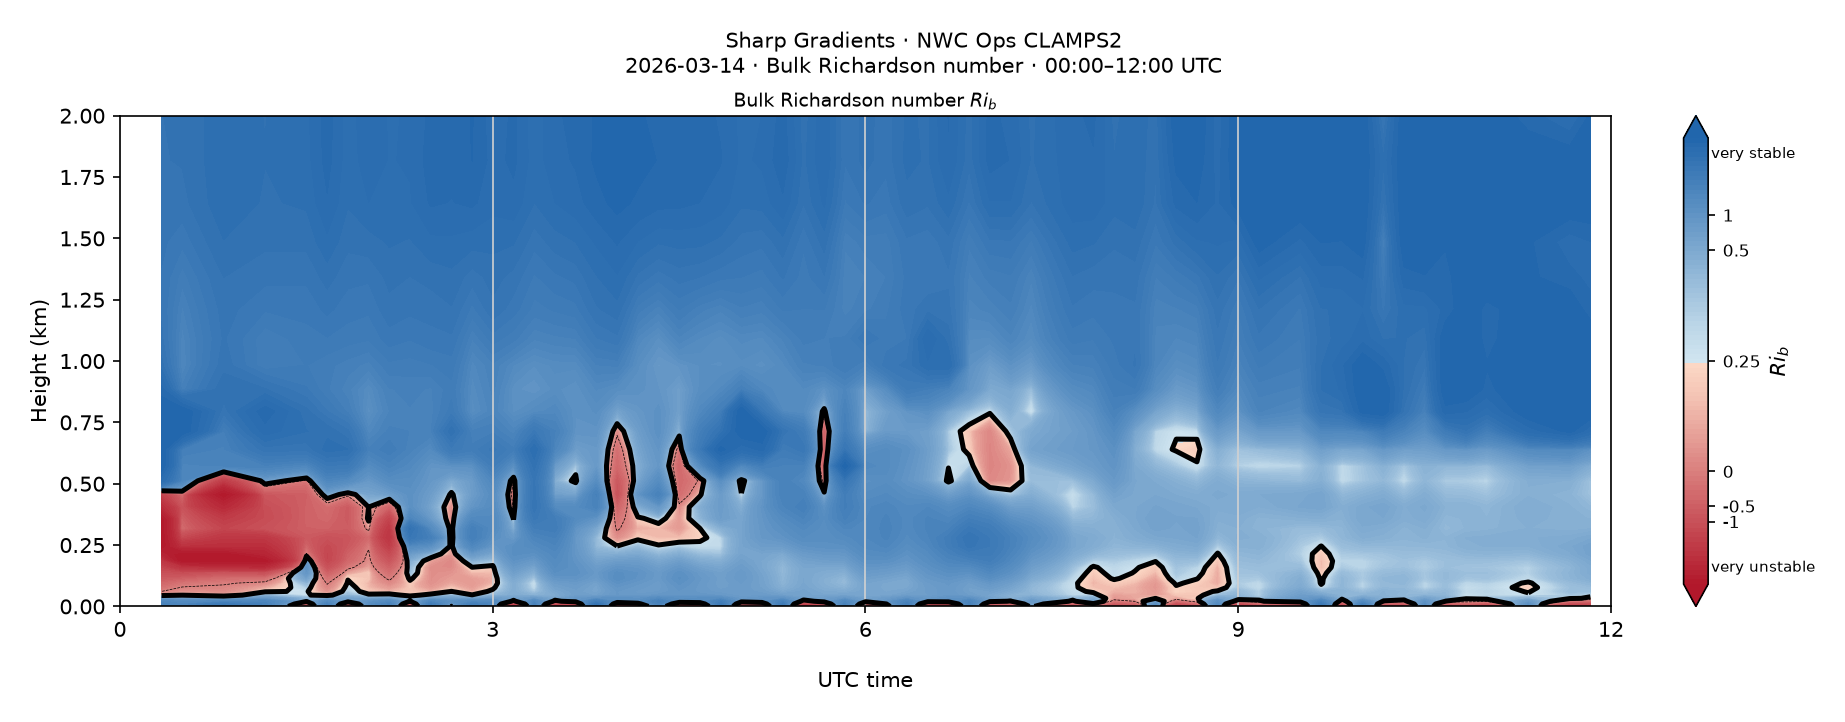
\includegraphics[width=0.92\textwidth]{../../images/sharp_grad_c2_aux_rib_timeheight.png}
  \caption{Bulk Richardson number $Ri_b$ (00–12 UTC).
  Bulk Richardson number $Ri_b$ (00–12 UTC) mapping mechanically generated turbulence pockets ($Ri_b < 0.25$) beneath the descending nocturnal wind maximum.}
  \label{fig:sharp_grad_c2:sharp_grad_c2_aux_rib_timeheight}
\end{figure}
\begin{figure}[htbp]
  \centering
  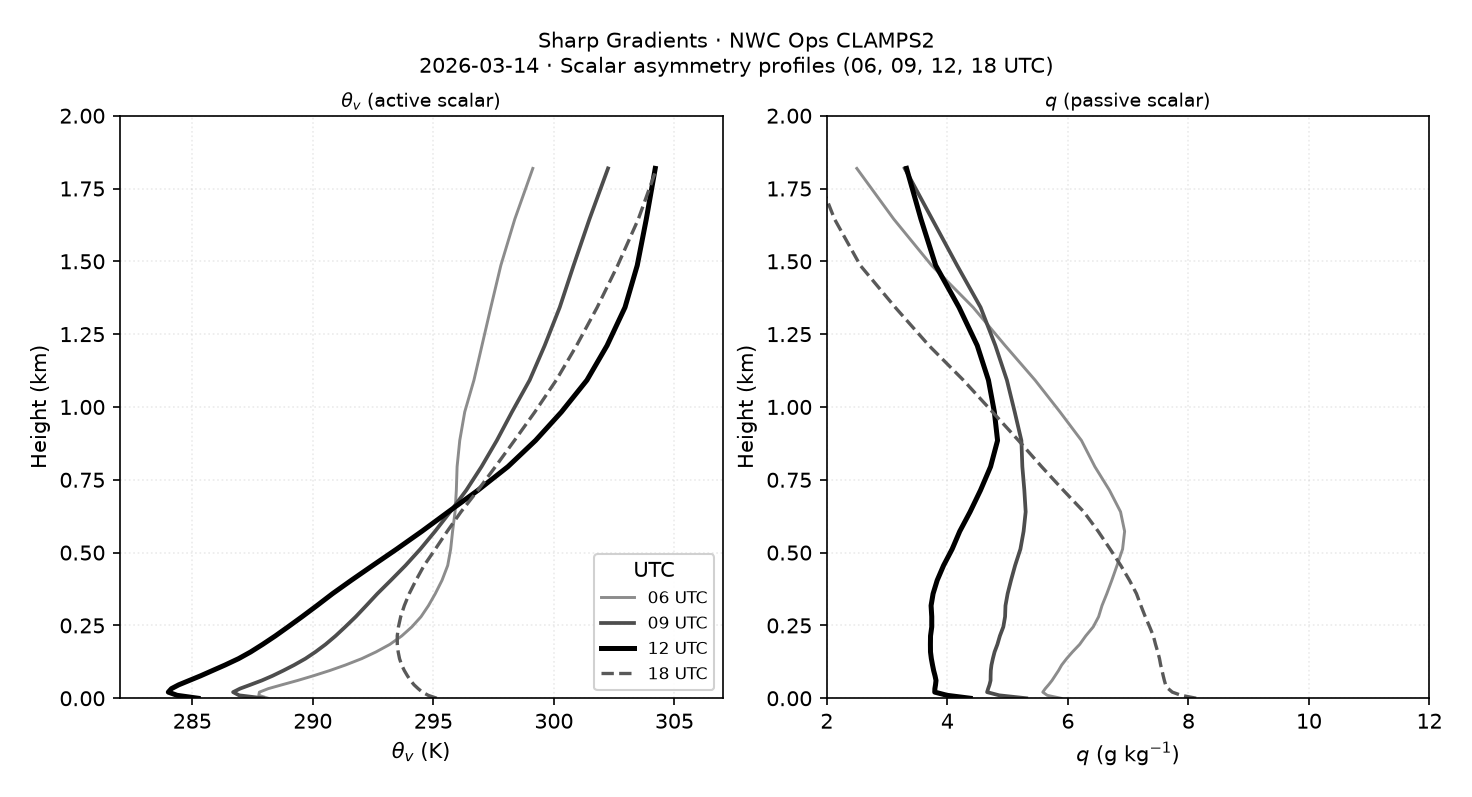
\includegraphics[width=0.92\textwidth]{../../images/sharp_grad_c2_aux_scalar_asymmetry_profiles.png}
  \caption{Scalar asymmetry — $\theta_v$ and $q$ (06, 09, 12, 18 UTC).
  $\theta_v$ and $q$ profile snapshots at 06, 09, 12, and 18 UTC demonstrating asymmetric evolution of active (temperature) and passive (moisture) scalar gradients under stable stratification.}
  \label{fig:sharp_grad_c2:sharp_grad_c2_aux_scalar_asymmetry_profiles}
\end{figure}
\begin{figure}[htbp]
  \centering
  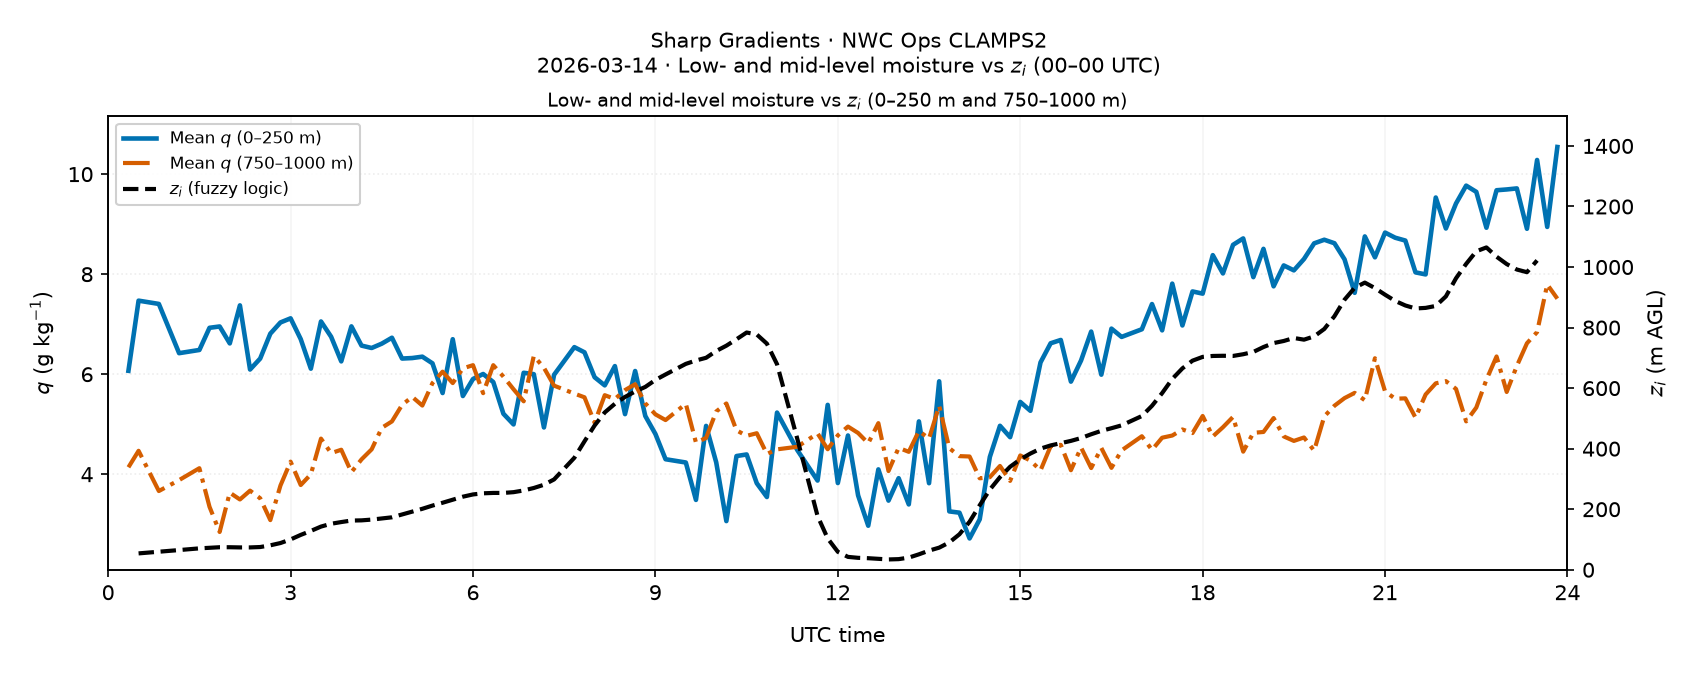
\includegraphics[width=0.92\textwidth]{../../images/sharp_grad_c2_aux_q_zi_timeseries.png}
  \caption{Low- and mid-level $q$ vs $z_i$ (00–00 UTC).
  Near-surface ($0$–$250$ m) and mid-level ($750$–$1000$ m) specific humidity tracked against $z_i$, capturing the moisture-gradient reversal during shear-driven turbulent mixing.}
  \label{fig:sharp_grad_c2:sharp_grad_c2_aux_q_zi_timeseries}
\end{figure}
\begin{figure}[htbp]
  \centering
  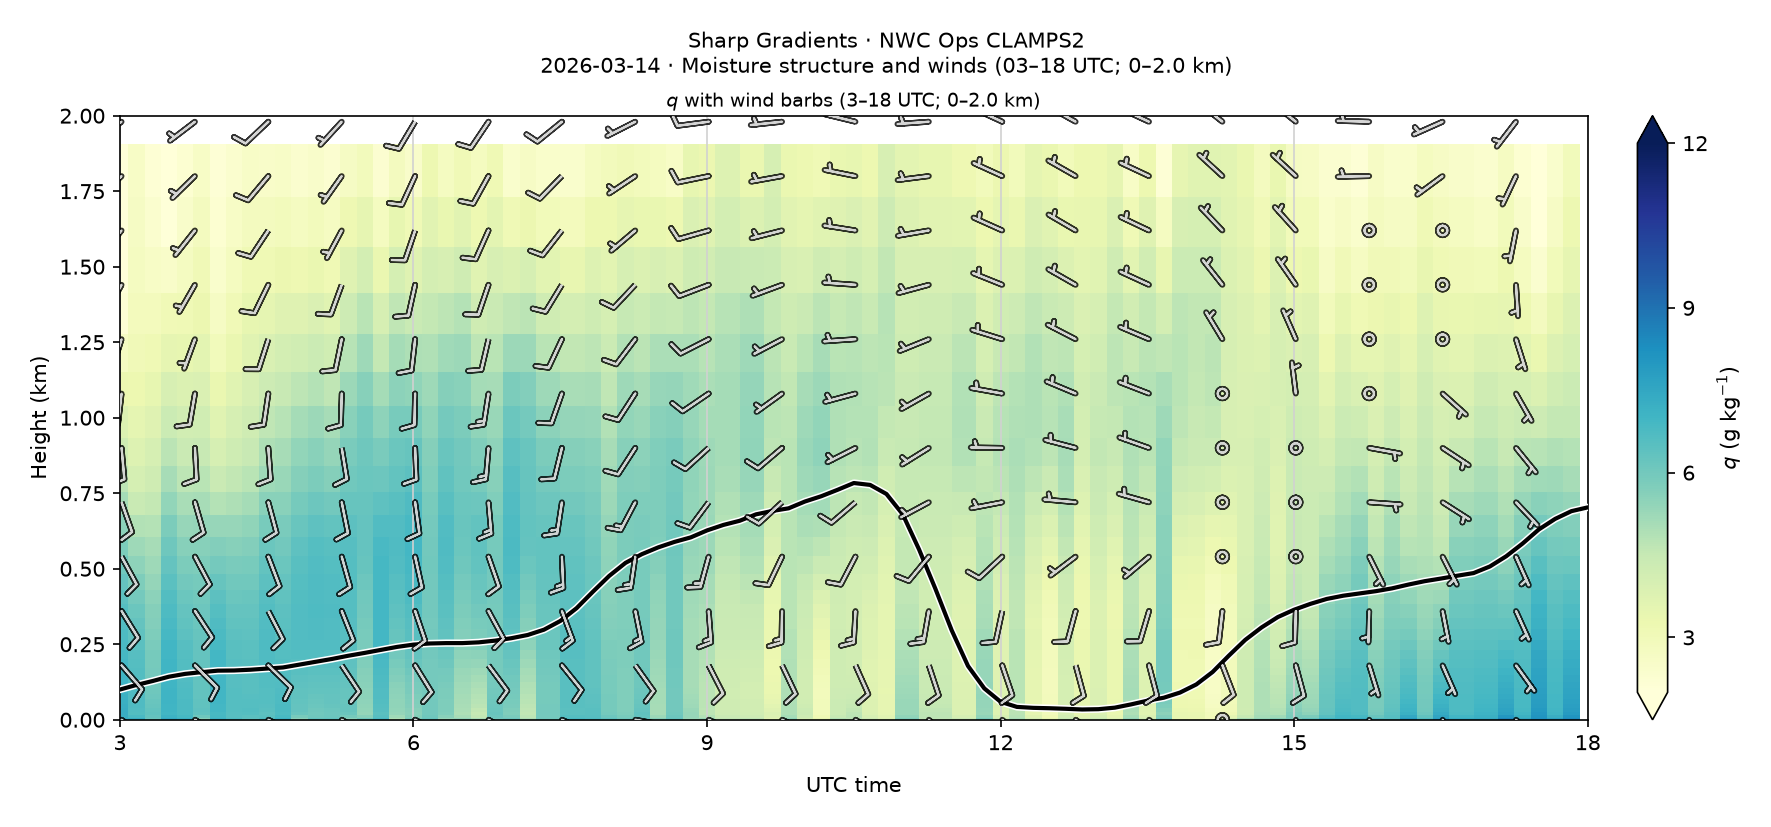
\includegraphics[width=0.92\textwidth]{../../images/sharp_grad_c2_aux_q_wind_timeheight.png}
  \caption{$q$ time–height with wind barbs (03–18 UTC).
  Zoomed $q$ time–height (03–18 UTC) with wind-barb overlay resolving the sloped channel of low-level drying tied to the nocturnal mixing window.}
  \label{fig:sharp_grad_c2:sharp_grad_c2_aux_q_wind_timeheight}
\end{figure}
\section{Strong Synoptic Cold Front}
\textit{CLAMPS2 $\cdot$ NWC Ops $\cdot$ Norman, OK $\cdot$ March 27, 2026 $\cdot$ fronts, boundaries, stable}

\begin{figure}[htbp]
  \centering
  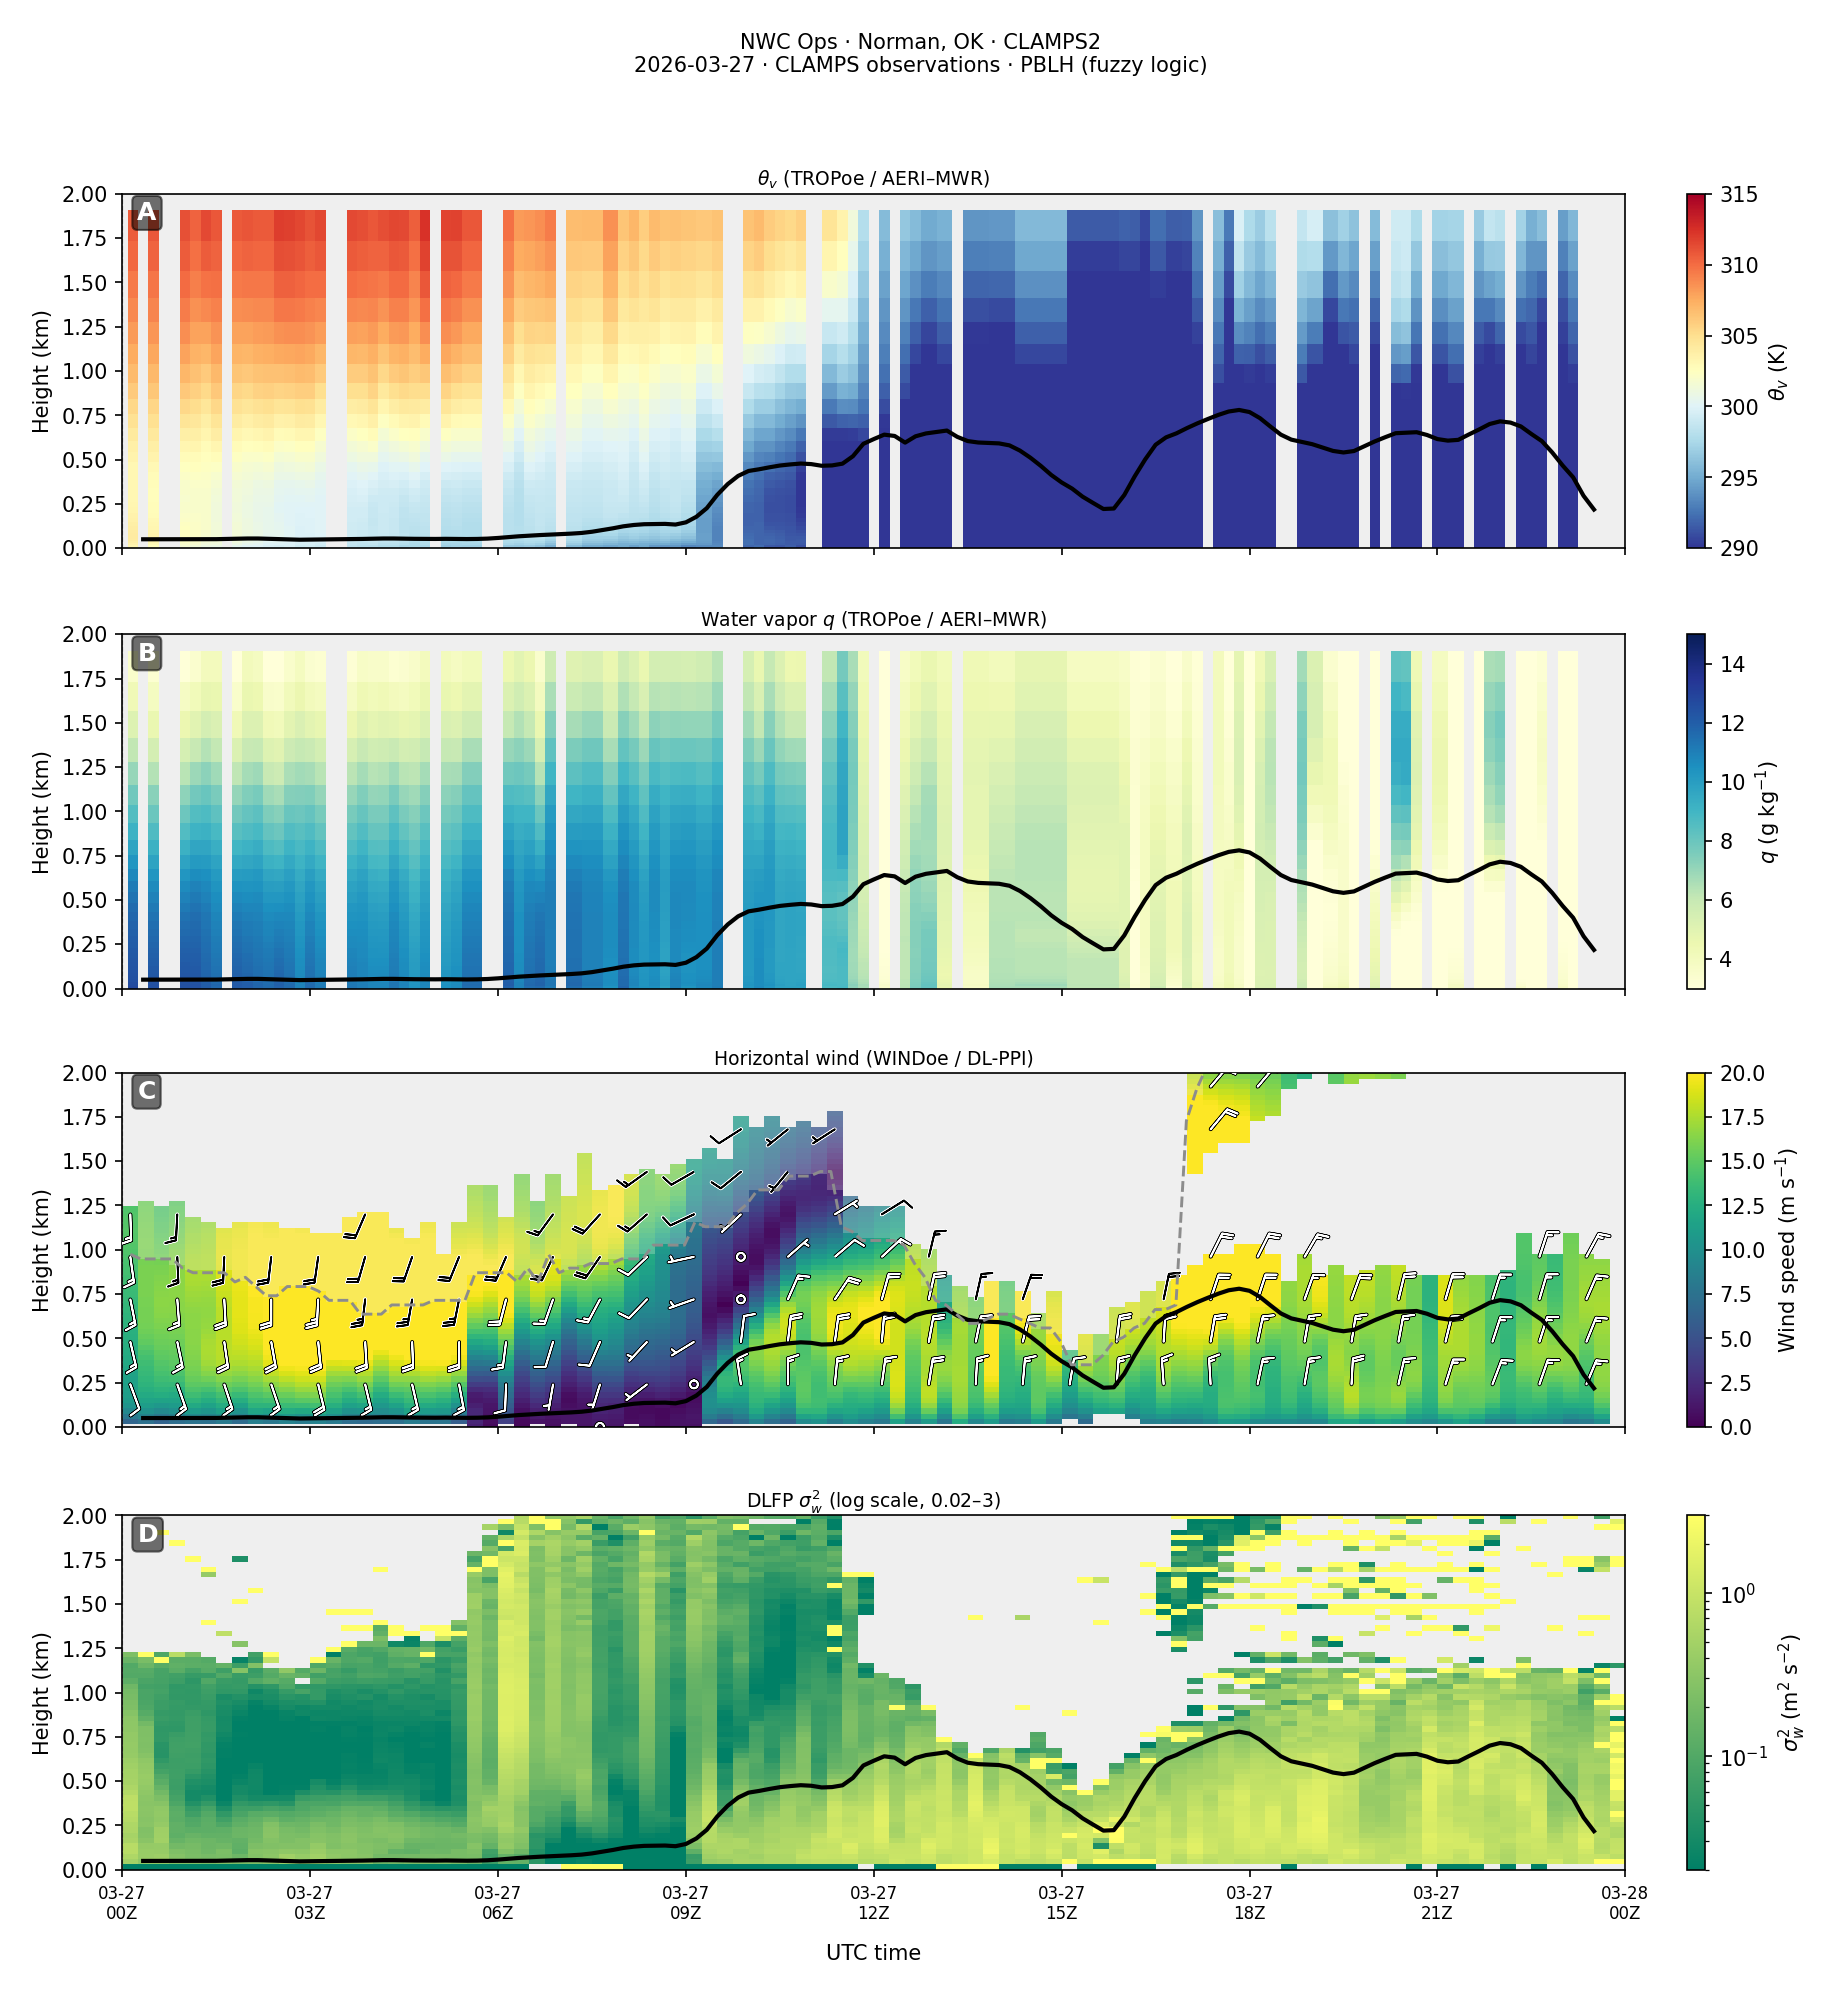
\includegraphics[width=\textwidth]{../../images/fropa_c2_instrument_template_4panel.png}
  \caption{Standard CLAMPS observations.}
  \label{fig:fropa_c2:fropa_c2_instrument_template_4panel}
\end{figure}
\subsection*{Case overview}
This case captures a high-amplitude, classic synoptic cold front crosscutting the CLAMPS2 platform in Norman, Oklahoma, providing a textbook demonstration of a counterintuitive nocturnal warming event (Nallapareddy et al. 2011; doi: 10.1175/JAMC-D-11-020.1). Prior to the front approaching (e.g., 06:00 UTC), the lower troposphere is stratified with a surface-based nocturnal radiation inversion below a high-momentum warm sector. At 09:00 UTC, the surface cold front arrives. Rather than driving an immediate temperature drop, the winds associated with the frontal head mechanically mix out the shallow radiation inversion. This turbulent mixing brings warmer air from the residual layer aloft down to the surface, forcing a transient temperature spike. Following this mixing episode, the advancing dense polar air mass fully undercuts the column, initiating a decline in both temperature and moisture. CLAMPS2's surface met station was not operating for this case; the surface meteogram uses Oklahoma Mesonet station NRMN (Norman), located a few miles north of the profiler site.

\subsection*{Highlights}
\begin{itemize}
  \item Norman Mesonet Surface Signature: With no CLAMPS surface meteorological data for this deployment, the independent Oklahoma Mesonet station at Norman (NRMN) compiled in \hyperref[fig:fropa_c2:fropa_c2_aux_surface_meteogram]{Norman Mesonet surface meteogram (06–15 UTC)} documents the crisp surface footprint of the frontal passage. The instruments record a hydrostatic pressure jump (from $\sim$971.5 hPa to $\sim$973 hPa) beginning at 09:00 UTC. Rather than an immediate temperature crash, the surface temperature actually rises for a brief period after 09:00 UTC as the frontal head mechanically mixes out the shallow nocturnal inversion. This is followed by a rapid thermal decline as the dense polar air mass undercuts the column. The wind vector shifts cleanly from pre-frontal southerlies to intense north-northwesterly flow exceeding $10\text{ m s}^{-1}$.
  \item Thermodynamic Column Structure \& Frontal Slope (Panel A): The column in \hyperref[fig:fropa_c2:fropa_c2_instrument_template_4panel]{Standard CLAMPS observations} exhibits a deep, uniform warm layer ($\theta_v > 305\text{ K}$) prior to the front. At 09:00 UTC, the cold air mass undercuts the warm sector, with the boundary sloping upward and backward over time—reaching an altitude of 1.0 km by 13:00 UTC. Near-surface $\theta_v$ is temporarily elevated at the exact moment of passage due to the mixing event, before plummeting into the deep blue zone ($< 285\text{ K}$) as the cold pool settles. The automated retrieval flags (black dots) trace cloud bases forming directly along the sloped leading edge of the front between 11:00 and 14:00 UTC.
  \item Post-Frontal Moisture Decline (Panel B): The pre-frontal air mass carries moderate moisture ($q \approx 9\text{ to }11\text{ g kg}^{-1}$) in panel B of \hyperref[fig:fropa_c2:fropa_c2_instrument_template_4panel]{Standard CLAMPS observations}. As the front passes, the forced frontal ascent keeps moisture elevated up the slope. However, once the true core of the continental air mass arrives after 13:00 UTC, specific humidity undergoes a catastrophic collapse, flatlining below $4\text{ g kg}^{-1}$ (pale yellow shading) through the entire lower 1.5 km column.
  \item Kinematic Discontinuity \& Radar Verification (Panel C): The wind field in panel C of \hyperref[fig:fropa_c2:fropa_c2_instrument_template_4panel]{Standard CLAMPS observations} provides a flawless visual definition of a sharp synoptic front. Pre-frontal: intense southwesterly winds ($15\text{ to }20\text{ m s}^{-1}$) dominate. The interface: right at 09:00 UTC, a narrow, vertical channel of near-zero wind velocity (deep purple) marks the immediate frontal convergence zone. This precise timing is verified by the KTLX NEXRAD radar snapshot in \hyperref[fig:fropa_c2:fropa_c2_ktlx_88d_20230327_0900]{KTLX 88D reflectivity at 09:00 UTC}, which captures a distinct reflectivity fine-line and sharp radial velocity discontinuity boundary slicing directly over the Norman star indicator at 08:56 UTC. Post-frontal: winds instantly veer to the north-northwest, developing into an intense post-frontal wind maximum exceeding $20\text{ m s}^{-1}$ aloft that rides directly above the surface cold pool.
  \item Boundary-Layer Turbulence Across the Front (Panel D): The Doppler Lidar vertical velocity variance ($\sigma_w^2$, panel D of \hyperref[fig:fropa_c2:fropa_c2_instrument_template_4panel]{Standard CLAMPS observations}) transitions from a highly turbulent pre-frontal regime to a temporarily suppressed state directly beneath the dense post-frontal inversion. Turbulence is highly elevated at the exact moment of frontal passage as the mechanical head of the front violently mixes the shallow nocturnal inversion.
  \item Profile Snapshots at Frontal Passage (03, 06, 09:15, 12 UTC): Vertical profiles in \hyperref[fig:fropa_c2:fropa_c2_aux_front_theta_sigma_profiles]{$\theta_v$ and $\sigma_w^2$ profiles at 03, 06, 09:15, and 12 UTC} resolve the evolving coupling between $\theta_v$ and $\sigma_w^2$ in the lowest kilometer at four snapshots bracketing passage. At 03Z, a sharp surface inversion separates cool near-surface air from the warm residual layer aloft while turbulence remains modest. By 06Z the prefrontal transition is beginning. Horizontal winds are slowing and the mixing activity maintained through the night up to this point is collapsing. At 09:15Z, coincident with Mesonet-documented mixing and the transient surface warm spike, $\sigma_w^2$ intensifies and the near-surface $\theta_v$ profile temporarily homogenizes as residual-layer air is mixed downward. At 12Z, following undercutting by the dense cool air mass, $\theta_v$ collapses through the column while elevated $\sigma_w^2$ marks continued mechanical shear above the deepening cold pool.
\end{itemize}
\begin{figure}[htbp]
  \centering
  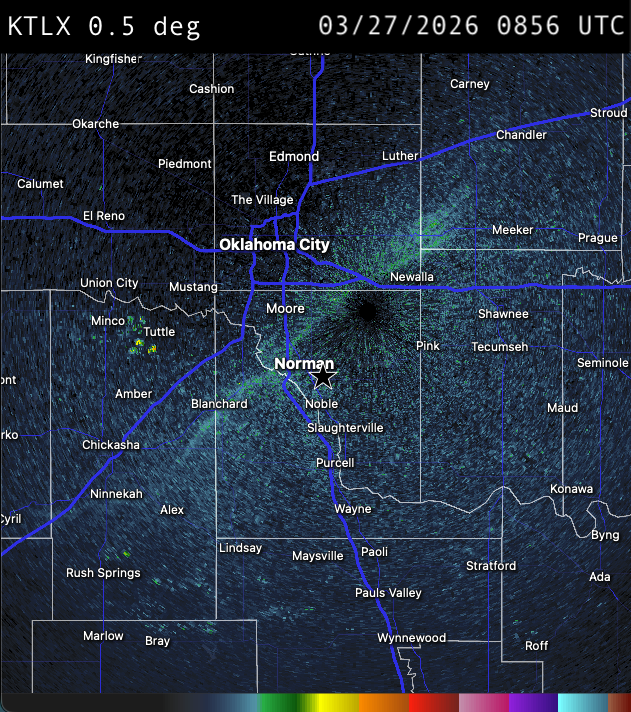
\includegraphics[width=0.92\textwidth]{../../images/fropa_c2_KTLX_88D_20230327_0900.png}
  \caption{KTLX 88D reflectivity at 09:00 UTC.
  KTLX 88D reflectivity fine line and radial velocity discontinuity over Norman at 08:56 UTC, verifying synoptic cold-frontal timing against in situ observations.}
  \label{fig:fropa_c2:fropa_c2_ktlx_88d_20230327_0900}
\end{figure}
\begin{figure}[htbp]
  \centering
  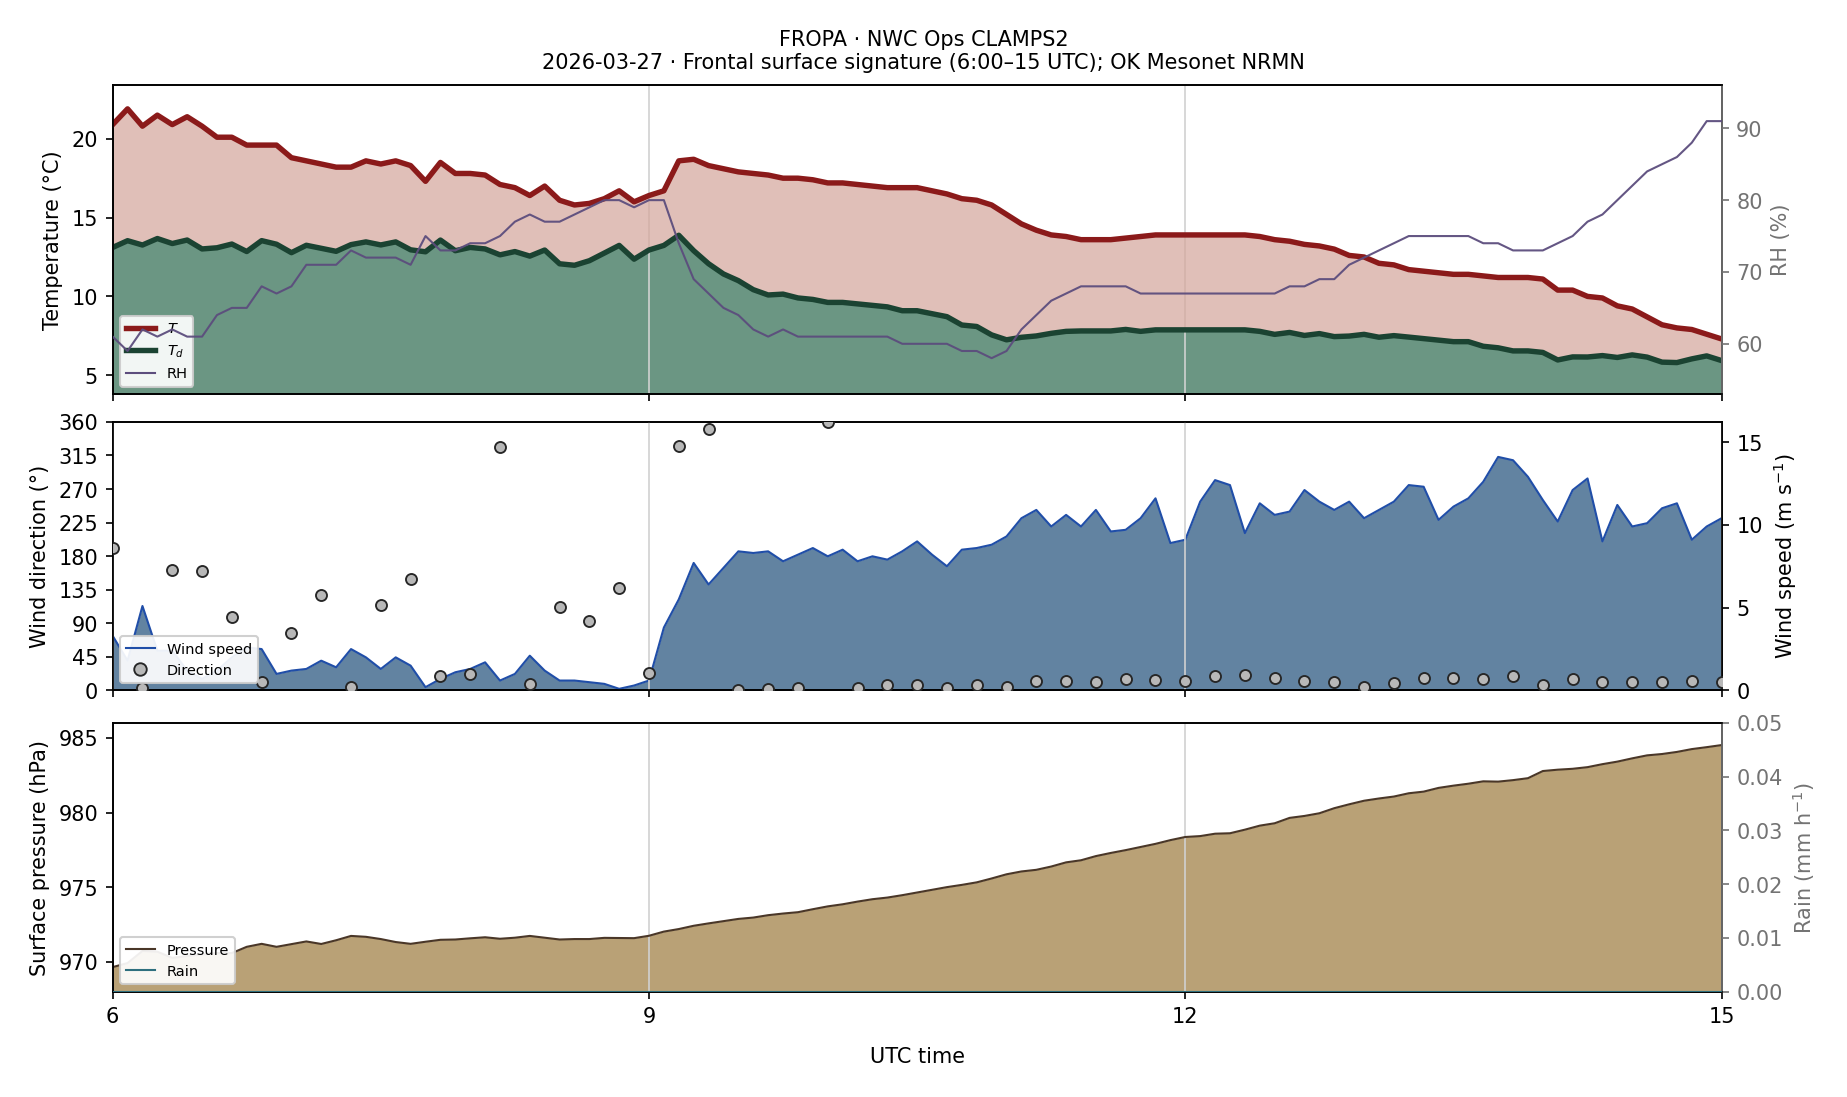
\includegraphics[width=0.92\textwidth]{../../images/fropa_c2_aux_surface_meteogram.png}
  \caption{Norman Mesonet surface meteogram (06–15 UTC).
  Norman Mesonet NRMN surface observations (06–15 UTC) documenting the 09:00 UTC pressure jump, transient surface warming from inversion mixing, and abrupt wind shift at frontal passage.}
  \label{fig:fropa_c2:fropa_c2_aux_surface_meteogram}
\end{figure}
\begin{figure}[htbp]
  \centering
  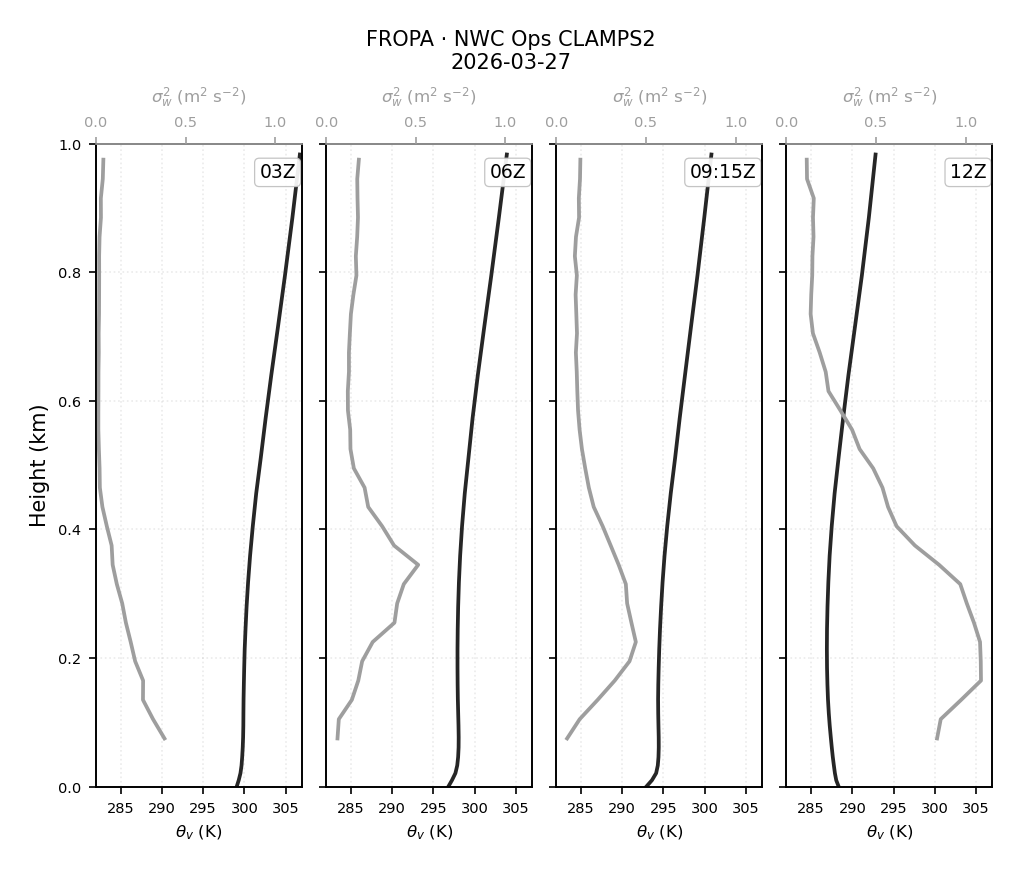
\includegraphics[width=0.92\textwidth]{../../images/fropa_c2_aux_front_theta_sigma_profiles.png}
  \caption{$\theta_v$ and $\sigma_w^2$ profiles at 03, 06, 09:15, and 12 UTC.
  Vertical profiles from the surface to 1 km AGL for $\theta_v$ and from 75 m AGL for $\sigma_w^2$ at four snapshots bracketing frontal passage.}
  \label{fig:fropa_c2:fropa_c2_aux_front_theta_sigma_profiles}
\end{figure}

\end{document}
